\documentclass[11pt]{amsart}
\usepackage{amssymb,amsmath,amsthm}
\usepackage{mathtools}
\usepackage{booktabs}
\usepackage{tikz}
\usetikzlibrary{arrows.meta}
\usepackage[margin=1.15in]{geometry}
\usepackage[colorlinks=true,linkcolor=blue,citecolor=blue,urlcolor=blue]{hyperref}

\numberwithin{equation}{section}
\numberwithin{table}{section}
\numberwithin{figure}{section}

\newtheorem{theorem}{Theorem}[section]
\newtheorem{lemma}[theorem]{Lemma}
\newtheorem{proposition}[theorem]{Proposition}
\newtheorem{corollary}[theorem]{Corollary}
\newtheorem{conjecture}[theorem]{Conjecture}
\theoremstyle{definition}
\newtheorem{definition}[theorem]{Definition}
\theoremstyle{remark}
\newtheorem{remark}[theorem]{Remark}

% Number sets, differentials, operators.
\newcommand{\R}{\mathbb{R}}
\newcommand{\C}{\mathbb{C}}
\newcommand{\N}{\mathbb{N}}
\newcommand{\diff}{\,\mathrm{d}}
\DeclareMathOperator{\supp}{supp}
\DeclareMathOperator{\Log}{Log}
\DeclareMathOperator{\re}{Re}
\DeclareMathOperator{\im}{Im}
\DeclareMathOperator*{\Res}{Res}
\newcommand{\eps}{\varepsilon}
% Cauchy operator and the class of boundary values of Cauchy integrals.
\newcommand{\Cauchy}{\mathcal{C}}
\newcommand{\dC}{\partial\mathcal{C}}
% Angles and regions of the Riemann--Hilbert analysis.
\newcommand{\thlip}{\vartheta_{\mathrm{lip}}}
\newcommand{\thw}{\vartheta_{\mathrm{w}}}
\newcommand{\thseam}{\vartheta_{\mathrm{seam}}}
\newcommand{\Ob}{\Omega_{\mathrm{b}}}
\newcommand{\Osat}{\Omega^{\triangle}}
\newcommand{\Oinf}{\Omega_{\infty}}
\newcommand{\Sin}{S_{\mathrm{in}}}
\newcommand{\Sout}{S_{\mathrm{out}}}
\newcommand{\Sseam}{\Sigma^{\mathrm{s}}}
\newcommand{\Zn}{\mathcal{Z}_n}
\newcommand{\tvphi}{\tilde\varphi}
\newcommand{\wn}{\mathsf w_n}
\newcommand{\Hc}{H^{\circ}_n}

\begin{document}

% sec1_intro.tex: title, abstract, Section 1 (Introduction).
% Labels defined here: sec:intro, sec:results, sec:context, sec:strategy, sec:organisation, eq:sigma, eq:jacobi,
%   eq:cp, eq:law, eq:epsLambda, eq:paper1-averaged, def:analytic, thm:analytic, cor:pure, thm:onen, rem:scope,
%   rem:lommel.

\title[Recurrence coefficients with power-law atoms]{Recurrence coefficients of discrete measures with power-law
atoms: pointwise asymptotics and the $1/n$ term}
\author{Gordon [Surname]}
\date{Draft of 15 October 2026}

\begin{abstract}
Let $\sigma=\sum_{k\ge1}k^{-s}\ell(k)\,\delta_{k^{-p}}$ with $p>0$ and $s>1$, so that its Jacobi matrix is a compact
operator with eigenvalues $k^{-p}$. A previous paper established that the recurrence coefficients satisfy
$n^pb_n\to c(p)$ in a double Ces\`aro sense, with an explicit constant $c(p)$ that comes from a constrained equilibrium
problem. Here we prove the pointwise law $n^pb_n=c(p)(1+O(1/n))$ and $a_n/(2b_n)=1+O(1/n)$ for every $p>0$ and $s>1$,
both for pure powers ($\ell\equiv1$) and for every factor $\ell$ that extends to a slowly varying analytic function in a
sector $|\arg t|\le\vartheta$, however small $\vartheta>0$ is. For pure powers with $p>1$ we also find the $1/n$ term:
$n^pb_n=c(p)(1-(s-1)/(2n)+O(n^{-2}))$ and $n^pa_n=2c(p)(1-(s-1+p)/(2n)+O(n^{-2}))$. The proof is a Riemann--Hilbert
analysis of discrete orthogonal polynomials whose nodes accumulate at a hard edge. The outer scalar function depends on
whether $p$ is larger than, equal to or smaller than $1$. At the hard edge a non-analytic slowly varying factor is
handled by a comparison, in the manner of Conway and Deift, with an explicitly solvable Bessel model; this needs the
Bessel order $(s-1-p)/p$ to lie in $(-1,1)$. A Christoffel transformation, which shifts $s$ by $p$ and preserves the
law together with its rate, removes the restriction.
\end{abstract}

\maketitle

\section{Introduction}\label{sec:intro}

A compact Jacobi operator is determined by its spectral measure. If its eigenvalues are $k^{-p}$ and its spectral
weights decay like $k^{-s}$, how do its matrix entries behave? For $p>0$, $s>1$ and a sequence
$\ell\colon\N\to(0,\infty)$ we study the discrete measure
\begin{equation}\label{eq:sigma}
  \sigma_{p,s,\ell}:=\sum_{k\ge1}k^{-s}\ell(k)\,\delta_{k^{-p}},\qquad \sigma_{p,s}:=\sigma_{p,s,1}.
\end{equation}
It lives on $(0,1]$, and its atoms accumulate only at $0$. Let $P_n$ be its monic orthogonal polynomials and
$h_n:=\int P_n^2\diff\sigma$. They satisfy the three-term recurrence
\begin{equation}\label{eq:jacobi}
  xP_n=P_{n+1}+a_nP_n+b_n^2P_{n-1}\qquad(n\ge0,\ b_0:=0,\ b_n>0),
\end{equation}
so that $b_n^2=h_n/h_{n-1}$; the numbers $a_n$ and $b_n$ are the entries of the Jacobi matrix of $\sigma$. With
\begin{equation}\label{eq:cp}
  I(p):=\frac{\sqrt\pi}{2}\,\frac{\Gamma(\frac1p+\frac12)}{\Gamma(\frac1p+1)},\qquad
  c(p):=\frac14\Bigl(\frac{\pi}{2I(p)}\Bigr)^{p},
\end{equation}
for example $c(1)=\frac12$ and $c(2)=\pi^2/16$, the question is whether
\begin{equation}\label{eq:law}
  n^pb_n\longrightarrow c(p)\qquad\text{and}\qquad n^pa_n\longrightarrow2c(p)\qquad(n\to\infty),
\end{equation}
and at what rate. We call \eqref{eq:law} the \emph{pointwise law}. The constant $c(p)$ comes from the companion paper
\cite{Paper1}, which proves the first half of \eqref{eq:law} in an averaged sense (see \eqref{eq:paper1-averaged}
below).

\subsection{Results}\label{sec:results}
The slowly varying factors we allow are those that extend analytically to a sector, written in the logarithmic
variable $\xi=\log t$.

\begin{definition}[analytic slowly varying factors]\label{def:analytic}
Let $\vartheta>0$. A sequence $\ell\colon\N\to(0,\infty)$ is \emph{analytic of angle $\vartheta$} if
$\ell(k)=\exp\Lambda(\log k)$ for all $k\ge1$, where, for some $c_0>0$, the function $\Lambda$ is analytic on
$S_\vartheta:=\{\xi\in\C:\ \re\xi\ge-c_0,\ |\im\xi|\le\vartheta\}$, real on $S_\vartheta\cap\R$, bounded on
$S_\vartheta\cap\{\re\xi\le0\}$, and
\begin{equation}\label{eq:epsLambda}
  \varepsilon_\Lambda(T):=\sup\bigl\{|\Lambda'(\xi)|:\ \xi\in S_\vartheta,\ \re\xi\ge T\bigr\}\longrightarrow0
  \qquad(T\to\infty).
\end{equation}
We then also say that $\Lambda$ is analytic of angle $\vartheta$. If $\vartheta'<\vartheta$, a sequence that is
analytic of angle $\vartheta$ is also analytic of angle $\vartheta'$.
\end{definition}

Such an $\ell$ is slowly varying. The angle may be arbitrarily small, because the Riemann--Hilbert analysis evaluates
the weight only in a sector whose opening we are free to shrink (Lemma~\ref{lem:weightdomain} and
Remark~\ref{rem:angles}). For example, $\exp\sqrt{\log(k+e)}$ and $(\log(k+e))^\beta$, $\beta\in\R$, are analytic of
every angle $\vartheta<\pi$, while $\Lambda(\xi)=\sqrt{\xi+1}+(\xi+2)^{-1/2}\log(1-q\cos2\xi)$ with $q=1/\cosh(0.6)$
has logarithmic branch points at $\xi=\pi m\pm0.3i$, $m\in\mathbb Z$, and is analytic only of the angles
$\vartheta<0.3$ (Section~\ref{sec:numerics}).

\begin{theorem}\label{thm:analytic}
Let $p>0$ and $s>1$, and let $\ell$ be analytic of angle $\vartheta$ for some $\vartheta>0$. Then the Jacobi
coefficients of $\sigma_{p,s,\ell}$ satisfy, as $n\to\infty$,
\[
  n^pb_n=c(p)\bigl(1+O(1/n)\bigr),\qquad \frac{a_n}{2b_n}=1+O(1/n),
\]
with constants depending on $p$, $s$ and $\ell$.
\end{theorem}

The constant sequence $\ell\equiv1$ is analytic of every angle, with $\Lambda\equiv0$.

\begin{corollary}[pure powers]\label{cor:pure}
For every $p>0$ and $s>1$ the measure $\sigma_{p,s}$ satisfies $n^pb_n=c(p)(1+O(1/n))$ and $a_n/(2b_n)=1+O(1/n)$.
In particular, for real $a>0$ and $b$ with $2a+b>1$, the measure $\sigma_{a,2a+b}$ has the moments
$\zeta(aj+2a+b)$, $j\ge0$, and Hankel determinants $\det_{1\le i,j\le n}\zeta(a(i+j)+b)$
\textup{(}\cite[Corollary~1.4 and its proof]{Paper1}\textup{)}, and its recurrence coefficients satisfy
$n^ab_n=c(a)(1+O(1/n))$ and $a_n/(2b_n)=1+O(1/n)$.
\end{corollary}

For pure powers with $p>1$ we identify the next term.

\begin{theorem}\label{thm:onen}
Let $p>1$ and $s>1$. Then the Jacobi coefficients of $\sigma_{p,s}$ satisfy, as $n\to\infty$,
\[
  n^pb_n=c(p)\Bigl(1-\frac{s-1}{2n}+O(n^{-2})\Bigr),\qquad
  n^pa_n=2c(p)\Bigl(1-\frac{s-1+p}{2n}+O(n^{-2})\Bigr).
\]
Consequently $a_n/(2b_n)=1-p/(2n)+O(n^{-2})$ and $b_n=c(p)\bigl(n+\frac{s-1}{2p}\bigr)^{-p}\bigl(1+O(n^{-2})\bigr)$.
\end{theorem}

Here, as everywhere in this paper, $a_n/(2b_n)$ pairs the diagonal entry at $P_n$ with the off-diagonal entry $b_n$
between $P_{n-1}$ and $P_n$, as in \eqref{eq:jacobi}.

The proofs use the following external results, each stated with its hypotheses in
\S\S\ref{sec:tool-wlxz}--\ref{sec:tool-dlmf}. For Theorem~\ref{thm:analytic}: the formulation of the discrete
Riemann--Hilbert problem by Wu, Lin, Xu and Zhao \cite{WLXZ}, as a pattern only (none of their theorems is applied);
the explicit Bessel model of Kuijlaars, McLaughlin, Van Assche and Vanlessen \cite[\S6]{KMVV}, including its freedom
in the choice of angle; Theorem~4.4 of Conway and Deift \cite{CD}, together with the argument of their Theorem~4.7
and Proposition~4.9 and one direction of their Proposition~4.6, which we re-prove; and special-function facts from
\cite{DLMF}. Theorem~\ref{thm:onen} uses in addition the classical left-endpoint Bessel parametrix of
\cite[(6.42)--(6.53)]{KMVV} and the expansions \cite[\S\S9.7, 10.17, 10.40]{DLMF}. The Laurent coefficients of the
first corrections that enter the proof of Theorem~\ref{thm:onen} (Section~\ref{sec:second} and
Appendix~\ref{app:residues}) were computed by exact symbolic series expansion; the coefficient at the hard edge was
also computed by hand.

\begin{remark}[what is, and is not, proved at order $1/n$]\label{rem:scope}
Theorem~\ref{thm:analytic} bounds the deviation from $c(p)$ at order $1/n$ but does not identify the $1/n$ term. The
proof compares the true problem with an exactly solvable comparison problem: relative to it, the non-analytic part of
$\ell$ moves the first two coefficients at infinity by $o(1/n)$ (Section~\ref{sec:hardedge}), but the comparison
problem itself depends on $\ell$ at order $1/n$. So the $O(1/n)$ is absolute, not relative: we do not claim that
$b_n(\sigma_{p,s,\ell})/b_n(\sigma_{p,s})-1=O(\varepsilon_\Lambda(\log n)/n)$. Conjectures for the $1/n$ term when
$p\le1$ or $\ell\not\equiv1$ are formulated in Section~\ref{sec:further} (Conjectures~\ref{conj:onen}
and~\ref{conj:tilt}).
\end{remark}

\begin{remark}[a classical instance]\label{rem:lommel}
For $(p,s)=(2,2)$ the coefficients are explicit. Van Assche \cite[\S3]{VA} records that the orthonormal Lommel
polynomials satisfy $xp_n=\beta_{n+1}p_{n+1}+\beta_np_{n-1}$ with $\beta_{n+1}=[2\sqrt{(n+\nu)(n+\nu+1)}]^{-1}$. For
$\nu=\frac32$ the orthogonality measure $\mu$ is identified as follows. By the Bessel recurrence
\cite[(10.6.1)]{DLMF}, $\mathsf u_n:=\sqrt{n+\nu}\,J_{\nu+n}(1/x)$ solves $x\mathsf u_n=\beta_{n+1}\mathsf
u_{n+1}+\beta_n\mathsf u_{n-1}$ for $n\ge0$ (with $\beta_0:=[2\sqrt{\nu(\nu-1)}]^{-1}$), and it is square summable by
\cite[(10.2.2)]{DLMF}. For $x\notin\R$ the resolvent vector $(\mathcal J-x)^{-1}e_0$ of the Jacobi matrix $\mathcal J$
solves the same recurrence for $n\ge1$ and is square summable, and such solutions form a line, since the Wronskian
$\beta_n(\mathsf u_n\tilde{\mathsf u}_{n-1}-\mathsf u_{n-1}\tilde{\mathsf u}_n)$ of two of them is constant and tends to $0$. Hence
$\int(t-x)^{-1}\diff\mu(t)$, the first entry of the resolvent, equals $-\mathsf u_0/(\beta_0\mathsf u_{-1})=-2\nu
J_\nu(1/x)/J_{\nu-1}(1/x)$. For $\nu=\frac32$ this is $-3(z^{-1}-\cot z)$ with $z=1/x$ \cite[(10.16.1),
(10.6.1)]{DLMF}, and the partial fractions of $\cot$ \cite[(4.22.3)]{DLMF} show that $\mu$ has mass $3/(\pi k)^2$ at
$\pm1/(\pi k)$, $k\ge1$. Its image under $t\mapsto\pi^2t^2$ is $(6/\pi^2)\sigma_{2,2}$. The quadratic transformation
(the monic orthogonal polynomials of $\mu$ of degree $2n$ are $q_n(t^2)$, where $q_n$ are those of the image of $\mu$
under $t\mapsto t^2$) gives $a_n=\pi^2(\beta_{2n}^2+\beta_{2n+1}^2)$ and $b_n=\pi^2\beta_{2n-1}\beta_{2n}$ for
$\sigma_{2,2}$, that is,
\[
  b_n=\frac{\pi^2}{(4n+1)\sqrt{(4n-1)(4n+3)}},\qquad a_n=\frac{2\pi^2}{(4n+1)(4n+5)}\qquad(n\ge1).
\]
Thus $n^2b_n/c(2)=1-\frac1{2n}+O(n^{-2})$ and $a_n/(2b_n)=1-\frac1n+O(n^{-2})$, in agreement with
Theorem~\ref{thm:onen} at $(p,s)=(2,2)$.
\end{remark}

\subsection{Context}\label{sec:context}
\emph{Why the pointwise law is subtle.} By \cite[Corollary~1.2]{Paper1}, specialised to the atoms $x_k=k^{-p}$, if
the weights $w_k\ge0$ satisfy $\sum_kw_k<\infty$ and $w_k\ge c_1k^{-s'}$ for some constants $c_1>0$ and $s'\in\R$,
then the recurrence coefficients of $\sum_kw_k\delta_{k^{-p}}$ satisfy
\begin{equation}\label{eq:paper1-averaged}
  \frac{2}{n^2}\sum_{j=1}^{n-1}(n-j)\log\bigl(j^pb_j\bigr)\longrightarrow\log c(p).
\end{equation}
The constant comes from an explicitly solvable constrained equilibrium problem \cite[Theorem~1.3]{Paper1}, whose
solution $\mu^*$ is the zero distribution that a Jacobi matrix with entries $a_n\approx2b_n\approx2c(p)n^{-p}$ would
produce. But \eqref{eq:paper1-averaged} is a double Ces\`aro mean of $\log(j^pb_j)$, that is, a statement about the
logarithm of the Hankel determinant $D_n$ of $\sigma$ at order $n^2$. Multiplying the weights by factors in
$[e^{-\varepsilon},e^{\varepsilon}]$ changes $\log D_n$ by at most $\varepsilon n$, so the averaged law cannot see such
perturbations, and passing from it to \eqref{eq:law} is a Tauberian step that needs a regularity of $j^pb_j$ which the
averaged argument does not provide; it has to come from the weights. The companion paper \cite{Paper3}
uses the results of this paper to treat general slowly varying and rough weights, and shows there that bounded rough
weights can break the pointwise law.

\emph{Discrete orthogonal polynomials.} The Riemann--Hilbert approach to discrete orthogonal polynomials was developed
by Baik, Kriecherbauer, McLaughlin and Miller \cite{BKMM} for measures on finite node sets in a bounded interval, with
real-analytic node density and potential; their analysis includes saturated regions, which also appear here. Within
the literature we have read, the only Riemann--Hilbert analysis of discrete orthogonal polynomials on infinitely many
nodes accumulating at a finite point is that of Wu, Lin, Xu and Zhao \cite{WLXZ}, for the Tricomi--Carlitz
polynomials; our frame follows theirs. Dai and Yao make the same observation: ``Wu et al.\ [21] studied the case where
the orthogonality lattice consists of infinite nodes with an accumulation point. Except [21], the orthogonality
lattices are always equally spaced'' \cite[\S1]{DY}, [21] being \cite{WLXZ}.

\emph{Non-analytic weights.} Our weights are not analytic at the hard edge, and the standard local parametrix does not
exist there. Conway and Deift \cite{CD} met the same difficulty for the weight $\log\frac{2k}{1-x}$ on $(-1,1)$, which
carries a slowly varying factor at the endpoint $x=1$; they write that ``there is no known parametrix for the
Riemann--Hilbert problem in a neighborhood of the logarithmic singularity at $x=1$'', and they compare the problem with
the Legendre problem through the operator theory behind Riemann--Hilbert problems instead of through a quotient. The
comparison argument of Section~\ref{sec:hardedge} is theirs \cite[Theorem~4.7 and Proposition~4.9]{CD}. What we add
is a comparison model built from the Szeg\H{o} function of the full weight (an explicit parametrix rather than a second
orthogonality problem), a uniform resolvent bound for a Bessel edge of any order $|\alpha|<1$ (rather than the Legendre
value $\alpha=0$), and the treatment of an arbitrary analytic slowly varying factor (rather than one explicit
logarithm). Deift and Piorkowski \cite{DP} extended the
analysis of \cite{CD} to the weight $\log\frac{2}{1-x}$ and write, about a comparison with a weight that has a simple
zero at the endpoint: ``the crucial Theorem~4.7 in [4] requires a different proof in this case: now one needs to
control the behaviour of the Cauchy operator acting on spaces with Muckenhoupt weights'' \cite[\S1]{DP}, [4] being
\cite{CD}. This is consistent with our restriction to Bessel orders $|\alpha|<1$ in the comparison step
(Remark~\ref{rem:alpha-ge-1}). Other approaches to non-analytic weights are Piorkowski's parametrix-free method, which
needs an a priori estimate for the exact solution \cite{Pio}; the $\bar\partial$ methods of McLaughlin and Miller
\cite{MM} and of Trogdon \cite{Tro}, which assume a finite number of Lipschitz derivatives of the weight (for
\cite{Tro}, $C^{k,1}$ regularity up to the endpoints of the support); and the approximation of a smooth symbol by
analytic ones in Deift, Its and Krasovsky \cite[\S6.2]{DIK}.

\emph{Recurrence asymptotics without analyticity.} For exponential weights $W=e^{-Q}$, Levin and Lubinsky \cite{LL}
prove $o(1)$ asymptotics of the recurrence coefficients, with constants given by equilibrium quantities, under
regularity conditions that do not involve analyticity, and without Riemann--Hilbert methods.

\emph{Special cases.} Besides the Lommel case (Remark~\ref{rem:lommel}), we mention the Hankel determinants of zeta
values studied by Monien \cite{Monien} and by Haynes and Zudilin \cite{HaynesZudilin}; for $a=1$ Monien reports a full
asymptotic expansion of the determinants, obtained numerically by D.~Zagier, which goes beyond
Corollary~\ref{cor:pure} but is not proved. The Tricomi--Carlitz polynomials are orthogonal with respect to a measure on the points $\pm1/\sqrt{k+t_0}$, for a
parameter $t_0>0$ \cite[\S3]{VA}; in the squared variable this is an instance of $p=1$ with weights that are not pure
powers. Their recurrence coefficients are explicit \cite[\S3]{VA}, and \cite{WLXZ} obtain uniform asymptotics of the
polynomials.

\subsection{Method}\label{sec:strategy}
The proof of Theorem~\ref{thm:analytic} has an elementary part and a Riemann--Hilbert part. The elementary part is the
Christoffel shift, Theorem~\ref{thm:shift}: the pointwise law passes from $\sigma$ to $x\sigma$ together with any
regular rate, and $x\sigma_{p,s,\ell}=\sigma_{p,s+p,\ell}$. What is new there is the rate; the statement without rate
follows from a proposition of Dai, Piao and Qiao \cite[Proposition~2.1]{DPQ} and the classical transfer formulas
\cite[\S1]{DD}. The shift reduces Theorem~\ref{thm:analytic} to the window $1<s<1+2p$, where the Bessel order
$\alpha:=(s-1-p)/p$ of the hard edge lies in $(-1,1)$ (Theorem~\ref{thm:window}). For the Riemann--Hilbert part we
rescale $z\mapsto n^pz$. The equilibrium measure $\mu^*$ of \cite{Paper1} then has the band $(0,4c(p))$, where the
polynomials oscillate, the saturated region $(4c(p),\infty)$, where their zeros follow the nodes, and a soft edge at
$4c(p)$, and on it we build one frame for all $p>0$ (Section~\ref{sec:frame}). The three geometries $p>1$, $p=1$ and
$p<1$ enter only through the outer scalar function that removes the Gamma-function growth of the node masses
(Section~\ref{sec:outer} and Appendix~\ref{app:outer}): the index function $t(z)=nz^{-1/p}$ maps the slit plane onto a
sector that lies inside, exactly fills, or exceeds the sector where Stirling's formula holds. At the hard edge the
factor enters through $r_n(z)=\ell(nz^{-1/p})/\ell(n)$, which is not analytic at $0$, so the classical Bessel
parametrix is not available. Following Conway and Deift, we compare the problem with a Bessel model built from the
Szeg\H{o} function of the whole band weight; the two problems differ on the lips of the lens by $o(1)$ without a rate,
and for $|\alpha|<1$ a uniform resolvent bound and Bessel localisation turn this into an $O(1/n)$ error in the
coefficients (Section~\ref{sec:hardedge}). For $\ell\equiv1$ and $p>1$ the classical Bessel parametrix does apply, for
every $\alpha>-1$ (Section~\ref{sec:classical}), and it gives the $1/n$ term (Section~\ref{sec:second}): the band factor
is constant up to $O(n^{-p})$, the hard-edge correction is annihilated by both functionals that extract $a_n$ and $b_n$,
and the $1/n$ term comes from the Airy correction at the soft edge. This module cannot handle a non-analytic $r_n$, it
fails at $p=1$, and we do not use it for $p<1$, where the band factor is not constant to $o(1/n)$ near $0$.

\subsection{Organisation}\label{sec:organisation}
Section~\ref{sec:prelim} fixes conventions and states the inputs, and Section~\ref{sec:shift} proves
Theorem~\ref{thm:shift}. Sections~\ref{sec:frame}--\ref{sec:extraction} prove Theorem~\ref{thm:window} and, with the
shift, Theorem~\ref{thm:analytic} and Corollary~\ref{cor:pure}; the interface between the frame and the hard edge is
Proposition~\ref{prop:frame}. Sections~\ref{sec:classical} and~\ref{sec:second} prove Theorem~\ref{thm:onen},
Section~\ref{sec:numerics} gives numerical illustrations, and Section~\ref{sec:further} contains conjectures and open
problems. A reader interested only in Theorem~\ref{thm:onen} needs Sections~\ref{sec:prelim}, \ref{sec:frame},
\ref{sec:outer}, \ref{sec:classical} and~\ref{sec:second} and Appendices~\ref{app:outer} and~\ref{app:residues}, and
nothing from Section~\ref{sec:hardedge}.

Throughout, $n$ is the degree, and $C,C'$ denote positive constants that may change from line to line. They are
never written $c$, which is reserved for $c(p)$; the exceptions are $c_0$ in Definition~\ref{def:analytic} and $c_1$ in
\eqref{eq:paper1-averaged}. Our atoms are exactly $k^{-p}$, so the atom constant of \cite[Theorem~1.1]{Paper1} does not
appear.

% sec2_prelim.tex: Section 2 (Preliminaries).
% Labels defined here: sec:prelim, sec:prelim-op, sec:prelim-rates, sec:prelim-eq, sec:tool-wlxz, sec:tool-bessel,
%   sec:tool-cd, sec:tool-dlmf, eq:rec-monic, eq:rec-orth, eq:coef-int, def:regular, eq:regular-facts,
%   rem:majorant, prop:equilibrium, eq:Y-solution, eq:Y-extract, eq:CD-moments.

\section{Preliminaries}\label{sec:prelim}

This section fixes conventions and collects the inputs of the proofs. The only input from the companion
paper~\cite{Paper1} is the explicit equilibrium measure (\S\ref{sec:prelim-eq}). Every external result used later is
stated in \S\S\ref{sec:tool-wlxz}--\ref{sec:tool-dlmf}, with its hypotheses and the equation numbers of the source,
so that the later sections can refer to it by subsection and part.

\emph{Notation used throughout.} The data are $p>0$, $s>1$ and $\ell$; the function $\Lambda$, the modulus
$\varepsilon_\Lambda$ and the notion ``analytic of angle $\vartheta$'' are those of Definition~\ref{def:analytic}, and
$c=c(p)$ is given by \eqref{eq:cp}. The Bessel order of the hard edge is $\alpha:=(s-1-p)/p$, so that $\alpha>-1$ for
every $s>1$. Sections~\ref{sec:frame} and~\ref{sec:outer} hold for every $\alpha>-1$ and every $\ell$ that is analytic
of some angle; Sections~\ref{sec:hardedge} and~\ref{sec:extraction} assume $|\alpha|<1$, that is, $1<s<1+2p$; and
Sections~\ref{sec:classical} and~\ref{sec:second} assume $p>1$ and $\ell\equiv1$. The Riemann--Hilbert notation is
introduced in Section~\ref{sec:frame}, and Table~\ref{tab:geometry} lists the quantities that depend on whether $p>1$,
$p=1$ or $p<1$. Symbols used only inside one proof are local to it. We write $\mathbb D(z_0,r)$ for the open disc of
radius $r$ about $z_0$, and $\C_\pm$ for the open upper and lower half-planes.

\subsection{Orthogonal polynomials and recurrence coefficients}\label{sec:prelim-op}

Let $\sigma$ be a positive Borel measure on $[0,\infty)$ with infinite support and finite moments. Its Hankel
determinants are positive, so the monic orthogonal polynomials $P_n$ ($\deg P_n=n$) exist for every $n\ge0$. Put
$h_n:=\int P_n^2\diff\sigma>0$, $P_{-1}:=0$ and $b_0:=0$. The polynomials satisfy the three-term recurrence
\begin{equation}\label{eq:rec-monic}
  xP_n=P_{n+1}+a_nP_n+b_n^2P_{n-1}\qquad(n\ge0),\qquad b_n^2=\frac{h_n}{h_{n-1}}\quad(n\ge1),
\end{equation}
with $a_n\in\R$ and $b_n>0$ for $n\ge1$. We call $a_n$ and $b_n$ the \emph{recurrence coefficients} of
$\sigma$. Multiplying $\sigma$ by a positive constant does not change them. The orthonormal polynomials $p_n:=P_n/\sqrt{h_n}$
satisfy
\begin{equation}\label{eq:rec-orth}
  xp_n=b_{n+1}p_{n+1}+a_np_n+b_np_{n-1}\qquad(n\ge0),
\end{equation}
as one sees by dividing \eqref{eq:rec-monic} by $\sqrt{h_n}$ and using $b_n^2\sqrt{h_{n-1}/h_n}=b_n$. Since $xp_j$ has
degree $j+1$, orthonormality gives
\begin{equation}\label{eq:coef-int}
  a_n=\int xp_n^2\diff\sigma,\qquad b_n=\int xp_{n-1}p_n\diff\sigma,\qquad \int xp_np_j\diff\sigma=0\quad(j\le n-2).
\end{equation}
In matrix form, \eqref{eq:rec-orth} says that the Jacobi matrix of $\sigma$ is the symmetric tridiagonal matrix
$\mathcal J(\sigma)$ with diagonal $(a_0,a_1,\dots)$ and off-diagonal $(b_1,b_2,\dots)$. The monic form
\eqref{eq:rec-monic} corresponds to the non-symmetric matrix $J=J(\sigma)$ with $J_{n,n}=a_n$, $J_{n,n+1}=1$ and
$J_{n+1,n}=b_{n+1}^2$; this is the form used in Section~\ref{sec:shift}. The ratio $a_n/(2b_n)$ always pairs the
diagonal entry at $P_n$ with the off-diagonal entry $b_n$ between $P_{n-1}$ and $P_n$; both are read off from the same
Riemann--Hilbert matrix of degree $n$ (Proposition~\ref{prop:frame}(viii)).

If $\ell$ is analytic of angle $\vartheta$ for some $\vartheta>0$, then $\ell(k)\le C_\eta k^\eta$ for every $\eta>0$
by the Potter bound of Lemma~\ref{lem:pottersector}(i). Taking $\eta<s-1$ shows that $\sigma_{p,s,\ell}$ is a finite
measure on $(0,1]$ with infinitely many atoms, so everything above applies to it.

\subsection{Regular rates}\label{sec:prelim-rates}

\begin{definition}\label{def:regular}
A sequence $(\eta_n)_{n\ge1}$ of positive numbers is a \emph{regular rate} if $\eta_n$ is non-increasing, $n\eta_n$ is
non-decreasing, and $\eta_n\to0$.
\end{definition}

The basic example is $\eta_n=1/n$. Every regular rate satisfies
\begin{equation}\label{eq:regular-facts}
  \frac1n\le\frac{\eta_n}{\eta_1},\qquad \eta_{n-1}\le2\eta_n\quad(n\ge2),\qquad \sum_n\eta_n=\infty .
\end{equation}
The first holds because $n\eta_n\ge\eta_1$; the second because $(n-1)\eta_{n-1}\le n\eta_n$; the third follows from
the first.

\begin{remark}[Regular majorants]\label{rem:majorant}
Every non-increasing sequence $\mathsf v_n>0$ with $\mathsf v_n\to0$ is dominated by a regular rate, namely
$\eta_n:=\max_{m\le n}(m\mathsf v_m)/n$. Here $\eta_n\ge\mathsf v_n$ and $n\eta_n$ is non-decreasing by construction;
$\eta_{n+1}\le\max\bigl(\eta_n\,n/(n+1),\mathsf v_{n+1}\bigr)\le\eta_n$ because $\mathsf v_{n+1}\le\mathsf v_n\le\eta_n$;
and $\eta_n\to0$, since $m\mathsf v_m/n\le\mathsf v_1/\sqrt n$ for $m\le\sqrt n$ and $m\mathsf v_m/n\le\mathsf
v_{\lceil\sqrt n\rceil}$ for $\sqrt n<m\le n$. So Theorem~\ref{thm:shift} applies to any monotone rate. In this paper we
use it only with $\eta_n=1/n$.
\end{remark}

\subsection{The equilibrium measure}\label{sec:prelim-eq}

The Riemann--Hilbert analysis of Sections~\ref{sec:frame}--\ref{sec:second} is built on the equilibrium measure of the
constrained problem solved in~\cite{Paper1}. We use only its explicit form and the equality of its potential on the
band; the optimality statement \cite[Theorem~1.3(iii)]{Paper1} is not used in this paper.

Let $c=c(p)$, let $\gamma_p:=\log c(p)+p$, and let $\lambda_p(x):=\frac1px^{-1-1/p}$ be the density of the nodes
$k^{-p}$ (the image of Lebesgue measure on $(0,\infty)$ under $u\mapsto u^{-p}$). For $y\in[0,1]$ and $a',b'>0$ write
$\mathcal B_y(a',b'):=B(a',b')^{-1}\int_0^yr^{a'-1}(1-r)^{b'-1}\diff r$ for the regularised incomplete beta function,
where $B$ is Euler's Beta function. For $\beta>0$ let $\mathrm{arc}_\beta$ be the arcsine law on $[0,\beta]$, with
density $1/(\pi\sqrt{y(\beta-y)})$, and put $\beta_\tau:=4c\tau^{-p}$ for $0<\tau\le1$.

\begin{proposition}\label{prop:equilibrium}
Let $p>0$ and let $\mu^*:=\int_0^1\mathrm{arc}_{\beta_\tau}\diff\tau$, a probability measure on $(0,\infty)$.
\begin{enumerate}
\item[\textup{(i)}] $\mu^*$ has the density
  \[
    \psi^*(x)=\lambda_p(x)\,\mathcal B_{\min(1,\,x/4c)}\bigl(\tfrac1p+\tfrac12,\tfrac12\bigr),\qquad x>0 .
  \]
  In particular $\psi^*=\lambda_p$ on $[4c,\infty)$ (saturation) and $0<\psi^*<\lambda_p$ on $(0,4c)$.
\item[\textup{(ii)}] The function $U^*(x):=\int\log|x-y|\diff\mu^*(y)$ satisfies $U^*(x)=\gamma_p$ for $0<x\le4c$, and
  $U^*(x)\ge\gamma_p$ for all $x>0$.
\item[\textup{(iii)}] \textup{(}Hard edge.\textup{)} As $x\to0^+$,
  \[
    \psi^*(x)=C_*x^{-1/2}\bigl(1+O(x)\bigr),\qquad C_*:=\frac{(4c)^{-1/p-1/2}}{p\,a_*B(a_*,\frac12)},\quad
    a_*:=\frac1p+\frac12 .
  \]
\end{enumerate}
\end{proposition}

\begin{proof}
Parts (i) and (ii) are \cite[Theorem~1.3(i)--(ii)]{Paper1}, transported from the variable $u$ to $x=u^{-p}$. There,
$\mu^*_u$ is the image of $\mu^*$ under $x\mapsto x^{-1/p}$ and has density
$\rho^*(u)=\mathcal B_{\min(1,u^{-p}/4c)}(\frac1p+\frac12,\frac12)$, with $\rho^*=1$ exactly on $(0,(4c)^{-1/p}]$ and
$0<\rho^*<1$ on $((4c)^{-1/p},\infty)$. Since $|\diff u/\diff x|=\lambda_p(x)$, the density of $\mu^*$ in $x$ is
$\lambda_p(x)\rho^*(x^{-1/p})$, which is (i). Part (ii) is quoted verbatim, with $\gamma_p=\log c+p$. For (iii), let
$y=x/4c\le1$. Then $\int_0^yr^{a_*-1}(1-r)^{-1/2}\diff r=\frac{y^{a_*}}{a_*}(1+O(y))$, so
$\psi^*(x)=\frac1px^{-1-1/p}(x/4c)^{1/p+1/2}\bigl(a_*B(a_*,\frac12)\bigr)^{-1}(1+O(x))$, which is (iii).
\end{proof}

The point $x=4c$ is the soft edge, $(0,4c)$ is the band, and $x=0$ is the hard edge, where $\mu^*$ has the
inverse-square-root density of (iii).

\subsection{The discrete interpolation problem of Wu, Lin, Xu and Zhao}\label{sec:tool-wlxz}

This subsection and the next three state the external results used in Sections~\ref{sec:frame}--\ref{sec:second} and
the appendices. They are needed only from Section~\ref{sec:frame} on. Throughout, the Cauchy transform on an oriented
contour $\Sigma$ is
\[
  \Cauchy f(z):=\frac1{2\pi i}\int_\Sigma\frac{f(s)\diff s}{s-z},\qquad z\in\C\setminus\Sigma,
\]
and $\Cauchy_\pm f$ are its non-tangential boundary values from the left ($+$) and the right ($-$) of $\Sigma$, so that
$\Cauchy_+-\Cauchy_-=1$. For a jump matrix $v$ on $\Sigma$ we write $\Cauchy_vf:=\Cauchy_-\bigl(f(v-I)\bigr)$. The
matrices $\sigma_1,\sigma_2,\sigma_3$ are the Pauli matrices, and $\sigma_3=\mathrm{diag}(1,-1)$.

Wu, Lin, Xu and Zhao~\cite{WLXZ} develop the Riemann--Hilbert method for discrete orthogonal polynomials on infinitely
many nodes with an accumulation point, for the Tricomi--Carlitz polynomials. We apply none of their theorems to our
measures; we use the formulation of the problem and the order of the transformations, and our versions are written out
in Sections~\ref{sec:frame} and~\ref{sec:outer}.

\emph{(a) The problem and its solution.} Let $\sigma=\sum_{k\ge1}w_k\delta_{x_k}$ with distinct nodes
$x_k\in(0,1]$, $w_k>0$ and $\sum_kw_k<\infty$, and fix $n\ge1$. Following \cite[(2.14) and Theorem~2.3]{WLXZ}, put
\begin{equation}\label{eq:Y-solution}
  Y(z):=\begin{pmatrix}P_n(z) & \displaystyle\sum_k\frac{w_kP_n(x_k)}{z-x_k}\\[3mm]
  h_{n-1}^{-1}P_{n-1}(z) & \displaystyle h_{n-1}^{-1}\sum_k\frac{w_kP_{n-1}(x_k)}{z-x_k}\end{pmatrix}.
\end{equation}
Then $Y$ is analytic in $\C\setminus(\{x_k\}_k\cup\{0\})$; at each node it has a simple pole with
$\Res_{z=x_k}Y(z)=\lim_{z\to x_k}Y(z)\bigl(\begin{smallmatrix}0&w_k\\0&0\end{smallmatrix}\bigr)$ (the residue
condition \cite[(2.14)]{WLXZ}); and $Y(z)z^{-n\sigma_3}=I+Y_1/z+Y_2/z^2+O(z^{-3})$ as $z\to\infty$, with
\begin{equation}\label{eq:Y-extract}
  (Y_1)_{12}(Y_1)_{21}=b_n^2,\qquad \frac{(Y_2)_{12}}{(Y_1)_{12}}-(Y_1)_{22}=a_n .
\end{equation}
\emph{Proof.} The sums converge locally uniformly off $\{x_k\}\cup\{0\}$, which gives analyticity, the simple poles and
$\Res_{x_k}Y_{j2}=w_kY_{j1}(x_k)$. Write $P_m(x)=x^m+\pi_mx^{m-1}+\dots$. For $|z|>2$, expanding $(z-x)^{-1}$ gives
$\sum_kw_kP_m(x_k)/(z-x_k)=\sum_{i\ge0}z^{-i-1}\int P_mx^i\diff\sigma$, and $\int P_mx^i\diff\sigma$ equals $0$ for $i<m$,
$h_m$ for $i=m$ and $-\pi_{m+1}h_m$ for $i=m+1$. Hence $(Y_1)_{12}=h_n$, $(Y_1)_{21}=h_{n-1}^{-1}$,
$(Y_2)_{12}=-\pi_{n+1}h_n$ and $(Y_1)_{22}=-\pi_n$; and $\pi_n=\pi_{n+1}+a_n$ by \eqref{eq:rec-monic}. \qed

\emph{(b) Transformations.} The transformations of Section~\ref{sec:frame} follow \cite[\S\S3--5]{WLXZ}: removal of the
poles by triangular factors built from $\Pi=\sin\theta/\theta'$ and $e^{\pm i\theta}$ \cite[(3.9)--(3.15)]{WLXZ},
normalisation by the $g$-function \cite[(4.1)]{WLXZ}, the lens and saturated-region factors $V_\pm$, $V^\triangle_\pm$
\cite[(4.12)--(4.13)]{WLXZ}, and conjugation by an outer scalar \cite[(5.1)]{WLXZ}. In \cite{WLXZ} these are written in
a symmetric variable with nodes $\pm x_k$; we use only the pattern, and every jump is recomputed in
Section~\ref{sec:frame} for our one-sided problem.

\emph{(c) The soft edge.} Our Airy parametrix (Lemma~\ref{lem:airy}) follows the pattern of \cite[\S6.1, (6.4),
(6.10)--(6.12)]{WLXZ}; it is constructed from the Airy function directly (\S\ref{sec:tool-dlmf}), and no statement of
\cite{WLXZ} is used.

\subsection{The Bessel model of Kuijlaars, McLaughlin, Van Assche and Vanlessen}\label{sec:tool-bessel}

We use the explicit Bessel model of \cite[\S6]{KMVV} and its algebraic properties. In Sections~\ref{sec:hardedge}
and~\ref{sec:extraction} we apply none of their theorems on orthogonal polynomials, so their standing hypothesis on the
weight \cite[(1.1)]{KMVV} plays no role there. Section~\ref{sec:classical} uses the construction of part~(c) at the
left endpoint; the hypotheses it needs are checked there.

\emph{(a) The model.} Let $\alpha>-1$ and let $\Sigma_\Psi$ consist of the rays $\gamma_1:\arg\zeta=2\pi/3$,
$\gamma_2:\arg\zeta=\pi$ and $\gamma_3:\arg\zeta=-2\pi/3$, all oriented towards the origin, with the $+$ side on the
left \cite[Figure~3]{KMVV}. The function
\[
  \Psi_\alpha(\zeta)=\begin{pmatrix}I_\alpha(2\zeta^{1/2}) & \frac i\pi K_\alpha(2\zeta^{1/2})\\[1mm]
  2\pi i\zeta^{1/2}I_\alpha'(2\zeta^{1/2}) & -2\zeta^{1/2}K_\alpha'(2\zeta^{1/2})\end{pmatrix},\qquad|\arg\zeta|<2\pi/3
\]
\cite[(6.23)]{KMVV}, continued to $2\pi/3<\pm\arg\zeta<\pi$ by the Hankel-function formulas \cite[(6.24)--(6.25)]{KMVV},
solves the Bessel model problem \cite[Theorem~6.3]{KMVV}, with jumps
\[
  \begin{pmatrix}1&0\\e^{\alpha\pi i}&1\end{pmatrix}\ \text{on }\gamma_1,\qquad
  \begin{pmatrix}0&1\\-1&0\end{pmatrix}\ \text{on }\gamma_2,\qquad
  \begin{pmatrix}1&0\\e^{-\alpha\pi i}&1\end{pmatrix}\ \text{on }\gamma_3
\]
\cite[(6.16)--(6.18)]{KMVV}. Uniformly as $\zeta\to\infty$ in $\C\setminus\Sigma_\Psi$,
\[
  \Psi_\alpha(\zeta)=(2\pi\zeta^{1/2})^{-\sigma_3/2}\frac1{\sqrt2}
  \begin{pmatrix}1+O(\zeta^{-1/2})&i+O(\zeta^{-1/2})\\ i+O(\zeta^{-1/2})&1+O(\zeta^{-1/2})\end{pmatrix}e^{2\zeta^{1/2}\sigma_3}
\]
\cite[(6.28)]{KMVV}, which follows from the large-argument expansions (\S\ref{sec:tool-dlmf}) of the Bessel and Hankel
functions in (6.23)--(6.25); this also covers the rays moved by (b) (\S\ref{sec:he-model}).

\emph{(b) Angle freedom.} By the remark after \cite[(6.21)]{KMVV}, the angle $2\pi/3$ may be replaced by any angle in
$(0,\pi)$; the lens contours in the disc are then the preimages of the rays under $\zeta=n^2f(z)$, and they do not
depend on $n$. We use rays at $\pm(\pi-\thlip)$.

\emph{(c) The left endpoint.} Our hard edge has the band to its right, as the endpoint $-1$ of \cite{KMVV}. There the
conformal map reverses orientation, and the reversal is absorbed by conjugation with $\sigma_3$:
$\tilde\Psi(\zeta)=\sigma_3\Psi(\zeta;\alpha\to\beta)\sigma_3$ \cite[(6.51)]{KMVV}, with prefactor
\[
  \tilde E_n(z)=N(z)\tilde W(z)^{\sigma_3}\tfrac1{\sqrt2}\begin{pmatrix}1&i\\i&1\end{pmatrix}
  \tilde f(z)^{\sigma_3/4}(2\pi n)^{\sigma_3/2}
\]
\cite[(6.53)]{KMVV}, where $N$, $\tilde W$ and $\tilde f$ are the global parametrix, an analytic square root of the
weight and the local conformal map of \cite[(6.42)--(6.50)]{KMVV} (compare the right-endpoint formulas
\cite[(6.27), (6.31)]{KMVV} and $\det E_n\equiv1$ \cite[(6.33)]{KMVV}). The prefactor is analytic by removability: its
entries have at most a square-root singularity at the endpoint and it is analytic in a punctured neighbourhood
\cite[proof of Proposition~6.5]{KMVV}. In Section~\ref{sec:hardedge} this argument is applied only to a prefactor that
does not involve the weight.

\subsection{The comparison argument of Conway and Deift}\label{sec:tool-cd}

The following are from \cite[\S4]{CD}, whose Cauchy operator is normalised as ours. Lebesgue exponents are written
$r,r'$ (\cite{CD} writes $p,q$).

\emph{(a) Boundedness and the class $\dC$} \cite[\S4.1]{CD}. $\Cauchy_\pm$ are bounded on $L^2(\Sigma)$ (and on
$L^r(\Sigma)$, $1<r<\infty$) if and only if $\Sigma$ is Carleson. A pair $A_\pm\in L^r(\Sigma)$ belongs to
$\dC(L^r(\Sigma))$ if $A_\pm=\Cauchy_\pm f$ for some (unique) $f\in L^r(\Sigma)$; we write $A_\pm\in I+\dC(L^r)$ if
$A_\pm-I\in\dC(L^r)$.

\emph{(b) Theorem~4.4 of \cite{CD}.} \emph{Let $v_A,v_B\in L^\infty(\Sigma)$ with $v_B^{-1}\in L^\infty(\Sigma)$. Let
$A_\pm\in I+\dC(L^r(\Sigma))$ satisfy $A_+=A_-v_A$ on $\Sigma$, and let $B_\pm\in I+\dC(L^r(\Sigma))$ satisfy
$B_+=B_-v_B$ on $\Sigma$, with $B_\pm^{-1}\in I+\dC(L^{r'}(\Sigma))$, $1/r+1/r'=1$. If $A,B$ are the analytic
extensions of $A_\pm,B_\pm$, then}
\[
  AB^{-1}=I+\Cauchy\bigl(A_-(v_Av_B^{-1}-I)B_-^{-1}\bigr).
\]
\emph{Consequence (moments at infinity).} If in addition $\Sigma$ is bounded and $A=I+A_1/z+A_2/z^2+O(z^{-3})$,
$B=I+B_1/z+B_2/z^2+O(z^{-3})$ as $z\to\infty$, then with $\mathcal E:=A_-(v_A-v_B)v_B^{-1}B_-^{-1}\in L^1(\Sigma)$
(take $r=r'=2$),
\begin{equation}\label{eq:CD-moments}
  A_1-B_1=-\frac1{2\pi i}\int_\Sigma\mathcal E(s)\diff s,\qquad
  A_2-B_2=-\frac1{2\pi i}\int_\Sigma s\mathcal E(s)\diff s+(A_1-B_1)B_1 .
\end{equation}
Indeed $v_Av_B^{-1}-I=(v_A-v_B)v_B^{-1}$; for $|z|>\max_\Sigma|s|$ expand $1/(s-z)=-\sum_{j\ge0}s^jz^{-j-1}$ in
$\Cauchy\mathcal E(z)$ and compare with $AB^{-1}=I+(A_1-B_1)z^{-1}+\bigl(A_2-B_2-(A_1-B_1)B_1\bigr)z^{-2}+O(z^{-3})$.
This is the mechanism of \cite[Proposition~4.9]{CD}, whose proof identifies $\mu=Q_-$ and $\tilde\mu=\tilde Q_-$.
Formula (4.14) of \cite{CD} is printed without the factor $v_B^{-1}$; it agrees with \eqref{eq:CD-moments} when
$(v_A-v_B)v_B^{-1}=v_A-v_B$, as in their setting. We use the form derived from Theorem~4.4.

\emph{(c) Solution formula} \cite[\S4.2]{CD}. If $1-\Cauchy_{v}$ is invertible on $L^2(\Sigma)$, then
$\mu:=(1-\Cauchy_v)^{-1}I$ gives the unique solution $X(z)=I+\Cauchy(\mu(v-I))(z)$ of the Riemann--Hilbert problem
normalised at infinity with jump $v$.

\emph{(d) The Neumann-series step} \cite[proof of Theorem~4.7, (4.12)--(4.13)]{CD}. If
$\|(1-\Cauchy_{\tilde v})^{-1}\|_{L^2\to L^2}\le K$ and $\|\Cauchy_v-\Cauchy_{\tilde v}\|_{L^2\to L^2}\le1/(2K)$, then
\[
  (1-\Cauchy_v)^{-1}=(1-\Cauchy_{\tilde v})^{-1}\bigl(1-(\Cauchy_v-\Cauchy_{\tilde v})(1-\Cauchy_{\tilde v})^{-1}\bigr)^{-1}
\]
exists and has norm at most $2K$, since the inner factor is $1$ minus an operator of norm at most $\frac12$. In
\cite{CD} the smallness comes from $\|v-\tilde v\|_{L^\infty(\Sigma)}\to0$.

\emph{(e) Proposition~4.6 of \cite{CD}} (attributed there to Deift and Zhou). The operators $(1-\Cauchy_{h_n})^{-1}$
are bounded uniformly in $n$ if and only if the inhomogeneous problem $m_+=m_-h_n+g$ on $\Sigma$,
$m_\pm\in\dC(L^2(\Sigma))$, is uniquely solvable for every $g\in L^2(\Sigma)$ with $\|m_\pm\|_{L^2}\le C\|g\|_{L^2}$, $C$
independent of $n$ and $g$. We use only the direction ``solvable with bounds $\Rightarrow$ bounded inverse'', and we
re-prove it in Appendix~\ref{app:resolvent}.

We do not use \cite[Theorem~4.5]{CD}, whose proof is specific to the Legendre comparison problem.

\subsection{Special functions}\label{sec:tool-dlmf}

All formulas are from \cite{DLMF}, with principal branches throughout. ``Uniformly in closed subsectors'' of a sector
means uniformly in every closed sector contained in it.

\emph{(a) The Gamma function.} (5.5.1) $\Gamma(z+1)=z\Gamma(z)$; (5.5.3) $\Gamma(z)\Gamma(1-z)=\pi/\sin(\pi z)$,
$z\notin\mathbb Z$; (5.11.1) $\mathrm{Ln}\,\Gamma(z)\sim(z-\frac12)\ln z-z+\frac12\ln(2\pi)+\sum_{k\ge1}
\frac{B_{2k}}{2k(2k-1)z^{2k-1}}$ as $z\to\infty$, uniformly in closed subsectors of $|\mathrm{ph}\,z|<\pi$, where by
\S5.11(ii) the remainder after the term $k=m-1$ is at most $\sec^{2m}(\frac12\mathrm{ph}\,z)$ times the first neglected
term; (5.12.3), (5.12.1) $\int_0^\infty t^{a'-1}(1+t)^{-a'-b'}\diff t=B(a',b')=\Gamma(a')\Gamma(b')/\Gamma(a'+b')$ for
$\re a',\re b'>0$.

\emph{(b) Airy functions} (\S\S9.2, 9.7). $\mathrm{Ai}$ is entire, and $\mathrm{Ai}(z)$, $\mathrm{Ai}(ze^{\mp2\pi
i/3})$ solve $w''=zw$; (9.2.8) $\mathcal W\{\mathrm{Ai}(z),\mathrm{Ai}(ze^{\mp2\pi i/3})\}=e^{\pm\pi i/6}/(2\pi)$;
(9.2.12) $\mathrm{Ai}(z)+e^{-2\pi i/3}\mathrm{Ai}(ze^{-2\pi i/3})+e^{2\pi i/3}\mathrm{Ai}(ze^{2\pi i/3})=0$. By
(9.7.5)--(9.7.6), as $z\to\infty$ uniformly in closed subsectors of $|\mathrm{ph}\,z|<\pi$, with
$\chi:=\frac23z^{3/2}$,
\[
  \mathrm{Ai}(z)\sim\frac{e^{-\chi}}{2\sqrt\pi\,z^{1/4}}\sum_{k\ge0}\frac{(-1)^ku_k}{\chi^k},\qquad
  \mathrm{Ai}'(z)\sim-\frac{z^{1/4}e^{-\chi}}{2\sqrt\pi}\sum_{k\ge0}\frac{(-1)^kv_k}{\chi^k},
\]
where, by (9.7.2), $u_0=v_0=1$, $u_k=(2k+1)(2k+3)\cdots(6k-1)/(216^kk!)$ and $v_k=\frac{6k+1}{1-6k}u_k$; in
particular $u_1=\frac5{72}$ and $v_1=-\frac7{72}$.

\emph{(c) Modified Bessel functions.} (10.25.2)
$I_\nu(z)=(\frac12z)^\nu\sum_{k\ge0}(\frac14z^2)^k/(k!\,\Gamma(\nu+k+1))$, analytic in $\C\setminus(-\infty,0]$
(\S10.25(ii)); (10.27.4) $K_\nu=\frac12\pi(I_{-\nu}-I_\nu)/\sin(\nu\pi)$ for $\nu\notin\mathbb Z$; (10.31.2)
$K_0(z)=-(\ln(\frac12z)+\gamma_{\mathrm E})I_0(z)+\frac14z^2+\dotsb$, $\gamma_{\mathrm E}$ being Euler's constant and the
dots an entire function of $z^2$; (10.28.2) $\mathcal W\{K_\nu,I_\nu\}(z)=1/z$, which with (6.23) of
\S\ref{sec:tool-bessel} gives $\det\Psi_\alpha=1$.

\emph{(d) Large argument} (\S\S10.17, 10.40, $\nu$ fixed). The coefficients are, by (10.17.1) and (10.17.8),
\begin{gather*}
  a_k(\nu)=\frac{(4\nu^2-1^2)(4\nu^2-3^2)\cdots(4\nu^2-(2k-1)^2)}{k!\,8^k},\\
  b_k(\nu)=\frac{(4\nu^2-1^2)\cdots(4\nu^2-(2k-3)^2)\,(4\nu^2+4k^2-1)}{k!\,8^k},
\end{gather*}
with $a_0(\nu)=b_0(\nu)=1$; for instance $a_1(\nu)=(4\nu^2-1)/8$ and $b_1(\nu)=(4\nu^2+3)/8$. Let
$\mathsf s_\pm(z):=\sum_k(\pm1)^ka_k(\nu)z^{-k}$. The expansions (10.40.1), (10.40.2) and (10.40.5) read
\begin{align*}
  I_\nu(z)&\sim e^z(2\pi z)^{-1/2}\mathsf s_-(z),&&|\mathrm{ph}\,z|<\tfrac12\pi,\\
  K_\nu(z)&\sim(\pi/2z)^{1/2}e^{-z}\mathsf s_+(z),&&|\mathrm{ph}\,z|<\tfrac32\pi,\\
  I_\nu(z)&\sim(2\pi z)^{-1/2}\bigl(e^z\mathsf s_-(z)\pm ie^{\pm\nu\pi i}e^{-z}\mathsf s_+(z)\bigr),
    &&-\tfrac12\pi<\pm\mathrm{ph}\,z<\tfrac32\pi,
\end{align*}
uniformly in closed subsectors; and (10.40.3)--(10.40.4) are the expansions of $I_\nu',K_\nu'$ in the sectors of
(10.40.1)--(10.40.2), with $b_k(\nu)$ in place of $a_k(\nu)$ and an overall minus sign for $K_\nu'$. For the Hankel
functions, with $\varpi:=z-\frac12\nu\pi-\frac14\pi$ (10.17.2) and $\delta>0$ arbitrarily small, (10.17.5)
$H^{(1)}_\nu(z)\sim(2/(\pi z))^{1/2}e^{i\varpi}\sum_ki^ka_k(\nu)z^{-k}$ for $-\pi+\delta\le\mathrm{ph}\,z\le2\pi-\delta$,
and (10.17.6) $H^{(2)}_\nu(z)\sim(2/(\pi z))^{1/2}e^{-i\varpi}\sum_k(-i)^ka_k(\nu)z^{-k}$ for
$-2\pi+\delta\le\mathrm{ph}\,z\le\pi-\delta$; (10.17.11)--(10.17.12) give $H^{(1,2)\prime}_\nu(z)\sim\pm
i(2/(\pi z))^{1/2}e^{\pm i\varpi}\sum_k(\pm i)^kb_k(\nu)z^{-k}$ in the same two sectors. None of these expansions
restricts $|\nu|$.

% sec3_shift.tex: Section 3 (The Christoffel shift).
% Labels defined here: sec:shift, thm:shift, eq:shift-identity, lem:zeros, lem:transfer, eq:transfer,
%   eq:scaled-chain, eq:chain-map, lem:chain-limit, lem:chain-rate, rem:sharp.

\section{The Christoffel shift}\label{sec:shift}

This section proves that the pointwise law, together with its rate, passes from a measure $\sigma$ on $[0,\infty)$ to
the measure $x\sigma$, $\diff(x\sigma):=x\diff\sigma(x)$. For our measures, multiplication by $x$ shifts the exponent
$s$ by exactly $p$: for $x_k=k^{-p}$,
\begin{equation}\label{eq:shift-identity}
  x\,\sigma_{p,s,\ell}=\sum_{k\ge1}k^{-p}\,k^{-s}\ell(k)\,\delta_{k^{-p}}=\sigma_{p,s+p,\ell},
\end{equation}
with the same $\ell$, and it raises the Bessel order $\alpha=(s-1-p)/p$ by $1$. This is why the Riemann--Hilbert
analysis of Sections~\ref{sec:frame}--\ref{sec:extraction} only has to cover the window $|\alpha|<1$.

\begin{theorem}[Christoffel shift: law and rate]\label{thm:shift}
Let $\sigma$ be a positive Borel measure on $[0,\infty)$ with infinite support and finite moments, let $p>0$ and
$c>0$, and let $\eta_n$ be a regular rate \textup{(}Definition~\textup{\ref{def:regular})}. If
\[
  |n^pa_n(\sigma)-2c|+|n^pb_n(\sigma)-c|=O(\eta_n),
\]
then the measure $x\sigma$ satisfies the same estimate, with the same $c$ and rate $O(\eta_n)$. Without a rate: if
$n^pa_n(\sigma)\to2c$ and $n^pb_n(\sigma)\to c$, then the same holds for $x\sigma$.
\end{theorem}

The Jacobi matrix of $x\sigma$ is obtained by factoring the Jacobi matrix of $\sigma$ as a product $LU$ of bidiagonal
matrices and multiplying the factors in the opposite order; these transfer formulas are classical
\cite[\S1]{DD}. The entries of the factors are not known in advance, since they involve the values $P_n(0)$. The point
of the proof is that no information about $P_n(0)$ is needed beyond its sign: the factors satisfy a recursion whose
limiting map has a double (parabolic) fixed point, and positivity alone forces them to converge to it. The factors
form a chain sequence, and the statement without rate follows from a proposition of Dai, Piao and Qiao
\cite[Proposition~2.1]{DPQ} together with the transfer formulas. The part with a rate is the one we need, since it lets
the rate $O(1/n)$ survive the shift; we have not found the rate statement in the literature. The parameters of the
chain converge only at the rate $O(\sqrt{\eta_n})$ in general, and this is sharp (Remark~\ref{rem:sharp}); the
coefficients of $x\sigma$ involve only their increments, which are $O(\eta_n)$. Theorem~\ref{thm:shift}, for discrete
measures $\sum_kw_k\delta_{x_k}$ with $w_k>0$, $\sum_kw_k<\infty$ and bounded, strictly decreasing atoms $x_k\ge0$
(a class that contains every $\sigma_{p,s,\ell}$), and Lemmas~\ref{lem:chain-limit} and~\ref{lem:chain-rate} below
have been formally verified in the Lean proof assistant.

Throughout, $a_n,b_n$ are the Jacobi coefficients of $\sigma$ (\S\ref{sec:prelim-op}), and $\tilde a_n,\tilde b_n$
are those of $x\sigma$.

\subsection{The transfer formulas}

\begin{lemma}\label{lem:zeros}
Let $\sigma$ be a positive Borel measure on $[0,\infty)$ with infinite support and finite moments. Then for $n\ge1$ the
polynomial $P_n$ has $n$ simple zeros, all in $(0,\infty)$. In particular $(-1)^nP_n(0)>0$ for all $n\ge0$.
\end{lemma}

\begin{proof}
Let $y_1<\dots<y_m$ be the zeros of $P_n$ in $(0,\infty)$ of odd multiplicity, and put $\pi(x):=\prod_j(x-y_j)$
($\pi:=1$ if $m=0$). Suppose $m<n$. Then $\int P_n\pi\diff\sigma=0$ by orthogonality. On the other hand, every
remaining factor of $P_n$ is of the form $(x-y)^{2i}$ with $y$ real, or $(x-y)$ with $y\le0$, or
$(x-z)(x-\bar z)=|x-z|^2$ with $z\notin\R$; each is non-negative on $[0,\infty)$. Hence $P_n\pi\ge0$ on $[0,\infty)$.
Since $P_n\pi$ is a non-zero polynomial and $\sigma$ has infinite support, $\int P_n\pi\diff\sigma>0$, a contradiction.
So $m=n$, the $n$ zeros are simple and positive, and $P_n(0)=\prod_j(-y_j)$ has the sign $(-1)^n$.
\end{proof}

By Lemma~\ref{lem:zeros} we may define
\[
  u_n:=-\frac{P_{n+1}(0)}{P_n(0)}>0\quad(n\ge0),\qquad l_0:=0,\qquad l_n:=\frac{b_n^2}{u_{n-1}}>0\quad(n\ge1).
\]

\begin{lemma}\label{lem:transfer}
Let $\sigma$ be as in Lemma~\ref{lem:zeros}. Then:
\begin{enumerate}
\item[\textup{(i)}] $a_n=u_n+l_n$ for $n\ge0$, and $b_n^2=u_{n-1}l_n$ for $n\ge1$. Equivalently, $u_0=a_0$ and
  $u_n=a_n-b_n^2/u_{n-1}$ for $n\ge1$.
\item[\textup{(ii)}] The measure $x\sigma$ has infinite support, its monic orthogonal polynomials are
  $\widetilde P_n(x):=\bigl(P_{n+1}(x)+u_nP_n(x)\bigr)/x$, and its Jacobi coefficients are
  \begin{equation}\label{eq:transfer}
    \tilde a_n=u_n+l_{n+1}\quad(n\ge0),\qquad \tilde b_n^2=u_nl_n\quad(n\ge1).
  \end{equation}
\end{enumerate}
\end{lemma}

In matrix form: $J(\sigma)=LU$, with $L$ unit lower bidiagonal with subdiagonal $(l_1,l_2,\dots)$ and $U$ upper
bidiagonal with diagonal $(u_0,u_1,\dots)$ and superdiagonal $1$; and $J(x\sigma)=UL$. This is the classical Christoffel
(or Darboux) transformation; see Derevyagin and Derkach~\cite[\S1]{DD}, where it is written $J=LU\mapsto UL$. We include
the short proof.

\begin{proof}
(i) Evaluate \eqref{eq:rec-monic} at $x=0$: $0=P_{n+1}(0)+a_nP_n(0)+b_n^2P_{n-1}(0)$. Dividing by $P_n(0)\ne0$ gives
$a_n=u_n-b_n^2P_{n-1}(0)/P_n(0)=u_n+b_n^2/u_{n-1}=u_n+l_n$ for $n\ge1$, and $a_0=u_0$ since $P_{-1}=0$. The identity
$b_n^2=u_{n-1}l_n$ is the definition of $l_n$.

(ii) The support of $x\sigma$ is $\supp\sigma\setminus\{0\}$, which is infinite, and $x\sigma$ has finite moments. The
polynomial $P_{n+1}+u_nP_n$ vanishes at $0$ by the definition of $u_n$, so $\widetilde P_n$ is a monic polynomial of
degree $n$. For $j\le n-1$, $\int\widetilde P_nx^j\diff(x\sigma)=\int(P_{n+1}+u_nP_n)x^j\diff\sigma=0$. Hence the
$\widetilde P_n$ are the monic orthogonal polynomials of $x\sigma$.

Next, for $n\ge1$ the polynomial $P_n-\widetilde P_n$ has degree at most $n-1$, and for $j\le n-2$
\[
  \int(P_n-\widetilde P_n)x^j\diff(x\sigma)=\int P_nx^{j+1}\diff\sigma-\int\widetilde P_nx^j\diff(x\sigma)=0 .
\]
So $P_n-\widetilde P_n=l_n'\widetilde P_{n-1}$ for some constant $l_n'$; put $l_0':=0$, consistent with
$P_0=\widetilde P_0=1$. Then
\[
  xP_n=x\widetilde P_n+l_n'\,x\widetilde P_{n-1}=(P_{n+1}+u_nP_n)+l_n'(P_n+u_{n-1}P_{n-1}).
\]
Comparing with \eqref{eq:rec-monic} (the $P_j$ are linearly independent) gives $a_n=u_n+l_n'$ and $b_n^2=l_n'u_{n-1}$,
so $l_n'=l_n$ by (i). Finally,
\[
  x\widetilde P_n=P_{n+1}+u_nP_n=(\widetilde P_{n+1}+l_{n+1}\widetilde P_n)+u_n(\widetilde P_n+l_n\widetilde P_{n-1}),
\]
which is the recurrence of $x\sigma$ with $\tilde a_n=u_n+l_{n+1}$ and $\tilde b_n^2=u_nl_n$.
\end{proof}

\subsection{The chain sequence converges}

Assume now that $\sigma$ satisfies the pointwise law at scale $n^p$ with constant $c>0$. We work with the rescaled
quantities
\[
  \hat a_n:=n^pa_n,\quad \hat b_n:=n^pb_n,\quad \hat u_n:=n^pu_n,\quad \hat l_n:=n^pl_n,\quad
  \varsigma_n:=\Bigl(\frac{n-1}n\Bigr)^p .
\]
Multiplying the identities of Lemma~\ref{lem:transfer}(i) by $n^p$, and using $n^p\cdot(n-1)^p=n^{2p}\varsigma_n$, we
get
\begin{equation}\label{eq:scaled-chain}
  \hat u_n+\hat l_n=\hat a_n,\qquad \hat u_{n-1}\hat l_n=\varsigma_n\hat b_n^2,\qquad\text{so}\qquad
  \hat u_n=\hat a_n-\frac{\varsigma_n\hat b_n^2}{\hat u_{n-1}}\qquad(n\ge1).
\end{equation}
If $\hat a_n\to2c$, $\hat b_n\to c$ and $\hat u_{n-1}\to c$, the last identity tends to
\begin{equation}\label{eq:chain-map}
  \hat u_n\approx F(\hat u_{n-1}),\qquad F(t):=2c-\frac{c^2}t,\qquad
  F(t)-t=-\frac{(t-c)^2}t,\qquad F(c+y)=c+\frac{cy}{c+y}.
\end{equation}
The map $F$ is increasing on $(0,\infty)$, has the single fixed point $c$, and this fixed point is double: $F(t)\le t$
for every $t>0$. An orbit that settles below $c$ is therefore pushed down towards $0$, and one above $c$ is pulled down
to $c$. Positivity of $u_n$ rules out the first possibility.

\begin{lemma}\label{lem:chain-limit}
Let $\sigma$ be as in Lemma~\ref{lem:zeros}, $p>0$ and $c>0$. If $\hat a_n\to2c$ and $\hat b_n\to c$, then
$\hat u_n\to c$ and $\hat l_n\to c$.
\end{lemma}

Lemma~\ref{lem:chain-limit} is a special case of \cite[Proposition~2.1]{DPQ}: in the variables
$\mathsf r_n:=b_n^2/(a_{n-1}a_n)$ and $\mathsf g_n:=l_n/a_n$ one has $\mathsf r_n=(1-\mathsf g_{n-1})\mathsf g_n$ with
$\mathsf g_0=0$ and $0<\mathsf g_n<1$, so $(\mathsf r_n)$ is a chain sequence with parameter sequence $(\mathsf g_n)$; the
hypothesis gives $\mathsf r_n=\varsigma_n\hat b_n^2/(\hat a_{n-1}\hat a_n)\to\frac14$, and \cite[Proposition~2.1]{DPQ}
states that then every parameter sequence tends to $\frac12$. We include the short proof, because the rate version,
Lemma~\ref{lem:chain-rate}, follows the same lines.

\begin{proof}
\emph{A priori bounds.} By Lemma~\ref{lem:zeros}, $u_n,l_n>0$, so $\hat u_n<\hat a_n$ and $\hat l_n<\hat a_n$. Hence
$\hat u_{n-1}=\varsigma_n\hat b_n^2/\hat l_n>\varsigma_n\hat b_n^2/\hat a_n\to c/2$. So there is $n_1$ with
$\hat u_n\in[c/3,3c]$ for $n\ge n_1$.

\emph{Recursion.} For $n>n_1$, \eqref{eq:scaled-chain} reads $\hat u_n=F(\hat u_{n-1})+e_n$ with
\[
  e_n:=(\hat a_n-2c)-\frac{\varsigma_n\hat b_n^2-c^2}{\hat u_{n-1}},\qquad
  |e_n|\le|\hat a_n-2c|+\frac3c\,|\varsigma_n\hat b_n^2-c^2|\longrightarrow0 .
\]
Fix $\delta\in(0,c/3)$ and put $d:=\delta^2/(3c)$. By \eqref{eq:chain-map}, $F(t)\le t-d$ for every
$t\in[c/3,3c]$ with $|t-c|\ge\delta$. Choose $n_2>n_1$ with $|e_n|<\min(d/2,\delta)$ for $n\ge n_2$.

\emph{Lower bound.} Suppose $\hat u_m<c-\delta$ for some $m\ge n_2$. Then
$\hat u_{m+1}\le\hat u_m-d+|e_{m+1}|<\hat u_m-d/2<c-\delta$, and by induction $\hat u_{m+j}<\hat u_m-jd/2$ for all
$j\ge1$. This contradicts $\hat u_n\ge c/3$. So $\hat u_n\ge c-\delta$ for all $n\ge n_2$.

\emph{Upper bound.} Let $n\ge n_2$. If $\hat u_n\ge c+\delta$, then $\hat u_{n+1}<\hat u_n-d/2$. If $\hat u_n<c+\delta$,
then, $F$ being increasing, $\hat u_{n+1}<F(c+\delta)+\delta<c+2\delta$, because $F(c+\delta)<c+\delta$. The first
alternative cannot hold for all $n\ge n_2$, since $\hat u_n$ would then decrease by $d/2$ at every step while staying
above $c/3$. So $\hat u_m<c+\delta$ for some $m\ge n_2$. From then on $\hat u_n<c+2\delta$: if $\hat u_n<c+\delta$ this
was just shown, and if $c+\delta\le\hat u_n<c+2\delta$ then $\hat u_{n+1}<\hat u_n<c+2\delta$.

Hence $c-\delta\le\liminf\hat u_n\le\limsup\hat u_n\le c+2\delta$ for every small $\delta>0$, so $\hat u_n\to c$, and
$\hat l_n=\hat a_n-\hat u_n\to c$.
\end{proof}

\subsection{Rates}

With a rate, the same argument gives a rate for $\hat u_n$, but only the square root of the input rate. What saves the
transfer is that the coefficients of $x\sigma$ depend on $\hat u_n$ only through its increments, which converge at the
full rate.

\begin{lemma}\label{lem:chain-rate}
Let $\sigma$ be as in Lemma~\ref{lem:zeros}, $p>0$, $c>0$, and let $\eta_n$ be a regular rate with
$|\hat a_n-2c|+|\hat b_n-c|\le M\eta_n$ for $n\ge1$. Then
\[
  |\hat u_n-c|=O(\sqrt{\eta_n})\qquad\text{and}\qquad |\hat u_n-\hat u_{n-1}|=O(\eta_n).
\]
\end{lemma}

\begin{proof}
We keep the notation of the previous proof; in particular $\hat u_n\in[c/3,3c]$ for $n\ge n_1$, and $\hat u_n\to c$ by
Lemma~\ref{lem:chain-limit}. We first bound the perturbation $e_n$. For every $p>0$ and $n\ge2$ we have
$0\le1-\varsigma_n\le\max(p,1)/n$: for $p\ge1$ by Bernoulli's inequality $(1-1/n)^p\ge1-p/n$, and for $p<1$ because
$(1-1/n)^p\ge1-1/n$. By \eqref{eq:regular-facts}, $1/n\le\eta_n/\eta_1$. Also $\hat b_n$ is bounded, so
$|\hat b_n^2-c^2|=O(\eta_n)$. Hence $|\varsigma_n\hat b_n^2-c^2|\le(1-\varsigma_n)\hat b_n^2+|\hat b_n^2-c^2|=O(\eta_n)$,
and there is $M_1$ with $|e_n|\le M_1\eta_n$ for $n>n_1$.

Put $y_n:=\hat u_n-c$. By \eqref{eq:chain-map},
\[
  y_{n+1}=\frac{cy_n}{c+y_n}+e_{n+1}=y_n-\frac{y_n^2}{\hat u_n}+e_{n+1}\qquad(n\ge n_1).
\]

\emph{Lower bound.} Let $\lambda_-:=\sqrt{6cM_1}$. Suppose $y_m\le-\lambda_-\sqrt{\eta_m}$ for some $m\ge n_1$. Then
$y_m^2/\hat u_m\ge\lambda_-^2\eta_m/(3c)=2M_1\eta_m$, so
$y_{m+1}\le y_m-2M_1\eta_m+M_1\eta_{m+1}\le y_m-M_1\eta_m\le-\lambda_-\sqrt{\eta_m}\le-\lambda_-\sqrt{\eta_{m+1}}$. By
induction $y_{m+j}\le y_m-M_1\sum_{i<j}\eta_{m+i}$, which tends to $-\infty$ because $\sum\eta_n=\infty$. This
contradicts $\hat u_n>0$. Hence $y_n>-\lambda_-\sqrt{\eta_n}$ for all $n\ge n_1$.

\emph{Upper bound.} Choose $n_3\ge n_1$ with $|y_n|\le c/2$ for $n\ge n_3$; then $\hat u_n\le2c$ there. Choose
$\lambda_+>0$ with $\lambda_+^2/(2c)\ge2M_1+\lambda_+/(2\sqrt{\eta_1})$ (possible, since the left side is quadratic in
$\lambda_+$), and $n_4\ge n_3$ with $\lambda_+\sqrt{\eta_n}\le c$ for $n\ge n_4$.

\emph{Step.} Let $n\ge n_4$ and $y_n\le t:=\lambda_+\sqrt{\eta_n}$. The map $y\mapsto cy/(c+y)$ is increasing on
$(-c,\infty)$ and $y_n\ge-c/2$, so
\[
  y_{n+1}\le\frac{ct}{c+t}+M_1\eta_{n+1}\le t-\frac{t^2}{2c}+M_1\eta_n
  =t-\Bigl(\frac{\lambda_+^2}{2c}-M_1\Bigr)\eta_n\le t-\frac{\lambda_+\eta_n}{2\sqrt{\eta_1}},
\]
using $t\le c$ and the choice of $\lambda_+$. On the other hand, $\eta_{n+1}\ge\eta_nn/(n+1)$ gives
$t-\lambda_+\sqrt{\eta_{n+1}}\le\lambda_+\sqrt{\eta_n}\bigl(1-\sqrt{n/(n+1)}\bigr)\le\lambda_+\sqrt{\eta_n}/(2n)$, where
the last step is $\sqrt{n(n+1)}\ge n-1$. Since $1/n\le\eta_n/\eta_1\le\sqrt{\eta_n/\eta_1}$, this is at most
$\lambda_+\eta_n/(2\sqrt{\eta_1})$. Together, $y_{n+1}\le\lambda_+\sqrt{\eta_{n+1}}$.

\emph{Entry.} If $y_n>\lambda_+\sqrt{\eta_n}$ for some $n\ge n_4$, then $y_n^2/\hat u_n\ge y_n^2/(2c)\ge2M_1\eta_n$, so
$y_{n+1}\le y_n-M_1\eta_n$. While $y$ stays above $\lambda_+\sqrt{\eta}\ge0$ it decreases by the non-summable amounts
$M_1\eta_n$, which cannot go on for ever. So $y_m\le\lambda_+\sqrt{\eta_m}$ for some $m\ge n$, and by the step
$y_k\le\lambda_+\sqrt{\eta_k}$ for all $k\ge m$.

Hence $|y_n|=O(\sqrt{\eta_n})$ (the finitely many earlier terms only change the constant). Finally,
$|\hat u_n-\hat u_{n-1}|=|y_n-y_{n-1}|\le y_{n-1}^2/\hat u_{n-1}+|e_n|=O(\eta_{n-1})+O(\eta_n)=O(\eta_n)$ by
\eqref{eq:regular-facts}.
\end{proof}

\subsection{\texorpdfstring{Proof of Theorem~\ref{thm:shift}}{Proof of Theorem 3.1}}

By Lemma~\ref{lem:transfer}(ii), $x\sigma$ is again a positive measure on $[0,\infty)$ with infinite support and finite
moments, and by \eqref{eq:transfer} and \eqref{eq:scaled-chain},
\begin{align*}
  n^{2p}\tilde b_n^2&=\hat u_n\hat l_n=\frac{\varsigma_n\hat b_n^2\,\hat u_n}{\hat u_{n-1}},\\
  n^p\tilde a_n&=\hat u_n+\Bigl(\frac n{n+1}\Bigr)^p\hat l_{n+1}
  =\hat a_{n+1}-(\hat u_{n+1}-\hat u_n)+\Bigl(\Bigl(\frac n{n+1}\Bigr)^p-1\Bigr)\hat l_{n+1}.
\end{align*}

\emph{Without a rate.} By Lemma~\ref{lem:chain-limit}, $\hat u_n\to c$ and $\hat l_n\to c$, so $n^p\tilde b_n\to c$ and
$n^p\tilde a_n\to2c$.

\emph{With a regular rate $\eta_n$.} By Lemma~\ref{lem:chain-rate}, $\hat u_n/\hat u_{n-1}=1+O(\eta_n)$, since
$\hat u_{n-1}\ge c/3$ for large $n$. Also $\varsigma_n=1+O(1/n)=1+O(\eta_n)$ and $\hat b_n=c+O(\eta_n)$. Hence
$n^p\tilde b_n=\hat b_n\bigl(\varsigma_n\hat u_n/\hat u_{n-1}\bigr)^{1/2}=c+O(\eta_n)$. For the diagonal, $\hat
a_{n+1}=2c+O(\eta_{n+1})$, $\hat u_{n+1}-\hat u_n=O(\eta_{n+1})$, $\hat l_{n+1}$ is bounded and
$(n/(n+1))^p-1=O(1/n)$. Since $\eta_{n+1}\le\eta_n$ and $1/n\le\eta_n/\eta_1$, this gives $n^p\tilde a_n=2c+O(\eta_n)$.
\qed

\begin{remark}[only increments enter]\label{rem:sharp}
The bound $|\hat u_n-c|=O(\sqrt{\eta_n})$ of Lemma~\ref{lem:chain-rate} cannot be improved under the hypotheses of the
lemma. Take $\eta_n=1/n$, any $\theta_0>0$, and define $u_n:=n^{-p}(c+\theta_0 n^{-1/2})$ for $n\ge1$, $u_0:=1$,
$b_n:=cn^{-p}$, $l_n:=b_n^2/u_{n-1}$ ($n\ge1$), $l_0:=0$ and $a_n:=u_n+l_n$. All $u_n,l_n$ are positive. The symmetric
tridiagonal matrix with diagonal $a_n$ and off-diagonal $b_n$ equals $\mathcal L\mathcal L^{\mathsf T}$, where
$\mathcal L$ is lower bidiagonal with diagonal $\sqrt{u_n}$ and subdiagonal $\sqrt{l_{n+1}}$. It is therefore a bounded
positive semi-definite operator, so it is the Jacobi matrix of a unique positive measure with infinite compact support
in $[0,\infty)$. By Lemma~\ref{lem:transfer}(i), the $u_n$ of that measure are the ones just defined, because
$u_0=a_0$ and $u_n=a_n-b_n^2/u_{n-1}$ determine them. Here $\hat b_n=c$. Since
$\hat l_n=n^pb_n^2/u_{n-1}=\varsigma_nc^2/(c+\theta_0(n-1)^{-1/2})$, $\varsigma_n=1-p/n+O(n^{-2})$ and
$(n-1)^{-1/2}=n^{-1/2}+O(n^{-3/2})$, we get $\hat l_n=c-\theta_0n^{-1/2}+(\theta_0^2/c-pc)n^{-1}+O(n^{-3/2})$; the
terms $\pm\theta_0n^{-1/2}$ cancel in $\hat a_n=\hat u_n+\hat l_n$, so $\hat a_n-2c=(\theta_0^2/c-pc)/n+O(n^{-3/2})$.
So the law holds with rate $1/n$, while $\hat u_n-c=\theta_0\,n^{-1/2}$: the parameters $\hat u_n$ themselves converge
only at the rate $\sqrt{\eta_n}$, and the transfer keeps the full rate only because $\tilde a_n$ and $\tilde b_n$
involve $\hat u_n$ through the increments $\hat u_n-\hat u_{n-1}$ and the ratio $\hat u_n/\hat u_{n-1}$.
\end{remark}

% Section 4: the Riemann--Hilbert problem and the common frame.

\section{The Riemann--Hilbert problem and the common frame}\label{sec:frame}

This section and the next set up the Riemann--Hilbert analysis on which Theorems~\ref{thm:window} and~\ref{thm:onen}
rest, for every $p>0$, every $s>1$ and every $\ell$ analytic of angle $\vartheta>0$. We encode the discrete measure by a
meromorphic interpolation problem of Fokas--Its--Kitaev type, rescale it by $n^p$, and normalise it with the
$g$-function of the equilibrium measure $\mu^*$ of~\cite{Paper1}. After rescaling, the nodes fill $(0,n^p]$. On the band
$(0,4c)$ the orthogonal polynomials oscillate; on the saturated region $(4c,n^p)$ the nodes are as dense as the
equilibrium measure allows, and the problem is close to a pure interpolation problem; near $0$ the band meets infinitely
many nodes, and $0$ is a hard edge. The frame is that of Wu, Lin, Xu and Zhao for the Tricomi--Carlitz polynomials
(\S\ref{sec:tool-wlxz}), written in the one-sided variable $x$.

The matrices of the analysis are related by
\[
  Y\ \xrightarrow{\ z\mapsto n^pz\ }\ U\ \xrightarrow{\ \text{poles}\ }\ R\ \xrightarrow{\ g\ }\ T\
  \xrightarrow{\ \text{lens}\ }\ S\ \xrightarrow{\ F\ }\ V\ \xrightarrow{\ D_W\ }\ Q .
\]
\S\S\ref{sec:frame-interp}--\ref{sec:frame-transf} carry out the steps up to $V$ for any outer scalar $F$ that is
admissible in the sense of Definition~\ref{def:outer-admissible}. Section~\ref{sec:outer} constructs $F$ (the only step
that depends on the geometry), passes to $Q$, and collects in Proposition~\ref{prop:frame} everything that the later
sections need. Proposition~\ref{prop:frame} is the only result of Sections~\ref{sec:frame} and~\ref{sec:outer} that is
used in Sections~\ref{sec:hardedge}--\ref{sec:second}, and a reader who is willing to take the frame on trust may go to
it directly. The slowly varying factor $\ell$ is evaluated at complex points only in a sector of opening proportional to
$\vartheta$ around the positive axis (Lemma~\ref{lem:weightdomain}); this is why every $\vartheta>0$ suffices.

\subsection{Standing assumptions}\label{sec:frame-standing}
Throughout Sections~\ref{sec:frame} and~\ref{sec:outer} and Appendix~\ref{app:outer} we fix $p>0$ and $s>1$, and we put
\begin{equation}\label{eq:alpha}
  \alpha:=\frac{s-1-p}{p}>-1.
\end{equation}
No upper bound on $s$ is assumed. None of the lemmas of these two sections and of Appendix~\ref{app:outer} uses
$\alpha<1$; the one item of Proposition~\ref{prop:frame} that needs $|\alpha|<1$ says so. We fix $\vartheta>0$ and
$\ell(k)=e^{\Lambda(\log k)}$ analytic of angle $\vartheta$ (Definition~\ref{def:analytic}), with the constant $c_0>0$
of that definition, and we use the same letter for the analytic function $\ell(t):=e^{\Lambda(\log t)}$ of a complex
variable $t$ with $\log t\in S_\vartheta$. We write $\sigma:=\sigma_{p,s,\ell}=\sum_{k\ge1}w_k\delta_{x_k}$, with
$x_k=k^{-p}$ and $w_k=k^{-s}\ell(k)$, and $c=c(p)$, $\gamma_p=\log c+p$. The degree $n$ is large, $n\ge n_0$, where $n_0$
may increase from line to line. Constants $C,C',\dots$ depend only on $p$, $s$, $\ell$ (including $\vartheta$) and the
contour parameters fixed in~\S\ref{sec:frame-contour}; they do not depend on $n$ unless they carry the subscript $n$. We
put
\begin{equation}\label{eq:thetaw}
\begin{gathered}
  \thw:=\mathsf m\,\vartheta_{\mathrm w}^{0},\qquad \thlip:=\mathsf m\,\vartheta_{\mathrm{lip}}^{0},\qquad
  \mathsf m:=\min\Bigl(1,\frac{p\vartheta}{\vartheta_{\mathrm w}^{0}}\Bigr),\\
  (\vartheta_{\mathrm w}^{0},\vartheta_{\mathrm{lip}}^{0}):=\begin{cases}(7\pi/16,\ \pi/3),&p\ge1,\\ (3\pi p/8,\ \pi p/4),&0<p<1.\end{cases}
\end{gathered}
\end{equation}
Then $\mathsf m\in(0,1]$, and
\begin{equation}\label{eq:angles}
  0<\thlip<\tfrac54\thlip<\thw<\tfrac\pi2,\qquad \thw<\tfrac{\pi p}2\ \text{ if }p<1,\qquad \thw\le p\vartheta ,
\end{equation}
since the first two chains hold for the default angles $\vartheta_{\mathrm w}^{0},\vartheta_{\mathrm{lip}}^{0}$ and are
preserved by the common factor $\mathsf m$, and $\mathsf m\vartheta_{\mathrm w}^{0}\le p\vartheta$ by the choice of
$\mathsf m$. The angle $\thw$ bounds the arguments at which the weight is ever evaluated
(Lemma~\ref{lem:weightdomain}); $\thlip$ is the angle at which the lens leaves the hard edge. Only the relations
\eqref{eq:angles} are used below, never the particular values; see Remark~\ref{rem:angles}.

\subsection{The interpolation problem}\label{sec:frame-interp}
Let $P_n$ be the monic orthogonal polynomials of $\sigma$ and $h_n=\int P_n^2\diff\sigma$. For a $2\times2$ matrix
function $X$ with an expansion $X(z)=I+X_1/z+X_2/z^2+O(z^{-3})$ at $\infty$ we write
\begin{equation}\label{eq:functional-a}
  \mathsf b(X):=(X_1)_{12}(X_1)_{21},\qquad
  \mathsf a(X):=\frac{(X_2)_{12}}{(X_1)_{12}}-(X_1)_{22}\quad\text{(the latter when $(X_1)_{12}\ne0$).}
\end{equation}

\begin{lemma}[The interpolation problem]\label{lem:interp}
Let $Y$ be the matrix \eqref{eq:Y-solution} of \S\ref{sec:tool-wlxz}(a), built from the monic orthogonal polynomials
$P_n$, $P_{n-1}$ of $\sigma$ and $h_{n-1}=\int P_{n-1}^2\diff\sigma$. Then $\det Y\equiv1$. The rescaled matrix
\begin{equation}\label{eq:U}
  U(z):=n^{pn\sigma_3}\,Y(zn^{-p})
\end{equation}
is analytic off $\{X_k\}_{k\ge1}\cup\{0\}$, where
\begin{equation}\label{eq:Xk}
  X_k:=n^px_k=(n/k)^p\quad(k\ge1),\qquad X_1=n^p\ \text{(the top node)};
\end{equation}
it has simple poles at the $X_k$ in its second column only, with $\Res_{z=X_k}U_{j2}=n^pw_k\,U_{j1}(X_k)$ ($j=1,2$);
and $U(z)z^{-n\sigma_3}=I+U_1/z+U_2/z^2+\dots$ for $|z|>n^p$, with
\begin{equation}\label{eq:extractU}
  \mathsf b(Uz^{-n\sigma_3})=n^{2p}b_n^2,\qquad \mathsf a(Uz^{-n\sigma_3})=n^pa_n .
\end{equation}
\end{lemma}

\begin{proof}
For the determinant, write $h_{n-1}\det Y$ as
\begin{align*}
  \int\frac{P_n(z)P_{n-1}(x)-P_{n-1}(z)P_n(x)}{z-x}\diff\sigma(x)
  &=\int\frac{P_n(z)-P_n(x)}{z-x}P_{n-1}(x)\diff\sigma(x)\\
  &\quad-\int\frac{P_{n-1}(z)-P_{n-1}(x)}{z-x}P_n(x)\diff\sigma(x).
\end{align*}
The first difference quotient is a polynomial in $x$ of degree $n-1$ with leading coefficient $1$, so the first
integral is $h_{n-1}$; the second has degree $n-2$ in $x$, so the second integral vanishes. Hence $\det Y\equiv1$.
The statements for $U$ follow from those of \S\ref{sec:tool-wlxz}(a) by the substitution $z=n^p\zeta$: the residue
picks up the factor $n^p$ from $\diff z=n^p\diff\zeta$, and $U_j=n^{jp}\,n^{pn\sigma_3}Y_jn^{-pn\sigma_3}$ ($j=1,2$).
The constant conjugation by $n^{pn\sigma_3}$ does not change $\mathsf a$ and $\mathsf b$ (Lemma~\ref{lem:invariance}
below with $k$ constant), and the factors $n^{jp}$ give $\mathsf b(Uz^{-n\sigma_3})=n^{2p}\mathsf b(Yz^{-n\sigma_3})$ and
$\mathsf a(Uz^{-n\sigma_3})=n^p\mathsf a(Yz^{-n\sigma_3})$. Now \eqref{eq:Y-extract} gives~\eqref{eq:extractU}.
\end{proof}

Every transformation below acts, near infinity, by a constant diagonal matrix on the left and a scalar diagonal
factor on the right. The extraction functionals do not see such factors.

\begin{lemma}[Invariance of the extraction functionals]\label{lem:invariance}
Let $X=I+X_1/z+X_2/z^2+O(z^{-3})$, and let $k$ be a scalar function, analytic and non-zero near infinity, with
$k(z)=k_\infty\bigl(1+k_1/z+k_2/z^2+O(z^{-3})\bigr)$, $k_\infty\ne0$. Then $\hat X:=k_\infty^{-\sigma_3}Xk^{\sigma_3}$
satisfies $\hat X\to I$, $\mathsf b(\hat X)=\mathsf b(X)$ and $\mathsf a(\hat X)=\mathsf a(X)$. Conversely, if $C$ is a
constant matrix and $CXk^{\sigma_3}\to I$, then $C=k_\infty^{-\sigma_3}$.
\end{lemma}

\begin{proof}
Put $Z_j:=k_\infty^{-\sigma_3}X_jk_\infty^{\sigma_3}$; then $(Z_j)_{12}=k_\infty^{-2}(X_j)_{12}$,
$(Z_j)_{21}=k_\infty^2(X_j)_{21}$, and the diagonal entries are unchanged. Since
$k^{\sigma_3}=k_\infty^{\sigma_3}\,\mathrm{diag}\bigl(1+k_1z^{-1}+k_2z^{-2},\,1-k_1z^{-1}+(k_1^2-k_2)z^{-2}\bigr)+O(z^{-3})$,
\[
  \hat X_1=Z_1+k_1\sigma_3,\qquad \hat X_2=Z_2+Z_1\,\mathrm{diag}(k_1,-k_1)+\mathrm{diag}(k_2,k_1^2-k_2).
\]
Hence $(\hat X_1)_{12}(\hat X_1)_{21}=(Z_1)_{12}(Z_1)_{21}=\mathsf b(X)$, and with $(\hat X_2)_{12}=(Z_2)_{12}-k_1(Z_1)_{12}$
and $(\hat X_1)_{22}=(X_1)_{22}-k_1$,
\[
  \mathsf a(\hat X)=\frac{(Z_2)_{12}}{(Z_1)_{12}}-k_1-(X_1)_{22}+k_1=\frac{(X_2)_{12}}{(X_1)_{12}}-(X_1)_{22}=\mathsf a(X).
\]
If $CXk^{\sigma_3}\to I$ then $Ck_\infty^{\sigma_3}=I$.
\end{proof}

We never use that $Y$ is the \emph{unique} solution of an interpolation problem, and no existence theorem for a
Riemann--Hilbert problem is needed: every object below is built from $Y$ explicitly.

\subsection{The index function and the band weight}\label{sec:frame-weight}
The node set $\{X_k\}$ is the set of points where the \emph{index function}
\begin{equation}\label{eq:t}
  t(z):=nz^{-1/p}\qquad(z\in\C\setminus(-\infty,0],\ \text{principal power})
\end{equation}
takes positive integer values: $t(X_k)=k$. We put
\begin{equation}\label{eq:theta}
  \theta(z):=\pi t(z),\qquad \Pi(z):=\frac{\sin\theta(z)}{\theta'(z)},\qquad \theta'(z)=-\frac{\pi}{p}\,\frac{t(z)}{z},
\end{equation}
so that $\Pi$ has simple zeros at the nodes. On $\C\setminus(-\infty,0]$ we have $\arg t=-\arg z/p$, hence
\begin{equation}\label{eq:imtheta}
  \pm\im\theta(z)<0\quad\text{for }0<\pm\arg z<\min(\pi,\pi p),\qquad
  |e^{\mp2i\theta(z)}|=\exp\bigl(-2\pi n|z|^{-1/p}\sin(|\arg z|/p)\bigr).
\end{equation}
The weight enters through the log variable $\xi:=\log t=\log n-(\Log z)/p$. Let
\begin{equation}\label{eq:Zn}
  \Zn:=\{z:\ 0<|z|<e^{pc_0}n^p,\ |\arg z|<\thw\}.
\end{equation}
For $z\in\Zn$ we have $|\im\xi|<\thw/p\le\vartheta$ and $\re\xi>-c_0$, so $\xi\in S_\vartheta$ and the
\emph{residue weight} and the \emph{slowly varying factor}
\begin{equation}\label{eq:w-rn}
  w(z):=n^p\,t(z)^{-s}\,\ell(t(z)),\qquad r_n(z):=\frac{\ell(t(z))}{\ell(n)}=e^{\Lambda(\xi)-\Lambda(\log n)}
\end{equation}
are analytic on $\Zn$. By Lemma~\ref{lem:interp}, $\Res_{X_k}U_{j2}=w(X_k)U_{j1}(X_k)$. The combination that appears
in all jumps is
\begin{equation}\label{eq:W}
  W(z):=2i\theta'(z)w(z)\qquad(z\in\Zn).
\end{equation}

\begin{lemma}[Band weight]\label{lem:bandweight}
On $\Zn$,
\begin{equation}\label{eq:Wformula}
  W(z)=\wn\,z^{\alpha}\,r_n(z),\qquad \wn:=-\frac{2\pi i}{p}\,n^{1+p-s}\ell(n),
\end{equation}
with the principal power. In particular $|W(x)|=\frac{2\pi}{p}n^{1+p-s}\ell(n)\,x^\alpha r_n(x)$ and
$\arg W(x)=-\pi/2$ for $x\in(0,e^{pc_0}n^p)$, where $r_n(x)>0$. The weight has a hard edge at $0$ with Bessel order
$\alpha$, and $\alpha>-1$ if and only if $s>1$.
\end{lemma}

\begin{proof}
By~\eqref{eq:theta}, $2i\theta'w=-\frac{2\pi i}{p}\frac{t}{z}n^pt^{-s}\ell(t)$, and $t^{1-s}=n^{1-s}z^{(s-1)/p}$.
The exponent of $z$ is $(s-1)/p-1=\alpha$. Finally $\ell(t)=\ell(n)r_n$, and $r_n>0$ on $(0,\infty)$ because
$\Lambda$ is real on the real axis.
\end{proof}

\subsection{\texorpdfstring{The $g$-function}{The g-function}}\label{sec:frame-g}
We use the equilibrium measure $\mu^*=\int_0^1\mathrm{arc}_{\beta_\tau}\diff\tau$, its density $\psi^*$, the node
density $\lambda_p$ and the potential $U^*$ exactly as in Proposition~\ref{prop:equilibrium}, and we recall
$\int_x^\infty\lambda_p=x^{-1/p}=t(x)/n$. Put
\begin{equation}\label{eq:g}
  g(z):=\int\log(z-y)\diff\mu^*(y)\quad(z\in\C\setminus\R),\qquad
  \varphi:=\gamma_p-g,\qquad \tvphi:=\varphi\pm\frac{i\theta}{n}\ \text{ in }\C_\pm,
\end{equation}
with principal logarithms. Nothing here depends on $\ell$: the external field of the weight is
$\frac1n\log w=O(\frac{\log n}{n})$ on the contour (Lemma~\ref{lem:pottersector}) and is not put into $g$. Since
$\theta/n=\pi z^{-1/p}$, the function $\tvphi$ does not depend on $n$ either.

\begin{lemma}[$g$-function]\label{lem:gfunction}
\begin{enumerate}
\item[(i)] $g$ has continuous boundary values $g_\pm$ on $\R\setminus\{0\}$, $g_+-g_-=2\pi i$ on $(-\infty,0)$ and
  $g_+-g_-=2\pi i\mu^*((x,\infty))$ on $(0,\infty)$. In particular $\varphi_++\varphi_-=0$ on $(0,4c)$, and $\tvphi$
  has no jump on $(4c,\infty)$.
\item[(ii)] $g(z)-\Log z\to0$ as $z\to\infty$, uniformly in $\C\setminus\R$.
\item[(iii)] $U^*$ is strictly increasing on $[4c,\infty)$, and $U^*(x)=\log x+o(1)$ as $x\to\infty$. Hence
  $\re\tvphi(x)=\gamma_p-U^*(x)<0$ for $x>4c$, and $\re\tvphi(x)\le-\frac12\log x$ for $x\ge x_0$.
\end{enumerate}
\end{lemma}

\begin{proof}
(i) For $y>0$, $\log(z-y)$ jumps by $2\pi i$ across $(-\infty,y)$. Integrating against $\mu^*$ gives the jumps;
continuity of the boundary values follows from the continuity of $\psi^*$ on $(0,\infty)$. On $(0,4c)$,
$g_++g_-=2U^*=2\gamma_p$, so $\varphi_++\varphi_-=0$. On $(4c,\infty)$, $\mu^*((x,\infty))=\int_x^\infty\lambda_p=
t(x)/n$, so $g_+-g_-=2i\theta/n$, and $\tvphi_+-\tvphi_-=-(g_+-g_-)+2i\theta/n=0$.

(ii) For $z\in\C_+$ and $y>0$ we have $\Log(z-y)=\Log z+\Log(1-y/z)$, because $\arg(z-y)-\arg z\in(0,\pi)$; the
case $z\in\C_-$ is the mirror image. So $g(z)-\Log z=\int\Log(1-y/z)\diff\mu^*(y)$. On $\{y\le|z|/2\}$ we use
$|\Log(1-y/z)|\le2y/|z|$ and $\int_{y\le R}y\diff\mu^*\le1+\int_1^Ry\lambda_p(y)\diff y=o(R)$ (as $\psi^*\le\lambda_p$). On
$\{y>|z|/2\}$ we use $\psi^*\le\lambda_p\le C|z|^{-1-1/p}$ there and
$|\Log(1-y/z)|\le\pi+\log(1+u)+|\log|1-u||$ with $u=y/|z|$, which follows from
$|1-u|\le|1-y/z|\le1+u$. The resulting integral is $O(|z|^{-1/p})$. Both parts tend to $0$ uniformly.

(iii) For $\beta>0$ put $\mathfrak g_\beta(z):=2\log\bigl((\sqrt z+\sqrt{z-\beta})/2\bigr)$. It is analytic off
$(-\infty,\beta]$, equals $\log z+o(1)$ at $\infty$, and $\mathfrak g_\beta'(z)=1/\sqrt{z(z-\beta)}=\int\diff\,
\mathrm{arc}_\beta(y)/(z-y)$, the Stieltjes transform of the arcsine law. Hence $\mathfrak g_\beta(z)=\int\log(z-y)\diff\,
\mathrm{arc}_\beta(y)$. Taking real parts, $\mathfrak u_\beta(x):=\int\log|x-y|\diff\,\mathrm{arc}_\beta(y)$ equals
$\log(\beta/4)$ on $[0,\beta]$ (there $|\sqrt x+i\sqrt{\beta-x}|^2=\beta$), and it is strictly increasing on
$[\beta,\infty)$. So $U^*=\int_0^1\mathfrak u_{\beta_\tau}\diff\tau$ is non-decreasing on $(0,\infty)$. For $x>4c$ the
set of $\tau$ with $\beta_\tau<x$ is the interval $((4c/x)^{1/p},1]$, of positive length, on which
$\mathfrak u_{\beta_\tau}$ is strictly increasing at $x$. So $U^*$ is strictly increasing on $[4c,\infty)$. For the
asymptotics, $U^*(x)-\log x=\int\log|1-y/x|\diff\mu^*(y)$, and the argument of~(ii) on the real axis shows that this
tends to $0$. Finally, $\re\tvphi=\re\varphi=\gamma_p-U^*$ on $(4c,\infty)$, because $\theta$ is real there;
$U^*(4c)=\gamma_p$, which gives the sign, and $U^*(x)\ge\frac12\log x+\gamma_p$ for large $x$.
\end{proof}

\subsection{Signs and the local variables at the two edges}\label{sec:frame-signs}
The lens opening needs $\re\varphi<0$ off the band, and the triangular factors that appear later need
$\re\tvphi>0$ just above and below the band. Near the edges we need the local variables of the Bessel and Airy
models.

\begin{lemma}[Signs and local variables]\label{lem:signs}
\begin{enumerate}
\item[(i)] $\re\varphi(z)<0$ for every $z\in\C\setminus[0,4c]$ (for $z$ on $(4c,\infty)$ and $(-\infty,0)$ this
  refers to the common real part of the two boundary values), and $\re\varphi_\pm=0$ on $(0,4c)$.
\item[(ii)] For every compact $K\subset(0,4c)$ there is $y_K>0$ such that $\re\tvphi(x\pm iy)>0$ for $x\in K$ and
  $0<y\le y_K$. Moreover $\partial_y\re\tvphi(x+iy)|_{y=0^+}=\pi(\lambda_p-\psi^*)(x)>0$ on $(0,4c)$.
\item[(iii)] (Hard edge.) There are $\delta_0>0$ and a function $f$, analytic and univalent on $U(0,2\delta_0)$,
  real on the real axis, with $f(0)=0$ and $f'(0)<0$, such that $(\varphi\pm i\pi)^2=4f$ on $U(0,2\delta_0)\cap\C_\pm$.
  More precisely $\varphi=\mp i\pi-2f^{1/2}$ in $\C_\pm$, with the principal root. In particular $f$ does not
  depend on $n$, $|\re\varphi(z)|\le C|z|^{1/2}$ on $U(0,\delta_0)$, and
  \begin{equation}\label{eq:retvphi-zero}
    \re\tvphi(z)\ge|\arg z|\Bigl(\frac2p|z|^{-1/p}-C|z|^{1/2}\Bigr)\qquad(z\in U(0,\delta_0),\ 0<|\arg z|\le\thw).
  \end{equation}
\item[(iv)] (Soft edge.) There are $\eps_0>0$ and a function $f_r$, analytic and univalent on $U(4c,2\eps_0)$, real
  on the real axis, with $f_r(4c)=0$ and $f_r'(4c)>0$, such that $\tvphi^2=\frac49f_r^3$ on $U(4c,2\eps_0)$, and
  $\tvphi=-\frac23f_r^{3/2}$ (principal branch, cut along $f_r^{-1}((-\infty,0])$). Hence, for
  $z\in U(4c,2\eps_0)\setminus\R$,
  \[
    \re\tvphi(z)>0\iff\tfrac\pi3<|\arg f_r(z)|<\pi,\qquad \re\tvphi(z)<0\iff|\arg f_r(z)|<\tfrac\pi3 ,
  \]
  and $\re\tvphi<0$ on $(4c,4c+2\eps_0)$. Shrinking $\eps_0$, we may assume $|\arg f_r(z)-\arg(z-4c)|\le\pi/12$ on
  $U(4c,2\eps_0)\setminus\R$; in particular $\re\tvphi>0$ on the vertical segments $\{4c\pm iy:0<y<2\eps_0\}$.
\end{enumerate}
\end{lemma}

\begin{proof}
(i) We have $\re\varphi(z)=\gamma_p-\int\log|z-y|\diff\mu^*(y)$. If $\re z>0$ and $\im z\ne0$, then
$|z-y|>|\re z-y|$ for all $y$, so $\re g(z)>U^*(\re z)\ge\gamma_p$ (Proposition~\ref{prop:equilibrium} and
Lemma~\ref{lem:gfunction}(iii)). On $(4c,\infty)$, $\re g_\pm=U^*>\gamma_p$ by Lemma~\ref{lem:gfunction}(iii). If
$\re z\le0$ and $z\ne0$, choose $0<x_0\le\min(|z|/2,4c)$. Then $|z-y|\ge y>y-x_0$ for $y\ge x_0$, and
$|z-y|\ge|z|>x_0\ge|x_0-y|$ for $0<y<x_0$; so $|z-y|>|x_0-y|$ for every $y>0$, and integrating against $\mu^*$ gives
$\re g(z)>U^*(x_0)=\gamma_p$. On $(0,4c)$, $\re g_\pm=U^*=\gamma_p$.

(ii) In $\C_+$, $\tvphi=\varphi+i\theta/n=\gamma_p-g+i\pi z^{-1/p}$. Since $\psi^*$ is real-analytic on $(0,4c)$ (it is
$\lambda_p$ times a regularised incomplete beta function of $x/4c$), $g|_{\C_+}$ continues analytically across
$(0,4c)$, and so does $\tvphi$. By the Cauchy--Riemann equations, $\partial_y\re g(x+i0)=-\im g'(x+i0)=\pi\psi^*(x)$
and $\partial_y\re(i\pi z^{-1/p})|_{z=x}=-\pi\,\frac{\diff}{\diff x}x^{-1/p}=\pi\lambda_p(x)$. Since $\re\tvphi=0$ on
$(0,4c)$, a Taylor expansion with a uniform remainder on $K$ gives the claim. $\C_-$ is the mirror image.

(iii) On $(0,4c)$, $\varphi_+(x)=\gamma_p-U^*(x)-i\pi\mu^*((x,\infty))=-i\pi+i\pi\mu^*((0,x])$. By
Proposition~\ref{prop:equilibrium}, $\psi^*(x)=\lambda_p(x)\,\mathcal B_{x/4c}(\frac1p+\frac12,\frac12)$ near $0$,
and $\mathcal B_y(a',\frac12)=y^{a'}\mathfrak a_0(y)$ with $\mathfrak a_0$ analytic near $0$ and $\mathfrak a_0(0)>0$. Since
$\lambda_p(x)(x/4c)^{1/p+1/2}=Cx^{-1/2}$, we get $\mu^*((0,x])=x^{1/2}\mathfrak a(x)$ with $\mathfrak a$ analytic near
$0$ and $\mathfrak a(0)>0$ (in fact $\mathfrak a(0)=2C_*$ by Proposition~\ref{prop:equilibrium}(iii)). Put
$f(z):=-\frac{\pi^2}{4}z\mathfrak a(z)^2$. Then $f$ is analytic and real on the real axis, $f(0)=0$,
$f'(0)=-\pi^2\mathfrak a(0)^2/4<0$, so $f$ is univalent on a disc $U(0,2\delta_0)$. The functions
$(\varphi+i\pi)^2$ (on $\C_+$) and $4f$ are analytic in $U(0,2\delta_0)\cap\C_+$ and have the same continuous boundary
values $-\pi^2x\mathfrak a(x)^2$ on $(0,2\delta_0)$; by the reflection principle they coincide. The same holds in $\C_-$
with $\varphi-i\pi$. In $U(0,2\delta_0)\cap\C_+$ the two analytic functions $f^{1/2}$ (principal) and
$-\frac{i\pi}2z^{1/2}\mathfrak a(z)$ have the same square, so they differ by a constant sign; on the band both equal
$-\frac{i\pi}2x^{1/2}\mathfrak a(x)$ (there $f(x+i0)$ lies on the negative axis approached from below), so they are
equal, and $\varphi_++i\pi=-2f^{1/2}$ on the band gives $\varphi=-i\pi-2f^{1/2}$ in $U(0,2\delta_0)\cap\C_+$. The bound
on $\re\varphi$ follows from $|f(z)|\le C|z|$. For~\eqref{eq:retvphi-zero} let $z=re^{i\phi}$ with
$0<\phi\le\thw$ (the lower half-disc is the mirror image). Then
\[
  \re\tvphi(z)=\re\bigl(-2f^{1/2}+i\pi z^{-1/p}\bigr)=\pi r^{-1/p}\sin(\phi/p)-\pi\im\bigl(z^{1/2}\mathfrak a(z)\bigr).
\]
Since $z^{1/2}\mathfrak a(z)$ is real for $\phi=0$ and $|\partial_\phi(z^{1/2}\mathfrak a(z))|=|z(z^{1/2}\mathfrak
a)'(z)|\le Cr^{1/2}$, its imaginary part is at most $Cr^{1/2}\phi$; and $\sin(\phi/p)\ge\frac2\pi\frac\phi p$
because $\phi/p\le\thw/p<\pi/2$.

(iv) On $(4c-2\eps_0,4c)$ we have $\tvphi_++\tvphi_-=\varphi_++\varphi_-=0$ and, using
Lemma~\ref{lem:gfunction}(i), $\tvphi_+-\tvphi_-=2\pi i\int_x^\infty(\lambda_p-\psi^*)=2\pi i\int_x^{4c}(\lambda_p-\psi^*)$.
Near $y=1$, $1-\mathcal B_y(a',\frac12)=(1-y)^{1/2}\mathfrak a_1(y)$ with $\mathfrak a_1$ analytic and
$\mathfrak a_1(1)>0$, so $\tvphi_+(x)=i\pi(4c-x)^{3/2}\mathfrak a_2(x)$ with $\mathfrak a_2$ analytic near $4c$ and
$\mathfrak a_2(4c)>0$. As in~(iii), $\tvphi^2$ and $\mathfrak h(z):=\pi^2(z-4c)^3\mathfrak a_2(z)^2$ are analytic in
$U(4c,2\eps_0)\setminus[4c-2\eps_0,4c+2\eps_0]$ with equal boundary values on $(4c-2\eps_0,4c)$, and $\tvphi$ has no
jump on $(4c,4c+2\eps_0)$ (Lemma~\ref{lem:gfunction}(i)). So $\tvphi^2=\mathfrak h$. Put
$f_r:=(9\mathfrak h/4)^{1/3}=(\frac{3\pi}{2})^{2/3}(z-4c)\mathfrak a_2(z)^{2/3}$. On $(4c,\infty)$, $\tvphi$ is real and
negative (Lemma~\ref{lem:gfunction}(iii)), which fixes the branch $\tvphi=-\frac23f_r^{3/2}$. Then
$\re\tvphi=-\frac23|f_r|^{3/2}\cos(\frac32\arg f_r)$, which is positive exactly when
$\frac32|\arg f_r|\in(\frac\pi2,\frac{3\pi}2)$. Finally $f_r(z)=f_r'(4c)(z-4c)(1+O(z-4c))$ with $f_r'(4c)>0$ gives the
statement about $\arg f_r$, and on the vertical segments $|\arg f_r|\in[\frac{5\pi}{12},\frac{7\pi}{12}]$.
\end{proof}

\subsection{The contour}\label{sec:frame-contour}
The lens is bounded by two arcs, the lips, on which the triangular factors of the lens are exponentially small. We first
show that such arcs exist, with all the properties we need.

\begin{lemma}[The lips]\label{lem:lips}
There is $\delta_1>0$ such that for every $\delta\in(0,\delta_1]$ there is $h_1=h_1(\delta)>0$ with the following
property. For every $h_0\in(0,h_1]$ there are $C^2$ arcs $\Sigma^\pm_{\mathrm{lip}}\subset\C_\pm$ from $0$ to
$4c\pm ih_0$, mirror images of each other and independent of $n$, such that:
\begin{enumerate}
\item[(a)] $\Sigma^\pm_{\mathrm{lip}}\cap U(0,\delta)$ is the preimage under $f$ (equivalently, under $\zeta=n^2f(z)$) of
  a segment of the ray $\arg\zeta=\mp(\pi-\thlip)$; on it $\frac34\thlip\le|\arg z|\le\frac54\thlip$;
\item[(b)] on $\Sigma^\pm_{\mathrm{lip}}\setminus\{0,4c\pm ih_0\}$: $|\arg z|<\thw$, $\re\varphi<0$ and $\re\tvphi>0$;
\item[(c)] $\Sigma^\pm_{\mathrm{lip}}\subset\{\re z\le4c\}\setminus U(4c,h_0)$, and $\Sigma^\pm_{\mathrm{lip}}$ meets the
  line $\re z=4c$ only at $4c\pm ih_0$.
\end{enumerate}
\end{lemma}

\begin{proof}
We construct the upper lip from four pieces and round the three corners inside the open set
$G_+:=\{z\in\C_+:\ |\arg z|<\thw,\ \re\tvphi(z)>0\}$, which contains every piece except its two end points, and outside
$\overline{U(0,\delta)}$; the lower lip is the mirror image. By Lemma~\ref{lem:signs}(i), $\re\varphi<0$ on all of
$\C_+$, so only $\re\tvphi>0$ and $|\arg z|<\thw$ have to be checked.

Choose $r_*\in(0,\delta_0)$ with $\frac2pr^{-1/p}>Cr^{1/2}$ for $0<r\le r_*$; then~\eqref{eq:retvphi-zero} gives
$S_0:=\{0<|z|\le r_*,\ 0<\arg z<\thw\}\subset G_+$. Since $f(z)=f'(0)z(1+O(z))$ with $f'(0)<0$ and $f$ is univalent,
the preimage of the ray $\arg\zeta=-(\pi-\thlip)$ near $0$ is an analytic arc leaving $0$ at the angle $\thlip$, and for
$\delta_1\le r_*/4$ small its part in $U(0,2\delta)$ satisfies $\frac34\thlip\le\arg z\le\frac54\thlip$ (as
$\frac54\thlip<\thw$, it lies in $S_0$). This is the first piece; let $z_1$ be its end point on $|z|=2\delta$, so that
the corner at $z_1$ can be rounded in $\{\delta<|z|<2\delta\}$ and~(a) is not affected. The second piece runs in $S_0$:
along the ray $\arg z=\arg z_1$ to $|z|=\frac34r_*$, and then along the circle $|z|=\frac34r_*$ down to height
$y_1:=h_0\sin\frac\pi{12}$.

Let $K:=[\frac12r_*,4c-\frac12\eps_0]$ and let $y_K$ be as in Lemma~\ref{lem:signs}(ii); choose
$h_1\le\min(y_K,\frac12\eps_0)$ so small that the angle $\phi$ with $\frac34r_*\sin\phi=y_1$ satisfies $\phi<\arg z_1$
and $\frac34r_*\cos\phi\ge\frac12r_*$, that $\arctan(2y_1/r_*)<\thw$, and that $\arcsin(h_0/4c)<\thw$ (the largest
argument on the fourth piece). The third piece is the horizontal segment from the end of the second piece to the point
$4c+h_0e^{i11\pi/12}$, at height $y_1$. For $\re z\in K$ it lies in $G_+$ by Lemma~\ref{lem:signs}(ii), as $y_1<y_K$.
For $4c-\frac12\eps_0\le\re z\le4c-h_0\cos\frac\pi{12}$ it lies in $U(4c,\eps_0)$ with $\arg(z-4c)\ge\frac{11\pi}{12}$,
hence $\frac{5\pi}6\le\arg f_r(z)<\pi$ and $\re\tvphi>0$ by Lemma~\ref{lem:signs}(iv). The fourth piece is the arc
$\{4c+h_0e^{i\phi}:\ \frac\pi2\le\phi\le\frac{11\pi}{12}\}$, on which $\frac{5\pi}{12}\le\arg f_r<\pi$, so again
$\re\tvphi>0$ (except at the end point $4c+ih_0$ itself, where $\arg f_r\in[\frac{5\pi}{12},\frac{7\pi}{12}]$ also
gives $\re\tvphi>0$). All four pieces have arguments below $\thw$ by the choice of $h_1$, and none depends on $n$, since
$f$, $f_r$ and $\tvphi$ do not. Property~(c) holds by construction.
\end{proof}

We fix, once and for all and independently of $n$, numbers $\delta,h_0,\eps,\delta'$ with
\begin{gather*}
  0<\delta\le\min\bigl(\delta_1,\tfrac14,\tfrac c2\bigr),\qquad 0<h_0\le\min\bigl(h_1(\delta),\tfrac12\delta\tan\thw\bigr),\\
  0<\eps<\min(h_0,\eps_0,c\sin\thw),\qquad 0<\delta'<1,
\end{gather*}
(the condition $\eps<c\sin\thw$ gives $U(4c,4\eps)\subset\Zn$, which Lemma~\ref{lem:szego}(vi)(b) uses), and the
following arcs (Figure~\ref{fig:geometry}).
\begin{itemize}
\item The \emph{band} $[0,4c]$, the \emph{saturated segment} $(4c,n^p+\delta')$ and the \emph{top segment}
  $\Sigma_{\mathrm{top}}:=\{n^p+\delta'+iy:\ 0<|y|\le h_0\}$. The top node $X_1=n^p$ lies inside, and no node lies on
  $[n^p+\delta',\infty)$.
\item The \emph{lips} $\Sigma_{\mathrm{lip}}^\pm$ of Lemma~\ref{lem:lips}.
\item The \emph{vertical segments} $\Sigma_v^\pm:=\{4c\pm iy:\ 0<y\le h_0\}$.
\item The \emph{saturated lips} $\Sigma^{\triangle\pm}:=\{x\pm ih_0:\ 4c\le x\le n^p+\delta'\}$.
\end{itemize}
These arcs bound the \emph{lens} $\Ob^\pm$ (between the band and $\Sigma^\pm_{\mathrm{lip}}$, left of
$\Sigma^\pm_v$) and the \emph{saturated regions} $\Osat_\pm:=\{4c<\re z<n^p+\delta',\ 0<\pm\im z<h_0\}$. The rest of
$\C$ is $\Oinf$. We write $\Sigma$ for the union of all these arcs. Only finitely many arcs meet at each vertex, and
for fixed $n$, $\Sigma$ is bounded. By Lemma~\ref{lem:lips}(c) the lips meet the saturated lips only at $4c\pm ih_0$. In
$U(4c,\eps)$ the only arcs are the band, the saturated segment and $\Sigma^\pm_v$; at $0$ only the band and the two lips
meet. Nothing lies on $(-\infty,0)$ or on $(n^p+\delta',\infty)$.

The closures of $\Ob^\pm$ and $\Osat_\pm$, minus the point $0$, lie in $\Zn$: the lens lies in $|\arg z|<\thw$ by
Lemma~\ref{lem:lips}(b); every point of $\Osat$ has $\re z\ge4c$ and $|\im z|\le h_0<4c\tan\thw$, so $|\arg z|<\thw$;
and $|z|\le n^p+\delta'+h_0<e^{pc_0}n^p$ for $n\ge n_0$.

\begin{figure}[ht]
\centering
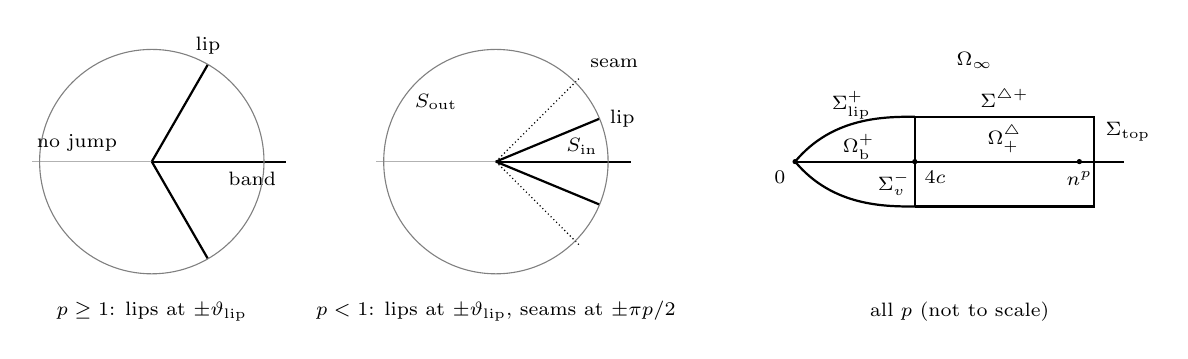
\begin{tikzpicture}[scale=0.95,>=Stealth,font=\scriptsize]
  % panel 1: p >= 1
  \begin{scope}
    \draw[gray!60] (-1.6,0)--(0,0);
    \draw[thick] (0,0)--(1.8,0) node[below left]{band};
    \draw[thick] (0,0)--(60:1.5) node[above]{lip};
    \draw[thick] (0,0)--(-60:1.5);
    \draw[gray] (0,0) circle (1.5);
    \node at (0,-2.0) {$p\ge1$: lips at $\pm\thlip$};
    \node at (-1.0,0.25) {no jump};
  \end{scope}
  % panel 2: p < 1
  \begin{scope}[xshift=4.6cm]
    \draw[gray!60] (-1.6,0)--(0,0);
    \draw[thick] (0,0)--(1.8,0);
    \draw[thick] (0,0)--(22.5:1.5) node[right]{lip};
    \draw[thick] (0,0)--(-22.5:1.5);
    \draw[densely dotted] (0,0)--(45:1.6) node[above right]{seam};
    \draw[densely dotted] (0,0)--(-45:1.6);
    \draw[gray] (0,0) circle (1.5);
    \node at (0,-2.0) {$p<1$: lips at $\pm\thlip$, seams at $\pm\pi p/2$};
    \node at (-0.8,0.8) {$\Sout$};
    \node at (1.15,0.2) {$\Sin$};
  \end{scope}
  % panel 3: global
  \begin{scope}[xshift=8.6cm,yshift=0cm]
    \draw[thick] (0,0)--(4.4,0);
    \draw[thick] (0,0) .. controls (0.5,0.6) and (1.2,0.6) .. (1.6,0.6);
    \draw[thick] (0,0) .. controls (0.5,-0.6) and (1.2,-0.6) .. (1.6,-0.6);
    \draw[thick] (1.6,-0.6)--(1.6,0.6);
    \draw[thick] (1.6,0.6)--(4.0,0.6)--(4.0,-0.6)--(1.6,-0.6);
    \fill (0,0) circle (1pt) node[below left]{$0$};
    \fill (1.6,0) circle (1pt) node[below right]{$4c$};
    \fill (3.8,0) circle (1pt) node[below]{$n^p$};
    \node at (0.85,0.2) {$\Ob^+$};
    \node at (2.8,0.3) {$\Osat_+$};
    \node at (0.75,0.75) {$\Sigma^+_{\mathrm{lip}}$};
    \node at (1.32,-0.3) {$\Sigma^-_v$};
    \node at (2.8,0.85) {$\Sigma^{\triangle+}$};
    \node at (4.45,0.4) {$\Sigma_{\mathrm{top}}$};
    \node at (2.4,1.35) {$\Oinf$};
    \node at (2.2,-2.0) {all $p$ (not to scale)};
  \end{scope}
\end{tikzpicture}
\caption{The contour near the hard edge for $p\ge1$ (the local pictures for $p>1$ and $p=1$ coincide) and for $p<1$,
and the whole contour. The lips are drawn at the default angles $\thlip=\pi/3$ and $\pi p/4$ (with $p=\frac12$); for
small $\vartheta$ they are rotated towards the band. The negative axis and, for $p<1$, the seams carry no jump of $V$
or $Q$. The seams are used only to construct the outer scalar (Appendix~\ref{app:outer}).}
\label{fig:geometry}
\end{figure}

\subsection{The transformations}\label{sec:frame-transf}
We now remove the poles, normalise at infinity and open the lens. The pattern is that of \S\ref{sec:tool-wlxz}(b);
since we work in a one-sided variable, we write every factor out. Put, in $\C_\pm$,
\begin{equation}\label{eq:upsilon}
  \upsilon_\pm:=\frac1{1-e^{\mp2i\theta}},\qquad\text{so that}\qquad \upsilon_\pm-1=e^{\mp2i\theta}\upsilon_\pm .
\end{equation}
By~\eqref{eq:imtheta}, $|e^{\mp2i\theta}|<1$ in $\C_\pm\cap\Zn$, so $\upsilon_\pm$ is analytic there. Define,
on $\Zn\cap\C_\pm$,
\begin{equation}\label{eq:LA}
  L_\pm:=\begin{pmatrix}1&\mp We^{\mp2i\theta}\upsilon_\pm\\0&1\end{pmatrix},\qquad
  A_\pm:=\begin{pmatrix}1&0\\\mp e^{2n\varphi}/W&1\end{pmatrix},\qquad
  A^\triangle_\pm:=\begin{pmatrix}1&0\\\mp1/(\upsilon_\pm W)&1\end{pmatrix}.
\end{equation}

\emph{Step 1: removal of the poles.} Let
\begin{equation}\label{eq:R}
  R:=U\ \text{in }\Oinf,\qquad R:=UL_\pm\ \text{in }\Ob^\pm,\qquad R:=UA^\triangle_\pm\,\upsilon_\pm^{\sigma_3}\ \text{in }\Osat_\pm .
\end{equation}
The restriction of $R$ to each of the four regions $\Ob^\pm$, $\Osat_\pm$ extends continuously to the real axis,
including the nodes. Near $X_k$ all factors are meromorphic, and $1-e^{\mp2i\theta}=\pm2i\theta'(X_k)
(z-X_k)(1+O(z-X_k))$ because $e^{2i\theta(X_k)}=1$. In $\Ob^\pm$ the entry $\mp We^{\mp2i\theta}\upsilon_\pm$ then has
the simple pole $W(X_k)/(2i\theta'(X_k)(z-X_k))=w(X_k)/(z-X_k)$, and $R_{j2}=U_{j2}-U_{j1}w(X_k)/(z-X_k)+O(1)$ is
regular by Lemma~\ref{lem:interp}. In $\Osat_\pm$, $\upsilon_\pm^{-1}$ vanishes simply at $X_k$, which removes the pole
of the second column; the first column is $\upsilon_\pm(U_{j1}\mp U_{j2}/(\upsilon_\pm W))$, and the bracket vanishes at
$X_k$ since $U_{j2}/(\upsilon_\pm W)\to\pm U_{j1}(X_k)$, so the first column is regular too.

\emph{Step 2: normalisation.} $T:=e^{-n\gamma_p\sigma_3}Re^{n\varphi\sigma_3}$.

\emph{Step 3: the lens.} $S:=TA_\pm$ in $\Ob^\pm$, and $S:=T$ elsewhere.

\emph{Step 4: the outer scalar.} Given a function $F$ with the properties~(a) and~(b) of
Definition~\ref{def:outer-admissible} below and its lens scalar $\tilde F$, let
\begin{equation}\label{eq:V}
  V:=C_\infty\,S\,\tilde F^{\sigma_3}\ \text{in }\Ob\cup\Osat,\qquad V:=C_\infty\,S\,F^{\sigma_3}\ \text{in }\Oinf,
\end{equation}
with a constant diagonal matrix $C_\infty$ fixed in Lemma~\ref{lem:normalisation}.

Composing the four steps, and using $\upsilon_\pm^{\sigma_3}\tilde F^{\sigma_3}=F^{\sigma_3}$ in $\Osat_\pm$
(definition~\eqref{eq:Ftilde} below),
\begin{equation}\label{eq:VM}
  V=C_\infty e^{-n\gamma_p\sigma_3}\,U\,M,\qquad
  M:=\begin{cases}e^{n\varphi\sigma_3}F^{\sigma_3}&\text{in }\Oinf,\\
  L_\pm e^{n\varphi\sigma_3}A_\pm\tilde F^{\sigma_3}&\text{in }\Ob^\pm,\\
  A^\triangle_\pm e^{n\varphi\sigma_3}F^{\sigma_3}&\text{in }\Osat_\pm.\end{cases}
\end{equation}
Since $U$ is analytic off the nodes, the jump of $V$ on any arc of $\Sigma$ away from the nodes is $M_-^{-1}M_+$.

In \cite{WLXZ} the saturated region is treated in two steps, by the factors $\Pi^{-\sigma_3}(\cdot)$ of
\cite[(3.10)--(3.11)]{WLXZ} and $V^\triangle_\pm$ of \cite[(4.12)--(4.13)]{WLXZ} (\S\ref{sec:tool-wlxz}(b)). Our factor
$A^\triangle_\pm\upsilon_\pm^{\sigma_3}$ combines them into one step. In $\Osat_-$ it carries a minus sign relative to
the literal product of the two factors; this is the sign of the factor $-V^\triangle_-$ that \cite[(4.12)]{WLXZ}
uses in the regions $\Omega^\triangle_{l,+}\cup\Omega^\triangle_{r,-}$, which lie in the second and fourth quadrants and
are therefore mapped into $\C_-$ by $z\mapsto z^2$. Without this sign, $V$ would have the constant jump $-I$ on the
saturated segment.

\subsection{Where the weight is evaluated}\label{sec:frame-where}
The following bookkeeping explains why an angle $\vartheta>0$ of any size suffices.

\begin{lemma}[Where the weight is evaluated]\label{lem:weightdomain}
The functions $w$, $W$, $r_n$ and $W_0$ (defined in~\eqref{eq:W0}) are evaluated only at points of $\Zn$.
Specifically, they are evaluated (a) in $\overline{\Ob\cup\Osat}\setminus\{0\}$, which contains every arc of $\Sigma$
except the top segment and the parts of the lips outside the lens; (b) on the lips and on the top segment; and (c) in
the sectors $\{|\arg z|\le\frac54\thlip\}\cap U(0,\delta)$ used in Section~\ref{sec:hardedge} and
Appendix~\ref{app:apriori}. The region $\Oinf$ never uses the weight: there $M=e^{n\varphi\sigma_3}F^{\sigma_3}$
contains neither $w$ nor $W$. Consequently $\xi(z)=\log t(z)$ always lies in
$\{\re\xi\ge-c_0,\ |\im\xi|\le\thw/p\}\subset S_\vartheta$.
\end{lemma}

\begin{proof}
By~\eqref{eq:VM}, $w$ and $W$ enter $V$ only in $\Ob\cup\Osat$, whose closure minus $\{0\}$ lies in $\Zn$
(\S\ref{sec:frame-contour}); the top segment has $|z|\le n^p+\delta'+h_0<e^{pc_0}n^p$ and $|\arg z|<\thw$. The
sectors used near $0$ lie in $\Zn$ because $\frac54\thlip<\thw$. For $z\in\Zn$, $\re\xi=\log n-\frac1p\log|z|>-c_0$
and $|\im\xi|=|\arg z|/p<\thw/p$.
\end{proof}

\begin{remark}[The angles]\label{rem:angles}
The angle $\vartheta$ of Definition~\ref{def:analytic} enters the proof only through $\thw\le p\vartheta$, and $\thw$
and $\thlip$ enter only through~\eqref{eq:angles}. The angle $\thlip$ can be taken as small as we wish because the
Bessel model admits rays at $\pm(\pi-\thlip)$ for every $\thlip\in(0,\pi)$ (\S\ref{sec:tool-bessel}(b)), and the lens
near $0$ is then the preimage of these rays. Every step that uses the angles needs only a fixed positive lower bound,
which \eqref{eq:angles} provides: the decay factors $\sin(\thlip/2)$ in~\eqref{eq:he-localisation} and
$\sin(\frac34\thlip/p)$ in Lemma~\ref{lem:supersmall}; the bound $\sin(\phi/p)\ge\frac2\pi\frac\phi p$
in~\eqref{eq:retvphi-zero}, which needs $\thw/p<\pi/2$; the separation $|x-z|\ge(x+|z|)/C$ for
$|\arg z|\ge\frac12\thlip$ in Lemma~\ref{lem:szego}(vi) and Appendix~\ref{app:apriori}; and the large-argument
expansions of the Bessel functions, which are used in the closed sector $|\arg2\zeta^{1/2}|\le\frac12(\pi-\thlip)$
(\S\ref{sec:he-model}). The order of choices is: $\vartheta$, then $\thw,\thlip$ by~\eqref{eq:thetaw}, then $\delta_1$,
then $\delta\le\delta_1$, which is also taken so small that the angle-dependent conditions in
Lemmas~\ref{lem:supersmall}(b), \ref{lem:lip-mismatch} and~\ref{lem:comparison-parametrix}(i) hold (they depend only on
$p$, $s$, $\ell$, $\thw$, $\thlip$, never on $n$), then $h_0$, $\eps$, $\delta'$, and $n_0$ last. Smaller angles make
the radii $\delta$, $h_0$, $\eps$ smaller and the threshold $n_0$ and the constants larger, but they do not change the
statements. The upper bounds in~\eqref{eq:angles} are what the construction needs: $\thw<\pi/2$ (convexity of the
sector $Z(r)$ in Lemma~\ref{lem:szego}, and $|y-z|\ge(|y|+|z|)/\sqrt2$ for $y<0$ in Lemma~\ref{lem:binetcut}),
$\thw<\pi p/2$ for $p<1$ (the lens must lie in the inner sector of the seam construction), and $\frac54\thlip<\thw$
(the sectors near $0$ in which the weight is used lie in $\Zn$). With the default angles ($\mathsf m=1$) the strip
needed is $|\im\xi|\le7\pi/(16p)$ for $p\ge1$ and $|\im\xi|\le3\pi/8$ for $p<1$; it is never necessary to continue
$\Lambda$ to the strip $|\im\xi|\le\pi/p$ that corresponds to the whole slit plane in $z$.
\end{remark}

\begin{lemma}[Potter bounds in the sector]\label{lem:pottersector}
For every $\eta>0$ there is $C_\eta$ such that:
\begin{enumerate}
\item[(i)] $|\Lambda(\xi)|\le C_\eta+\eta\re\xi$ for $\xi\in S_\vartheta$, $\re\xi\ge0$, and $|\Lambda|\le C$ on
  $S_\vartheta\cap\{\re\xi\le0\}$. Hence $|\ell(t)|^{\pm1}\le C_\eta|t|^\eta$ for $|\arg t|\le\vartheta$,
  $|t|\ge1$.
\item[(ii)] $|r_n(z)|^{\pm1}\le C_\eta n^{2\eta}(1+|z|^{-\eta/p})$ for $z\in\Zn$.
\item[(iii)] For $R\ge1$, $z\in\Zn$ with $|z|\le R$ and $x\in(0,R]$,
  \begin{gather*}
    |\log r_n(z)-\log r_n(x)|\le\frac{\eps_\Lambda(T)}p\bigl(|\arg z|+|\log(x/|z|)|\bigr),\\
    |\log r_n(z)|\le\frac{\eps_\Lambda(T)}p\bigl(|\arg z|+|\log|z||\bigr),
  \end{gather*}
  with $T:=\log n-\frac1p\log R$. Here $\log r_n=\Lambda(\xi)-\Lambda(\log n)$.
\end{enumerate}
\end{lemma}

\begin{proof}
(i) For $\re\xi\ge T_0$, integrate $\Lambda'$ along the horizontal segment from $T_0+i\im\xi$ to $\xi$:
$|\Lambda(\xi)-\Lambda(T_0+i\im\xi)|\le\eps_\Lambda(T_0)\re\xi$. Choose $T_0$ with $\eps_\Lambda(T_0)\le\eta$; $\Lambda$
is bounded on the compact set $S_\vartheta\cap\{0\le\re\xi\le T_0\}$ and, by hypothesis, on $\re\xi\le0$. Then
$|\ell(t)|^{\pm1}=e^{\pm\re\Lambda(\log t)}$.
(ii) $|r_n|^{\pm1}=|\ell(t)|^{\pm1}\ell(n)^{\mp1}$ with $|t|=n|z|^{-1/p}$; apply~(i) to both factors (for $|t|\le1$ use
the bound on $\re\xi\le0$).
(iii) Join $\xi(x)$ to $\xi(z)$ by the horizontal segment from $\log n-\frac1p\log x$ to $\log n-\frac1p\log|z|$
followed by the vertical segment to $\xi(z)$. Along this path $\re\xi\ge T$ and $|\im\xi|\le|\arg z|/p$, and its length
is $(|\log(x/|z|)|+|\arg z|)/p$. The second inequality is the case $x=1$, since $r_n(1)=1$.
\end{proof}

\subsection{\texorpdfstring{The outer scalar and the jumps of $V$}{The outer scalar and the jumps of V}}\label{sec:frame-outer}
Section~\ref{sec:outer} constructs, for each geometry, a function $F$ with the following properties. Put
$\nu_p:=\min(1/p,\frac12)$.

\begin{definition}[Admissible outer scalar]\label{def:outer-admissible}
A function $F=F_n$, defined for every $n\ge n_0$, is an \emph{admissible outer scalar} if it has the following five
properties for every $n\ge n_0$, where the constants $C$ in~(c) and~(d) do not depend on $n$.
\begin{enumerate}
\item[(a)] $F$ is analytic and zero-free in $\C\setminus[0,\infty)$ (in particular, it has no jump on $(-\infty,0)$),
  it has continuous boundary values on $(0,\infty)\setminus\{X_k\}$, and $F_+=F_-e^{2i\theta}$ on
  $(4c,\infty)\setminus\{X_k\}$.
\item[(b)] The \emph{lens scalar}
  \begin{equation}\label{eq:Ftilde}
    \tilde F:=(1-e^{\mp2i\theta})F=F/\upsilon_\pm\qquad\text{in }\C_\pm\cap\Zn
  \end{equation}
  extends to an analytic, zero-free function on $\Zn\setminus[4c,\infty)$, with $\tilde F_+=-\tilde F_-$ on
  $(4c,e^{pc_0}n^p)$. Thus $\tilde F^2$ is analytic and zero-free on $\Zn$, and so is the \emph{band factor}
  \begin{equation}\label{eq:Hn}
    H_n(z):=\frac1{(4c-z)\tilde F(z)^2}\qquad(z\in\Zn).
  \end{equation}
  Moreover $H_n>0$ on $(0,e^{pc_0}n^p)$, and $H_n(0^+):=\lim_{z\to0,\,z\in\Zn}H_n(z)$ exists in $(0,\infty)$.
\item[(c)] For $z\in\Zn$ with $|z|\le1$:
  $|\log H_n(z)-\log H_n(0^+)|\le C|z|^{\nu_p}$ and $|(\log H_n)'(z)|\le C|z|^{\nu_p-1}$.
\item[(d)] For $z\in\Zn$ with $|z|\ge1$: $|\log H_n(z)-\log H_n(0^+)|\le C\bigl(1+\log(1+|z|)\bigr)^2$.
\item[(e)] (For each fixed $n$.) $|F|^{\pm1}$ is bounded on $U(0,\delta)\setminus(\overline{\Ob}\cup[0,\infty))$, and
  $\tilde F^{\pm1}$ is bounded on $U(0,\delta)\cap\Ob$. There is $N_n$ with $|F(z)|^{\pm1}\le C_n|z|^{N_n}$ for
  $|z|\ge n^p+\delta'$, $z\notin\R$, and $F(iy)$ is bounded and bounded away from $0$ as $y\to\pm\infty$.
\end{enumerate}
\end{definition}

For such an $F$ the \emph{band weight} is
\begin{equation}\label{eq:W0}
  W_0:=\frac W{\tilde F^2}=\wn\,z^\alpha(4c-z)H_n(z)r_n(z)\quad\text{on }\Zn
\end{equation}
(Lemma~\ref{lem:bandweight}). On $(0,4c)$ it equals the constant $\wn$ times a positive function.

\begin{lemma}[Jumps of $V$]\label{lem:jumpsV}
Let $F$ have the properties~(a) and~(b) of Definition~\ref{def:outer-admissible}. Then $V$ is analytic in
$\C\setminus\Sigma$, has continuous boundary values on $\Sigma$ minus its vertices (including at the nodes), and
$V_+=V_-v_V$ with
\begin{enumerate}
\item[(a)] on the band $(0,4c)$: $v_V=\begin{pmatrix}0&W_0\\-1/W_0&0\end{pmatrix}$;
\item[(b)] on $\Sigma^\pm_{\mathrm{lip}}$ (oriented away from $0$), with $\iota_+=1$ and $\iota_-=0$:
  \[
    v_V=\begin{pmatrix}1&0\\e^{2n\varphi}/W_0&1\end{pmatrix}
    +\begin{pmatrix}\iota_\pm(\upsilon_\pm-1)&W_0e^{-2n\tvphi}\\(\upsilon_\pm-1)e^{2n\varphi}/W_0&\iota_\mp(\upsilon_\pm-1)\end{pmatrix};
  \]
\item[(c)] on $\Sigma_v^\pm$ (oriented away from the real axis): $v_V=\begin{pmatrix}1&-W_0e^{-2n\tvphi}\\0&1\end{pmatrix}$;
\item[(d)] on the saturated segment $(4c,n^p+\delta')$: $v_V=\begin{pmatrix}1&0\\e^{2n\tvphi}/W_0&1\end{pmatrix}$;
\item[(e)] on $\Sigma^{\triangle\pm}$ (oriented from left to right): $v_V=\begin{pmatrix}1&0\\\upsilon_\pm e^{2n\varphi}/W_0&1\end{pmatrix}$;
\item[(f)] on $\Sigma_{\mathrm{top}}\cap\C_\pm$ (oriented upwards): $v_V=\begin{pmatrix}1&0\\\mp\upsilon_\pm e^{2n\varphi}/W_0&1\end{pmatrix}$;
\item[(g)] there is no jump on $(-\infty,0)$ or on $(n^p+\delta',\infty)$.
\end{enumerate}
\end{lemma}

\begin{proof}
We compute $M_-^{-1}M_+$ from~\eqref{eq:VM} arc by arc, using the identities
\begin{equation}\label{eq:identities}
  e^{\mp2i\theta}e^{-2n\varphi}=e^{-2n\tvphi},\qquad F=\upsilon_\pm\tilde F,\qquad W/\tilde F^2=W_0\qquad\text{in }\C_\pm .
\end{equation}
For a diagonal matrix $D=\mathrm{diag}(d_1,d_2)$, conjugation $D^{-1}XD$ multiplies the $(1,2)$ entry by $d_2/d_1$ and
the $(2,1)$ entry by $d_1/d_2$.

(a) $L_-^{-1}L_+=\bigl(\begin{smallmatrix}1&W\\0&1\end{smallmatrix}\bigr)$: its $(1,2)$ entry is
$-W(e^{-2i\theta}\upsilon_++e^{2i\theta}\upsilon_-)=-W\bigl(\frac{e^{-2i\theta}}{1-e^{-2i\theta}}+\frac1{e^{-2i\theta}-1}\bigr)=W$.
Conjugating by $e^{n\varphi_\pm\sigma_3}$ and using $\varphi_-=-\varphi_+$ (Lemma~\ref{lem:gfunction}(i)) gives
$\bigl(\begin{smallmatrix}e^{2n\varphi_+}&W\\0&e^{2n\varphi_-}\end{smallmatrix}\bigr)$, and
\[
  A_-^{-1}\begin{pmatrix}e^{2n\varphi_+}&W\\0&e^{2n\varphi_-}\end{pmatrix}A_+=\begin{pmatrix}0&W\\-1/W&0\end{pmatrix}.
\]
Since $\tilde F$ has no jump on the band (Definition~\ref{def:outer-admissible}(b)), the final conjugation gives~(a)
by~\eqref{eq:identities}.

(b) Upper lip: the $+$ side is $\Oinf$, so $v_V=M_{\Ob}^{-1}M_{\Oinf}=\tilde F^{-\sigma_3}A_+^{-1}\bigl(e^{-n\varphi\sigma_3}
L_+^{-1}e^{n\varphi\sigma_3}\bigr)F^{\sigma_3}$. The bracket is $\bigl(\begin{smallmatrix}1&W\upsilon_+e^{-2n\tvphi}\\0&1
\end{smallmatrix}\bigr)$, and
\[
  A_+^{-1}\begin{pmatrix}1&W\upsilon_+e^{-2n\tvphi}\\0&1\end{pmatrix}=
  \begin{pmatrix}1&W\upsilon_+e^{-2n\tvphi}\\e^{2n\varphi}/W&\upsilon_+\end{pmatrix},
\]
because $1+\upsilon_+e^{2n\varphi}e^{-2n\tvphi}=1+\upsilon_+e^{-2i\theta}=\upsilon_+$. Conjugating with
$\tilde F^{-\sigma_3}(\cdot)F^{\sigma_3}$, $F=\upsilon_+\tilde F$, gives
$\bigl(\begin{smallmatrix}\upsilon_+&W_0e^{-2n\tvphi}\\\upsilon_+e^{2n\varphi}/W_0&1\end{smallmatrix}\bigr)$, which
is~(b). The lower lip (where the $+$ side is the lens) is the mirror computation and gives
$\bigl(\begin{smallmatrix}1&W_0e^{-2n\tvphi}\\\upsilon_-e^{2n\varphi}/W_0&\upsilon_-\end{smallmatrix}\bigr)$.

(c) Upper segment, $+$ side $=\Ob^+$: $v_V=M_{\Osat}^{-1}M_{\Ob}=F^{-\sigma_3}e^{-n\varphi\sigma_3}(A^\triangle_+)^{-1}L_+
e^{n\varphi\sigma_3}A_+\tilde F^{\sigma_3}$. One checks $(A^\triangle_+)^{-1}L_+=\bigl(\begin{smallmatrix}1&-We^{-2i\theta}
\upsilon_+\\1/(\upsilon_+W)&1-e^{-2i\theta}\end{smallmatrix}\bigr)$, and after the conjugation by $e^{n\varphi\sigma_3}$
and right multiplication by $A_+$ the $(2,1)$ entry vanishes and the diagonal becomes $(\upsilon_+,\upsilon_+^{-1})$; the
final conjugation with $F=\upsilon_+\tilde F$ removes the diagonal and gives~(c). The lower segment, whose $+$ side is
$\Osat_-$, is the mirror image.

(d) On $(4c,n^p+\delta')$ both sides lie in $\Osat$. Since $\upsilon_\pm^{-1}=1-e^{\mp2i\theta}$,
\[
  (A^\triangle_-)^{-1}A^\triangle_+=\begin{pmatrix}1&0\\-(\upsilon_+^{-1}+\upsilon_-^{-1})/W&1\end{pmatrix},\qquad
  \upsilon_+^{-1}+\upsilon_-^{-1}=2-2\cos2\theta=\upsilon_+^{-1}\upsilon_-^{-1}.
\]
Conjugating by $e^{n\varphi\sigma_3}F^{\sigma_3}$ with boundary values, the diagonal becomes
\[
  (e^{n(\varphi_+-\varphi_-)}F_+/F_-)^{\sigma_3}=(e^{-2i\theta}e^{2i\theta})^{\sigma_3}=I
\]
by Lemma~\ref{lem:gfunction}(i) and Definition~\ref{def:outer-admissible}(a), and the $(2,1)$ entry becomes
\[
  -e^{n(\varphi_++\varphi_-)}F_+F_-/(\upsilon_+\upsilon_-W)=-e^{2n\tvphi}\tilde F_+\tilde F_-/W .
\]
By Definition~\ref{def:outer-admissible}(b), $-\tilde F_+\tilde F_-=\tilde F^2$, which gives~(d).

(e), (f) Here $v_V=(F^{-\sigma_3}e^{-n\varphi\sigma_3})(A^\triangle_\pm)^{\pm1}(e^{n\varphi\sigma_3}F^{\sigma_3})$ with
the exponent fixed by the orientation, and the $(2,1)$ entry $\mp1/(\upsilon_\pm W)$ of $A^\triangle_\pm$ becomes
$\mp F^2e^{2n\varphi}/(\upsilon_\pm W)=\mp\upsilon_\pm e^{2n\varphi}/W_0$.

(g) On $(-\infty,0)$: $U$ has no jump, $e^{n\varphi}$ jumps by $e^{-2\pi in}=1$ (Lemma~\ref{lem:gfunction}(i)) and $F$
has no jump (Definition~\ref{def:outer-admissible}(a)). On $(n^p+\delta',\infty)$ there are no nodes, and
$M_-^{-1}M_+=(e^{n(\varphi_+-\varphi_-)}F_+/F_-)^{\sigma_3}=I$ as in~(d).

Continuity at the nodes: in~(a) and~(d) all entries are analytic across the real axis; together with Step~1 this shows
that $V$ has continuous boundary values there.
\end{proof}

% Section 5: the outer scalar; Szego functions, parametrices away from the hard edge; the properties of the frame.

\section{The outer scalar and the properties of the frame}\label{sec:outer}

The frame of Section~\ref{sec:frame} still lacks an admissible outer scalar $F$
(Definition~\ref{def:outer-admissible}), and constructing it is the only step of the Riemann--Hilbert analysis that
depends on the geometry. This section constructs $F$ and then carries out the steps common to all $p>0$: the Szeg\H{o} function of the band weight, the
normalisation at infinity, the estimates on the lips near the hard edge, and the Airy parametrix at the soft edge.
Proposition~\ref{prop:frame} collects the outcome; it is the only result of Sections~\ref{sec:frame}
and~\ref{sec:outer} used later. The standing assumptions of~\S\ref{sec:frame-standing} hold, so $s>1$ is arbitrary;
only item~(vii) of Proposition~\ref{prop:frame} requires $|\alpha|<1$.

The natural candidate for $F$ comes from Stirling's formula. The node masses carry the factor $1/\Gamma(t)$ through
$\Pi=\sin\theta/\theta'$, and
\[
  \tilde D(z):=e^{-j(t(z))},\qquad j(t):=\operatorname{Ln}\Gamma(t)-\bigl(t-\tfrac12\bigr)\ln t+t-\tfrac12\ln(2\pi),
\]
removes this growth. Here $j$ is Binet's function, $\operatorname{Ln}\Gamma$ is the branch analytic on
$\C\setminus(-\infty,0]$ and real on $(0,\infty)$, and $\ln t$ is principal; so
$\tilde D=\sqrt{2\pi}\,t^{t-1/2}e^{-t}/\Gamma(t)$, and this sign convention is used throughout. Then
\begin{equation}\label{eq:D}
  D:=\upsilon_\pm\tilde D=\frac{\tilde D}{1-e^{\mp2i\theta}}\quad\text{in }\C_\pm
\end{equation}
satisfies $D_+/D_-=(1-e^{2i\theta})/(1-e^{-2i\theta})=-e^{2i\theta}$ on $(0,\infty)$ off the nodes, and
$K(z):=(4c-z)^{-1/2}$ (principal branch, cut $[4c,\infty)$) supplies the missing factor $-1$, so that $DK$ has the
jump required in Definition~\ref{def:outer-admissible}(a).

The difficulty is the cut of $t(z)$ on $(-\infty,0)$, and how it is handled depends on how far the sector
$|\arg t|<\pi/p$ reaches (Table~\ref{tab:geometry}): for $p>1$ the jump of $DK$ on $(-\infty,0)$ is removed by a
Cauchy integral, the Binet-cut scalar $B$; at $p=1$ the reflection formula shows that $D$ has no jump there at all; for
$p<1$ the poles of $\Gamma(t)$ enter, and $D$ is used only in the inner sector $|\arg z|<\pi p/2$ and glued to an
elementary function outside along two seams. Lemma~\ref{lem:outer} states the result; the constructions for $p\ne1$
are in Appendix~\ref{app:outer}. The rest of the section (\S\ref{sec:outer-common}) is common to all geometries.

Two facts about $j$ are used in all three geometries. By DLMF~5.11.1 with the remainder bound of DLMF~\S5.11(ii), first
term $1/(12t)$ (\S\ref{sec:tool-dlmf}), for every $\phi<\pi$,
\begin{equation}\label{eq:binet-bound}
  |j(t)|\le\frac{\sec^2(\phi/2)}{12|t|},\qquad |j'(t)|\le\frac{C_\phi}{|t|^2}\qquad(|\arg t|\le\phi,\ |t|\ge1),
\end{equation}
the second by Cauchy's estimate on a disc of radius $|t|/C_\phi$ in a slightly larger sector. And for $|t|\le1$,
$\re t\ge0$, $t\ne0$, DLMF~5.5.1 gives $\operatorname{Ln}\Gamma(t)=\operatorname{Ln}\Gamma(1+t)-\ln t$, hence
\begin{equation}\label{eq:binet-small}
  j(t)=-\tfrac12\ln t-\tfrac12\ln(2\pi)+O(|t|\log(2/|t|))\qquad(t\to0,\ \re t\ge0).
\end{equation}

\subsection{The outer scalar}\label{sec:outer-scalar}

\begin{lemma}[Outer scalar]\label{lem:outer}
Define
\[
  F:=\begin{cases}DBK,&p>1,\ \text{with the Binet-cut scalar $B$ of~\eqref{eq:B}},\\
  DK,&p=1,\\
  DB_{\mathrm{in}}Ke^{\chi}\ \text{in }\Sin,\quad B_{\mathrm{out}}Ke^{\chi}\ \text{in }\Sout,&0<p<1,\ \text{with $B_{\mathrm{in}},B_{\mathrm{out}}$, $\chi$ of \S\ref{sec:outer-plt1}}.
  \end{cases}
\]
Then $F$ is an admissible outer scalar (Definition~\ref{def:outer-admissible}). The band factor is
$H_n=(\tilde DB)^{-2}$, $\tilde D^{-2}$, $(\tilde DB_{\mathrm{in}}e^{\chi})^{-2}$ respectively, with
$H_n(0^+)=B(0)^{-2}$, $1$, $e^{-2\chi(0)}$. At $p=1$,
\begin{equation}\label{eq:reflection}
  D(z)=\frac{e^{-j(t)}}{1-e^{\mp2\pi it}}=e^{j(-n/z)}\qquad(z\in\C_\pm),
\end{equation}
so $D$ extends analytically to $\C\setminus[0,\infty)$, it is real and positive on $(-\infty,0)$, and $H_n=e^{2j(n/z)}$.
\end{lemma}

\begin{table}[ht]
\centering\small
\renewcommand{\arraystretch}{1.25}
\begin{tabular}{@{}p{3.3cm}p{3.2cm}p{3.1cm}p{3.6cm}@{}}
\toprule
& $p>1$ & $p=1$ & $0<p<1$\tabularnewline
\midrule
\raggedright $\arg t$ on $\C\setminus(-\infty,0]$ & \raggedright $(-\pi/p,\pi/p)\subset(-\pi,\pi)$ & \raggedright $(-\pi,\pi)$, open & \raggedright wider than $(-\pi,\pi)$; poles of $\Gamma(t)$ on $\arg z=\pm\pi p$\tabularnewline
\raggedright where $\tilde D=e^{-j(t)}$ is used & \raggedright slit plane & \raggedright $|\arg z|<\thw$ & \raggedright inner sector $\Sin=\{|\arg z|<\pi p/2\}$\tabularnewline
\raggedright outer scalar $F$ (Lemma~\ref{lem:outer}) & \raggedright $DBK$, Binet-cut scalar $B$ & \raggedright $DK$, $D=e^{j(-n/z)}$, no cut & \raggedright $DB_{\mathrm{in}}Ke^{\chi}$ in $\Sin$, $B_{\mathrm{out}}Ke^{\chi}$ in $\Sout$\tabularnewline
\raggedright $|\log\frac{H_n(z)}{H_n(0^+)}|$ near $0$ & \raggedright $\le C|z|^{1/p}$ & \raggedright $\le C|z|$ & \raggedright $\le C|z|(1+\log\frac1{|z|})$\tabularnewline
\raggedright lip angle $\thlip$ (default); Bessel rays $\pm(\pi-\thlip)$ & \raggedright $\pi/3$ & \raggedright $\pi/3$ & \raggedright $\pi p/4$\tabularnewline
\raggedright angle $\thw$ (default; weight evaluated) & \raggedright $7\pi/16$ & \raggedright $7\pi/16$ & \raggedright $3\pi p/8$\tabularnewline
\raggedright super-small entries $|e^{\mp2i\theta}|$ on the rays $\arg z=\pm\thlip$ & \multicolumn{3}{p{10.3cm}}{\raggedright $e^{-2\pi n\sin(\thlip/p)|z|^{-1/p}}$; default angles: $e^{-2\pi n\sin(\frac{\pi}{3p})|z|^{-1/p}}$, $e^{-\sqrt3\pi n/|z|}$, $e^{-\sqrt2\pi n|z|^{-1/p}}$}\tabularnewline
\raggedright angle $\vartheta$ of $\ell$ & \raggedright any $\vartheta>0$; default angles if $\vartheta\ge\frac{7\pi}{16p}$ & \raggedright any $\vartheta>0$; default angles if $\vartheta\ge\frac{7\pi}{16}$ & \raggedright any $\vartheta>0$; default angles if $\vartheta\ge\frac{3\pi}{8}$\tabularnewline
\raggedright H\"older exponent $\nu_p$ (Definition~\ref{def:outer-admissible}) & \raggedright $\min(1/p,\frac12)$ & \raggedright $\frac12$ & \raggedright $\frac12$\tabularnewline
\raggedright classical quotient parametrix at $0$ & \raggedright used for pure powers in Section~\ref{sec:classical} & \raggedright fails (Remark~\ref{rem:quotient-p1}) & \raggedright not used\tabularnewline
\bottomrule
\end{tabular}
\caption{The ingredients of the Riemann--Hilbert analysis that depend on the geometry. Everything else in
Sections~\ref{sec:frame}--\ref{sec:extraction} is the same for all $p>0$. The angles $\thlip$ and $\thw$ are the
default values ($\mathsf m=1$ in~\eqref{eq:thetaw}); for smaller $\vartheta$ both are multiplied by
$\mathsf m=p\vartheta/\vartheta^0_{\mathrm w}<1$ (Remark~\ref{rem:angles}). In the row for $H_n$, only the weaker bound
$C|z|^{\nu_p}$ of Definition~\ref{def:outer-admissible}(c) is used.}
\label{tab:geometry}
\end{table}

\begin{proof}
For $p>1$ and $p<1$ this is Lemma~\ref{lem:binetcut}(iv), respectively Lemma~\ref{lem:seam}(iv). Let $p=1$, so $t=n/z$.

\emph{The identity~\eqref{eq:reflection}.} Let $z\in\C_+$, so $\arg t\in(-\pi,0)$ and $t\notin\R$. By DLMF~5.5.3
(\S\ref{sec:tool-dlmf}), $1/\Gamma(t)=\Gamma(1-t)\sin(\pi t)/\pi$, and $\sin(\pi t)/(1-e^{-2\pi it})=e^{i\pi t}/(2i)$.
Hence $D=\sqrt{2\pi}\,t^{t-1/2}e^{-t}\Gamma(1-t)e^{i\pi t}/(2\pi i)$. Put $u:=-t=-n/z$; then $\arg u=\arg t+\pi\in(0,\pi)$,
so $\ln u=\ln t+i\pi$ for the principal branches, and
$t^{t-1/2}e^{i\pi t}=\exp((t-\frac12)(\ln u-i\pi)+i\pi t)=e^{i\pi/2}u^{-u-1/2}$. So
$D=u^{-u-1/2}e^u\Gamma(1+u)/\sqrt{2\pi}$, and DLMF~5.5.1 ($\Gamma(1+u)=u\Gamma(u)$) together with the definition of $j$
gives $D=e^{j(u)}$. For $z\in\C_-$ the same computation with $\sin(\pi t)/(1-e^{2\pi it})=-e^{-i\pi t}/(2i)$ and
$\ln u=\ln t-i\pi$ gives the same result. Since $j$ is analytic on $\C\setminus(-\infty,0]$ and $u\in(-\infty,0]$
exactly when $z\in(0,\infty)$, $e^{j(-n/z)}$ is analytic on $\C\setminus[0,\infty)$; on $(-\infty,0)$, $u>0$ and $j(u)$
is real.

We check the properties (a)--(e) of Definition~\ref{def:outer-admissible}.

\emph{Property (a).} $F=DK$ is analytic and zero-free off $[0,\infty)$, and $F_+/F_-=(-e^{2i\theta})(-1)$ on
$(4c,\infty)$ off the nodes.

\emph{Property (b).} $\tilde F=F/\upsilon_\pm=\tilde DK$ with $\tilde D=e^{-j(t)}$ analytic and zero-free on
$\C\setminus(-\infty,0]$. So $H_n=\tilde D^{-2}=e^{2j(n/z)}>0$ on $(0,\infty)$, and $H_n(0^+)=1$.

\emph{Properties (c) and (d).} On $\Zn$, $|\arg t|=|\arg z|<\thw<\pi/2$. For $|z|\le1$, $|t|\ge n$
and~\eqref{eq:binet-bound} gives $|\log H_n|=2|j(t)|\le C|z|/n$ and $|(\log H_n)'|\le C/n$; since $\nu_1=\frac12$, this
is~(c). For $|z|\ge1$, $|t|\ge e^{-c_0}$ and $j(t)$ is bounded, which is~(d).

\emph{Property (e).} Fix $n$. Near $0$ outside the lens, $u=-n/z$ has $|u|\to\infty$ and
$|\arg u|=\pi-|\arg z|\le\pi-\frac34\thlip$, so $j(u)\to0$ by~\eqref{eq:binet-bound} and $D\to1$; $K$ is bounded. In the
lens $\tilde F=\tilde DK$ with $\tilde D\to1$. For $|z|\ge n+\delta'$ we have $|u|\le n/(n+\delta')<1$ and
$|1+u|\ge\delta'/(2n)$, and $D=u^{-u-1/2}e^u\Gamma(1+u)/\sqrt{2\pi}$ is bounded above and below by $C_n|z|^{\pm1}$. Along
$z=iy$, $D(iy)=(-iy/n)^{1/2}(2\pi)^{-1/2}(1+o(1))$ by~\eqref{eq:binet-small}, and $K(iy)=(-iy)^{-1/2}(1+o(1))$, so
$F(iy)\to(2\pi n)^{-1/2}$.
\end{proof}

At $p=1$ the cut of $D$ disappears, so this case is simpler than $p>1$; it does, however, break the classical
construction of the hard-edge parametrix (Remark~\ref{rem:quotient-p1}).

\subsection{\texorpdfstring{Common steps: Szeg\H{o} functions, normalisation, parametrices}{Common steps: Szego functions, normalisation, parametrices}}\label{sec:outer-common}
From now on $F$ is the outer scalar of Lemma~\ref{lem:outer}. Everything in this subsection uses only the properties
listed in Definition~\ref{def:outer-admissible}.

\emph{Szeg\H{o} functions.} Let $\mathcal R(z):=(z(z-4c))^{1/2}$, analytic off $[0,4c]$ with $\mathcal R(z)\sim z$ at
$\infty$, so that $\mathcal R_\pm(x)=\pm i\sqrt{x(4c-x)}$ on $(0,4c)$. Let $q$ be a function on $(0,4c)$ that is a
non-zero constant multiple of a positive function $q_0$ with $\log q_0\in L^1(\diff x/\sqrt{x(4c-x)})$, and fix a value
of the logarithm of the constant. Put
\begin{equation}\label{eq:szego}
  D_q(z):=\exp\Bigl(\frac{\mathcal R(z)}{2\pi}\int_0^{4c}\frac{\log q(x)}{\sqrt{x(4c-x)}}\frac{\diff x}{z-x}\Bigr),\qquad
  D_q(\infty)=\exp\Bigl(\frac1{2\pi}\int_0^{4c}\frac{\log q(x)\diff x}{\sqrt{x(4c-x)}}\Bigr).
\end{equation}
$D_q$ is analytic and zero-free off $[0,4c]$, $D_{q_1q_2}=D_{q_1}D_{q_2}$, and $D_q=q^{1/2}$ for a constant $q$. Where
$\log q_0$ is H\"older continuous, the Sokhotski--Plemelj formula and $\mathcal R_+=-\mathcal R_-$ give $D_{q,+}D_{q,-}=q$.

We shall estimate $D_q^2/q$ near the band by means of the following identity. Since
\[
  \frac1\pi\int_0^{4c}\frac{\diff x}{\sqrt{x(4c-x)}\,(z-x)}=\frac1{\mathcal R(z)}
\]
(the Stieltjes transform of the arcsine law, as in the proof of Lemma~\ref{lem:gfunction}), we have for every
$z\notin[0,4c]$ and every number $\mathfrak c$
\begin{equation}\label{eq:szego-repr}
  \log D_q(z)^2-\mathfrak c=\frac{\mathcal R(z)}\pi\int_0^{4c}\frac{(\log q(x)-\mathfrak c)\diff x}{\sqrt{x(4c-x)}\,(z-x)} .
\end{equation}
We use it with $\mathfrak c=\log q(z)$, the value of an analytic continuation of $\log q$. Put $\eta_*:=\min(1,2c)$ and
$Z(r):=\{z:\ 0<|z|<r,\ |\arg z|<\thw\}$.

\emph{The band weight and its Szeg\H{o} function.} Let $W_0$ be the band weight~\eqref{eq:W0}, $D_W:=D_{W_0}$ and
$D_\infty:=D_W(\infty)$. Writing $\Hc:=H_n/H_n(0^+)$,
\begin{equation}\label{eq:DW-factor}
  D_W=\bigl(\wn H_n(0^+)\bigr)^{1/2}\,D_{x^\alpha}\,D_{4c-x}\,D_{\Hc}\,D_{r_n}.
\end{equation}
All factors are defined: by Definition~\ref{def:outer-admissible}(c), (d), $\log\Hc$ is bounded on $(0,4c)$, and by
Lemma~\ref{lem:pottersector}(iii), $|\log r_n(x)|\le C\eps_\Lambda(T)(1+|\log x|)$. The constant $\wn H_n(0^+)$ cancels
in the ratio
\begin{equation}\label{eq:omega}
  \omega(z):=\frac{D_W(z)^2}{W_0(z)}
  =\frac{D_{x^\alpha}^2}{z^\alpha}\cdot\frac{D_{4c-x}^2}{4c-z}\cdot\frac{D_{\Hc}^2}{\Hc}\cdot\frac{D_{r_n}^2}{r_n},
\end{equation}
defined wherever $W_0$ is, i.e.\ on $\Zn\setminus[0,4c]$. In particular no bound on $H_n(0^+)$ is ever needed.

\begin{lemma}[Szeg\H{o} function estimates]\label{lem:szego}
The constants below depend only on $c$, the stated $\mathfrak M$, and $\eps_1$ in~(iv).
\begin{enumerate}
\item[(i)] Let $\Upsilon(z):=(z^{1/2}+(z-4c)^{1/2})^2=2z-4c+2\mathcal R(z)$, with principal roots. Then, with principal
  powers, $D_{x^\alpha}(z)^2=(4cz/\Upsilon(z))^\alpha$ and $D_{4c-x}(z)^2=4c(z-4c)/\Upsilon(z)$. $\Upsilon$ is analytic
  and zero-free off $[0,4c]$, with continuous non-zero boundary values, $\Upsilon(z)\sim4z$ at $\infty$,
  $\Upsilon(0)=-4c$, $\Upsilon(4c)=4c$, and $\Upsilon(z)=-4c(1+O(|z|^{1/2}))$ as $z\to0$. In particular
  $|D_{x^\alpha}(z)^2|\asymp|z|^\alpha$ and $|D_{4c-x}(z)^2|\asymp|z-4c|$ for $|z|\le8c$, $z\notin[0,4c]$.
\item[(ii)] (H\"older type at $0$.) Let $\nu\in(0,1]$, $\mathfrak M\ge0$, $\mathfrak c_0\in\C$. Suppose $\log q$
  continues analytically to $Z(\eta_*)$ and continuously to $(0,\eta_*)$, with $|\log q(z)-\mathfrak c_0|\le\mathfrak
  M|z|^\nu$ and $|(\log q)'(z)|\le\mathfrak M|z|^{\nu-1}$ there, and $|\log q(x)-\mathfrak c_0|\le\mathfrak
  M(1+|\log(4c-x)|)$ for $\frac12\eta_*\le x<4c$. Then for $z\in Z(\frac14\eta_*)\setminus(0,\infty)$,
  \[
    |\log D_q(z)^2-\log q(z)|\le C\mathfrak M|z|^{\min(\nu,1/2)}\log(2/|z|).
  \]
\item[(iii)] (Logarithmic type at $0$.) Suppose $\log q$ continues analytically to $Z(\eta_*)$ and continuously to
  $(0,\eta_*)$, with $|(\log q)'(z)|\le\mathfrak M/|z|$ there and $|\log q(x)-\log q(z)|\le\mathfrak
  M(1+|\log(x/|z|)|)$ for $z\in Z(\eta_*)$, $x\in(0,4c)$. Then $|\log D_q(z)^2-\log q(z)|\le C\mathfrak M$ for
  $z\in Z(\frac14\eta_*)\setminus(0,\infty)$.
\item[(iv)] (Near $4c$.) Suppose $\log q$ continues analytically to $\mathbb D(4c,2\eps_1)$, with $|\log q-\mathfrak
  c_1|\le\mathfrak M$ there and $|\log q(x)-\mathfrak c_1|\le\mathfrak M(1+|\log x|)$ on $(0,4c)$. Then $|\log
  D_q(z)^2-\log q(z)|\le C\mathfrak M\min(1,|z-4c|^{1/2})$ for $z\in \mathbb D(4c,\eps_1)\setminus[0,4c]$.
\item[(v)] (Away from the band.) If $|\log q(x)-\mathfrak c_1|\le\mathfrak M(1+|\log x|+|\log(4c-x)|)$ on $(0,4c)$,
  then $|\log D_q(z)^2-\mathfrak c_1|\le C_d\mathfrak M$ for $\mathrm{dist}(z,[0,4c])\ge d$.
\item[(vi)] (The band weight.) For $n\ge n_0$, with $C$ independent of $n$:
(a) $|\omega(z)|^{\pm1}\le C$ for $z\in Z(\frac14\eta_*)\setminus(0,\infty)$, in particular on the lips in $\mathbb D(0,\delta)$;
(b) in $\mathbb D(4c,2\eps)$,
\begin{equation}\label{eq:omega-4c}
  -\omega=\frac{4c}{\Upsilon}\,e^{L_1},\qquad L_1:=\log\frac{D_{q_1}^2}{q_1},\quad q_1:=x^\alpha\Hc r_n ,
\end{equation}
where $L_1$ is given by~\eqref{eq:szego-repr} with $\mathfrak c=\log q_1(z)$; $L_1$ is analytic in
$\mathbb D(4c,2\eps)\setminus[0,4c]$, real on $(4c,4c+2\eps)$, satisfies $L_{1,+}+L_{1,-}=0$ on $(4c-2\eps,4c)$ and
$|L_1(z)|\le C\min(1,|z-4c|^{1/2})$; in particular $|\omega(z)|^{\pm1}\le C$ there;
(c) $|\log\omega(z)|\le C_d\bigl(1+\log(1+|z|)\bigr)^2$ for $z\in\Zn$ with $\mathrm{dist}(z,[0,4c])\ge d$.
Moreover, for each fixed $n$, $|D_W(z)|^{\pm1}\le C_{n,\eta}|z|^{\pm\alpha/2-\eta}$ for every $\eta>0$ and
$0<|z|<\frac14\eta_*$, $z\notin[0,\infty)$.
\end{enumerate}
\end{lemma}

\begin{proof}
Part~(i) identifies two explicit functions with the right jumps. Parts~(ii)--(v) use the
representation~\eqref{eq:szego-repr} and a splitting of $(0,4c)$ into the near zone $|x-z|<\frac12|z|$ (or a
neighbourhood of $4c$) and the rest. Part~(vi) applies (i)--(v) to the four factors of~\eqref{eq:omega}.

(i) Write $\Upsilon=z(1+\mathfrak r)^2$ with $\mathfrak r:=\mathcal R(z)/z=\sqrt{1-4c/z}$, which has $\re\mathfrak r>0$
off $[0,4c]$. Then $4cz/\Upsilon=4c/(1+\mathfrak r)^2$ and $4c(z-4c)/\Upsilon=4c\,(\mathfrak r/(1+\mathfrak r))^2$;
both $1/(1+\mathfrak r)$ and $\mathfrak r/(1+\mathfrak r)$ lie in the disc $|\cdot-\frac12|<\frac12$, so their squares
avoid $(-\infty,0]$ and the principal powers are analytic off $[0,4c]$. On the band,
$\Upsilon_\pm=(\sqrt x\pm i\sqrt{4c-x})^2$, so $\Upsilon_+\Upsilon_-=16c^2$, the two boundary values of each expression
are complex conjugates, and the product of their principal powers is $x^{2\alpha}$, respectively $(4c-x)^2$. The
expressions tend to $c$ at $\infty$. Hence they are the Szeg\H{o} functions squared (the quotient of two functions with
the same jump, bounded at $\infty$ and of at most logarithmic growth at $0$ and $4c$, is constant). The values and the
expansion of $\Upsilon$ at $0$ and $4c$ are read off from $\Upsilon=(z^{1/2}+(z-4c)^{1/2})^2$.

(ii) Fix $z\in Z(\frac14\eta_*)\setminus(0,\infty)$ and use~\eqref{eq:szego-repr} with $\mathfrak c=\log q(z)$; here
$|\mathcal R(z)|\le C|z|^{1/2}$. Split $(0,4c)$ into $\mathcal U_z:=\{x:|x-z|<\frac12|z|\}$ and the rest. For
$x\in\mathcal U_z$ the segment $[x,z]$ lies in $Z(\eta_*)$ (the sector is convex since $\thw<\pi/2$) and at distance
$\ge\frac12|z|$ from $0$, so $|\log q(x)-\log q(z)|\le\mathfrak M(|z|/2)^{\nu-1}|x-z|$, and the contribution is at most
$C|z|^{1/2}\mathfrak M|z|^{\nu-1}\int_{\mathcal U_z}x^{-1/2}\diff x\le C\mathfrak M|z|^\nu$. Off $\mathcal U_z$,
$|x-z|\ge\frac18(x+|z|)$ (if $x\le3|z|$ then $|x-z|\ge\frac12|z|$; otherwise $|x-z|\ge x-|z|\ge\frac12x$). On
$(0,\frac12\eta_*)$ we have $|\log q(x)-\log q(z)|\le\mathfrak M(x^\nu+|z|^\nu)$, and
\[
  |z|^{1/2}\int_0^{\eta_*/2}\frac{\mathfrak M(x^\nu+|z|^\nu)\diff x}{x^{1/2}(x+|z|)}\le C\mathfrak M|z|^{\min(\nu,1/2)}\log(2/|z|),
\]
by the substitution $x=|z|u$: the term $|z|^\nu$ gives $C\mathfrak M|z|^\nu$; the term $x^\nu$ gives $C\mathfrak
M|z|^\nu$ if $\nu<\frac12$, $C\mathfrak M|z|^{1/2}\log(2/|z|)$ if $\nu=\frac12$, and $C\mathfrak M|z|^{1/2}$ if
$\nu>\frac12$. On $[\frac12\eta_*,4c)$, $|x-z|\ge\frac14\eta_*$ and
$\int(1+|\log(4c-x)|)(4c-x)^{-1/2}\diff x<\infty$ give $C\mathfrak M|z|^{1/2}$.

(iii) The same splitting. On $\mathcal U_z$ the derivative bound gives $|\log q(x)-\log q(z)|\le2\mathfrak M|x-z|/|z|$
and a contribution $C\mathfrak M$. Off $\mathcal U_z$ the contribution is at most
$C\mathfrak M|z|^{1/2}\int_0^{4c}\frac{(1+|\log(x/|z|)|)\diff x}{\sqrt{x(4c-x)}\,(x+|z|)}$, and the substitution
$x=|z|u$ bounds the part $x\le2c$ by $C\mathfrak M\int_0^\infty(1+|\log u|)u^{-1/2}(1+u)^{-1}\diff u$; the part $x\ge2c$
is $O(\mathfrak M|z|^{1/2}\log(2/|z|))$.

(iv) By Cauchy's estimate $|(\log q)'|\le 2\mathfrak M/\eps_1$ on $\mathbb D(4c,\frac32\eps_1)$. For
$x\in(4c-\frac32\eps_1,4c)$ and $z\in \mathbb D(4c,\eps_1)$, $|\log q(x)-\log q(z)|\le C\mathfrak M|x-z|$, which cancels the
kernel's singularity, and $\int(4c-x)^{-1/2}\diff x<\infty$. For $x\le4c-\frac32\eps_1$, $|z-x|\ge\frac12\eps_1$ and
the integrand is $\le C\mathfrak M(1+|\log x|)x^{-1/2}$. So the integral in~\eqref{eq:szego-repr} is at most
$C\mathfrak M$, and the prefactor satisfies $|\mathcal R(z)|\le C\min(1,|z-4c|^{1/2})$.

(v) In~\eqref{eq:szego-repr} with $\mathfrak c=\mathfrak c_1$, $|\mathcal R(z)/(z-x)|\le C_d$ for all $x\in[0,4c]$ when
$\mathrm{dist}(z,[0,4c])\ge d$, and the remaining integral is finite.

(vi)(a) Use the four factors of~\eqref{eq:omega}. The first two are bounded above and below by~(i), since $z^\alpha$
and $(4cz/\Upsilon)^\alpha$ differ by a bounded factor $(4c/\Upsilon)^\alpha e^{2\pi ik\alpha}$. The third is bounded
by~(ii) with $q=\Hc$, $\mathfrak c_0=0$, $\nu=\nu_p$ and $\mathfrak M=C$ from
Definition~\ref{def:outer-admissible}(c), (d). The fourth is bounded by~(iii) with $q=r_n$: by
Lemma~\ref{lem:pottersector}(iii) with $R=\max(4c,1)$, the hypotheses hold with
$\mathfrak M=C\eps_\Lambda(\log n-\frac1p\log\max(4c,1))\le C$, and $|(\log r_n)'(z)|=|\Lambda'(\xi)|/(p|z|)$.
(b) By~(i), $D_{4c-x}^2/(4c-z)=-4c/\Upsilon$, and the three other factors of~\eqref{eq:omega} combine, by
multiplicativity, into $D_{q_1}^2/q_1$; this is~\eqref{eq:omega-4c}. Near $4c$, $\Hc$ and $r_n$ are analytic and
positive on the real axis, with $|\log\Hc|\le C$ and $|\log r_n|\le C$ (Definition~\ref{def:outer-admissible}(d) and
Lemma~\ref{lem:pottersector}(iii)), so~(iv) applies to $q_1$ with $\mathfrak M=C$. The boundary values of the exponent
in~\eqref{eq:szego} add up to $\log q_1$ on the band (this is $D_{q_1,+}D_{q_1,-}=q_1$), so
$L_{1,+}+L_{1,-}=2\log q_1-2\log q_1=0$; and $L_1$ is real on $(4c,4c+2\eps)$ because $D_{q_1}$ and $q_1$ are positive
there.
(c) (v) with $q=W_0/(\wn H_n(0^+))$ bounds $\log D_W^2-\log(\wn H_n(0^+))$, and
$|\log(W_0(z)/(\wn H_n(0^+)))|\le C(1+\log(1+|z|))^2$ on $\Zn$ by Definition~\ref{def:outer-admissible}(c), (d) and
Lemma~\ref{lem:pottersector}(iii) with $R=e^{pc_0}n^p$ (here $|\log r_n(z)|\le\frac1p\eps_\Lambda(-c_0)(\thw+|\log|z||)$).
For the last claim, fix $n$ and $\eta>0$. By Lemma~\ref{lem:pottersector}(i),
$|\log r_n(x)|\le C_{n,\eta}+\eta|\log x|$ for $x\in(0,4c)$, and $|r_n(z)|^{\pm1}\le C_{n,\eta}|z|^{-\eta}$ for
$z\in\Zn$. For $|\arg z|<\thw$ the claim follows from~(a) and $|W_0|\asymp|z|^\alpha|r_n|$. For
$|\arg z|\ge\frac12\thlip$ we have $|x-z|\ge(x+|z|)/C$ for $x>0$, and~\eqref{eq:szego-repr} with $\mathfrak c=0$ gives
$|\log D_{\Hc}(z)|\le C$ and
\[
  |\log D_{r_n}(z)^2|\le C|z|^{1/2}\int_0^{4c}\frac{C_{n,\eta}+\eta|\log x|}{\sqrt{x(4c-x)}(x+|z|)}\diff x\le C_{n,\eta}+C\eta\log\frac1{|z|};
\]
together with~(i) for $D_{x^\alpha}$ and $D_{4c-x}$ this gives the claim (after renaming $\eta$).
\end{proof}

\emph{The global parametrix.} Let $a(z):=((z-4c)/z)^{1/4}$, analytic off $[0,4c]$ with $a(\infty)=1$, and
\begin{equation}\label{eq:Pinf0}
  P^\infty_0(z):=\begin{pmatrix}\frac{a+a^{-1}}2&\frac{a-a^{-1}}{2i}\\[1mm]-\frac{a-a^{-1}}{2i}&\frac{a+a^{-1}}2\end{pmatrix},\qquad
  P^\infty:=D_\infty^{\sigma_3}P^\infty_0D_W^{-\sigma_3}.
\end{equation}
Then $\det P^\infty_0=1$, $P^\infty_{0,+}=P^\infty_{0,-}J$ on $(0,4c)$ with
$J=\bigl(\begin{smallmatrix}0&1\\-1&0\end{smallmatrix}\bigr)$ (because $a_+=ia_-$ there), and $P^\infty_0(z)=I+O(1/z)$.
Since $|a(z)|^{\pm1}=|z-4c|^{\pm1/4}|z|^{\mp1/4}$,
\begin{equation}\label{eq:Pinf0-bound}
  |P^\infty_0(z)|\le C|z|^{-1/4}|z-4c|^{-1/4}(1+|z|)^{1/2}.
\end{equation}
As $D_{W,+}D_{W,-}=W_0$, $P^\infty$ has the band jump of $V$ (Lemma~\ref{lem:jumpsV}(a)). We put
\begin{equation}\label{eq:Q}
  Q:=D_\infty^{-\sigma_3}VD_W^{\sigma_3};
\end{equation}
in the frame of $Q$ the global parametrix is $P^\infty_0$, which does not involve the weight. A matrix $X$ in the frame
of $V$ corresponds to $D_\infty^{-\sigma_3}XD_W^{\sigma_3}$ in the frame of $Q$.

\begin{lemma}[Normalisation at infinity]\label{lem:normalisation}
Let $\mathsf h_\infty(z):=F(z)^{-1}e^{n(g(z)-\Log z)}$ for $|z|>n^p+\delta'$, $z\notin\R$. Then $\mathsf h_\infty$
extends to an analytic function on $\{|z|>n^p+\delta'\}\cup\{\infty\}$ with $\mathsf h_\infty(\infty)\ne0$. With
$C_\infty:=\mathsf h_\infty(\infty)^{\sigma_3}$ in~\eqref{eq:V}, $V(z)=I+O(1/z)$ and $Q(z)=I+O(1/z)$ as $z\to\infty$,
and for $|z|>n^p+\delta'+h_0$
\begin{equation}\label{eq:Q-at-infinity}
  Q(z)=k_\infty^{-\sigma_3}\bigl(U(z)z^{-n\sigma_3}\bigr)k(z)^{\sigma_3},\qquad k:=\frac{e^{n\gamma_p}D_W}{\mathsf h_\infty},
\end{equation}
where $k$ is analytic at $\infty$ with $k_\infty:=k(\infty)=e^{n\gamma_p}D_\infty/\mathsf h_\infty(\infty)\ne0$.
\end{lemma}

\begin{proof}
On $(-\infty,-n^p-\delta')$, $g$ and $\Log z$ both jump by $2\pi i$ and $F$ has no jump
(Definition~\ref{def:outer-admissible}(a)). On $(n^p+\delta',\infty)$, $e^{n(g-\Log z)}$ jumps by
$e^{2\pi in\mu^*((x,\infty))}=e^{2i\theta}$ (Lemma~\ref{lem:gfunction}(i)) and so does $F$. So $\mathsf h_\infty$ has
continuous boundary values that agree, and is analytic in $\{|z|>n^p+\delta'\}$ by Morera's theorem. By
Lemma~\ref{lem:gfunction}(ii) and Definition~\ref{def:outer-admissible}(e), $|\mathsf h_\infty(z)|\le C_n|z|^{N_n}$, so
$\infty$ is at most a pole; since $\mathsf h_\infty(iy)$ is bounded and bounded away from $0$ as $y\to\pm\infty$, it is
a removable singularity and $\mathsf h_\infty(\infty)\ne0$.

In $\Oinf$, by~\eqref{eq:VM}, $V=C_\infty e^{-n\gamma_p\sigma_3}(Uz^{-n\sigma_3})(z^ne^{n\varphi}F)^{\sigma_3}$, and
$z^ne^{n\varphi}F=e^{n\gamma_p}e^{-n(g-\Log z)}F=e^{n\gamma_p}/\mathsf h_\infty$. Hence
$V=\mathsf h_\infty(\infty)^{\sigma_3}e^{-n\gamma_p\sigma_3}(Uz^{-n\sigma_3})e^{n\gamma_p\sigma_3}\mathsf h_\infty^{-\sigma_3}=I+O(1/z)$,
by Lemma~\ref{lem:interp}. Multiplying by $D_\infty^{-\sigma_3}$ on the left and $D_W^{\sigma_3}$ on the right gives
\eqref{eq:Q-at-infinity}, and $D_W(z)/D_\infty=1+O(1/z)$ gives $Q=I+O(1/z)$; $D_W$ is analytic at $\infty$ because the
exponent in~\eqref{eq:szego} is.
\end{proof}

\begin{lemma}[Lip exponentials and super-small entries]\label{lem:supersmall}
Let $s_p:=\sin(\frac34\thlip/p)>0$. For $n\ge n_0$ and $z\in\Sigma^\pm_{\mathrm{lip}}\cap \mathbb D(0,\delta)$:
\begin{enumerate}
\item[(a)] $|\upsilon_\pm(z)-1|\le2\exp(-2\pi s_pn|z|^{-1/p})$;
\item[(b)] $|e^{-2n\tvphi(z)}|\le\exp(-\pi s_pn|z|^{-1/p})$;
\item[(c)] $|e^{2n\varphi(z)}|\le\exp\bigl(-2\sin(\thlip/2)\,n|f(z)|^{1/2}\bigr)\le e^{-n|z|^{1/2}/C}$.
\end{enumerate}
\end{lemma}

\begin{proof}
On these lips $\frac34\thlip\le|\arg z|\le\frac54\thlip$ (Lemma~\ref{lem:lips}), and $\frac54\thlip/p<\pi/2$ in all
cases, so $\sin(|\arg z|/p)\ge s_p$. (a) follows from~\eqref{eq:imtheta} and
$|\upsilon_\pm-1|=|e^{\mp2i\theta}|/|1-e^{\mp2i\theta}|$.
(b) $e^{-2n\tvphi}=e^{-2n\varphi}e^{\mp2i\theta}$ and $|\re\varphi|\le C|z|^{1/2}$ (Lemma~\ref{lem:signs}(iii)), so
$|e^{-2n\tvphi}|\le\exp(2Cn|z|^{1/2}-2\pi s_pn|z|^{-1/p})$, and $2C|z|^{1/2}\le\pi s_p|z|^{-1/p}$ for $|z|\le\delta$
small.
(c) By Lemma~\ref{lem:signs}(iii), $\re\varphi=-2\re f^{1/2}$, and on the lip $\arg f=\mp(\pi-\thlip)$, so
$\re f^{1/2}=|f|^{1/2}\sin(\thlip/2)$; finally $|f(z)|\ge|z|/C$ on $\mathbb D(0,\delta)$.
\end{proof}

\emph{The soft edge.} In $\mathbb D(4c,\eps)$ the jumps of $Q$ are, by Lemma~\ref{lem:jumpsV}(a), (c), (d) and the conjugation
by $D_W^{\sigma_3}$,
\begin{equation}\label{eq:jumps-4c}
  J\ \text{on }(4c-\eps,4c),\qquad
  \begin{pmatrix}1&0\\\omega e^{2n\tvphi}&1\end{pmatrix}\ \text{on }(4c,4c+\eps),\qquad
  \begin{pmatrix}1&-\omega^{-1}e^{-2n\tvphi}\\0&1\end{pmatrix}\ \text{on }\Sigma^\pm_v\cap \mathbb D(4c,\eps),
\end{equation}
the first two oriented from left to right and the last away from the real axis. This is the jump structure of
\cite[(6.4)]{WLXZ}. We construct the local solution from Airy functions, in our variable and with our orientations,
following the pattern of \cite[(6.10)--(6.12)]{WLXZ} (\S\ref{sec:tool-wlxz}(c)); the facts about $\mathrm{Ai}$ that we
use are those listed in \S\ref{sec:tool-dlmf}.

Let $\mathsf q:=e^{2\pi i/3}$ and define the vector functions
\[
  y_0(\zeta):=\begin{pmatrix}\mathrm{Ai}(\zeta)\\\mathrm{Ai}'(\zeta)\end{pmatrix},\qquad
  y_\pm(\zeta):=\begin{pmatrix}\mathrm{Ai}(\mathsf q^{\mp1}\zeta)\\\mathsf q^{\mp1}\mathrm{Ai}'(\mathsf q^{\mp1}\zeta)\end{pmatrix}.
\]
By DLMF~9.2.12 and its derivative, $y_0+\mathsf q^{-1}y_++\mathsf q\,y_-=0$. With
$k_{\mathrm{Ai}}:=\sqrt{2\pi}\,e^{i\pi/12}$ and $M=\frac1{\sqrt2}\bigl(\begin{smallmatrix}1&i\\i&1\end{smallmatrix}\bigr)$
(the matrix of \S\ref{sec:tool-bessel}(c)), put
\begin{equation}\label{eq:airy-model}
\begin{aligned}
  \Psi^{\mathrm I}&:=k_{\mathrm{Ai}}e^{-i\pi\sigma_3/4}\bigl(y_+,\ \mathsf q\,y_0\bigr),&
  \Psi^{\mathrm{II}}&:=k_{\mathrm{Ai}}e^{-i\pi\sigma_3/4}\bigl(y_+,\ -\mathsf q^{-1}y_-\bigr),\\
  \Psi^{\mathrm{III}}&:=k_{\mathrm{Ai}}e^{-i\pi\sigma_3/4}\bigl(-\mathsf q^{-1}y_-,\ -y_+\bigr),&
  \Psi^{\mathrm{IV}}&:=k_{\mathrm{Ai}}e^{-i\pi\sigma_3/4}\bigl(-\mathsf q^{-1}y_-,\ \mathsf q\,y_0\bigr).
\end{aligned}
\end{equation}
These are entire matrix functions of $\zeta$, independent of $n$. The relation $y_0+\mathsf q^{-1}y_++\mathsf qy_-=0$
gives
\begin{equation}\label{eq:airy-relations}
  \Psi^{\mathrm{II}}=\Psi^{\mathrm I}\begin{pmatrix}1&1\\0&1\end{pmatrix},\quad
  \Psi^{\mathrm{II}}=\Psi^{\mathrm{III}}J,\quad
  \Psi^{\mathrm{IV}}=\Psi^{\mathrm{III}}\begin{pmatrix}1&1\\0&1\end{pmatrix},\quad
  \Psi^{\mathrm I}=\Psi^{\mathrm{IV}}\begin{pmatrix}1&0\\-1&1\end{pmatrix},
\end{equation}
and $\det\Psi^{\mathrm I}=-k_{\mathrm{Ai}}^2\mathsf q\,\mathcal W\{\mathrm{Ai}(\zeta),\mathrm{Ai}(\mathsf q^{-1}\zeta)\}=
-2\pi e^{i\pi/6}\mathsf q\,e^{i\pi/6}/(2\pi)=1$ by DLMF~9.2.8, hence $\det\Psi^j\equiv1$ for all four. Let
$\mathcal S_{\mathrm I}:=\{0\le\arg\zeta\le\frac{7\pi}{12}\}$, $\mathcal S_{\mathrm{II}}:=\{\frac{5\pi}{12}\le\arg\zeta\le\pi\}$
and $\mathcal S_{\mathrm{III}},\mathcal S_{\mathrm{IV}}$ their mirror images (with $\arg\zeta=\pm\pi$ meaning the boundary
value from $\C_\pm$). Then, uniformly for $\zeta\in\mathcal S_j$, $|\zeta|\ge1$,
\begin{equation}\label{eq:airy-infty}
  \Psi^j(\zeta)=\zeta^{-\sigma_3/4}\bigl(M+O(|\zeta|^{-3/2})\bigr)e^{\frac23\zeta^{3/2}\sigma_3}.
\end{equation}
This holds because in each $\mathcal S_j$ the three arguments $\zeta$, $\mathsf q^{\pm1}\zeta$ that occur have
$|\mathrm{ph}|\le\frac{11\pi}{12}$, so the Airy asymptotics of \S\ref{sec:tool-dlmf} apply with relative errors
$O(|\zeta|^{-3/2})$. For instance, for $\zeta$ in $\mathcal S_{\mathrm I}\cup\mathcal S_{\mathrm{II}}$ we have
$(\mathsf q^{-1}\zeta)^{1/4}=e^{-i\pi/6}\zeta^{1/4}$ and $\frac23(\mathsf q^{-1}\zeta)^{3/2}=-\frac23\zeta^{3/2}$, so,
entrywise with relative errors $O(|\zeta|^{-3/2})$,
$y_+=\frac{1}{2\sqrt\pi}e^{\frac23\zeta^{3/2}}\zeta^{-\sigma_3/4}
\bigl(\begin{smallmatrix}e^{i\pi/6}\\e^{i\pi/6}\end{smallmatrix}\bigr)$ and
$y_0=\frac{1}{2\sqrt\pi}e^{-\frac23\zeta^{3/2}}\zeta^{-\sigma_3/4}\bigl(\begin{smallmatrix}1\\-1\end{smallmatrix}\bigr)$;
and
$k_{\mathrm{Ai}}e^{-i\pi\sigma_3/4}\frac1{2\sqrt\pi}\bigl(\begin{smallmatrix}e^{i\pi/6}&\mathsf q\\e^{i\pi/6}&-\mathsf q\end{smallmatrix}\bigr)=M$.
The other columns and sectors are the same computation with $(\mathsf q\zeta)^{1/4}=e^{-i\pi/3}\zeta^{1/4}$,
$(\mathsf q\zeta)^{3/2}=\zeta^{3/2}$ in $\mathcal S_{\mathrm{II}}$, and the mirror relations in
$\mathcal S_{\mathrm{III}}\cup\mathcal S_{\mathrm{IV}}$.

The disc $\mathbb D(4c,\eps)$ minus the contour has four components: $\Osat_+\cap \mathbb D(4c,\eps)$, $\Ob^+\cap \mathbb D(4c,\eps)$,
$\Ob^-\cap \mathbb D(4c,\eps)$, $\Osat_-\cap \mathbb D(4c,\eps)$; we label them I, II, III, IV. With $f_r$ of
Lemma~\ref{lem:signs}(iv) put $\zeta:=n^{2/3}f_r(z)$ and $\Psi_r(\zeta):=\Psi^j(\zeta)$ for $z$ in component $j$. By
Lemma~\ref{lem:signs}(iv), $|\arg f_r(z)-\arg(z-4c)|\le\frac\pi{12}$, so $\zeta\in\mathcal S_j$ when $z$ is in
component $j$. By Lemma~\ref{lem:szego}(vi)(b) let
\begin{equation}\label{eq:omega-root}
  (-\omega)^{1/2}:=\frac{2\sqrt c}{z^{1/2}+(z-4c)^{1/2}}\,e^{L_1/2}\qquad(z\in \mathbb D(4c,2\eps)\setminus[0,4c]),
\end{equation}
a square root of $-\omega$ (as $4c/\Upsilon=(2\sqrt c/(z^{1/2}+(z-4c)^{1/2}))^2$). It is analytic in
$\mathbb D(4c,2\eps)\setminus(4c-2\eps,4c]$, positive on $(4c,4c+2\eps)$, bounded above and below uniformly in $n$, and its
boundary values on the band satisfy
\begin{equation}\label{eq:omega-root-band}
  (-\omega)^{1/2}_+(-\omega)^{1/2}_-=\frac{4c}{(\sqrt x+i\sqrt{4c-x})(\sqrt x-i\sqrt{4c-x})}\,e^{(L_{1,+}+L_{1,-})/2}=1 .
\end{equation}
(The square root of $\omega$ itself would not do: $\omega(z)\to-1$ as $z\to4c$, so a branch of $\omega^{1/2}$ that is
continuous across $(4c,4c+\eps)$ has $\omega^{1/2}_+\omega^{1/2}_-=-1$ on the band.) Define
\begin{equation}\label{eq:airy}
\begin{gathered}
  \hat P_r(z):=A_r(z)\,n^{\sigma_3/6}M_{r,n}(z),\qquad A_r:=P^\infty_0\,(-\omega)^{-\sigma_3/2}M^{-1}f_r^{\sigma_3/4},\\
  M_{r,n}(z):=\Psi_r\bigl(n^{2/3}f_r(z)\bigr)\bigl((-\omega)^{1/2}e^{n\tvphi}\bigr)^{\sigma_3},
\end{gathered}
\end{equation}
with the principal root $f_r^{1/4}$ (cut along the band).

\begin{lemma}[Airy parametrix]\label{lem:airy}
For $n\ge n_0$, with constants independent of $n$:
\begin{enumerate}
\item[(i)] $A_r$ extends analytically to $\mathbb D(4c,\eps)$, $\det A_r=1$ and $|A_r^{\pm1}|\le C$ there.
\item[(ii)] $\hat P_r$ is analytic in $\mathbb D(4c,\eps)\setminus\Sigma$, $\det\hat P_r=1$, and $\hat P_{r,+}=\hat P_{r,-}v$ on
  $\Sigma\cap \mathbb D(4c,\eps)$ with the jumps~\eqref{eq:jumps-4c}.
\item[(iii)] $\hat P_r(z)P^\infty_0(z)^{-1}=I+O(1/n)$ uniformly for $\frac12\eps\le|z-4c|<\eps$, $z\notin\Sigma$.
\item[(iv)] (Two scales.) With $\zeta=n^{2/3}f_r(z)$: if $|\zeta|\ge2$, then $M_{r,n}(z)=\zeta^{-\sigma_3/4}\Theta_\infty(z)$
  with $|\Theta_\infty^{\pm1}|\le C$; if $|\zeta|\le3$, then $M_{r,n}(z)=\Psi^{\mathrm I}(\zeta)\Theta_0(z)$ with
  $|\Theta_0^{\pm1}|\le C$, where $\Psi^{\mathrm I}$ is entire, independent of $n$, with $\det\Psi^{\mathrm I}=1$. The
  same holds for the boundary values on $\Sigma$.
\end{enumerate}
\end{lemma}

\begin{proof}
Parts~(ii) and~(iv) follow from the relations~\eqref{eq:airy-relations} and~\eqref{eq:airy-infty} of the model;
part~(i) is a cancellation of jumps on the band; part~(iii) combines (i) and~\eqref{eq:airy-infty}. Put
$h:=(-\omega)^{1/2}e^{n\tvphi}$. By~\eqref{eq:omega-root}, $h^{-2}=-\omega^{-1}e^{-2n\tvphi}$. On the band,
$\tvphi_++\tvphi_-=\varphi_++\varphi_-=0$ (Lemma~\ref{lem:gfunction}(i); $\theta$ is analytic across the band), so
$h_+h_-=1$ by~\eqref{eq:omega-root-band}; on $(4c,4c+\eps)$ and on $\Sigma_v^\pm$, $h$ has no jump.

(ii) $\hat P_r$ is analytic off $\Sigma$ because $A_r$ is analytic (part~(i)) and the $\Psi^j$ are entire, and
$\det\hat P_r=1$ because every factor has determinant $1$. Since $A_r$ is analytic, the jumps of $\hat P_r$ are those of
$M_{r,n}$, and these are $h_-^{-\sigma_3}(\Psi^{j_-})^{-1}\Psi^{j_+}h_+^{\sigma_3}$, where $j_\pm$ are the components on
the two sides. On $\Sigma_v^+$ (oriented upwards, $+$ side II, $-$ side I) and on $\Sigma_v^-$ (oriented downwards, $+$
side IV, $-$ side III), \eqref{eq:airy-relations} gives
$h^{-\sigma_3}\bigl(\begin{smallmatrix}1&1\\0&1\end{smallmatrix}\bigr)h^{\sigma_3}
=\bigl(\begin{smallmatrix}1&h^{-2}\\0&1\end{smallmatrix}\bigr)$, which is the third jump in~\eqref{eq:jumps-4c}. On
$(4c,4c+\eps)$ ($+$ side I, $-$ side IV) we get
$h^{-\sigma_3}\bigl(\begin{smallmatrix}1&0\\-1&1\end{smallmatrix}\bigr)h^{\sigma_3}
=\bigl(\begin{smallmatrix}1&0\\-h^2&1\end{smallmatrix}\bigr)$ and $-h^2=\omega e^{2n\tvphi}$. On the band ($+$ side II,
$-$ side III) we get $h_-^{-\sigma_3}Jh_+^{\sigma_3}=h_+^{\sigma_3}Jh_+^{\sigma_3}=J$, since $h_-=h_+^{-1}$ and $DJD=J$
for every diagonal $D$ with $\det D=1$.

(i) On $(4c,4c+\eps)$ all factors of $A_r$ are analytic. On the band, $P^\infty_{0,+}=P^\infty_{0,-}J$; since $f_r$ is
negative there and maps $\C_\pm$ into $\C_\pm$, $f_{r,+}^{\sigma_3/4}=f_{r,-}^{\sigma_3/4}\mathrm{diag}(i,-i)$; and
$(-\omega)_+^{-\sigma_3/2}=(-\omega)_-^{\sigma_3/2}$ by~\eqref{eq:omega-root-band}. Using $JD=D^{-1}J$ for diagonal $D$
with $\det D=1$, and the identity $MJM^{-1}=\mathrm{diag}(-i,i)$ (a direct computation),
\[
  A_{r,+}=P^\infty_{0,-}(-\omega)_-^{-\sigma_3/2}\,JM^{-1}\mathrm{diag}(i,-i)\,f_{r,-}^{\sigma_3/4}
  =P^\infty_{0,-}(-\omega)_-^{-\sigma_3/2}M^{-1}f_{r,-}^{\sigma_3/4}=A_{r,-}.
\]
So $A_r$ is analytic in $\mathbb D(4c,2\eps)\setminus\{4c\}$. Near $4c$, $|P^\infty_0|\le C|z-4c|^{-1/4}$
by~\eqref{eq:Pinf0-bound}, $(-\omega)^{\pm1/2}$ is bounded and $|f_r^{\pm1/4}|\le C|z-4c|^{\pm1/4}$, so
$|A_r(z)|\le C|z-4c|^{-1/2}$, and an isolated singularity with this growth is removable (as in
\S\ref{sec:tool-bessel}(c)). Each factor has determinant $1$, and $A_r^{-1}$ is the adjugate of $A_r$. On the circle
$|z-4c|=\frac32\eps$ all factors are bounded uniformly in $n$ (Lemma~\ref{lem:szego}(vi)(b)), so $|A_r^{\pm1}|\le C$ on
$\mathbb D(4c,\eps)$ by the maximum principle.

(iii) For $\frac12\eps\le|z-4c|<\eps$ we have $|\zeta|\ge n^{2/3}\eps/C\ge2$, and
$\frac23\zeta^{3/2}=\frac23nf_r^{3/2}=-n\tvphi$ (principal powers; $n^{2/3}>0$). By~\eqref{eq:airy-infty} and
$\zeta^{-\sigma_3/4}=n^{-\sigma_3/6}f_r^{-\sigma_3/4}$,
\[
  \hat P_r(P^\infty_0)^{-1}=P^\infty_0(-\omega)^{-\sigma_3/2}M^{-1}\bigl(M+O(n^{-1})\bigr)(-\omega)^{\sigma_3/2}(P^\infty_0)^{-1}=I+O(1/n),
\]
since $P^\infty_0$, $(P^\infty_0)^{-1}$ and $(-\omega)^{\pm1/2}$ are bounded there uniformly in $n$.

(iv) For $|\zeta|\ge2$ put
\[
  \Theta_\infty:=\zeta^{\sigma_3/4}\Psi_r(\zeta)e^{-\frac23\zeta^{3/2}\sigma_3}(-\omega)^{\sigma_3/2}.
\]
By~\eqref{eq:airy-infty} it is $(M+O(|\zeta|^{-3/2}))(-\omega)^{\sigma_3/2}$, bounded with bounded inverse for
$|\zeta|\ge R_0$; for $2\le|\zeta|\le R_0$ it is bounded because the $\Psi^j$ are continuous, and so is its inverse, as
$\det\Theta_\infty=1$. For $|\zeta|\le3$, $\Psi_r=\Psi^{\mathrm I}S_j$ with $S_j$ one of the constant matrices $I$,
$\bigl(\begin{smallmatrix}1&1\\0&1\end{smallmatrix}\bigr)$,
$\bigl(\begin{smallmatrix}1&1\\0&1\end{smallmatrix}\bigr)J^{-1}$,
$\bigl(\begin{smallmatrix}1&0\\1&1\end{smallmatrix}\bigr)$ by~\eqref{eq:airy-relations}; put $\Theta_0:=S_jh^{\sigma_3}$.
Here $|e^{\pm n\tvphi}|=|e^{\mp\frac23\zeta^{3/2}}|\le e^{2\sqrt3}$ and $(-\omega)^{\pm1/2}$ is bounded.
\end{proof}

\subsection{The properties of the frame}\label{sec:outer-frame}
We now collect what Sections~\ref{sec:hardedge}--\ref{sec:second} use.

\begin{proposition}[Properties of the frame]\label{prop:frame}
Let $p>0$, $s>1$, $\alpha=(s-1-p)/p$, let $\ell$ be analytic of angle $\vartheta$ for some $\vartheta>0$, let
$\thw,\thlip$ be the angles \eqref{eq:thetaw}, and let $F$ be the outer scalar of Lemma~\ref{lem:outer}. The radii
$\delta,\eps$ and the contour of \S\ref{sec:frame-contour} may be taken as small as we wish (but fixed, independent of
$n$). Let $Q$ be the matrix~\eqref{eq:Q}. There is $n_0$ such that for $n\ge n_0$:
\begin{enumerate}
\item[(i)] (Contour and jumps.) $Q$ is analytic in $\C\setminus\Sigma$, $Q(z)=I+O(1/z)$ at $\infty$, $Q$ has continuous
  boundary values on $\Sigma$ minus its vertices, and $Q_+=Q_-v$ with $\det v=1$, where
  $v=J=\bigl(\begin{smallmatrix}0&1\\-1&0\end{smallmatrix}\bigr)$ on the band $(0,4c)$ (oriented from left to right),
  and on every other arc $v$ is the jump $v_V$ of Lemma~\ref{lem:jumpsV} (same orientation) with $W_0$ replaced by
  $\omega^{-1}$, where $\omega:=D_W^2/W_0$ and $W_0$ on a lip is the analytic continuation of $W_0$ from the band. In
  particular, on the lips $\Sigma^\pm_{\mathrm{lip}}$ (oriented away from $0$),
  $v=\bigl(\begin{smallmatrix}1&0\\\omega e^{2n\varphi}&1\end{smallmatrix}\bigr)+E$ with
  $E=\bigl(\begin{smallmatrix}\iota_\pm(\upsilon_\pm-1)&\omega^{-1}e^{-2n\tvphi}\\(\upsilon_\pm-1)\omega e^{2n\varphi}&\iota_\mp(\upsilon_\pm-1)\end{smallmatrix}\bigr)$
  ($\iota_+=1$, $\iota_-=0$); there is no jump on $(-\infty,0)$, on $(n^p+\delta',\infty)$, or (for $p<1$) on the
  seams. $|v^{\pm1}|\le C$ on $\Sigma$. $\Sigma$ is a finite union of $C^2$ arcs;
  $\Sigma\cap(\mathbb D(0,2\delta)\cup \mathbb D(4c,2\eps))$ does not depend on $n$; the length of $\Sigma$ is $O(n^p)$;
  $|\Sigma\cap \mathbb D(z,\rho)|\le C\rho$ for all $z,\rho$; and $\|\Cauchy_\pm\|_{L^2(\Sigma)\to L^2(\Sigma)}\le C$.
\item[(ii)] (Band weight.) $W_0=\wn x^\alpha(4c-x)H_n(x)r_n(x)$ with $\wn\ne0$ constant,
  $r_n(z)=\exp(\Lambda(\log n-\frac1p\log z)-\Lambda(\log n))$, and $H_n>0$ on $(0,4c+\eps]$. $H_n$ and $r_n$ are
  analytic on $\Zn$, which contains the closed sectors $\{0<|z|\le\delta,\ |\arg z|\le\frac54\thlip\}$ and a
  neighbourhood of $(0,4c+\eps]$, and, uniformly in $n$,
  \begin{gather*}
    |\log H_n(z)-\log H_n(0^+)|\le C|z|^{\nu_p},\quad |(\log H_n)'(z)|\le C|z|^{\nu_p-1}\qquad(z\in\Zn,\ |z|\le1),\\
    |\log H_n(x)-\log H_n(0^+)|\le C\qquad(0<x\le4c+\eps).
  \end{gather*}
  The constant $\wn H_n(0^+)$ cancels in $\omega=D_W^2/W_0$; $D_W$ is given by~\eqref{eq:szego} with $q=W_0$.
\item[(iii)] (Lips.) In $\mathbb D(0,\delta)$ the lips are the preimages under $\zeta=n^2f(z)$ of the rays
  $\arg\zeta=\mp(\pi-\thlip)$ (the upper lip is mapped to the lower ray); they leave $0$ at the angles $\pm\thlip$ and
  satisfy $\frac34\thlip\le|\arg z|\le\frac54\thlip$; the Bessel rays are $\arg\zeta=\pm(\pi-\thlip)$.
\item[(iv)] (Super-small entries.) $|E(z)|\le C\exp(-n|z|^{-1/p}/C)$ on the lips in $\mathbb D(0,\delta)$.
\item[(v)] (Parametrices away from $0$.) $P^\infty_0$ is given by~\eqref{eq:Pinf0}: $\det P^\infty_0=1$,
  $P^\infty_{0,+}=P^\infty_{0,-}J$ on $(0,4c)$, and~\eqref{eq:Pinf0-bound} holds. On
  $\Sigma\setminus(\mathbb D(0,\delta)\cup \mathbb D(4c,\eps)\cup[0,4c])$, $|v-I|\le Ce^{-n/C}$. In $\mathbb D(4c,\eps)$ the Airy parametrix
  $\hat P_r$ of~\eqref{eq:airy} has exactly the jumps $v$, $\det\hat P_r=1$, and $\hat P_r(P^\infty_0)^{-1}=I+O(1/n)$
  uniformly on $\frac12\eps\le|z-4c|<\eps$. It has the \emph{two-scale structure} $\hat P_r=A_rn^{\sigma_3/6}M_{r,n}$,
  where $A_r^{\pm1}$ are analytic on $\mathbb D(4c,\eps)$ and bounded uniformly in $n$, $f_r$ is conformal on a neighbourhood
  of $\overline{\mathbb D(4c,\eps)}$ and independent of $n$, $f_r(4c)=0$, and, with $\zeta=n^{2/3}f_r(z)$: for $|\zeta|\ge2$,
  $M_{r,n}=\zeta^{-\sigma_3/4}\Theta_\infty$ with $|\Theta_\infty^{\pm1}|\le C$; for $|\zeta|\le3$,
  $M_{r,n}=\Psi^{\mathrm I}(\zeta)\Theta_0$ with $\Psi^{\mathrm I}$ entire, independent of $n$,
  $\det\Psi^{\mathrm I}=1$, and $|\Theta_0^{\pm1}|\le C$ (also for the boundary values).
\item[(vi)] (Hard-edge map.) $f$ is conformal on a neighbourhood of $\overline{\mathbb D(0,\delta)}$, independent of $n$ and of
  the weight, real on $(-\delta,\delta)$, $f(0)=0$, $f'(0)<0$, $f=(\varphi\pm i\pi)^2/4$ in $\mathbb D(0,\delta)\cap\C_\pm$;
  $\re\varphi<0$ on the lips and $|e^{2n\varphi}|\le e^{-n|z|^{1/2}/C}$ on the lips in $\mathbb D(0,\delta)$.
\item[(vii)] (A priori bound.) If moreover $|\alpha|<1$, then $Q_\pm$ and $(Q^{-1})_\pm$ belong to
  $I+\dC(L^2(\Sigma))$, and for each fixed $n$ and every $\eta>0$, $|Q(z)|\le C_{n,\eta}(1+|z|^{-|\alpha|/2-\eta})$ for
  $z\notin\Sigma$.
\item[(viii)] (Extraction.) For $|z|>n^p+\delta'+h_0$, $Q=k_\infty^{-\sigma_3}(Uz^{-n\sigma_3})k^{\sigma_3}$ with a
  scalar $k$ analytic at $\infty$, $k(\infty)=k_\infty\ne0$ \eqref{eq:Q-at-infinity}. Consequently, with
  $Q=I+Q_1/z+Q_2/z^2+\dots$, $\mathsf b(Q)=(Q_1)_{12}(Q_1)_{21}=n^{2p}b_n^2$ and
  $\mathsf a(Q)=(Q_2)_{12}/(Q_1)_{12}-(Q_1)_{22}=n^pa_n$.
\end{enumerate}
\end{proposition}

\begin{proof}
Items (i)--(vi) collect the lemmas of Sections~\ref{sec:frame} and~\ref{sec:outer}; the only new arguments are the
uniform Cauchy bound in~(i) and the arc-by-arc bound in~(v). None of them uses $\alpha<1$.

(i) The jumps are those of Lemma~\ref{lem:jumpsV} conjugated by $D_W^{\sigma_3}$, which has no jump off $[0,4c]$; on the
band $D_{W,-}^{-\sigma_3}\bigl(\begin{smallmatrix}0&W_0\\-1/W_0&0\end{smallmatrix}\bigr)D_{W,+}^{\sigma_3}=J$ because
$D_{W,+}D_{W,-}=W_0$; on the seams there is no jump by Lemma~\ref{lem:seam}(iv). The behaviour at $\infty$ is
Lemma~\ref{lem:normalisation}. Boundedness of $v^{\pm1}$ (note $\det v=1$): on the band $v=J$; on the lips in
$\mathbb D(0,\delta)$ by Lemma~\ref{lem:szego}(vi)(a) and Lemma~\ref{lem:supersmall}; on the remaining arcs it follows from the
bounds in~(v) below, from Lemma~\ref{lem:szego}(vi)(b) in $\mathbb D(4c,\eps)$, and from $\re\tvphi<0$ on $(4c,4c+\eps)$,
$\re\tvphi>0$ on $\Sigma_v$ near $4c$ (Lemma~\ref{lem:signs}(iv)). The arcs inside $\{\re z\le4c+1\}$ do not depend on
$n$; the rest of $\Sigma$ consists of pieces of the three lines $\im z\in\{0,\pm h_0\}$ and the top segment. Hence
$|\Sigma\cap \mathbb D(z,\rho)|\le C\rho$. For the Cauchy operator, split $\Sigma=\Sigma_1\cup\Sigma_2\cup\Sigma_3$ according
to $\re z\le4c+1$, $4c+1<\re z<4c+3$, $\re z\ge4c+3$ ($n\ge n_0$). The blocks between $\Sigma_1\cup\Sigma_2$ and itself
are bounded because this curve is fixed and Carleson (\S\ref{sec:tool-cd}(a)). $\Sigma_2\cup\Sigma_3$ is contained in a
translate of the fixed infinite curve $\Gamma_\infty$ consisting of three horizontal half-lines ending on a vertical
segment of length $2h_0$. $\Gamma_\infty$ is Carleson (a finite union of lines and segments), so its Cauchy operators
are bounded by \S\ref{sec:tool-cd}(a); the Cauchy operator is translation invariant, and restricting a bounded operator
$\Cauchy_\pm$ to functions supported on, and evaluated on, a sub-curve is a compression, which does not increase the
norm. So these blocks are bounded uniformly in $n$. The blocks between $\Sigma_1$ and $\Sigma_3$ have kernels bounded
by $|s-z|^{-1}$ with $|s-z|\ge2$, and $\int_{\Sigma_1}\int_{\Sigma_3}|s-z|^{-2}|\diff s||\diff z|\le C$, so they are
Hilbert--Schmidt with a uniform bound.

(ii) This is~\eqref{eq:W0} and Definition~\ref{def:outer-admissible}(b)--(d); the sectors lie in $\Zn$ because
$\frac54\thlip<\thw$, and $|\log H_n-\log H_n(0^+)|\le C$ on $[1,4c+\eps]$ by Definition~\ref{def:outer-admissible}(d).
The cancellation is~\eqref{eq:omega}.

(iii) This is Lemma~\ref{lem:lips}(a).

(iv) By Lemma~\ref{lem:supersmall}(a), (b), Lemma~\ref{lem:szego}(vi)(a) and $|e^{2n\varphi}|\le1$, every entry of $E$
is at most $C\exp(-\pi s_pn|z|^{-1/p})$.

(v) The properties of $P^\infty_0$ were shown above, and those of $\hat P_r$ are Lemma~\ref{lem:airy}. We bound
$|v-I|$ arc by arc, using Lemma~\ref{lem:szego}(vi)(c) for $\omega$ (all these arcs have distance $\ge d>0$ from
$[0,4c]$, except the parts near $4c$, where (vi)(b) applies).
\emph{Lips outside $\mathbb D(0,\delta)$:} this part of the lips is compact and does not meet $[0,4c]$, so $\re\varphi\le-1/C$
there (Lemma~\ref{lem:signs}(i)), $|\im\theta|\ge n/C$ (by~\eqref{eq:imtheta}, since $|\arg z|$ is bounded below and
$|z|\le4c+h_0$), and $\re\tvphi\ge1/C$ by Lemma~\ref{lem:lips}(b) and compactness; so all entries of $v-I$ are
$O(e^{-n/C})$.
\emph{$\Sigma_v$ outside $\mathbb D(4c,\eps)$:} $\re\tvphi\ge1/C$ by Lemma~\ref{lem:signs}(iv) and compactness.
\emph{Saturated segment beyond $4c+\eps$:} $|e^{2n\tvphi}|=e^{2n(\gamma_p-U^*(x))}$ is at most $e^{-n/C}$ for $x\le x_0$
and at most $x^{-n}$ for $x\ge x_0$ (Lemma~\ref{lem:gfunction}(iii)), while $|\omega|\le\exp(C(1+\log(1+x))^2)$ and
$\log x\le C\log n$; so $|v-I|\le Ce^{-n/C}$.
\emph{$\Sigma^{\triangle\pm}$ and the top segment:} for $z=x\pm iy$ with $x>4c$, $\re g(z)\ge U^*(x)$, so
$\re\varphi(z)\le\gamma_p-U^*(x)$, which is $\le-1/C$ for $x\ge4c+\eps$ and $\le-\frac12\log x$ for $x\ge x_0$; near
$x=4c$ the bound $\re\varphi\le-1/C$ on $\Sigma^{\triangle\pm}$ follows from Lemma~\ref{lem:signs}(i) by compactness.
Moreover $|\im\theta(x\pm ih_0)|\ge h_0n\,x^{-1-1/p}/C$, so $|\upsilon_\pm|\le Cn^p$ on these arcs (and on the top
segment, where $t$ is close to $1$, $|1-e^{\mp2i\theta}|\ge n^{-p}/C$). With $|\omega|\le\exp(C\log^2n)$ this gives
$|v-I|\le Cn^pe^{C\log^2n}e^{-n/C}\le Ce^{-n/(2C)}$, and $\le Cn^{-pn/4}$ on the top segment.

(vi) Lemma~\ref{lem:signs}(i), (iii) and Lemma~\ref{lem:supersmall}(c); $f$ is built from $\mu^*$ alone.

(vii) This is Proposition~\ref{prop:apriori} and Corollary~\ref{cor:L2} of Appendix~\ref{app:apriori}, which assume
$|\alpha|<1$. This is the only item that uses that assumption.

(viii) The first statement is Lemma~\ref{lem:normalisation}; the second follows from~\eqref{eq:extractU} and
Lemma~\ref{lem:invariance}.
\end{proof}

% sec6_hardedge.tex: the hard edge for analytic factors, comparison with a Bessel model.

\section{The hard edge for analytic factors: comparison with a Bessel model}\label{sec:hardedge}

After Sections~\ref{sec:frame} and~\ref{sec:outer} the orthogonal polynomials of $\sigma_{p,s,\ell}$ are encoded in a
matrix $Q$, normalised at infinity, whose jumps are listed in Proposition~\ref{prop:frame}. Away from the two endpoints
$0$ and $4c$ of the band these jumps are those of an explicit global parametrix, up to exponentially small errors, and
at the soft edge $4c$ the Airy parametrix of Lemma~\ref{lem:airy} applies. This section treats the hard edge $0$. We
compare $Q$ with an explicitly solvable \emph{comparison problem} and show that the two have the same first two
coefficients at infinity up to $O(1/n)$ (Proposition~\ref{prop:moments}); Section~\ref{sec:extraction} then reads off
$a_n$ and $b_n$.

\emph{Standing assumptions.} Throughout this section, Section~\ref{sec:extraction} and
Appendices~\ref{app:apriori}--\ref{app:resolvent} we assume that $p>0$ and $1<s<1+2p$, so that the Bessel order
$\alpha=(s-1-p)/p$ lies in $(-1,1)$, and that $\ell(k)=e^{\Lambda(\log k)}$ is analytic of angle $\vartheta$ for some
$\vartheta>0$ (Definition~\ref{def:analytic}). The notation of Sections~\ref{sec:frame} and~\ref{sec:outer} is in
force. Where a lemma of the appendices holds more generally, this is said there.

\emph{Why the classical parametrix fails.} The slowly varying factor enters the band weight
$W_0=\mathsf w_nx^\alpha(4c-x)H_n(x)r_n(x)$ through $r_n(z)=\ell(nz^{-1/p})/\ell(n)$, that is,
$\log r_n(z)=\Lambda(\xi)-\Lambda(\log n)$ with $\xi=\log n-(\log z)/p$. The point $z=0$ corresponds to
$\xi=+\infty$, where $\Lambda$ has no expansion: $r_n$ is neither analytic at $0$ nor of Fisher--Hartwig type. The
Bessel parametrix of \S\ref{sec:tool-bessel} needs a square root $\tilde W$ of $W_0$ continued around $0$ across
$(-\delta,0)$. Continuing $r_n^{1/2}$ from the two half-planes produces two values on $(-\delta,0)$ whose ratio is
$\exp\bigl(\frac12(\Lambda(\xi-i\pi/p)-\Lambda(\xi+i\pi/p))\bigr)=1+O(\varepsilon_\Lambda)$; this even presupposes
that $\Lambda$ is analytic on the strip $|\im\xi|\le\pi/p$, which Definition~\ref{def:analytic} does not provide.
The deviation from $1$ tends to $0$ with no rate in $n$, and after conjugation by the Bessel model at the scale
$|z|\asymp n^{-2}$ it becomes $O(n\varepsilon_\Lambda)$, so a quotient argument does not close. A Bessel order that
drifts with $n$ removes only the power-like part $z^{-\Lambda'(\log n)/p}$ of $r_n$. This is the situation of
\cite[Remark~4.10]{CD}.

\emph{Outline of the comparison argument.} Following Conway and Deift (\S\ref{sec:tool-cd}), we build the Bessel
parametrix with $\tilde W:=D_W$, the Szeg\H{o} function of the whole band weight (\S\ref{sec:he-comparison}). It has
exactly the band jump of $Q$ and no jump on $(-\delta,0)$. Together with the global parametrix and the Airy
parametrix it gives an explicit matrix $\tilde Q$, so the matching errors on the two circles belong to the comparison
problem and contribute explicit integrals at order $1/n$. The comparison problem differs from the problem for $Q$
only on the lips of the lens, where the true jump contains $\omega=D_W^2/W_0$ and the model jump contains the
constant $\varrho_\pm=e^{\mp i\pi\alpha}$. The difference $\omega-\varrho_\pm$ is $o(1)$ uniformly on the lips,
without a rate (\S\ref{sec:he-mismatch}). That suffices for a Neumann series once the singular integral operator of
the comparison problem is boundedly invertible uniformly in $n$, which we prove for $|\alpha|<1$
(\S\ref{sec:he-resolvent} and Appendix~\ref{app:resolvent}). The difference formula of Conway and Deift then turns
the mismatch into a change of the coefficients at infinity (\S\ref{sec:he-moments}). The factor $1/n$ comes from
\emph{Bessel localisation}: the mismatch carries the factor $e^{2n\varphi}$, which confines it to $|z|\lesssim n^{-2}$
up to a tail, and there the comparison solution has size $n^{1/2}|n^2z|^{-|\alpha|/2}$; so a mismatch
$\varepsilon'_n=o(1)$ produces an error $O(\varepsilon'_n/n)$. The places where $|\alpha|<1$ is used are collected in
Remark~\ref{rem:alpha-ge-1}.

\subsection{Conventions}\label{sec:he-conv}

All matrices are $2\times2$, $|\cdot|$ is a fixed matrix norm, $e_1,e_2$ are the standard basis vectors and
\[
  J:=\begin{pmatrix}0&1\\-1&0\end{pmatrix},\qquad M=\frac1{\sqrt2}\begin{pmatrix}1&i\\i&1\end{pmatrix},\qquad
  \varrho_\pm:=e^{\mp i\pi\alpha}.
\]
Constants $C$ may depend on $p$, $s$, $\ell$ and on the radii $\delta$ (at $0$) and $\varepsilon$ (at $4c$), but never
on $n$ or on the point $z$; they may change from line to line. Exponentially small factors are written $e^{-n/C}$.
Powers and logarithms are principal unless said otherwise. The Cauchy transform $\Cauchy$, its boundary values
$\Cauchy_\pm$, the operator $\Cauchy_vf=\Cauchy_-(f(v-I))$ and the class $I+\dC(L^2)$ are as in \S\ref{sec:tool-cd}.

We work in the frame of $Q$ (see~\eqref{eq:Q}) and use only the eight items of Proposition~\ref{prop:frame}, for
fixed radii $\delta,\varepsilon$ that may be taken as small as we wish. In $U(0,\delta)$ the contour consists of the
band and two lips, with $v=J$ on $(0,\delta)$ and
$v=\bigl(\begin{smallmatrix}1&0\\\omega e^{2n\varphi}&1\end{smallmatrix}\bigr)+E$ on the lips, where
$\omega=D_W^2/W_0$ (Proposition~\ref{prop:frame}(i)); there is no jump on $(-\delta,0)$. Since $f'(0)<0$ and $f$ is
real on $(-\delta,\delta)$ (Proposition~\ref{prop:frame}(vi)), $f$ maps $U(0,\delta)\cap\C_\pm$ into $\C_\mp$, the band
$(0,\delta)$ into $(-\infty,0)$ and $(-\delta,0)$ into $(0,\infty)$; and $|f(z)|\ge|z|/C$, $|f'|+|f'|^{-1}\le C$ on
$U(0,\delta)$. On the lips in $U(0,\delta)$
\begin{equation}\label{eq:he-lipangle}
  \tfrac34\thlip\le|\arg z|\le\tfrac54\thlip
\end{equation}
by Proposition~\ref{prop:frame}(iii). Finally, with the H\"older exponent $\nu_p=\min(1/p,\frac12)$ of
Proposition~\ref{prop:frame}(ii), put $T_n:=\log n-\frac1p\log\max(4c,1)$ and
\begin{equation}\label{eq:he-epsprime}
  \varepsilon'_n:=n^{-2\nu_p}\log n+\varepsilon_\Lambda(T_n)\ \longrightarrow\ 0 .
\end{equation}

\subsection{The Bessel model and its local form}\label{sec:he-model}

Let $\Psi_\alpha$ be the Bessel model of \S\ref{sec:tool-bessel}, built on the three rays $\arg\zeta=\pm(\pi-\thlip)$
and $\arg\zeta=\pi$ (angle freedom, \S\ref{sec:tool-bessel}(b); for $\thlip=\pi/3$ these are the rays of
\cite[\S6]{KMVV}). We orient them as in \S\ref{sec:tool-bessel}(a): all three rays point towards the origin, with the
$+$ side on the left. Thus $\Psi_\alpha$ is given by \cite[(6.23)]{KMVV} in the sector $|\arg\zeta|<\pi-\thlip$ and by
the Hankel formulas \cite[(6.24)--(6.25)]{KMVV} in the two thin sectors, it has the jumps \cite[(6.16)--(6.18)]{KMVV}
on the three rays, and it satisfies the large-$\zeta$ expansion \cite[(6.28)]{KMVV}. We have $\det\Psi_\alpha\equiv1$:
in the central sector this is the Wronskian identity \cite[(10.28.2)]{DLMF}, and the jump matrices have determinant
$1$.

In the central sector $|\arg2\zeta^{1/2}|<\pi/2$, so all Bessel functions there are principal branches
\cite[\S10.25(ii)]{DLMF}. The expansion \cite[(6.28)]{KMVV} remains valid for the rays at $\pm(\pi-\thlip)$, since the Bessel and
Hankel functions in \cite[(6.23)--(6.25)]{KMVV} are then evaluated in closed subsectors of the sectors of validity of the
large-argument expansions of \S\ref{sec:tool-dlmf}: \cite[(10.40.1)--(10.40.5)]{DLMF} for $I_\alpha$, $K_\alpha$ in the
central sector, where $|\arg2\zeta^{1/2}|\le\frac12(\pi-\thlip)<\frac12\pi$, and \cite[(10.17.5)--(10.17.6)]{DLMF} for
the Hankel functions $H^{(1,2)}_\alpha(2(-\zeta)^{1/2})$ in the thin sectors, where $\arg2(-\zeta)^{1/2}$ lies in
$(-\frac12\thlip,0)$, respectively $(0,\frac12\thlip)$, well inside both sectors $[-\pi+\delta,2\pi-\delta]$ and
$[-2\pi+\delta,\pi-\delta]$.

\begin{lemma}[local form of the Bessel model]\label{lem:bessel-local}
Let $\alpha\in(-1,1)$ and let $\mathcal S_\pm$ denote the thin sectors $\pi-\thlip<\pm\arg\zeta<\pi$.
\begin{enumerate}
\item[(i)] If $\alpha\ne0$, there is an entire matrix function $\hat\Psi_\alpha$ with $\det\hat\Psi_\alpha=-2i\sin\pi\alpha$
  such that
  \[
    \Psi_\alpha(\zeta)=\hat\Psi_\alpha(\zeta)\,\zeta^{\alpha\sigma_3/2}\,\mathsf S,\qquad
    \mathsf S:=\begin{pmatrix}1&-\frac{i}{2\sin\pi\alpha}\\[1mm]0&\frac{i}{2\sin\pi\alpha}\end{pmatrix},
  \]
  in $|\arg\zeta|<\pi-\thlip$, while in $\mathcal S_\pm$ the constant $\mathsf S$ is replaced by $\mathsf S$ times
  a constant jump matrix of $\Psi_\alpha$.
\item[(ii)] If $\alpha=0$, there is an entire $\hat\Psi_0$ with $\det\hat\Psi_0=1$ such that
  \[
    \Psi_0(\zeta)=\hat\Psi_0(\zeta)\begin{pmatrix}1&\mathsf k_0\log\zeta\\0&1\end{pmatrix},\qquad \mathsf k_0:=-\frac{i}{2\pi},
  \]
  in $|\arg\zeta|<\pi-\thlip$, while in $\mathcal S_\pm$ the right-hand side is multiplied on the right by a
  constant jump matrix.
\item[(iii)] Consequently, for $0<|\zeta|\le3$ off the rays,
  \[
    |\Psi_\alpha(\zeta)^{\pm1}|\le C|\zeta|^{-|\alpha|/2},\qquad
    |\Psi_\alpha(\zeta)e_2e_1^{\mathsf T}\Psi_\alpha(\zeta)^{-1}|\le C|\zeta|^{-|\alpha|}\qquad(\alpha\ne0),
  \]
  and the same with $|\zeta|^{-|\alpha|/2}$, $|\zeta|^{-|\alpha|}$ replaced by $1+|\log|\zeta||$ and
  $(1+|\log|\zeta||)^2$ if $\alpha=0$. The same bounds hold for the boundary values on the rays.
\end{enumerate}
\end{lemma}

\begin{proof}
We expand the entries of \cite[(6.23)]{KMVV} by the power series \cite[(10.25.2)]{DLMF} and read off the singular factors.

(i) Let $\nu=\pm\alpha$. By (10.25.2) with $x=2\zeta^{1/2}$ we have $(\frac12x)^{\nu+2k}=\zeta^{\nu/2+k}$, hence
\[
  I_\nu(2\zeta^{1/2})=\zeta^{\nu/2}\mathfrak p_\nu(\zeta),\qquad
  2\pi i\zeta^{1/2}I_\nu'(2\zeta^{1/2})=\pi i\zeta^{\nu/2}\sum_{k\ge0}\frac{(\nu+2k)\zeta^k}{k!\,\Gamma(\nu+k+1)}
  =:\zeta^{\nu/2}\mathfrak q_\nu(\zeta),
\]
with $\mathfrak p_\nu(\zeta)=\sum_k\zeta^k/(k!\Gamma(\nu+k+1))$; $\mathfrak p_\nu$ and $\mathfrak q_\nu$ are entire because $1/\Gamma$ is entire.
Write $\mathbf u_\nu:=(\mathfrak p_\nu,\mathfrak q_\nu)^{\mathsf T}$, so that the first column of \cite[(6.23)]{KMVV} is $\zeta^{\alpha/2}\mathbf u_\alpha$. By \cite[(10.27.4)]{DLMF},
$\frac i\pi K_\alpha=\frac{i}{2\sin\pi\alpha}(I_{-\alpha}-I_\alpha)$, and differentiating,
$-2\zeta^{1/2}K_\alpha'(2\zeta^{1/2})=\frac{i}{2\sin\pi\alpha}\cdot2\pi i\zeta^{1/2}(I'_{-\alpha}-I'_\alpha)(2\zeta^{1/2})$
(both sides equal $-\frac{\pi}{\sin\pi\alpha}\zeta^{1/2}(I'_{-\alpha}-I'_\alpha)$). So the second column of \cite[(6.23)]{KMVV} is
$\frac{i}{2\sin\pi\alpha}(\zeta^{-\alpha/2}\mathbf u_{-\alpha}-\zeta^{\alpha/2}\mathbf u_\alpha)$, and
\[
  \Psi_\alpha=\bigl(\mathbf u_\alpha\ \ \mathbf u_{-\alpha}\bigr)\begin{pmatrix}\zeta^{\alpha/2}&-\frac{i}{2\sin\pi\alpha}\zeta^{\alpha/2}\\
  0&\frac{i}{2\sin\pi\alpha}\zeta^{-\alpha/2}\end{pmatrix}=\hat\Psi_\alpha\,\zeta^{\alpha\sigma_3/2}\mathsf S,\qquad
  \hat\Psi_\alpha:=\bigl(\mathbf u_\alpha\ \ \mathbf u_{-\alpha}\bigr).
\]
Since $\det\Psi_\alpha=1$ and $\det\mathsf S=i/(2\sin\pi\alpha)$, $\det\hat\Psi_\alpha=-2i\sin\pi\alpha\ne0$. In a thin
sector, $\Psi_\alpha$ is the continuation of the central formula multiplied on the right by a constant jump matrix,
because the jumps of $\Psi_\alpha$ are constant and $\hat\Psi_\alpha\zeta^{\alpha\sigma_3/2}\mathsf S$ is analytic in
$\C\setminus(-\infty,0]$.

(ii) By \cite[(10.31.2)]{DLMF}, $K_0(x)=-(\ln\frac x2+\gamma_{\mathrm E})I_0(x)+S_0(\frac14x^2)$ with $S_0$ entire. At $x=2\zeta^{1/2}$,
$\ln\frac x2=\frac12\log\zeta$, so $\frac i\pi K_0(2\zeta^{1/2})=-\frac{i}{2\pi}\log\zeta\cdot \mathfrak p_0(\zeta)+\text{(entire)}$.
Differentiating the same identity, $-2\zeta^{1/2}K_0'(2\zeta^{1/2})=I_0(2\zeta^{1/2})+(\frac12\log\zeta+\gamma_{\mathrm E})\,
2\zeta^{1/2}I_0'(2\zeta^{1/2})-2\zeta S_0'(\zeta)$, and $2\zeta^{1/2}I_0'(2\zeta^{1/2})=\mathfrak q_0(\zeta)/(\pi i)$. Hence the
second column equals $\mathsf k_0\log\zeta\cdot\mathbf u_0(\zeta)+\mathbf h(\zeta)$ with $\mathsf k_0=-i/(2\pi)$ and $\mathbf h$ entire, and
$\Psi_0=(\mathbf u_0\ \ \mathbf h)\bigl(\begin{smallmatrix}1&\mathsf k_0\log\zeta\\0&1\end{smallmatrix}\bigr)$; $\det(\mathbf u_0\ \mathbf h)=\det\Psi_0=1$.
The thin sectors are treated as in (i).

(iii) On $|\zeta|\le3$ the entire factors and their inverses are bounded, and the constant matrices are bounded. The
middle factors satisfy $|\zeta^{\pm\alpha\sigma_3/2}|\le C|\zeta|^{-|\alpha|/2}$, respectively
$|\bigl(\begin{smallmatrix}1&\mathsf k_0\log\zeta\\0&1\end{smallmatrix}\bigr)^{\pm1}|\le C(1+|\log|\zeta||)$. For the
rank-one product write
\[
  \Psi_\alpha e_2e_1^{\mathsf T}\Psi_\alpha^{-1}=\hat\Psi_\alpha\,\zeta^{\alpha\sigma_3/2}
  (\mathsf S_je_2)(e_1^{\mathsf T}\mathsf S_j^{-1})\zeta^{-\alpha\sigma_3/2}\,\hat\Psi_\alpha^{-1};
\]
the entries of the middle matrix are constants times $1,\zeta^{\alpha},\zeta^{-\alpha}$, whence the bound $C|\zeta|^{-|\alpha|}$; for $\alpha=0$ the
same computation gives entries of size $(1+|\log|\zeta||)^2$.
\end{proof}

\emph{The model in the normalisation used below.} Put
\begin{equation}\label{eq:he-Phi}
  \Phi_\alpha(\zeta):=\sigma_3\Psi_\alpha(\zeta)\sigma_3\,e^{-2\zeta^{1/2}\sigma_3}.
\end{equation}
This is the left-endpoint model of \S\ref{sec:tool-bessel}(c) with the exponential factor attached; it does not depend on $n$.
Orient the three rays $\Gamma_\alpha:=(-\infty,0]\cup\{\arg\zeta=\pm(\pi-\thlip)\}$ \emph{away} from the origin.
Reversing the orientation of a ray interchanges its $\pm$ sides, and $\sigma_3J^{-1}\sigma_3=J$,
$\sigma_3\bigl(\begin{smallmatrix}1&0\\x&1\end{smallmatrix}\bigr)^{-1}\sigma_3=\bigl(\begin{smallmatrix}1&0\\x&1\end{smallmatrix}\bigr)$,
and $e^{2w\sigma_3}\bigl(\begin{smallmatrix}1&0\\x&1\end{smallmatrix}\bigr)e^{-2w\sigma_3}
=\bigl(\begin{smallmatrix}1&0\\xe^{-4w}&1\end{smallmatrix}\bigr)$. With \cite[(6.16)--(6.18)]{KMVV} this gives:
\begin{equation}\label{eq:he-Phi-jumps}
  \Phi_{\alpha,+}=\Phi_{\alpha,-}J\ \text{on }(-\infty,0),\qquad
  \Phi_{\alpha,+}=\Phi_{\alpha,-}\begin{pmatrix}1&0\\e^{\mp i\pi\alpha}e^{-4\zeta^{1/2}}&1\end{pmatrix}\ \text{on }
  \arg\zeta=\mp(\pi-\thlip).
\end{equation}
On $(-\infty,0)$ we used that the two boundary values $w_\pm$ of $\zeta^{1/2}$ satisfy $w_+=-w_-$, so that
$e^{2w_-\sigma_3}Je^{-2w_+\sigma_3}=J$. Moreover $\det\Phi_\alpha=1$, and $\Phi_\alpha$ has the two-scale structure
\begin{align}
  \Phi_\alpha(\zeta)&=\zeta^{-\sigma_3/4}\Theta_\infty(\zeta),\quad
  \Theta_\infty=(2\pi)^{-\sigma_3/2}\bigl(M^{-1}+O(\zeta^{-1/2})\bigr),\quad |\Theta_\infty^{\pm1}|\le C
  &&(|\zeta|\ge2),\label{eq:he-Phi-large}\\
  \Phi_\alpha(\zeta)&=\hat A(\zeta)\,\mathsf P(\zeta)\,\Theta_0(\zeta),\quad |\Theta_0^{\pm1}|\le C
  &&(|\zeta|\le3),\label{eq:he-Phi-small}
\end{align}
where $\hat A=\sigma_3\hat\Psi_\alpha\sigma_3$ is entire with entire inverse, $\Theta_0=\sigma_3\mathsf S_j\sigma_3
e^{-2\zeta^{1/2}\sigma_3}$ in the $j$-th sector, and $\mathsf P(\zeta)=\zeta^{\alpha\sigma_3/2}$ for $\alpha\ne0$,
$\mathsf P(\zeta)=I-\mathsf k_0(\log\zeta)e_1e_2^{\mathsf T}$ for $\alpha=0$. Indeed \eqref{eq:he-Phi-large} follows from
\cite[(6.28)]{KMVV}, since $\sigma_3M\sigma_3=M^{-1}$ and the exponential factors cancel; the bound on $\Theta_\infty^{-1}$ holds for
large $|\zeta|$ by the expansion and for $2\le|\zeta|\le R$ because $\det\Theta_\infty=1$ and $\Theta_\infty$ is
bounded. \eqref{eq:he-Phi-small} is Lemma~\ref{lem:bessel-local} conjugated by $\sigma_3$.

\subsection{The comparison parametrix and the comparison problem}\label{sec:he-comparison}

We first relate $e^{n\varphi}$ to the Bessel variable $\zeta=n^2f(z)$. In $U(0,\delta)\cap\C_+$ both $(\varphi+i\pi)/2$ and
the principal root $f^{1/2}$ are analytic (the latter because $f$ avoids $(-\infty,0]$ there), and their squares agree
by Proposition~\ref{prop:frame}(vi). So $(\varphi+i\pi)/2=\pm f^{1/2}$ with a fixed sign. On the upper lip $\re\varphi<0$ while $\re f^{1/2}>0$, so the
sign is $-$. The lower half-disc is treated in the same way, and we obtain, with $\zeta^{1/2}=nf^{1/2}$,
\begin{equation}\label{eq:he-ephi}
  e^{n\varphi(z)}=(-1)^ne^{-2\zeta^{1/2}},\qquad e^{2n\varphi(z)}=e^{-4\zeta^{1/2}}\qquad(z\in U(0,\delta)\setminus[0,\delta)).
\end{equation}
On the lips $\arg\zeta=\mp(\pi-\thlip)$, so $\re\zeta^{1/2}=|\zeta|^{1/2}\sin(\thlip/2)$ and
\begin{equation}\label{eq:he-localisation}
  |e^{2n\varphi(z)}|=e^{-4\sin(\thlip/2)|\zeta|^{1/2}}\le e^{-n|z|^{1/2}/C}\qquad\text{on the lips in }U(0,\delta).
\end{equation}

Following \S\ref{sec:tool-bessel}(c) with $\tilde W$ replaced by $D_W$, define in $U(0,\delta)$
\begin{equation}\label{eq:he-P0}
  \tilde P_0:=(-1)^nE_n\,\sigma_3\Psi_\alpha(n^2f)\sigma_3\,D_W^{-\sigma_3}e^{n\varphi\sigma_3},\qquad
  E_n:=D_\infty^{\sigma_3}P^\infty_0 Mf^{\sigma_3/4}(2\pi n)^{\sigma_3/2}.
\end{equation}
In the frame of $Q$ this becomes, by \eqref{eq:he-ephi},
\begin{equation}\label{eq:he-P0hat}
  \hat P_0:=D_\infty^{-\sigma_3}\tilde P_0D_W^{\sigma_3}=\hat E_n\,\Phi_\alpha(n^2f),\qquad
  \hat E_n:=P^\infty_0 Mf^{\sigma_3/4}(2\pi n)^{\sigma_3/2}=A_0\,(2\pi n)^{\sigma_3/2},
\end{equation}
where $A_0:=P^\infty_0 Mf^{\sigma_3/4}$. Note that $\hat P_0$ contains neither $D_W$ nor any other trace of the weight.

\begin{lemma}[the comparison parametrix]\label{lem:comparison-parametrix}
\begin{enumerate}
\item[(i)] The matrix $A_0$ has a removable singularity at $0$, so it is analytic on $U(0,\delta)$; and $\det A_0=1$.
  It depends neither on $n$ nor on the
  weight, and $|A_0^{\pm1}|\le C$ there. In particular $E_n$ is analytic in $U(0,\delta)$, $\det E_n=1$, and
  $D_\infty^{-\sigma_3}E_n(2\pi n)^{-\sigma_3/2}=A_0$.
\item[(ii)] $\hat P_0$ is analytic in $U(0,\delta)\setminus\Sigma$, $\det\hat P_0=1$, and
  \[
    \hat P_{0,+}=\hat P_{0,-}J\ \text{on }(0,\delta),\qquad
    \hat P_{0,+}=\hat P_{0,-}\begin{pmatrix}1&0\\\varrho_\pm e^{2n\varphi}&1\end{pmatrix}\ \text{on the lips in }U(0,\delta)\cap\C_\pm;
  \]
  it has no jump on $(-\delta,0)$. Equivalently, $\tilde P_0$ has the band jump of $V$, no jump on $(-\delta,0)$ (nor on
  the seams if $p<1$), and the lip jump $\bigl(\begin{smallmatrix}1&0\\\varrho_\pm e^{2n\varphi}/D_W^2&1\end{smallmatrix}\bigr)$.
\item[(iii)] Uniformly for $\frac12\delta\le|z|\le\delta$ off $\Sigma$, $\hat P_0(z)P^\infty_0(z)^{-1}=I+O(1/n)$, and
  $|\hat P_0^{\pm1}(z)|\le C$.
\end{enumerate}
\end{lemma}

\begin{proof}
(i) On $(0,\delta)$, $P^\infty_{0,+}=P^\infty_{0,-}J$, and since $f$ is negative there and maps $\C_+$ to $\C_-$,
$f_+^{\sigma_3/4}=f_-^{\sigma_3/4}\mathrm{diag}(-i,i)$. A direct computation gives $M^{-1}JM=\mathrm{diag}(i,-i)$, so
$A_{0,+}=P^\infty_{0,-}JMf_-^{\sigma_3/4}\mathrm{diag}(-i,i)=P^\infty_{0,-}M\,\mathrm{diag}(i,-i)\mathrm{diag}(-i,i)f_-^{\sigma_3/4}
=A_{0,-}$. On $(-\delta,0)$ both $P^\infty_0$ and $f^{1/4}$ are analytic. So $A_0$ is analytic in $U(0,\delta)\setminus\{0\}$.
At $0$, $|P^\infty_0|\le C|z|^{-1/4}$ by Proposition~\ref{prop:frame}(v) and $|f^{\pm1/4}|\le C|z|^{\pm1/4}$, so $|A_0(z)|\le C|z|^{-1/2}$; an isolated
singularity with this growth is removable. This is the removability argument of \S\ref{sec:tool-bessel}(c), applied to a matrix
that involves only $P^\infty_0$, $M$ and $f$, and therefore neither $n$ nor the weight; in particular the hypothesis of
\cite{KMVV} that the weight be analytic at the endpoint plays no role. $\det A_0=1$ since each factor has determinant
$1$, and $A_0^{-1}$ is the adjugate of $A_0$. Shrinking $\delta$ slightly, $A_0^{\pm1}$ are bounded on $U(0,\delta)$.

(ii) $\hat E_n$ is analytic, so the jumps of $\hat P_0$ are those of $\zeta\mapsto\Phi_\alpha(\zeta)$ at $\zeta=n^2f(z)$. The
map $z\mapsto n^2f(z)$ is conformal, hence preserves the sides of an oriented curve; it maps the band (left to right)
onto part of $(-\infty,0)$ traversed away from $0$, the lips (away from $0$) onto the rays at $\mp(\pi-\thlip)$
traversed away from $0$, and $(-\delta,0)$ into $(0,\infty)$, where $\Phi_\alpha$ is analytic. So
\eqref{eq:he-Phi-jumps} and \eqref{eq:he-ephi} give the stated jumps. For $\tilde P_0=D_\infty^{\sigma_3}\hat P_0
D_W^{-\sigma_3}$, conjugation by the diagonal matrix $D_W^{-\sigma_3}$ turns $J$ into the band jump of $V$ because
$D_{W,+}D_{W,-}=W_0$, turns the lip jump into the stated one, and creates no jump on $(-\delta,0)$ because $D_W$ is
analytic off $[0,4c]$.

(iii) For $\frac12\delta\le|z|\le\delta$ we have $|\zeta|=n^2|f(z)|\ge n^2\delta/C\ge2$. By \eqref{eq:he-Phi-large} and
$(n^2f)^{-\sigma_3/4}=n^{-\sigma_3/2}f^{-\sigma_3/4}$,
\begin{align*}
  \hat P_0&=A_0(2\pi n)^{\sigma_3/2}(n^2f)^{-\sigma_3/4}(2\pi)^{-\sigma_3/2}\bigl(M^{-1}+O(n^{-1})\bigr)\\
  &=P^\infty_0 Mf^{\sigma_3/4}f^{-\sigma_3/4}\bigl(M^{-1}+O(n^{-1})\bigr)=P^\infty_0\bigl(I+O(n^{-1})\bigr),
\end{align*}
and $P^\infty_0$, $(P^\infty_0)^{-1}$ are bounded on the annulus. Both claims follow.
\end{proof}

\emph{The comparison problem.} Let $\Sigma_{\circ}:=\partial U(0,\delta)\cup\partial U(4c,\varepsilon)$, with both circles
oriented clockwise (so that their $+$ side is the outside), and $\hat\Sigma:=\Sigma\cup\Sigma_{\circ}$. Define
\begin{equation}\label{eq:he-Qtilde}
  \tilde Q(z):=\begin{cases}\hat P_0(z),& z\in U(0,\delta),\\ \hat P_r(z),& z\in U(4c,\varepsilon),\\
  P^\infty_0(z),& \text{otherwise},\end{cases}\qquad z\notin\hat\Sigma .
\end{equation}
Then $\tilde Q$ is analytic off $\hat\Sigma$, $\det\tilde Q=1$, $\tilde Q\to I$ at infinity, and
$\tilde Q_+=\tilde Q_-\tilde v$ on $\hat\Sigma$ with
\begin{equation}\label{eq:he-vtilde}
  \tilde v=\begin{cases}J & \text{on }(0,4c),\\
  \bigl(\begin{smallmatrix}1&0\\\varrho_\pm e^{2n\varphi}&1\end{smallmatrix}\bigr) & \text{on the lips in }U(0,\delta)\cap\C_\pm,\\
  v & \text{on }\Sigma\cap U(4c,\varepsilon),\\
  I & \text{on }\Sigma\setminus\bigl(U(0,\delta)\cup U(4c,\varepsilon)\cup[0,4c]\bigr),\\
  \tilde Q_{\mathrm{in}}^{-1}\tilde Q_{\mathrm{out}} & \text{on }\Sigma_{\circ},
  \end{cases}
\end{equation}
by Lemma~\ref{lem:comparison-parametrix}(ii), Proposition~\ref{prop:frame}(v), and the fact that $P^\infty_0$ has only the band jump $J$. Here
$\tilde Q_{\mathrm{in}}$, $\tilde Q_{\mathrm{out}}$ are the values from inside and outside the circle. We extend $v$ by
$I$ to $\Sigma_{\circ}$; $Q$ has no jump there. We call the problem ``$\tilde Q_+=\tilde Q_-\tilde v$ on $\hat\Sigma$,
$\tilde Q\to I$'' the \emph{comparison problem}; it is solved explicitly by \eqref{eq:he-Qtilde}.

The two problems differ in three places. On the circles, $v-\tilde v=I-\tilde Q_{\mathrm{in}}^{-1}\tilde
Q_{\mathrm{out}}=O(1/n)$, by Lemma~\ref{lem:comparison-parametrix}(iii) and Proposition~\ref{prop:frame}(v). On
$\Sigma\setminus(U(0,\delta)\cup U(4c,\varepsilon)\cup[0,4c])$, $|v-\tilde v|\le Ce^{-n/C}$ by Proposition~\ref{prop:frame}(v). On the lips in
$U(0,\delta)$, $v-\tilde v=d_ne_2e_1^{\mathsf T}+E$ with
\begin{equation}\label{eq:he-dn}
  d_n(z):=\Bigl(\frac{D_W(z)^2}{W_0(z)}-\varrho_\pm\Bigr)e^{2n\varphi(z)} .
\end{equation}
This last difference is the subject of the next subsection.


\subsection{The lip mismatch}\label{sec:he-mismatch}

\begin{lemma}[lip mismatch]\label{lem:lip-mismatch}
For $n\ge n_0$ and $z$ on the lips in $U(0,\delta)\cap\C_\pm$,
\begin{equation}\label{eq:he-mismatch}
  \bigl|\omega(z)-\varrho_\pm\bigr|\le C\bigl(|z|^{\nu_p}\log(2/|z|)+\varepsilon_\Lambda(T_n)\bigr),\qquad \omega=\frac{D_W^2}{W_0}.
\end{equation}
Consequently $\sup_{\mathrm{lips}}|d_n|\le C\varepsilon'_n$, and
\begin{equation}\label{eq:he-vdiff}
  \|v-\tilde v\|_{L^\infty(\hat\Sigma)}\le C\bigl(\varepsilon'_n+n^{-1}\bigr)\longrightarrow0 .
\end{equation}
The convergence in \eqref{eq:he-vdiff} has no rate beyond that of $\varepsilon_\Lambda(T_n)$, about which nothing is
assumed.
\end{lemma}

The proof treats the four factors of $\omega$ in~\eqref{eq:omega} separately, by Lemma~\ref{lem:szego}. The first two
are explicit; the third is H\"older at $0$; the fourth, the slowly varying factor, is handled by the scale-invariant
path bound of Lemma~\ref{lem:pottersector}(iii), which is the point of the lemma: its right side depends on $x$ and $z$
only through $\arg z$ and $x/|z|$.

\begin{proof}
Let $z$ be on a lip in $U(0,\delta)\cap\C_\pm$. Since $\delta\le\frac14\eta_*$ and~\eqref{eq:he-lipangle} holds, $z\in
Z(\frac14\eta_*)$ (notation of Lemma~\ref{lem:szego}). We write $\log\omega$ as the sum of the logarithms of the four
factors in~\eqref{eq:omega}.

\emph{The factor $x^\alpha$.} By Lemma~\ref{lem:szego}(i), $D_{x^\alpha}^2=(4cz/\Upsilon)^\alpha$ and
$4cz/\Upsilon=(-z)(1+O(|z|^{1/2}))$. On the lips $|\arg(-z)|\le\pi-\frac34\thlip$, so for $\delta$ small the principal
powers multiply, $(4cz/\Upsilon)^\alpha=(-z)^\alpha(1+O(|z|^{1/2}))$, and $(-z)^\alpha=e^{\mp i\pi\alpha}z^\alpha$ in $\C_\pm$.
Hence $D_{x^\alpha}(z)^2/z^\alpha=\varrho_\pm(1+O(|z|^{1/2}))$.

\emph{The factor $4c-x$.} By Lemma~\ref{lem:szego}(i), $D_{4c-x}^2/(4c-z)=-4c/\Upsilon=1+O(|z|^{1/2})$.

\emph{The factor $\Hc$.} By Definition~\ref{def:outer-admissible}(c)--(d), Lemma~\ref{lem:szego}(ii) applies to $q=\Hc$ with $\mathfrak c_0=0$, $\nu=\nu_p$ and
$\mathfrak M=C$, and gives $|\log(D_{\Hc}^2/\Hc)|\le C|z|^{\nu_p}\log(2/|z|)$.

\emph{The slowly varying factor.} By Lemma~\ref{lem:pottersector}(iii) with $R=\max(4c,1)$, for $z'\in Z(\eta_*)$ and
$x\in(0,4c)$,
\[
  |\log r_n(x)-\log r_n(z')|\le\frac{\varepsilon_\Lambda(T_n)}p\bigl(\thw+|\log(x/|z'|)|\bigr),\qquad
  |(\log r_n)'(z')|=\frac{|\Lambda'(\xi(z'))|}{p|z'|}\le\frac{\varepsilon_\Lambda(T_n)}{p|z'|},
\]
since $\re\xi\ge T_n$ and $|\im\xi|\le\thw/p\le\vartheta$ on $Z(\eta_*)$. So Lemma~\ref{lem:szego}(iii) applies to $q=r_n$
with $\mathfrak M=C\varepsilon_\Lambda(T_n)$ and gives $|\log(D_{r_n}^2/r_n)|\le C\varepsilon_\Lambda(T_n)$.

\emph{Conclusion.} Hence $\omega=\varrho_\pm e^{w}$ with
$|w|\le C(|z|^{1/2}+|z|^{\nu_p}\log(2/|z|)+\varepsilon_\Lambda(T_n))\le C_0$; since $|e^w-1|\le e^{C_0}|w|$, $|\varrho_\pm|=1$
and $|z|^{1/2}\le|z|^{\nu_p}$, \eqref{eq:he-mismatch} follows. By \eqref{eq:he-localisation},
\[
  |d_n(z)|\le C\bigl(|z|^{\nu_p}\log(2/|z|)+\varepsilon_\Lambda(T_n)\bigr)e^{-n|z|^{1/2}/C}\le C\varepsilon'_n,
\]
because with $t=n|z|^{1/2}$ the first term is $t^{2\nu_p}n^{-2\nu_p}(\log2+2\log n-2\log t)e^{-t/C}\le Cn^{-2\nu_p}\log n$.
On the lips $|E|\le C\exp(-n|z|^{-1/p}/C)\le C\exp(-n\delta^{-1/p}/C)$ by Proposition~\ref{prop:frame}(iv). Together with the bounds on the circles and
on the rest of $\Sigma$ stated at the end of \S\ref{sec:he-comparison} this gives \eqref{eq:he-vdiff}.
\end{proof}


\subsection{Uniform invertibility}\label{sec:he-resolvent}

The comparison problem is explicit, but its solution is unbounded near $0$ at the Bessel scale: on $|\zeta|\le2$ it has
size $n^{1/2}|\zeta|^{-|\alpha|/2}$. The following proposition says that, nevertheless, the singular integral operator
attached to it is boundedly invertible on $L^2$, uniformly in $n$.

\begin{proposition}[uniform resolvent bound for the comparison problem]\label{prop:UR-comparison}
There are $n_0$ and $C$ such that for $n\ge n_0$:
\begin{enumerate}
\item[(i)] $\tilde Q_\pm\in I+\dC(L^2(\hat\Sigma))$ and $\tilde Q_\pm^{-1}\in I+\dC(L^2(\hat\Sigma))$;
\item[(ii)] $\|\Cauchy_\pm\|_{L^2(\hat\Sigma)\to L^2(\hat\Sigma)}\le C$, and $1-\Cauchy_{\tilde v}$ is invertible on
  $L^2(\hat\Sigma)$ with $\|(1-\Cauchy_{\tilde v})^{-1}\|\le C$.
\end{enumerate}
\end{proposition}

The proof is in Appendix~\ref{app:resolvent}; we sketch it (the uses of $|\alpha|<1$ are listed in
Remark~\ref{rem:alpha-ge-1}). By the easy half of \S\ref{sec:tool-cd}(e) it suffices to solve $m_+=m_-\tilde v+\mathfrak g$,
$m_\pm\in\dC(L^2)$, with $\|m_\pm\|\le C\|\mathfrak g\|$ for $\mathfrak g$ in a dense subspace, and to show uniqueness,
which follows from \S\ref{sec:tool-cd}(b) once (i) is known. The explicit candidate is $m:=\Cauchy(\mathfrak g\tilde
Q_+^{-1})\tilde Q$. Away from the two discs $\tilde Q^{\pm1}$ is bounded and the bound reduces to that of $\Cauchy_\pm$.
Near $0$ we write $\tilde Q=A_0(2\pi)^{\sigma_3/2}n^{\sigma_3/2}\Phi_\alpha(n^2f)$ and pass to the variable $\zeta$: the
analytic prefactor contributes Hilbert--Schmidt commutators, and what remains is, on a star of three rays, the Cauchy
operator conjugated by $|\zeta|^{\pm1/4}$ for $|\zeta|\ge2$ and by $|\zeta|^{\pm\alpha/2}$ for $|\zeta|\le3$
(Lemma~\ref{lem:A-power} with $\beta=\pm\alpha/2$; at $\alpha=0$ a logarithmic commutator, Lemma~\ref{lem:A-log}). These
operators are dilation invariant, so their norms do not depend on $n$. The soft edge is treated in the same way with the
Airy model; no $\alpha$ is involved there. Membership of $m_\pm$ in $\dC(L^2)$ is checked for smooth data vanishing near
the vertices by Cauchy's integral formula, and the uniform bound extends the inverse to all of $L^2$.

\begin{theorem}[uniform resolvent bound for the true problem]\label{thm:UR-true}
Extend $v$ by $I$ to $\Sigma_{\circ}$. There is $n_1$ such that for $n\ge n_1$ the operator $1-\Cauchy_v$ is invertible on
$L^2(\hat\Sigma)$ and $\|(1-\Cauchy_v)^{-1}\|\le2C$, with $C$ from Proposition~\ref{prop:UR-comparison}. Moreover
$Q_\pm\in I+\dC(L^2(\hat\Sigma))$ and $Q_-=(1-\Cauchy_v)^{-1}I$.
\end{theorem}

\begin{proof}
Since $\Cauchy_vf-\Cauchy_{\tilde v}f=\Cauchy_-(f(v-\tilde v))$, Proposition~\ref{prop:UR-comparison}(ii) and
\eqref{eq:he-vdiff} give $\|\Cauchy_v-\Cauchy_{\tilde v}\|\le C(\varepsilon'_n+n^{-1})$, which is at most $1/(2C)$ for
large $n$. The Neumann-series step \S\ref{sec:tool-cd}(d) of Conway and Deift then gives the bound. Here only the convergence
$\varepsilon'_n\to0$ is used, not its rate.

By Proposition~\ref{prop:frame}(vii), $Q-I=\Cauchy_\Sigma(Q_+-Q_-)$. On $\Sigma_{\circ}$ the function $Q$ has no jump, and it is bounded there by the same item
(the circles stay away from $0$), so its values on $\Sigma_{\circ}$ are the boundary values of the same Cauchy integral, now
regarded on $\hat\Sigma$ with density $0$ on $\Sigma_{\circ}$. Hence $Q_\pm\in I+\dC(L^2(\hat\Sigma))$. Then
$Q_--I=\Cauchy_-(Q_+-Q_-)=\Cauchy_-(Q_-(v-I))$, i.e.\ $(1-\Cauchy_v)Q_-=I$ in $L^2(\hat\Sigma)$ ($\hat\Sigma$ has finite length,
so $I\in L^2(\hat\Sigma)$), and $Q_-=(1-\Cauchy_v)^{-1}I$.
\end{proof}

\subsection{The effect of the mismatch on the moments}\label{sec:he-moments}

Write $Q=I+Q_1/z+Q_2/z^2+O(z^{-3})$ and $P^\infty_0=I+P_1/z+P_2/z^2+O(z^{-3})$ at infinity; outside the discs $\tilde Q=P^\infty_0$,
so $\tilde Q_k=P_k$. The circle terms
\begin{equation}\label{eq:he-Xi}
  \Xi_k:=-\frac1{2\pi i}\oint_{\Sigma_{\circ}}s^{k-1}\bigl(\tilde Q_{\mathrm{in}}(s)\tilde Q_{\mathrm{out}}(s)^{-1}-I\bigr)\diff s
  \qquad(k=1,2)
\end{equation}
are $O(1/n)$ by Lemma~\ref{lem:comparison-parametrix}(iii) and Proposition~\ref{prop:frame}(v); they are the first-order corrections of the
comparison problem itself.

\begin{proposition}[the mismatch moves the moments by $O(\varepsilon'_n/n)$]\label{prop:moments}
For $n\ge n_1$,
\begin{align*}
  Q_1&=P_1+\Xi_1+O\bigl(\varepsilon'_n/n+n^{-2}\bigr),\\
  Q_2&=P_2+\Xi_2+(Q_1-P_1)P_1+O\bigl(\varepsilon'_n/n+n^{-2}\bigr).
\end{align*}
The lip mismatch $d_n$ contributes $O(\varepsilon'_n/n)$; the remaining errors come from the interaction of the circle
terms with themselves and are $O(n^{-2})$. In particular $Q_k=P_k+O(1/n)$ for $k=1,2$. Moreover
\begin{equation}\label{eq:he-L2-diff}
  \|Q_--\tilde Q_-\|_{L^2(\hat\Sigma)}\le C\bigl(\varepsilon'_nn^{-1/2}+n^{-1}\bigr).
\end{equation}
\end{proposition}

\begin{proof}
We split $v-\tilde v$ into the lip mismatch, the circle terms and an exponentially small rest; the lip mismatch
is estimated pointwise and then integrated using Bessel localisation, and the correction term is bounded by
Cauchy--Schwarz. We apply \S\ref{sec:tool-cd}(b) and its consequence \eqref{eq:CD-moments} with $A=Q$, $B=\tilde Q$, $v_A=v$, $v_B=\tilde v$ on
$\hat\Sigma$, with exponents $r=r'=2$. The hypotheses hold: $v,\tilde v^{\pm1}\in L^\infty$, $Q_\pm\in I+\dC(L^2)$ by
Theorem~\ref{thm:UR-true}, and $\tilde Q_\pm^{\pm1}\in I+\dC(L^2)$ by Proposition~\ref{prop:UR-comparison}(i). With
$\mathcal E:=Q_-(v-\tilde v)\tilde v^{-1}\tilde Q_-^{-1}$, \eqref{eq:CD-moments} reads
\[
  Q_1-P_1=-\frac1{2\pi i}\int_{\hat\Sigma}\mathcal E\diff s,\qquad
  Q_2-P_2=-\frac1{2\pi i}\int_{\hat\Sigma}s\,\mathcal E\diff s+(Q_1-P_1)P_1 .
\]
Split $(v-\tilde v)\tilde v^{-1}=\Delta_1+\Delta_2+\Delta_3$, where $\Delta_1:=d_ne_2e_1^{\mathsf T}$ on the lips in
$U(0,\delta)$ (we used $e_1^{\mathsf T}\tilde v^{-1}=e_1^{\mathsf T}$ there), $\Delta_2:=\tilde v^{-1}-I$ on $\Sigma_{\circ}$, and
$\Delta_3$ is the rest: $E\tilde v^{-1}$ on the lips and $v-I$ on $\Sigma\setminus(U(0,\delta)\cup U(4c,\varepsilon)
\cup[0,4c])$. Then $\|\Delta_3\|_{L^\infty}\le Ce^{-n/C}$, on a set of length $O(n^p)$. Write $Q_-=\tilde Q_-+(Q_--\tilde
Q_-)$.

\emph{Pointwise bounds on the lips.} On the lips in $U(0,\delta)$ we have, by \eqref{eq:he-P0hat} and \eqref{eq:he-ephi},
\[
  \tilde Q_-\Delta_1\tilde Q_-^{-1}=\bigl(\omega-\varrho_\pm\bigr)e^{-4\zeta^{1/2}}\,A_0(2\pi)^{\sigma_3/2}
  \Bigl[n^{\sigma_3/2}\Phi_{\alpha,-}e_2e_1^{\mathsf T}\Phi_{\alpha,-}^{-1}n^{-\sigma_3/2}\Bigr](2\pi)^{-\sigma_3/2}A_0^{-1}.
\]
If $|\zeta|\ge2$, then $n^{\sigma_3/2}\Phi_\alpha=f^{-\sigma_3/4}\Theta_\infty$ by \eqref{eq:he-Phi-large}, so the bracket
is at most $C|f|^{-1/2}\le C|z|^{-1/2}$, and $|e^{-4\zeta^{1/2}}|\le e^{-n|z|^{1/2}/C}$ by \eqref{eq:he-localisation}. If
$|\zeta|\le2$, the identity
\[
  \Phi_\alpha e_2e_1^{\mathsf T}\Phi_\alpha^{-1}=-e^{4\zeta^{1/2}}\sigma_3\Psi_\alpha e_2e_1^{\mathsf T}\Psi_\alpha^{-1}\sigma_3
\]
and Lemma~\ref{lem:bessel-local}(iii) bound the bracket times $e^{-4\zeta^{1/2}}$ by
$Cn|\zeta|^{-|\alpha|}$. With the right side of~\eqref{eq:he-mismatch},
\[
  \mathfrak m_n(z):=|z|^{\nu_p}\log(2/|z|)+\varepsilon_\Lambda(T_n),
\]
we obtain
\begin{equation}\label{eq:he-main-bound}
  |\tilde Q_-\Delta_1\tilde Q_-^{-1}|\le C\mathfrak m_n(z)\cdot\begin{cases}n|\zeta|^{-|\alpha|},&|\zeta|\le2,\\
  |z|^{-1/2}e^{-n|z|^{1/2}/C},&|\zeta|\ge2.\end{cases}
\end{equation}
In the same way, $\Phi_\alpha e_2=\zeta^{-\sigma_3/4}\Theta_\infty e_2$ and $e_1^{\mathsf T}\Phi_\alpha^{-1}=e_1^{\mathsf T}
\Theta_\infty^{-1}\zeta^{\sigma_3/4}$ for $|\zeta|\ge2$, and $|\Phi_\alpha^{\pm1}|\le C|\zeta|^{-|\alpha|/2}$ for
$|\zeta|\le2$, give
\begin{equation}\label{eq:he-column-bound}
  |d_n\tilde Q_-e_2|+|d_ne_1^{\mathsf T}\tilde Q_-^{-1}|\le C\mathfrak m_n(z)\cdot\begin{cases}n^{1/2}|\zeta|^{-|\alpha|/2},&|\zeta|\le2,\\
  |z|^{-1/4}e^{-n|z|^{1/2}/C},&|\zeta|\ge2.\end{cases}
\end{equation}
For $\alpha=0$, replace $|\zeta|^{-|\alpha|}$ by $(1+|\log|\zeta||)^2$ and $|\zeta|^{-|\alpha|/2}$ by
$1+|\log|\zeta||$.

\emph{Bessel localisation.} We integrate \eqref{eq:he-main-bound} along the lips, on which $|\diff z|\le C\diff|z|$ and
$|\zeta|\ge n^2|z|/C$. The region $|\zeta|\le2$ lies in $|z|\le Cn^{-2}$, where $\mathfrak m_n\le C\varepsilon'_n$; its
contribution is at most
\[
  C\varepsilon'_n\int_0^{Cn^{-2}}n\,(n^2r/C)^{-|\alpha|}\diff r=\frac{C\varepsilon'_n}{n}\int_0^{C}u^{-|\alpha|}\diff u
  =O(\varepsilon'_n/n),
\]
because $|\alpha|<1$. In the region $|\zeta|\ge2$ substitute $t=nr^{1/2}$:
\begin{align*}
  \int_0^\delta\mathfrak m_n(r)r^{-1/2}e^{-nr^{1/2}/C}\diff r&=\frac2n\int_0^{n\delta^{1/2}}\mathfrak m_n(t^2/n^2)e^{-t/C}\diff t\\
  &\le\frac Cn\bigl(\varepsilon_\Lambda(T_n)+n^{-2\nu_p}\log n\bigr)=O(\varepsilon'_n/n).
\end{align*}
So $\int|\tilde Q_-\Delta_1\tilde Q_-^{-1}||\diff s|=O(\varepsilon'_n/n)$; the same computation applied to the square of
\eqref{eq:he-column-bound} gives
\begin{equation}\label{eq:he-L2-columns}
  \|d_n\tilde Q_-e_2\|_{L^2}^2+\|d_ne_1^{\mathsf T}\tilde Q_-^{-1}\|_{L^2}^2=O(\varepsilon_n'^2/n).
\end{equation}
(For $\alpha=0$ the factor $\int_0^Cu^{-|\alpha|}\diff u$ becomes $\int_0^C(1+|\log u|)^2\diff u<\infty$.)

\emph{The other main terms.} On $\Sigma_{\circ}$, $\tilde Q_-\Delta_2\tilde Q_-^{-1}=\tilde Q_{\mathrm{in}}\tilde
Q_{\mathrm{out}}^{-1}-I$, whose integrals are exactly the circle terms $\Xi_k$. The term $\Delta_3$ contributes
$O(e^{-n/C})$: on $\Sigma\setminus(U(0,\delta)\cup U(4c,\varepsilon))$, $\tilde Q^{\pm1}=(P^\infty_0)^{\pm1}$ is bounded and
$|s|\le Cn^p$, and on the lips $|\tilde Q_-^{\pm1}|\le Cn^{1/2}|z|^{-1/2}$ (by~\eqref{eq:he-Phi-large}, \eqref{eq:he-Phi-small} and
Lemma~\ref{lem:bessel-local}(iii)), so $|E||\tilde Q_-||\tilde Q_-^{-1}|\le C\exp(-n|z|^{-1/p}/C)\,n|z|^{-1}$ by Proposition~\ref{prop:frame}(iv), whose integral is
$O(e^{-n/C})$.

\emph{The correction term.} By Theorem~\ref{thm:UR-true} and \S\ref{sec:tool-cd}(c) applied to both problems, $Q_-=I+\Cauchy_v
Q_-$ and $\tilde Q_-=I+\Cauchy_{\tilde v}\tilde Q_-$, so $(1-\Cauchy_v)(Q_--\tilde Q_-)=\Cauchy_-(\tilde Q_-(v-\tilde v))$ and
\[
  \|Q_--\tilde Q_-\|_{L^2}\le2C\,\|\Cauchy_-\|\,\|\tilde Q_-(v-\tilde v)\|_{L^2}
  \le C\bigl(\|d_n\tilde Q_-e_2\|_{L^2}+n^{-1}+e^{-n/C}\bigr)\le C\bigl(\varepsilon'_nn^{-1/2}+n^{-1}\bigr),
\]
which is~\eqref{eq:he-L2-diff}, using \eqref{eq:he-L2-columns}, the bound $O(1/n)$ for $v-\tilde v$ on the circles (where $\tilde Q_-$ is bounded), and
$\Delta_3$. Similarly $\|(v-\tilde v)\tilde v^{-1}\tilde Q_-^{-1}\|_{L^2}\le C(\varepsilon'_nn^{-1/2}+n^{-1})$. By the
Cauchy--Schwarz inequality,
\[
  \Bigl|\int(Q_--\tilde Q_-)(v-\tilde v)\tilde v^{-1}\tilde Q_-^{-1}\diff s\Bigr|\le C\bigl(\varepsilon'_nn^{-1/2}+n^{-1}\bigr)^2
  \le C\bigl(\varepsilon_n'^2/n+n^{-2}\bigr).
\]
The factor $s$ in the second moment is bounded on the lips and the circles, and costs at most $n^p$ on the rest, where
everything is exponentially small. Collecting terms gives the proposition.
\end{proof}

\begin{remark}[where $|\alpha|<1$ is used; the case $\alpha\ge1$]\label{rem:alpha-ge-1}
The restriction $|\alpha|<1$ is used in an essential way in the following three places, and nowhere else in
Sections~\ref{sec:hardedge}--\ref{sec:extraction} and Appendices~\ref{app:apriori}--\ref{app:resolvent}.
\begin{enumerate}
\item[(a)] Square integrability at the Bessel scale. The bound $|z|^{-|\alpha|/2-\eta}$ is square integrable on the lips
  near $0$ for small $\eta>0$ (any $\eta<\frac12(1-|\alpha|)$). This gives $Q_\pm\in I+\dC(L^2)$, that is,
  Proposition~\ref{prop:frame}(vii) (Corollary~\ref{cor:L2}), and $\tilde Q_\pm^{\pm1}\in I+\dC(L^2)$
  (Proposition~\ref{prop:UR-comparison}(i)). These are the hypotheses of \S\ref{sec:tool-cd}(b) with $r=r'=2$, used in
  the uniqueness step of Appendix~\ref{app:resolvent}, in Theorem~\ref{thm:UR-true} and in
  Proposition~\ref{prop:moments}.
\item[(b)] The power-weighted Cauchy bound of Lemma~\ref{lem:A-power} with $\beta=\pm\alpha/2$, which needs
  $|\beta|<\frac12$, in the uniform bound near $0$ (Lemma~\ref{lem:B-block}).
\item[(c)] The integrability of $|\zeta|^{-|\alpha|}$ on a ray near $0$. It is used in the Hilbert--Schmidt
  bounds of Lemma~\ref{lem:B-block} and in the Bessel localisation in the proof of
  Proposition~\ref{prop:moments}.
\end{enumerate}
Three further uses are not essential. The vertex conditions in Appendix~\ref{app:resolvent} need only $|\alpha|<2$; the
bound on $\Delta_3$ in the proof of Proposition~\ref{prop:moments} uses $|\alpha|\le1$ only to bound a power of $|z|$
that is multiplied by an exponentially small factor; and Lemma~\ref{lem:bessel-local} is stated for
$\alpha\in(-1,1)$, although its part (i) needs only $\alpha\notin\mathbb Z$. The a priori bound of
Proposition~\ref{prop:apriori} itself holds for every $\alpha>-1$.

For $\alpha\ge1$ all three essential uses fail: $\tilde Q$ is of size $n^{1/2}|\zeta|^{-\alpha/2}$ at the Bessel scale
and is not square integrable on the lips near $0$; Lemma~\ref{lem:A-power} needs $|\beta|=\alpha/2<\frac12$; and
$\int_0^2u^{-\alpha}\diff u$ diverges. (Since $s>1$, always $\alpha>-1$.) This is why Theorem~\ref{thm:window} is
combined with the Christoffel shift (Theorem~\ref{thm:shift}) in Section~\ref{sec:extraction}. It is consistent with
the remark of Deift and Piorkowski \cite[\S1]{DP} quoted in \S\ref{sec:context}. For pure powers with $p>1$ the
difficulty does not arise: there the band weight continues across $(-\delta,0)$ up to a super-exponentially small
jump, and the classical Bessel parametrix of Section~\ref{sec:classical} works for every $\alpha>-1$. A direct analysis
of a non-constant analytic factor for $\alpha\ge1$ remains open (Section~\ref{sec:further}).
\end{remark}

\begin{remark}[the circle terms]\label{rem:not-proved}
Proposition~\ref{prop:moments} expresses $Q_1$ and $Q_2$, up to $O(\varepsilon'_n/n+n^{-2})$, through the coefficients
$P_k$ of the global parametrix and the circle terms $\Xi_k$, but it does not compute the $\Xi_k$. On $\partial U(0,\delta)$,
$\tilde Q_{\mathrm{in}}\tilde Q_{\mathrm{out}}^{-1}=\hat P_0(P^\infty_0)^{-1}$ involves only $\alpha$, $f$ and $c$,
whereas the Airy parametrix contains $\omega=D_W^2/W_0$ (see~\eqref{eq:airy}); so the $\Xi_k$ may depend on $\ell$ at order $1/n$,
but only through the soft edge. We do not analyse this dependence, which is why the $O(1/n)$ of
Theorem~\ref{thm:window} is absolute and not relative (Remark~\ref{rem:scope}).
\end{remark}

% sec7_proof.tex: extraction (Theorem 7.1), then Theorem 1.2 and Corollary 1.3.

\section{\texorpdfstring{Proof of Theorems~\ref{thm:window} and~\ref{thm:analytic} and Corollary~\ref{cor:pure}}{Proof of Theorems 7.1 and 1.2 and Corollary 1.3}}\label{sec:extraction}

This section completes the proof of Theorem~\ref{thm:analytic}. We first read the recurrence coefficients off the first
two coefficients of $Q$ at infinity, which Proposition~\ref{prop:moments} determines up to $O(1/n)$; this proves the
following theorem, the base case of the argument, in the window $|\alpha|<1$ to which Section~\ref{sec:hardedge} is
restricted. The Christoffel shift of Section~\ref{sec:shift} then carries the result to every $s>1$, and the case
$\ell\equiv1$ gives Corollary~\ref{cor:pure}.

\begin{theorem}[base window]\label{thm:window}
Let $p>0$ and $1<s<1+2p$, so that $\alpha=(s-1-p)/p\in(-1,1)$, and let $\ell$ be analytic of angle $\vartheta$ for some
$\vartheta>0$ (Definition~\ref{def:analytic}). Then the recurrence coefficients of $\sigma_{p,s,\ell}$ satisfy
\[
  n^pb_n=c(p)\bigl(1+O(1/n)\bigr),\qquad \frac{a_n}{2b_n}=1+O(1/n)\qquad(n\to\infty),
\]
with constants depending on $p$, $s$ and $\ell$.
\end{theorem}

Theorem~\ref{thm:window} rests on Sections~\ref{sec:frame}--\ref{sec:hardedge}, and through them on the
Riemann--Hilbert formulation of Wu, Lin, Xu and Zhao (\S\ref{sec:tool-wlxz}, used as a pattern), the Bessel model of
Kuijlaars, McLaughlin, Van Assche and Vanlessen (\S\ref{sec:tool-bessel}), the comparison argument of Conway and Deift
(\S\ref{sec:tool-cd}) and the special-function facts of \S\ref{sec:tool-dlmf}.

\subsection{Extraction}\label{sec:extraction-proof}

The recurrence coefficients are read off from the first two coefficients at infinity through the functionals
$\mathsf a$ and $\mathsf b$ of~\eqref{eq:functional-a}: by Proposition~\ref{prop:frame}(viii), which rests on the
invariance of these functionals (Lemma~\ref{lem:invariance}), $\mathsf b(Q)=n^{2p}b_n^2$ and $\mathsf a(Q)=n^pa_n$. Both
come from the \emph{same} matrix of degree $n$, so the ratio $a_n/(2b_n)$ in Theorem~\ref{thm:window} pairs the
diagonal entry at $P_n$ with the off-diagonal entry $b_n$ between $P_{n-1}$ and $P_n$, as in~\eqref{eq:rec-monic}.
This matters for any statement about the $1/n$ terms (Theorem~\ref{thm:onen}).

\begin{proof}[Proof of Theorem~\ref{thm:window}]
For $n\ge n_1$, Proposition~\ref{prop:moments} gives $Q_1=P_1+O(1/n)$ and $Q_2=P_2+O(1/n)$, where $P_1,P_2$ are the
coefficients of the global parametrix \eqref{eq:Pinf0}. We compute them. With $a(z)=(1-4c/z)^{1/4}$,
\[
  a=1-\frac cz-\frac{3c^2}{2z^2}+O(z^{-3}),\qquad a^{-1}=1+\frac cz+\frac{5c^2}{2z^2}+O(z^{-3}),
\]
so $\frac12(a+a^{-1})=1+\frac{c^2}{2z^2}+O(z^{-3})$ and $\frac1{2i}(a-a^{-1})=\frac{ic}z+\frac{2ic^2}{z^2}+O(z^{-3})$.
Hence
\[
  (P_1)_{12}=ic,\quad (P_1)_{21}=-ic,\quad (P_1)_{22}=0,\quad (P_2)_{12}=2ic^2,
\]
and $\mathsf b(P^\infty_0)=c^2$, $\mathsf a(P^\infty_0)=2c$. By Proposition~\ref{prop:frame}(viii),
\[
  n^{2p}b_n^2=(Q_1)_{12}(Q_1)_{21}=\bigl(ic+O(\tfrac1n)\bigr)\bigl(-ic+O(\tfrac1n)\bigr)=c^2\bigl(1+O(\tfrac1n)\bigr),
\]
so $n^pb_n=c(1+O(1/n))$ since $b_n>0$. Since $(Q_1)_{12}=ic+O(1/n)\ne0$ for large $n$,
\[
  n^pa_n=\mathsf a(Q)=\frac{2ic^2+O(1/n)}{ic+O(1/n)}-O(\tfrac1n)=2c\bigl(1+O(\tfrac1n)\bigr),
\]
and therefore $a_n/(2b_n)=1+O(1/n)$. The constants depend on $p$, $s$ and $\ell$.
\end{proof}

The limits come entirely from the global parametrix. The values $\mathsf b(P^\infty_0)=c^2$ and $\mathsf
a(P^\infty_0)=2c$ are the squared off-diagonal entry and the diagonal entry of the constant Jacobi matrix with diagonal
$2c$ and off-diagonal $c$, whose spectrum is the band $[0,4c]$, and the length $4c(p)$ of the band is fixed by the
saturation of the constrained equilibrium problem (Proposition~\ref{prop:equilibrium}). The weight, including the
slowly varying factor, affects only the $O(1/n)$ terms.

\subsection{From the base window to every \texorpdfstring{$s>1$}{s>1}}\label{sec:assembly}

For a sequence of measures with Jacobi coefficients $a_n,b_n$ and a constant $c>0$, the two forms of the rate
statement are equivalent:
\begin{equation}\label{eq:forms}
  \Bigl\{n^pb_n=c\bigl(1+O(1/n)\bigr),\ \ \frac{a_n}{2b_n}=1+O(1/n)\Bigr\}
  \iff |n^pa_n-2c|+|n^pb_n-c|=O(1/n).
\end{equation}
Indeed, from the left side, $n^pa_n=2n^pb_n\cdot a_n/(2b_n)=2c(1+O(1/n))^2$; from the right side,
$n^pb_n=c+O(1/n)$ and $a_n/(2b_n)=(2c+O(1/n))/(2c+O(1/n))$. We write $c=c(p)$.

\begin{proof}[Proof of Theorem~\ref{thm:analytic}]
Let $\ell$ be analytic of angle $\vartheta$ for some $\vartheta>0$ and let $s>1$. We show
\begin{equation}\label{eq:analytic-all-s}
  |n^pa_n(\sigma_{p,s,\ell})-2c|+|n^pb_n(\sigma_{p,s,\ell})-c|=O(1/n),
\end{equation}
which is the claim by~\eqref{eq:forms}. Let $m\ge0$ be the least integer with $s_0:=s-mp<1+2p$. If $m=0$ then
$s_0=s>1$; if $m\ge1$ then $s-(m-1)p\ge1+2p$, so $s_0\ge1+p$. In both cases $s_0\in(1,1+2p)$.
Theorem~\ref{thm:window} at $s_0$ and \eqref{eq:forms} give \eqref{eq:analytic-all-s} for $\sigma_{p,s_0,\ell}$. By
\eqref{eq:shift-identity}, $\sigma_{p,s,\ell}=x^m\sigma_{p,s_0,\ell}$, and each $x^j\sigma_{p,s_0,\ell}=\sigma_{p,s_0+jp,\ell}$ is
a positive measure on $(0,1]$ with infinite support and finite moments. Theorem~\ref{thm:shift}, applied $m$ times with
the regular rate $\eta_n=1/n$, gives \eqref{eq:analytic-all-s} for $\sigma_{p,s,\ell}$.
\end{proof}

\begin{proof}[Proof of Corollary~\ref{cor:pure}]
The constant sequence $\ell\equiv1$ is $e^{\Lambda(\log k)}$ with $\Lambda\equiv0$, which is analytic of angle
$\vartheta$ for every $\vartheta>0$ (with $\varepsilon_\Lambda\equiv0$). Theorem~\ref{thm:analytic} gives the claim for
$\sigma_{p,s}$, for every $p>0$ and $s>1$. For the moment sequence of zeta values, let $a>0$ and $2a+b>1$. The measure
$\sigma_{a,2a+b}=\sum_kk^{-(2a+b)}\delta_{k^{-a}}$ has the moments
\[
  \int x^j\diff\sigma_{a,2a+b}=\sum_{k\ge1}k^{-(2a+b)}k^{-aj}=\zeta(aj+2a+b)\qquad(j\ge0),
\]
so its Hankel determinants are $\det_{1\le i,j\le n}\zeta(a(i+j)+b)$ \cite[Corollary~1.4]{Paper1}, and its recurrence
coefficients are those of the moment sequence $(\zeta(aj+2a+b))_{j\ge0}$. The first part, with $p=a$ and
$s=2a+b>1$, gives $n^ab_n=c(a)(1+O(1/n))$ and $a_n/(2b_n)=1+O(1/n)$.
\end{proof}

\begin{remark}[which part of Theorem~\ref{thm:window} is used]\label{rem:base-window}
Any half-open $s$-window of length $p$ inside $(1,1+2p)$ can serve as the base in the proof of
Theorem~\ref{thm:analytic}. For $s>1+p/2$ one may take $s_0$ to be the unique point of $s-p\N_0$ in
$(1+p/2,1+3p/2]$, so that $\alpha=(s_0-1-p)/p\in(-\frac12,\frac12]$. Thus for every $s>1+p/2$ only the case
$|\alpha|\le\frac12$ of Theorem~\ref{thm:window} is used, and the range $\frac12<|\alpha|<1$ is needed only for
$1<s\le1+p/2$, where no shift takes place. The case $\alpha=0$ cannot be avoided: for $s\in1+p+p\N_0$ every admissible
base point has $s_0\in1+p\mathbb Z$, that is, $\alpha\in\mathbb Z\cap(-1,1)=\{0\}$.
\end{remark}

% sec8_classical.tex: pure powers with p>1, the classical hard-edge parametrix; localisation of the spectral weights.

\section{\texorpdfstring{Pure powers with $p>1$: the classical hard-edge parametrix}{Pure powers with p>1: the classical hard-edge parametrix}}\label{sec:classical}

For $\ell\equiv1$ and $p>1$ the band weight continues across $(-\delta,0)$ up to a super-exponentially small jump, so
the classical left-endpoint Bessel parametrix of \cite[\S6]{KMVV} can be used at the hard edge for every Bessel order
$\alpha>-1$. This section proves the first-order small-norm estimate in that setting
(Proposition~\ref{prop:classical}); it gives a second proof of Corollary~\ref{cor:pure} for $p>1$ which does not use the
Christoffel shift, and it sets up the error matrix whose expansion to second order gives Theorem~\ref{thm:onen} in
Section~\ref{sec:second}. The module fails at $p=1$ (Remark~\ref{rem:quotient-p1}), and for $p\le1$ it is not used.
The last subsection proves a localisation bound for the spectral weights (Proposition~\ref{prop:tail}) that the
companion paper \cite{Paper3} uses.

\emph{Standing assumptions.} In \S\S\ref{sec:classical-band}--\ref{sec:classical-small} we fix $p>1$, $s>1$ and
$\ell\equiv1$, so that $\sigma=\sigma_{p,s}$, $r_n\equiv1$ and $\alpha=(s-1-p)/p>-1$ is arbitrary. The function
$\Lambda\equiv0$ is analytic of every angle, so we may take $\vartheta\ge7\pi/(16p)$ in~\eqref{eq:thetaw}; then
$\mathsf m=1$, $\thlip=\pi/3$, $\thw=7\pi/16$, and the Bessel rays $\arg\zeta=\pm(\pi-\thlip)=\pm2\pi/3$ are those of
\cite[\S6]{KMVV}. Sections~\ref{sec:frame} and~\ref{sec:outer} apply without change; we use the items (i)--(vi) and
(viii) of Proposition~\ref{prop:frame}, never item (vii), which needs $|\alpha|<1$. The outer scalar is $F=DBK$ with the
Binet-cut scalar $B$ of Lemma~\ref{lem:binetcut}, the band factor is $H_n=(\tilde DB)^{-2}$, and
$W_0=\wn z^\alpha(4c-z)H_n(z)$ is analytic on $\C\setminus(-\infty,0]$. We write $\Hc=H_n/H_n(0^+)$ as in
\eqref{eq:DW-factor}, $\omega=D_W^2/W_0$ as in~\eqref{eq:omega}, and
\begin{equation}\label{eq:omega-mod}
  \omega^{\mathrm{mod}}:=\frac{D_{x^\alpha}^2}{z^\alpha}\cdot\frac{D_{4c-x}^2}{4c-z},\qquad\text{so that}\qquad
  \omega=\omega^{\mathrm{mod}}\,\frac{D_{\Hc}^2}{\Hc};
\end{equation}
$\omega^{\mathrm{mod}}$ is the ratio~\eqref{eq:omega} for the model weight $\wn x^\alpha(4c-x)$, in which the band
factor is replaced by a constant. Constants $C$ depend on $p$, $s$ and the contour parameters, never on $n$ or $z$.

\subsection{The band factor near the negative axis}\label{sec:classical-band}

Write $t_+(y)$, $\theta_+(y)$ for the boundary values from $\C_+$ at $y<0$, and put
\begin{equation}\label{eq:G-def}
\begin{gathered}
  G:=-j(t)+\log B\quad\text{on }\C\setminus(-\infty,0],\\
  \mathfrak e(y):=2\im\Log\bigl(1-e^{-2i\theta_+(y)}\bigr)\quad(y<0),\qquad r_*:=4c+2,
\end{gathered}
\end{equation}
with Binet's function $j$ of Section~\ref{sec:outer}. Then $H_n=e^{-2G}$ by Lemma~\ref{lem:binetcut}(iv), since
$\tilde D=e^{-j(t)}$.

\begin{lemma}[the band factor near the negative axis]\label{lem:bandfactor}
Let $p>1$. There are $C$ and $n_0$ such that for $n\ge n_0$:
\begin{enumerate}
\item[(i)] $G$ has continuous boundary values $G_\pm$ on $(-\infty,0)$ and $G_+-G_-=i\mathfrak e$ there. The function
  $\mathfrak e$ is real-analytic on $(-\infty,0)$, and
  \[
    |\mathfrak e(y)|\le\pi\exp\bigl(-2\pi\sin(\pi/p)\,n|y|^{-1/p}\bigr)\qquad(y<0);
  \]
  on $[-2r_*,0)$ both $\mathfrak e$ and $\mathfrak e'$ are bounded by $Ce^{-n/C}$ and tend to $0$ faster than every
  power of $|y|$ as $y\to0^-$.
\item[(ii)] For $z\in\C\setminus(-\infty,0]$,
  \begin{equation}\label{eq:G-repr}
    G(z)-G(1)=\frac1{2\pi}\int_{-\infty}^0\mathfrak e(y)\,\frac{z-1}{(y-z)(y-1)}\diff y .
  \end{equation}
\item[(iii)] $|G(z)-G(1)|\le Cn^{-p}$ for $|z|\le r_*$, $z\notin(-\infty,0]$, and for the boundary values on $(-r_*,0)$;
  $|G'(z)|\le Cn^{-p}$ for $|z|\le\frac12r_*$, with the same convention; and $|G'(z)|\le Cn^{-p}/\eta$ whenever
  $0<\eta\le1$, $|z|\le r_*-\eta$ and $\mathrm{dist}(z,(-\infty,0])\ge\eta$.
\item[(iv)] $\bigl|\log\bigl(\omega(z)/\omega^{\mathrm{mod}}(z)\bigr)\bigr|\le Cn^{-p}$ for $z\in U(0,2\delta)\cup
  U(4c,2\eps)$, $z\notin[0,4c]$, including the boundary values on $(-2\delta,0)$.
\end{enumerate}
\end{lemma}

Part~(iii) says that the band factor is constant up to $O(n^{-p})$ on a fixed neighbourhood of the band, although each
of its two factors varies at order $1/n$. Here $-j(t(z))=-z^{1/p}/(12n)+O(n^{-3})$ on compact sets by
\S\ref{sec:tool-dlmf}(a), while~(iii) and $\log B(1)=0$, $-j(n)=-1/(12n)+O(n^{-3})$ give $\log B(z)=(z^{1/p}-1)/(12n)+O(n^{-p})$:
the Binet-cut scalar removes exactly the cut of the Binet term, and the two $1/(12n)$ terms cancel up to a constant. The
non-constant part of $G$ comes from $|y|\asymp n^p$ in~\eqref{eq:G-repr}. At $p=2$, $\theta_+(y)=-i\pi n|y|^{-1/2}$ is
purely imaginary, so $e^{-2i\theta_+}\in(0,1)$, $\mathfrak e\equiv0$, and $H_n$ is exactly constant.

\begin{proof}
(i) On $(-\infty,0)$, $t_-=\overline{t_+}$ and $j$ is real on $(0,\infty)$, so $j(t_-)=\overline{j(t_+)}$; by
Lemma~\ref{lem:binetcut}(ii)--(iii), $(\log B)_+-(\log B)_-=-i\mathfrak b$ with
$\mathfrak b=2\im(-j(t_+)-\Log(1-e^{-2i\theta_+}))$. Hence
$G_+-G_-=-2i\im j(t_+)-i\mathfrak b=2i\im\Log(1-e^{-2i\theta_+})=i\mathfrak e$. With $q:=e^{-2i\theta_+(y)}$ we have
$|q|=\exp(-2\pi\sin(\pi/p)n|y|^{-1/p})<1$ by~\eqref{eq:imtheta}, since $p>1$; and $|\im\Log(1-q)|\le\arcsin|q|\le\frac\pi2|q|$,
which is the bound on $\mathfrak e$. Real-analyticity follows from that of $\theta_+$. For the derivative,
$\diff t_+/\diff y=-t_+/(py)$ gives $|q'|\le Cn|y|^{-1-1/p}|q|$, and $|(\Log(1-q))'|\le2|q'|$ when $|q|\le\frac12$; on
$[-2r_*,0)$ we have $|y|^{-1/p}\ge(2r_*)^{-1/p}$, so $|q|\le e^{-n/C}\le\frac12$ for $n\ge n_0$, and the remaining
claims follow.

(ii) Let $K$ be $G(z)-G(1)$ minus the right-hand side of~\eqref{eq:G-repr}. The integral converges absolutely, because
$\mathfrak e$ is bounded and the kernel is $O(|y|^{-2})$; by the Sokhotski--Plemelj formula its jump across
$(-\infty,0)$ is $i\mathfrak e$, with continuous boundary values. So $K$ has no jump, and it is analytic on
$\C\setminus\{0\}$ by Morera's theorem. Near $0$, $|\arg t|\le\pi/p<\pi$ and $|t|\to\infty$, so $j(t)\to0$
by~\eqref{eq:binet-bound}; $\log B$ is bounded near $0$, together with its boundary values on $(-\infty,0)$, by the proof
of Lemma~\ref{lem:binetcut}(iv) (the verification of Definition~\ref{def:outer-admissible}(e)); and the integral is bounded near $0$
because $\mathfrak e$ vanishes to infinite order there. So $0$ is a removable singularity. At infinity, for $|t|\le1$
and $|\arg t|\le\pi/p$, \S\ref{sec:tool-dlmf}(a) gives $\mathrm{Ln}\,\Gamma(t)=\mathrm{Ln}\,\Gamma(1+t)-\ln t$ with
$|1+t|\ge\sin(\pi-\pi/p)>0$, so $|j(t)|\le C(1+|\log|z||)$; $|\log B(z)|\le C_n(1+\log|z|)$ for $|z|\ge2$ off the cut,
again by the proof of Lemma~\ref{lem:binetcut}(iv); and the integral is $O(\log|z|)$. So $K$ is entire with
$K(z)=O(\log|z|)$, hence constant, and $K(1)=0$.

(iii) Split~\eqref{eq:G-repr} at $y=-2r_*$. For $|y|\ge2r_*$ and $|z|\le r_*$ the kernel is at most $C|y|^{-2}$, and the
substitution $|y|=n^pw$ gives
\[
  \int_{2r_*}^\infty e^{-\varrho nu^{-1/p}}u^{-2}\diff u\le n^{-p}\int_0^\infty e^{-\varrho w^{-1/p}}w^{-2}\diff w=Cn^{-p},\qquad \varrho:=2\pi\sin(\pi/p),
\]
the last integral being finite at both ends. On $[-2r_*,0)$ the density $\mathfrak e$ is $C^1$ with norm $O(e^{-n/C})$ and
vanishes to infinite order at $0$; the Cauchy integral of such a density, and its boundary values on $(-r_*,0)$, are
bounded by $Ce^{-n/C}(1+|\log\mathrm{dist}(z,-2r_*)|)\le C'e^{-n/C}$ for $|z|\le r_*$ (subtract $\mathfrak e(\re z)$ on a
window around $\re z$, as in the proof of Lemma~\ref{lem:binetcut}(iv)). This proves the first bound. Differentiating
\eqref{eq:G-repr}, the far part gives $\int_{|y|\ge2r_*}|\mathfrak e||y|^{-2}\diff y=O(n^{-p})$ and the near part, after an
integration by parts, is the Cauchy integral of the $C^1$ density $\mathfrak e'$ plus a boundary term at $-2r_*$ that is
bounded for $|z|\le\frac12r_*$; this gives the second bound. The third is Cauchy's estimate applied to the first on the
disc $U(z,\eta)\subset\{|w|\le r_*\}\setminus(-\infty,0]$.

(iv) By~\eqref{eq:omega-mod} and~\eqref{eq:szego-repr} with $\mathfrak c=\log\Hc(z)$,
\[
  \log\frac{\omega(z)}{\omega^{\mathrm{mod}}(z)}=\frac{\mathcal R(z)}\pi\int_0^{4c}\frac{\log\Hc(x)-\log\Hc(z)}{\sqrt{x(4c-x)}}\,\frac{\diff x}{z-x}.
\]
Since $\log\Hc=-2(G-G(0^+))$ and $G(0^+)=\lim_{x\to0^+}G(x)$, (iii) gives $|\log\Hc|\le Cn^{-p}$ on $\{|z|\le r_*\}$, boundary
values on the cut included. Let $z\in U(0,2\delta)\setminus[0,2\delta)$. For $x\le\frac12r_*$ the segment from $x$ to $z$
(from $x$ to $z\pm i0$ if $z$ lies on the cut) avoids $(-\infty,0)$, so $|\log\Hc(x)-\log\Hc(z)|\le Cn^{-p}|x-z|$ by the
second bound of~(iii); for $x>\frac12r_*$ we have $|x-z|\ge c$ and use the sup bound. With $|\mathcal R(z)|\le C$ the
integral is $O(n^{-p})$. For $z\in U(4c,2\eps)\setminus[0,4c]$ the same argument applies with the third bound of~(iii)
and $\eta=1$ on $x\in(4c-4\eps,4c)$ (here $|w|\le r_*-1$ and $\mathrm{dist}(w,(-\infty,0])\ge4c-4\eps\ge1$ on the segment,
as $c>\frac12$ for $p>1$ by~\eqref{eq:cp}), and the sup bound with $|x-z|\ge\eps$ elsewhere.
\end{proof}

\subsection{The classical Bessel parametrix}\label{sec:classical-param}

We transcribe the left-endpoint construction of \cite[(6.42)--(6.53)]{KMVV} (\S\ref{sec:tool-bessel}(c)) into the
frame of $Q$. Fix a square root $\wn^{1/2}$ and put, on $U(0,2\delta)\setminus(-2\delta,2\delta)$,
\begin{equation}\label{eq:Wtilde}
  \tilde W(z):=\wn^{1/2}(-z)^{\alpha/2}(4c-z)^{1/2}e^{-G(z)},\qquad \rho_n:=\tilde W/D_W ,
\end{equation}
with principal powers, so that $\tilde W^2=\wn(-z)^\alpha(4c-z)H_n$. Since $(-z)^\alpha=e^{\mp i\pi\alpha}z^\alpha$ in
$\C_\pm$, the identities
\begin{equation}\label{eq:rho-props}
\begin{gathered}
  \tilde W^2=e^{\mp i\pi\alpha}W_0,\qquad \rho_n^2=\frac{e^{\mp i\pi\alpha}}{\omega}\quad\text{in }\C_\pm,\\
  \rho_{n,+}\rho_{n,-}=1\ \text{on }(0,2\delta),\qquad \rho_{n,+}=\rho_{n,-}e^{-i\mathfrak e}\ \text{on }(-2\delta,0)
\end{gathered}
\end{equation}
hold: on the band $\tilde W_+\tilde W_-=W_0=D_{W,+}D_{W,-}$, and on the negative axis $D_W$ and $(-z)^{\alpha/2}$ are
analytic while $e^{-G}$ jumps by $e^{-i\mathfrak e}$ (Lemma~\ref{lem:bandfactor}(i)). This is the analogue of
\cite[(6.44)--(6.46)]{KMVV}. Let $\Psi_\alpha$ be the Bessel model of \S\ref{sec:tool-bessel}(a) on KMVV's rays,
$\Phi_\alpha(\zeta):=\sigma_3\Psi_\alpha(\zeta)\sigma_3e^{-2\zeta^{1/2}\sigma_3}$ (the matrix~\eqref{eq:he-Phi}, now for
every $\alpha>-1$), and define in $U(0,2\delta)$
\begin{equation}\label{eq:Pcheck}
  \check A:=P^\infty_0\,\rho_n^{\sigma_3}Mf^{\sigma_3/4},\qquad
  \check P_0:=\check A\,(2\pi n)^{\sigma_3/2}\,\Phi_\alpha(n^2f)\,\rho_n^{-\sigma_3}.
\end{equation}
If $\tilde W$ is replaced by $D_W$ in~\eqref{eq:Wtilde}, then $\rho_n=1$ and $\check A=A_0$, and $\check P_0$
becomes the comparison parametrix~\eqref{eq:he-P0hat} of Section~\ref{sec:hardedge}.

\begin{lemma}[the classical Bessel parametrix]\label{lem:classical-param}
Let $p>1$, $s>1$, $\ell\equiv1$. For $n\ge n_0$:
\begin{enumerate}
\item[(i)] $|\rho_n^{\pm1}|\le C$ on $U(0,2\delta)\setminus\R$, with boundary values; $\det\check A=1$; and
  $\check A=\check A^{\mathrm a}+\check A^{\mathrm s}$ on $U(0,\delta)$, where $\check A^{\mathrm a}$ is analytic on
  $U(0,\delta)$ and $|\check A^{\mathrm s}|\le Ce^{-n/C}$. In particular $|\check A^{\pm1}|\le C$ on $U(0,\delta)$.
\item[(ii)] $\check P_0$ is analytic in $U(0,\delta)\setminus(\Sigma\cup(-\delta,0))$, $\det\check P_0=1$, and
  \[
    \check P_{0,+}=\check P_{0,-}J\ \text{on }(0,\delta),\qquad
    \check P_{0,+}=\check P_{0,-}\begin{pmatrix}1&0\\\omega e^{2n\varphi}&1\end{pmatrix}\ \text{on the lips in }U(0,\delta),
  \]
  and $\check P_{0,+}=\check P_{0,-}v_{\mathrm h}$ on $(-\delta,0)$ with
  $|v_{\mathrm h}-I|\le Cn^C|x|^{-C}\exp(-2\pi\sin(\pi/p)\,n|x|^{-1/p})$.
\item[(iii)] $|\check P_0^{\pm1}(z)|\le Cn^C|z|^{-C}$ on $U(0,\delta)$ off the contour, with boundary values.
\item[(iv)] Uniformly for $\frac12\delta\le|z|\le\delta$ off the contour, $\check P_0(z)P^\infty_0(z)^{-1}=I+O(1/n)$ and
  $|\check P_0^{\pm1}(z)|\le C$.
\end{enumerate}
\end{lemma}

The lemma uses the Bessel model \cite[(6.16)--(6.18), (6.23)--(6.28), Theorem~6.3]{KMVV} with its behaviour at $0$
\cite[(6.19)--(6.21)]{KMVV}, and the removability argument of \cite[proof of Proposition~6.5]{KMVV}
(\S\ref{sec:tool-bessel}(a), (c)). Since $h(z)$ in \cite[(1.1)]{KMVV} is not analytic at our endpoint, that argument is
applied after the super-small jump of $\rho_n$ on $(-\delta,0)$ has been split off, as in~(i).

\begin{proof}
(i) By~\eqref{eq:rho-props}, $\rho_n^2=e^{\mp i\pi\alpha}/\omega$, and by~\eqref{eq:omega-mod} and
Lemma~\ref{lem:bandfactor}(iv) it suffices to bound $\omega^{\mathrm{mod}}$ above and below on $U(0,2\delta)\setminus\R$.
This follows from Lemma~\ref{lem:szego}(i): $|D_{x^\alpha}(z)^2|\asymp|z|^\alpha$ and $|D_{4c-x}(z)^2|\asymp|z-4c|$. Each
factor of $\check A$ has determinant $1$. On $(0,\delta)$, $P^\infty_{0,+}=P^\infty_{0,-}J$,
$\rho_{n,+}^{\sigma_3}=\rho_{n,-}^{-\sigma_3}$ and $f_+^{\sigma_3/4}=f_-^{\sigma_3/4}\mathrm{diag}(-i,i)$ (the proof of
Lemma~\ref{lem:comparison-parametrix}(i)); with $J\rho^{-\sigma_3}=\rho^{\sigma_3}J$ and $JM\,\mathrm{diag}(-i,i)=M$ this
gives $\check A_+=\check A_-$. On $(-2\delta,0)$ the factors $P^\infty_0$ and $f^{1/4}$ are analytic ($f>0$ there), so by
\eqref{eq:rho-props}
\begin{equation}\label{eq:A-jump}
  \check A_-^{-1}\check A_+=f^{-\sigma_3/4}M^{-1}e^{-i\mathfrak e\sigma_3}Mf^{\sigma_3/4},\qquad
  |\check A_-^{-1}\check A_+-I|\le C|x|^{-1/2}|\mathfrak e(x)| .
\end{equation}
The crude bound $|\check A|\le C|z|^{-1/2}$ on $U(0,2\delta)$ follows from~\eqref{eq:Pinf0-bound}, the bound on $\rho_n$ and
$|f^{\pm1/4}|\le C|z|^{\pm1/4}$. Put $\check A^{\mathrm s}(z):=\frac1{2\pi i}\int_{-2\delta}^0\check A_-(y)(\check A_-^{-1}\check A_+-I)(y)
\frac{\diff y}{y-z}$. By~\eqref{eq:A-jump} and Lemma~\ref{lem:bandfactor}(i),(iv) the density is $C^1$ on $[-2\delta,0)$ with
norm $O(e^{-n/C})$ and vanishes to infinite order at $0$, so $|\check A^{\mathrm s}|\le Ce^{-n/C}$ on $U(0,\frac32\delta)$,
boundary values included. Then $\check A^{\mathrm a}:=\check A-\check A^{\mathrm s}$ has no jump on $(-\frac32\delta,0)$
and none on the band, so it is analytic in $U(0,\frac32\delta)\setminus\{0\}$, with $|\check A^{\mathrm a}(z)|\le C|z|^{-1/2}$;
an isolated singularity with this growth is removable. On $|z|=\frac54\delta$ we have $|\check A^{\mathrm a}|\le C$, by
\eqref{eq:Pinf0-bound} and the bounds on $\rho_n$ and $f$, so the maximum principle gives $|\check A^{\mathrm a}|\le C$ on
$U(0,\delta)$. Since $\det\check A=1$, $\check A^{-1}$ is the adjugate of $\check A$ and obeys the same bound.

(ii) Each factor has determinant $1$. On the band, $\check A$ has no jump,
$\Phi_{\alpha,+}=\Phi_{\alpha,-}J$ by~\eqref{eq:he-Phi-jumps}, whose derivation from \cite[(6.16)--(6.18)]{KMVV} uses
no restriction on $\alpha$. Since $\rho_{n,+}^{-1}=\rho_{n,-}$ there, we also have
$\rho_{n,-}^{\sigma_3}J\rho_{n,+}^{-\sigma_3}=\rho_{n,-}^{\sigma_3}J\rho_{n,-}^{\sigma_3}=J$.
The upper lip in $U(0,\delta)$ is mapped by $\zeta=n^2f$ onto the ray $\arg\zeta=-2\pi/3$, where by~\eqref{eq:he-Phi-jumps}
and~\eqref{eq:he-ephi} $\Phi_\alpha$ jumps by
\[
  \begin{pmatrix}1&0\\e^{-i\pi\alpha}e^{2n\varphi}&1\end{pmatrix};
\]
conjugation by $\rho_n^{-\sigma_3}$ multiplies the lower-left entry by $\rho_n^{-2}=e^{i\pi\alpha}\omega$
by~\eqref{eq:rho-props}. The lower lip is the mirror image. On $(-\delta,0)$, $\Phi_\alpha$ is analytic ($\zeta>0$), so
\[
  v_{\mathrm h}=\rho_{n,-}^{\sigma_3}\Phi_\alpha^{-1}(2\pi n)^{-\sigma_3/2}\bigl(\check A_-^{-1}\check A_+\bigr)(2\pi n)^{\sigma_3/2}
  \Phi_\alpha\,\rho_{n,-}^{-\sigma_3}e^{i\mathfrak e\sigma_3},
\]
and the bound follows from~\eqref{eq:A-jump}, Lemma~\ref{lem:bandfactor}(i), the bounds on $\rho_n$ and the bound on
$\Phi_\alpha^{\pm1}$ in~(iii) below.

(iii) For $|\zeta|\ge2$, \cite[(6.28)]{KMVV} gives $\Phi_\alpha(\zeta)=\zeta^{-\sigma_3/4}(2\pi)^{-\sigma_3/2}(M^{-1}+O(\zeta^{-1/2}))$,
so $|\Phi_\alpha^{\pm1}|\le C|\zeta|^{1/4}$; this is~\eqref{eq:he-Phi-large}, whose derivation is valid for every
$\alpha>-1$. For $|\zeta|\le3$, \cite[(6.19)--(6.21)]{KMVV} give $|\Psi_\alpha(\zeta)|\le C|\zeta|^{-|\alpha|/2}$ for
$\alpha\ne0$ and $\le C(1+|\log|\zeta||)$ for $\alpha=0$; since $\det\Psi_\alpha=1$ the same holds for $\Psi_\alpha^{-1}$,
and $e^{\pm2\zeta^{1/2}}$ is bounded there. With $\zeta=n^2f$, $|f|\asymp|z|$, part~(i), and the factor
$(2\pi n)^{\pm1/2}$, this gives~(iii).

(iv) For $\frac12\delta\le|z|\le\delta$, $|\zeta|\ge n^2\delta/C\ge2$, and, since $(n^2f)^{-\sigma_3/4}=n^{-\sigma_3/2}f^{-\sigma_3/4}$,
\begin{align*}
  \check P_0&=P^\infty_0\rho_n^{\sigma_3}Mf^{\sigma_3/4}(2\pi n)^{\sigma_3/2}(n^2f)^{-\sigma_3/4}(2\pi)^{-\sigma_3/2}
  \bigl(M^{-1}+O(n^{-1})\bigr)\rho_n^{-\sigma_3}\\
  &=P^\infty_0\rho_n^{\sigma_3}\bigl(I+O(n^{-1})\bigr)\rho_n^{-\sigma_3}.
\end{align*}
Since $P^\infty_0$, $(P^\infty_0)^{-1}$ and $\rho_n^{\pm1}$ are bounded on the annulus uniformly in $n$, both claims follow.
\end{proof}

\begin{lemma}[the hard-edge mismatch]\label{lem:mismatch-classical}
For $n\ge n_0$ put $\mathsf R:=Q\check P_0^{-1}$ in $U(0,\delta)$. Then $\mathsf R$ has no jump on $(0,\delta)$, and
$\mathsf R_+=\mathsf R_-J_{\mathsf R}$ on the lips in $U(0,\delta)$ and on $(-\delta,0)$, where for every $K\ge1$
\[
  |J_{\mathsf R}(z)-I|\le C_Kn^{-K}\min(1,|z|^K).
\]
\end{lemma}

\begin{proof}
On the band $Q$ and $\check P_0$ both jump by $J$ (Proposition~\ref{prop:frame}(i), Lemma~\ref{lem:classical-param}(ii)),
and the boundary values of $\mathsf R$ are continuous, so $\mathsf R$ is analytic across $(0,\delta)$. On a lip,
$Q_+=Q_-v$ with $v=v_{\mathrm m}+E$, $v_{\mathrm m}:=\bigl(\begin{smallmatrix}1&0\\\omega e^{2n\varphi}&1\end{smallmatrix}\bigr)$
(Proposition~\ref{prop:frame}(i)), and $\check P_{0,+}=\check P_{0,-}v_{\mathrm m}$; so
$J_{\mathsf R}=\check P_{0,-}(I+Ev_{\mathrm m}^{-1})\check P_{0,-}^{-1}$. Here $|\omega e^{2n\varphi}|\le C$ on the lips
(Lemma~\ref{lem:szego}(vi)(a), Proposition~\ref{prop:frame}(vi)) and $|E|\le C\exp(-n|z|^{-1/p}/C)$ (Proposition~\ref{prop:frame}(iv)). On
$(-\delta,0)$, $Q$ has no jump, so $J_{\mathsf R}=\check P_{0,-}v_{\mathrm h}^{-1}\check P_{0,-}^{-1}$. In both cases
Lemma~\ref{lem:classical-param}(ii), (iii) give $|J_{\mathsf R}-I|\le Cn^C|z|^{-C}\exp(-n|z|^{-1/p}/C)$, and
$e^{-u}\le C_Mu^{-M}$ with $u=n|z|^{-1/p}$ and $M$ large gives the claim, since $|z|<1$.
\end{proof}

\subsection{The small-norm estimate}\label{sec:classical-small}

Let $U_0:=U(0,\delta)$ and $U_r:=U(4c,\eps)$, and define the \emph{error matrix}
\begin{equation}\label{eq:error-matrix}
  \mathsf R:=Q\check P_0^{-1}\ \text{in }U_0,\qquad \mathsf R:=Q\hat P_r^{-1}\ \text{in }U_r,\qquad
  \mathsf R:=Q(P^\infty_0)^{-1}\ \text{elsewhere},
\end{equation}
with the Airy parametrix $\hat P_r$ of~\eqref{eq:airy}. (The letter $\mathsf R$ is not the matrix $R$ of~\eqref{eq:R}.)
Orient $\partial U_0$ and $\partial U_r$ clockwise, so that their $+$ side is the outside, and let $\Sigma_{\mathsf R}$ be the
union of the two circles, of $\Sigma\setminus(\overline{U_0}\cup\overline{U_r}\cup[0,4c])$, and of the lips and the segment
$(-\delta,0)$ inside $U_0$. Then $\mathsf R_+=\mathsf R_-J_{\mathsf R}$ on $\Sigma_{\mathsf R}$ with
$J_{\mathsf R}=\check P_0(P^\infty_0)^{-1}$ on $\partial U_0$, $\hat P_r(P^\infty_0)^{-1}$ on $\partial U_r$,
$P^\infty_0v(P^\infty_0)^{-1}$ on the arcs of $\Sigma$ outside the discs, and $J_{\mathsf R}$ of
Lemma~\ref{lem:mismatch-classical} inside $U_0$.

\begin{proposition}[first-order small norm]\label{prop:classical}
Let $p>1$, $s>1$ and $\ell\equiv1$. There are $n_0$ and $C$ such that for $n\ge n_0$:
\begin{enumerate}
\item[(i)] $\mathsf R$ is analytic off $\Sigma_{\mathsf R}$, $\mathsf R(z)\to I$ as $z\to\infty$, and $\mathsf R$ has no jump
  on $\Sigma\cap U_r$ or on the band outside $U_0$;
\item[(ii)] $|J_{\mathsf R}-I|\le C/n$ on the circles, $|J_{\mathsf R}-I|\le C_Kn^{-K}\min(1,|z|^K)$ on $\Sigma_{\mathsf R}\cap U_0$
  for every $K$, and $|J_{\mathsf R}-I|\le Ce^{-n/C}$ on the remaining arcs, whose total length is $O(n^p)$; in particular
  $\|J_{\mathsf R}-I\|_{L^1\cap L^2\cap L^\infty(\Sigma_{\mathsf R})}\le C/n$;
\item[(iii)] $\mathsf R_\pm-I\in L^2(\Sigma_{\mathsf R})$ and $\mathsf R=I+\Cauchy\bigl(\mathsf R_-(J_{\mathsf R}-I)\bigr)$ off
  $\Sigma_{\mathsf R}$;
\item[(iv)] $\|\mathsf R_--I\|_{L^2(\Sigma_{\mathsf R})}\le C/n$, $|\mathsf R(z)-I|\le C_d/n$ for $\mathrm{dist}(z,\Sigma_{\mathsf R})\ge d>0$,
  and, with $\mathsf R=I+\mathsf R_1/z+\mathsf R_2/z^2+O(z^{-3})$ at infinity, $|\mathsf R_1|+|\mathsf R_2|\le C/n$.
\end{enumerate}
Consequently $n^pb_n=c(p)(1+O(1/n))$ and $a_n/(2b_n)=1+O(1/n)$ for $\sigma_{p,s}$, $p>1$, $s>1$.
\end{proposition}

Besides Lemmas~\ref{lem:classical-param} and~\ref{lem:mismatch-classical} (and so \cite[\S6]{KMVV}), the proof uses
Proposition~\ref{prop:frame}(i)--(vi), (viii), the Airy parametrix (Lemma~\ref{lem:airy}, which rests on
\S\ref{sec:tool-dlmf}(b)), the sum bounds of Lemmas~\ref{lem:sumbound} and~\ref{lem:lenssector} (whose proofs use the
Bessel order only through $\alpha-\eta>-1$), the behaviour of the Bessel model at $0$ \cite[(6.19)--(6.21)]{KMVV}, the
series (10.25.2) of \S\ref{sec:tool-dlmf}(c), and the boundedness of the Cauchy operator on Carleson curves
(\S\ref{sec:tool-cd}(a)). It does not use Proposition~\ref{prop:frame}(vii) or Corollary~\ref{cor:L2}.

\begin{proof}
\emph{Outline.} Step~1 collects the jumps. Step~2 is the identification: for fixed $n$ it shows that $\mathsf R$ is not
too singular at $0$ and is the Cauchy integral of its jump; this replaces the a priori bound of
Appendix~\ref{app:apriori}, which needs $|\alpha|<1$, by an argument at the level of $\mathsf R$, whose columns are
balanced by the parametrix. Step~3 is the small-norm estimate and Step~4 the extraction.

\emph{Step 1: jumps.} Inside $U_r$, $\hat P_r$ has exactly the jumps of $Q$ (Proposition~\ref{prop:frame}(v)). On the band
outside $U_0$ both $Q$ and $P^\infty_0$ jump by $J$. Inside $U_0$ the jumps are those of Lemma~\ref{lem:mismatch-classical}.
On the circles, Lemma~\ref{lem:classical-param}(iv) and Proposition~\ref{prop:frame}(v) give $J_{\mathsf R}=I+O(1/n)$. On the
remaining arcs $|v-I|\le Ce^{-n/C}$ (Proposition~\ref{prop:frame}(v)), and $P^\infty_0$ is bounded with bounded inverse there
by~\eqref{eq:Pinf0-bound}. The lengths are those of Proposition~\ref{prop:frame}(i). At infinity $\mathsf R=Q(P^\infty_0)^{-1}\to I$.
This proves~(i) and~(ii).

\emph{Step 2: behaviour at $0$ for fixed $n$, and identification.} Fix $n$; constants in this step may depend on $n$.
We first show that for every $\eta>0$
\begin{equation}\label{eq:R-at-zero}
  |\mathsf R(z)|\le C_{n,\eta}|z|^{\min(0,\alpha)-\eta}\qquad(0<|z|<\delta_{\mathrm s}/2,\ z\notin\Sigma_{\mathsf R}),
\end{equation}
with boundary values, where $\delta_{\mathrm s}$ is that of Lemma~\ref{lem:lenssector}. By~\eqref{eq:VM}, \eqref{eq:Q},
\eqref{eq:he-ephi} and~\eqref{eq:Pcheck}, outside the lens
$Q=c_n\,U\,(e^{n\varphi}FD_W)^{\sigma_3}$ with a constant diagonal $c_n$, and therefore
\[
  \mathsf R=\pm c_n\,U\,(F\tilde W)^{\sigma_3}\,\sigma_3\Psi_\alpha(n^2f)^{-1}\sigma_3\,(2\pi n)^{-\sigma_3/2}\check A^{-1},
\]
because $e^{n\varphi\sigma_3}\Phi_\alpha^{-1}=(-1)^n\sigma_3\Psi_\alpha^{-1}\sigma_3$ by~\eqref{eq:he-ephi} and
$D_W\rho_n=\tilde W$. Here $F^{\pm1}$ is bounded near $0$ outside the lens (Definition~\ref{def:outer-admissible}(e)),
$|\tilde W|\asymp|z|^{\alpha/2}$, $\check A^{-1}$ is bounded (Lemma~\ref{lem:classical-param}(i)), the first column of $U$ is
polynomial and its second column is $O(|z|^{-\eta}(1+|z|^\alpha))$ (Lemma~\ref{lem:sumbound}). Outside the lens
$\zeta=n^2f$ lies in the sector $|\arg\zeta|<2\pi/3$, where \cite[(6.19)--(6.21)]{KMVV} give, for $\alpha>0$, columns of
$\Psi_\alpha$ of sizes $|\zeta|^{\alpha/2}$ and $|\zeta|^{-\alpha/2}$, hence rows of $\Psi_\alpha^{-1}=\mathrm{adj}\,\Psi_\alpha$ of
sizes $|\zeta|^{-\alpha/2}$ and $|\zeta|^{\alpha/2}$; for $\alpha<0$ all entries are $O(|\zeta|^{\alpha/2})$, and for $\alpha=0$
they are logarithmic. Multiplying out gives~\eqref{eq:R-at-zero}: for $\alpha\ge0$ the powers of $|z|$ cancel column by
row, and for $\alpha<0$ the worst product is $|z|^{\alpha-\eta}$. Inside the lens, by~\eqref{eq:VM} and~\eqref{eq:R},
$Q=Q^{\mathrm u}L$ with $Q^{\mathrm u}:=c_n\,(UL_\pm)(e^{n\varphi}\tilde FD_W)^{\sigma_3}$ and
$L:=\bigl(\begin{smallmatrix}1&0\\\mp\omega e^{2n\varphi}&1\end{smallmatrix}\bigr)$, and by
Lemma~\ref{lem:classical-param}(ii) $\check P_0=\check P^{\mathrm u}L$ with the same $L$, where $\check P^{\mathrm u}$ is
the continuation of $\check P_0$ from outside the lens. So $\mathsf R=Q^{\mathrm u}(\check P^{\mathrm u})^{-1}$ there.
The continuation of $\Psi_\alpha$ from $|\arg\zeta|<2\pi/3$ into the lens is the formula \cite[(6.23)]{KMVV}, analytic in
$|\arg\zeta|<\pi$; its first column is $\zeta^{\alpha/2}$ times an entire function by (10.25.2), and its second column is
that of $\Psi_\alpha$ in the thin sectors, because the jumps \cite[(6.16), (6.18)]{KMVV} are lower triangular; so
\cite[(6.19)--(6.21)]{KMVV} give the same column sizes as outside. With Lemma~\ref{lem:lenssector} for the second column
of $UL_\pm$ and Definition~\ref{def:outer-admissible}(e) for $\tilde F$, the same computation gives~\eqref{eq:R-at-zero}
in the lens.

Next, let $\delta_2<\delta_{\mathrm s}/2$ and $\Gamma:=\Sigma_{\mathsf R}\cap U(0,\delta_2)$, the two lips and $(-\delta_2,0)$,
which meet only at $0$ and leave it at fixed angles. Since $\|J_{\mathsf R}^{-1}-I\|_{L^2\cap L^\infty(\Gamma)}\le C_Kn^{-K}$
by Lemma~\ref{lem:mismatch-classical} and the Cauchy operators are bounded on $L^2(\Gamma)$
(\S\ref{sec:tool-cd}(a)), for $n\ge n_0$ there is, by a Neumann series for the transposed problem, a matrix $\tilde X$,
analytic in $\C\setminus\Gamma$, with $\tilde X-I=\Cauchy_\Gamma(\mathfrak h)$ for some $\mathfrak h\in L^2(\Gamma)$ and
$\tilde X_+=J_{\mathsf R}^{-1}\tilde X_-$ on $\Gamma$. By Cauchy--Schwarz and $|J_{\mathsf R}-I|\le C_K|s|^K$,
$|\tilde X(z)|\le C(1+|z|^K\mathrm{dist}(z,\Gamma)^{-1/2})$ near $0$. The determinant of $\tilde X$ has no jump, and
the sub-mean-value property of $|\det\tilde X-1|^{1/2}$ on discs of radius comparable to $|z|$ shows that its singularity
at $0$ is removable and that $\det\tilde X=1+O(n^{-K})$ near $0$. Hence $\mathsf G:=\mathsf R\tilde X$ has no jump on
$\Gamma\setminus\{0\}$, and its Laurent coefficients at $0$ satisfy
\[
  |c_{-k}|\le\frac{r^{k-1}}{2\pi}\int_{|z|=r}|\mathsf R||\tilde X||\diff z|\le C_{n,\eta}\,r^{k-1}r^{\min(0,\alpha)-\eta}\bigl(r+r^{K+1/2}\bigr)
\]
by~\eqref{eq:R-at-zero}, since $\int_{|z|=r}\mathrm{dist}(z,\Gamma)^{-1/2}|\diff z|\le Cr^{1/2}$. As $\alpha>-1$, choosing
$\eta<1+\min(0,\alpha)$ and letting $r\to0$ gives $c_{-k}=0$ for all $k\ge1$; so $\mathsf G$ is analytic near $0$. Then
$\mathsf R=\mathsf G\,\mathrm{adj}(\tilde X)/\det\tilde X$, where $\mathrm{adj}(\tilde X)-I$ is a Cauchy integral over $\Gamma$
of an $L^2$ density (the adjugate of a $2\times2$ matrix is affine in its entries) and $\mathsf G/\det\tilde X$ is analytic
near $0$. Since $\mathfrak g\,\Cauchy_\Gamma(\mathfrak h)-\Cauchy_\Gamma(\mathfrak g\mathfrak h)$ is analytic near $0$ for
analytic $\mathfrak g$, $\mathsf R$ is, near $0$, the sum of an analytic function and a Cauchy integral over $\Gamma$ of an
$L^2$ density. Away from $0$ the matrix $\mathsf R$ is continuous up to $\Sigma_{\mathsf R}$ off the vertices and bounded near
them (Proposition~\ref{prop:apriori}(ii)--(iii), whose proof does not involve $\alpha$, and the boundedness of the
parametrices there), and $\mathsf R=I+O(1/z)$ at infinity. Subtracting the local Cauchy integral near $0$ and applying
Lemma~\ref{lem:B-cauchy}(c) to the rest, we obtain $\mathsf R_\pm-I\in L^2(\Sigma_{\mathsf R})$ and
$\mathsf R=I+\Cauchy(\mathsf R_+-\mathsf R_-)$, which is~(iii) because $\mathsf R_+-\mathsf R_-=\mathsf R_-(J_{\mathsf R}-I)$.

\emph{Step 3: small norm.} The proof of Proposition~\ref{prop:frame}(i) applies without change to
$\Sigma\cup\partial U_0\cup\partial U_r\cup[-\delta,0]$, since the added arcs are fixed and lie in $\{\re z\le4c+1\}$; and
$\Sigma_{\mathsf R}$ is a subset, so $\|\Cauchy_-\|_{L^2(\Sigma_{\mathsf R})}\le C$. Taking boundary values in~(iii),
$(1-\Cauchy_{J_{\mathsf R}})(\mathsf R_--I)=\Cauchy_-(J_{\mathsf R}-I)$, and $\|\Cauchy_{J_{\mathsf R}}\|\le C\|J_{\mathsf R}-I\|_{L^\infty}\le
\frac12$ for $n\ge n_0$ by~(ii); so $\|\mathsf R_--I\|_{L^2}\le C\|J_{\mathsf R}-I\|_{L^2}\le C/n$. Then
$\mathsf R-I=\Cauchy(J_{\mathsf R}-I)+\Cauchy((\mathsf R_--I)(J_{\mathsf R}-I))$ gives the pointwise bound, and
$\mathsf R_k=-\frac1{2\pi i}\int_{\Sigma_{\mathsf R}}\mathsf R_-(J_{\mathsf R}-I)s^{k-1}\diff s$ ($k=1,2$) gives the bound on the
moments: on the far arcs $|s|\le Cn^p$ is absorbed by $e^{-n/C}$.

\emph{Step 4: extraction.} For $|z|$ large, $Q=\mathsf RP^\infty_0$, so $Q_1=P_1+\mathsf R_1$ and $Q_2=P_2+\mathsf R_1P_1+\mathsf R_2$,
where $P^\infty_0=I+P_1/z+P_2/z^2+O(z^{-3})$. Expanding $a(z)=(1-4c/z)^{1/4}$ in~\eqref{eq:Pinf0},
\begin{equation}\label{eq:P1P2}
  P_1=\begin{pmatrix}0&ic\\-ic&0\end{pmatrix},\qquad P_2=\begin{pmatrix}c^2/2&2ic^2\\-2ic^2&c^2/2\end{pmatrix},
\end{equation}
so $\mathsf b(P^\infty_0)=c^2$ and $\mathsf a(P^\infty_0)=2c$. By Proposition~\ref{prop:frame}(viii) and~(iv),
$n^{2p}b_n^2=\mathsf b(Q)=c^2+O(1/n)$ and $n^pa_n=\mathsf a(Q)=2c+O(1/n)$, as $(Q_1)_{12}=ic+O(1/n)\ne0$.
\end{proof}

\begin{remark}[the classical hard-edge parametrix at $p=1$]\label{rem:quotient-p1}
For pure powers and $p\ne1$ the hard-edge parametrix can be built in the classical way, from a square root $\tilde W$ of
the band weight continued to a full neighbourhood of $0$; for $p>1$ its jump on $(-\delta,0)$ is super-exponentially
close to $I$ (Lemma~\ref{lem:bandfactor}(i)), and this is the construction of the present section. At $p=1$ it fails,
already for $\ell\equiv1$: on $(-\delta,0)$, $\theta=\pi n/x$ is real, the continuations of the lens scalar from the two
half-planes differ by the unimodular factor $\tilde F_+/\tilde F_-=-e^{-2i\theta}$, which is not close to $1$, and the
continuation of $H_n=e^{2j(n/z)}$ (Lemma~\ref{lem:outer}) has double poles at $z=-n/m$, $m\in\N$, accumulating at $0$.
The comparison parametrix of Section~\ref{sec:hardedge} never continues anything across $(-\delta,0)$: neither $V$ nor $Q$
has a jump there, and it uses only $D_W$. This is why Theorem~\ref{thm:analytic} at $p=1$ is proved by that route. (The
obstruction concerns this classical construction, not every quotient construction.) For $p<1$ we do not use the present
module either: the expansion of Section~\ref{sec:second} to order $1/n$ also needs the band factor to be constant to
$o(1/n)$ near $0$, as Lemma~\ref{lem:bandfactor}(iii) provides for $p>1$, and for the seam construction of
Appendix~\ref{app:outer} the available bound near $0$ is only $|\log\Hc(z)|\le C|z|(1+\log(1/|z|))$
(Table~\ref{tab:geometry}), which does not give this.
\end{remark}

\subsection{Localisation of the spectral weights}\label{sec:tail}

For $\sigma_{p,s}$ let $p_n=P_n/\sqrt{h_n}$ be the orthonormal polynomials and
\[
  m_n(k):=k^{-s}p_n(k^{-p})^2=\frac{w_kP_n(x_k)^2}{h_n}\qquad(k\ge1),
\]
so that $\sum_km_n(k)=1$. The following proposition says that the spectral weights of degree $n$ live on indices $k$ of
order $n$, with a power tail beyond. In this subsection $p>0$ is arbitrary.

\begin{proposition}[localisation of the spectral weights]\label{prop:tail}
Let $p>0$, $s>1$, and assume either
\begin{enumerate}
\item[(a)] $1<s<1+2p$, or
\item[(b)] $p>1$.
\end{enumerate}
There are $C$, $\gamma_*>0$ and $n_0$ such that for $n\ge n_0$, $j\in\{n-1,n\}$ and $1\le M\le \gamma_*n^{2/p}$,
\begin{equation}\label{eq:tail-arcsine}
  \sum_{k>Mn}m_j(k)\le C\,M^{-p/2}.
\end{equation}
In case~(b), moreover, for every $\tau$ with $0<\tau<\min(p/2,s-1)$ there is $C_\tau$ with
$\sum_{k>Mn}m_j(k)\le C_\tau M^{-\tau}$ for all $n\ge n_0$, $j\in\{n-1,n\}$ and $M\ge1$.
\end{proposition}

In case~(a) the proof uses the comparison frame of Section~\ref{sec:hardedge} (so \cite[Theorem~4.4]{CD} through
\S\ref{sec:tool-cd}(b), and \cite[\S6]{KMVV}); in case~(b) it uses Proposition~\ref{prop:classical} and the integral
representations (10.32.4) and (10.32.9) of \cite{DLMF} for $I_\alpha$ and $K_\alpha$. In case~(a) the bound is stated
only up to the Bessel scale $M\asymp n^{2/p}$; the companion paper \cite{Paper3} combines it with a polynomial-inequality
argument to reach larger $M$. Both cases rest on two elementary lemmas.

\begin{lemma}[a Stieltjes bound]\label{lem:stieltjes}
Let $\nu$ be a probability measure on $[0,\infty)$, $r>0$ and $z=re^{5\pi i/6}$. Then
$\nu([0,r])\le\frac8{\sqrt3}\,r\,\bigl|\int\diff\nu(X)/(X-z)\bigr|$.
\end{lemma}

\begin{proof}
For $X\ge0$, $\re\frac1{X-z}=\frac{X+r|\cos(5\pi/6)|}{|X-z|^2}\ge0$, and for $0\le X\le r$ also $|X-z|^2\le4r^2$, so
$\re\frac1{X-z}\ge\frac{\sqrt3/2}{4r}$. Hence $\nu([0,r])\frac{\sqrt3}{8r}\le\re\int\frac{\diff\nu(X)}{X-z}$.
\end{proof}

\begin{lemma}[row product]\label{lem:rowproduct}
Let $\nu_n:=\sum_km_n(k)\delta_{X_k}$, with the nodes $X_k=(n/k)^p$ of~\eqref{eq:Xk}, and $S_n(z):=\int\diff\nu_n(X)/(X-z)$.
Suppose that $Q=\mathsf c\,U\,\mathsf k^{\sigma_3}$ on a connected open set containing $z\notin\{X_k\}\cup\{0\}$ and a
neighbourhood of infinity, where $\mathsf c=\mathrm{diag}(\mathsf c_1,\mathsf c_2)$ is constant, $\mathsf k$ is scalar, and
$Q=I+Q_1/z+O(z^{-2})$. Then $S_n(z)=-Q_{11}(z)Q_{12}(z)/(Q_1)_{12}$.
\end{lemma}

\begin{proof}
By~\eqref{eq:U-sum}, $U_{12}(z)=\sum_kn^pw_kU_{11}(X_k)/(z-X_k)$, and $U_{11}(X)=n^{pn}P_n(Xn^{-p})$ is monic of degree $n$
in $X$. Since $(U_{11}(z)-U_{11}(X))/(z-X)$ is a polynomial of degree $n-1$ in $X$, orthogonality gives
$U_{11}(z)U_{12}(z)=\sum_kn^pw_kU_{11}(X_k)^2/(z-X_k)=-\mathsf hS_n(z)$ with $\mathsf h:=\sum_kn^pw_kU_{11}(X_k)^2$, because
$m_n(k)=n^pw_kU_{11}(X_k)^2/\mathsf h$. Expanding $U_{12}$ at infinity, orthogonality kills the terms $z^{-j-1}$, $j<n$, and
the coefficient of $z^{-n-1}$ is $\mathsf h$; so the $(1,2)$ entry of the first coefficient of $Uz^{-n\sigma_3}$ is $\mathsf h$.
Now $Q_{11}Q_{12}=\mathsf c_1^2U_{11}U_{12}$, and $Q_{11}\to1$ forces $\mathsf c_1z^n\mathsf k(z)\to1$, so
$(Q_1)_{12}=\lim_{z\to\infty}zQ_{12}=\mathsf c_1^2\mathsf h$.
\end{proof}

The identity of Lemma~\ref{lem:rowproduct} expresses the diagonal of the resolvent of the Jacobi matrix through the
product of the two solutions of the recurrence; we use it only in the form stated.

\begin{proof}[Proof of Proposition~\ref{prop:tail}]
\emph{Reduction.} Take $j=n$ first. Since $k>Mn$ exactly when $X_k<M^{-p}$, we have
$\sum_{k>Mn}m_n(k)\le\nu_n([0,r])$ with $r:=M^{-p}\in(0,1]$. Let $z:=re^{5\pi i/6}$. For $r\le\frac14\delta$ the point
$z$ lies in $\Oinf$ (the lips stay in $|\arg z|\le\frac54\thlip<\pi/2$) and off all contours, and there
$Q=\mathsf c\,U(e^{n\varphi}FD_W)^{\sigma_3}$ by~\eqref{eq:VM} and~\eqref{eq:Q}, as also near infinity; so
Lemmas~\ref{lem:stieltjes} and~\ref{lem:rowproduct} give
\begin{equation}\label{eq:tail-reduction}
  \nu_n([0,r])\le\frac8{\sqrt3}\,r\,\frac{|Q_{11}(z)Q_{12}(z)|}{|(Q_1)_{12}|},\qquad (Q_1)_{12}=ic+O(1/n),
\end{equation}
the latter by Proposition~\ref{prop:moments} in case~(a) and by Proposition~\ref{prop:classical} in case~(b), together
with~\eqref{eq:P1P2}. For $r_0<r\le1$, where $r_0:=\frac14\delta$ in case~(a) and $r_0:=\frac12\delta_1$ in case~(b)
($\delta_1$ is fixed below), we use $\nu_n([0,r])\le1\le r_0^{-1/2}r^{1/2}$. For $j=n-1$ apply the
result at degree $n-1$ with $M':=Mn/(n-1)\ge M$; this costs a factor $\frac12$ in $\gamma_*$. The geometric fact used below is
that for $s'$ on the band or on a lip in $U(0,\delta)$ the angle between $s'$ and $z$ is at least $\pi/3$, so
$|s'-z|\ge\frac12(|s'|+|z|)$; and that $|f(z)|\asymp r$, $\zeta_z:=n^2f(z)$ satisfies $|\arg\zeta_z|<\pi/6+\pi/24$.

\emph{Case (a).} Here $1<s<1+2p$, $|\alpha|<1$, $\ell\equiv1$, so $\varepsilon_\Lambda\equiv0$ and
$\varepsilon'_n=n^{-2\nu_p}\log n$. Put $y:=n^2r$, $D_z:=(2\pi n)^{\sigma_3/2}\zeta_z^{-\sigma_3/4}$ and let $y_0\ge1$ be such
that $|\zeta_z|\ge2$ for $y\ge y_0$. We show
\begin{equation}\label{eq:Q-ray}
  |Q(z)|\le Cr^{-1/4}\qquad(y_0n^{-2}\le r\le\tfrac14\delta),
\end{equation}
which with~\eqref{eq:tail-reduction} gives $\nu_n([0,r])\le Cr^{1/2}=CM^{-p/2}$ for $1\le M\le(n^2/y_0)^{1/p}$.

By Proposition~\ref{prop:UR-comparison}(i), Theorem~\ref{thm:UR-true} and \S\ref{sec:tool-cd}(b), as in the proof of
Proposition~\ref{prop:moments}, $\mathsf K:=Q\tilde Q^{-1}=I+\Cauchy(\mathcal E)$ off $\hat\Sigma$, with
$\mathcal E=Q_-(v-\tilde v)\tilde v^{-1}\tilde Q_-^{-1}$. For $|\zeta_z|\ge2$, $\tilde Q(z)=A_0(z)D_z\Theta_\infty(\zeta_z)$ by
\eqref{eq:he-P0hat} and~\eqref{eq:he-Phi-large}, and $|A_0(z)D_z|\le Cr^{-1/4}$ since the entries of $D_z$ have moduli
$\asymp r^{\mp1/4}$. Since $Q=[A_0D_z+(\mathsf K-I)A_0D_z]\Theta_\infty$, it suffices to show
\begin{equation}\label{eq:K-weighted}
  |(\mathsf K(z)-I)A_0(z)D_z|\le C(\varepsilon'_n+n^{-1})\,r^{-1/4}.
\end{equation}
The right factor $A_0(z)D_z$ is the scale of the comparison solution at $z$; without it the bound would not be small at
the Bessel scale. We split $(v-\tilde v)\tilde v^{-1}=\Delta_1+\Delta_2+\Delta_3$ and $Q_-=\tilde Q_-+(Q_--\tilde Q_-)$ as in
the proof of Proposition~\ref{prop:moments}, and put $\mathfrak m_n(s'):=|s'|^{\nu_p}\log(2/|s'|)$, so that
$|d_n(s')|\le C\mathfrak m_n(s')e^{-n|s'|^{1/2}/C}$ by~\eqref{eq:he-mismatch} and~\eqref{eq:he-localisation}. Write
$\varrho:=|s'|$, $t:=n\varrho^{1/2}$ and $B(s'):=A_0(s')^{-1}A_0(z)$; since $A_0^{\pm1}$ are bounded and $A_0$ is Lipschitz on
$U(0,\delta/2)$, $|B(s')-I|\le C(\varrho+r)$.

\emph{The lips, $|\zeta_{s'}|\ge2$.} The integrand is the rank-one matrix
$d_n(\tilde Q(s')e_2)(e_1^{\mathsf T}\Theta_\infty(\zeta_{s'})^{-1}N)$, $N:=D_{s'}^{-1}BD_z$. Here $|\tilde Q(s')e_2|\le
C\varrho^{-1/4}$, and the entries of $D_w^{\pm1}$ have moduli $\asymp|w|^{\mp1/4},|w|^{\pm1/4}$, which with $|B-I|\le C(\varrho+r)$
gives $|N|\le C((\varrho/r)^{1/4}+(r/\varrho)^{1/4})$. So, using $|\diff s'|\le C\diff\varrho$ and $|s'-z|\ge\frac12(\varrho+r)$, this
part of~\eqref{eq:K-weighted} is at most
\begin{align*}
  &Cr^{-1/4}\int\mathfrak m_ne^{-t/C}\bigl[1+(r/\varrho)^{1/2}\bigr]\frac{\diff\varrho}{\varrho+r}\\
  &\qquad=Cr^{-1/4}\int_{t\ge1/C}\mathfrak m_n\bigl(\tfrac{t^2}{n^2}\bigr)e^{-t/C}\Bigl[\frac{2t}{t^2+y}+\frac{2\sqrt y}{t^2+y}\Bigr]\diff t
  \le C\varepsilon'_nr^{-1/4},
\end{align*}
since $2t\le t^2+y$ (as $y\ge1$), $2\sqrt y\le(t^2+y)/t$, and $\mathfrak m_n(t^2/n^2)\le Ct^{2\nu_p}n^{-2\nu_p}(\log n+|\log t|+1)$.

\emph{The lips, $|\zeta_{s'}|\le2$.} Then $\varrho\le Cn^{-2}\le Cr$ and $\mathfrak m_n(s')\le C\varepsilon'_n$. By
\eqref{eq:he-Phi-small} and Lemma~\ref{lem:bessel-local}(iii), $|\tilde Q(s')e_2|\le Cn^{1/2}|\zeta_{s'}|^{-|\alpha|/2}$, and
\[
  e_1^{\mathsf T}\tilde Q(s')^{-1}A_0(z)D_z=e_1^{\mathsf T}\Phi_\alpha(\zeta_{s'})^{-1}(2\pi n)^{-\sigma_3/2}B(2\pi n)^{\sigma_3/2}
  \zeta_z^{-\sigma_3/4},
\]
whose norm is at most $C|\zeta_{s'}|^{-|\alpha|/2}|\zeta_z|^{1/4}\le C|\zeta_{s'}|^{-|\alpha|/2}n^{1/2}r^{1/4}$
(the lower-left entry of $B$ is $O(r)$ and $nr|\zeta_z|^{-1/4}\asymp|\zeta_z|^{1/4}r^{1/2}$). With $|s'-z|\ge r/2$ and
$\int_0^{Cn^{-2}}(n^2\varrho)^{-|\alpha|}\diff\varrho\le Cn^{-2}$ ($|\alpha|<1$; logarithms at $\alpha=0$), this part is at most
$C\varepsilon'_nn\,r^{1/4}r^{-1}n^{-2}=C\varepsilon'_nr^{-1/4}y^{-1/2}$.

\emph{The circles and the rest.} On $\Sigma_\circ$, $|\Delta_2|\le C/n$, $|\tilde Q_-^{\pm1}|\le C$ and $|s'-z|\ge\frac34\delta$,
which gives $Cn^{-1}r^{-1/4}$. On the lips, $|E|\le Ce^{-n|s'|^{-1/p}/C}$ and $|\tilde Q_-^{\pm1}|\le Cn^{1/2}|s'|^{-1/2}$, which
gives $Cr^{-1/4}e^{-n/C}$ (as $r\ge y_0n^{-2}$); the rest of $\hat\Sigma$, of length $O(n^p)$, gives $Cn^pe^{-n/C}r^{-1/4}$.

\emph{The correction term.} By Cauchy--Schwarz and~\eqref{eq:he-L2-diff} it is at most
$C(\varepsilon'_nn^{-1/2}+n^{-1})\,\|(v-\tilde v)\tilde v^{-1}\tilde Q_-^{-1}A_0(z)D_z/(s'-z)\|_{L^2(\hat\Sigma)}$. In the last norm, the
part $|\zeta_{s'}|\le2$ of $\Delta_1$ is at most $C\varepsilon'_nn^{1/2}r^{1/4}r^{-1}n^{-1}=C\varepsilon'_nn^{-1/2}r^{-3/4}$; the part
$|\zeta_{s'}|\ge2$ has square at most
\begin{align*}
  &C\int\mathfrak m_n^2e^{-2t/C}\Bigl[\Bigl(\frac\varrho r\Bigr)^{1/2}+\Bigl(\frac r\varrho\Bigr)^{1/2}\Bigr]\frac{\diff\varrho}{(\varrho+r)^2}\\
  &\qquad=C\int\mathfrak m_n^2e^{-2t/C}\Bigl(\frac{2t^2}{\sqrt y}+2\sqrt y\Bigr)\frac{n^2\diff t}{(t^2+y)^2}\le C\varepsilon_n'^2n^2y^{-3/2},
\end{align*}
that is, the part is at most $C\varepsilon'_nn^{-1/2}r^{-3/4}$; $\Delta_2$ gives $Cn^{-1}r^{-1/4}$ and $\Delta_3$ an exponentially small
multiple of $r^{-1/4}$. Since $nr^{1/2}=\sqrt y\ge1$, the product is at most $Cr^{-1/4}(\varepsilon'_n+n^{-1})$. Summing the
four parts gives~\eqref{eq:K-weighted}, hence~\eqref{eq:Q-ray}, and~\eqref{eq:tail-arcsine} follows with $\gamma_*=\frac12y_0^{-1/p}$.

\emph{Case (b).} Here $p>1$ and $\alpha>-1$ is arbitrary, and we work in the frame of \S\ref{sec:classical-small}.
First, $|\mathsf R(z)-I|\le C/n$ for $0<r\le\frac12\delta_1$, with a fixed $\delta_1\le\delta$. To see this, note
$\mathsf R(z)-I=\Cauchy(\mathsf R_-(J_{\mathsf R}-I))(z)$ by Proposition~\ref{prop:classical}(iii); the part of
$\Sigma_{\mathsf R}$ outside $U(0,\delta_1)$ is at distance $\ge\frac12\delta_1$ from $z$ and contributes $O(1/n)$
by Proposition~\ref{prop:classical}(ii), (iv); on $\Sigma_{\mathsf R}\cap U(0,\delta_1)$ (two lips leaving $0$ at angles
$\pm\pi/3$ and the segment $(-\delta_1,0)$) we have $|s'-z|\ge\frac14(|s'|+|z|)$ for $\delta_1$ small, and by
Lemma~\ref{lem:mismatch-classical} and Cauchy--Schwarz the contribution is $O(n^{-K})$. Next, in $U_0$,
$Q=\mathsf R\check A(2\pi n)^{\sigma_3/2}\sigma_3\Psi_\alpha(\zeta)\sigma_3\,(e^{-2\zeta^{1/2}}\rho_n^{-1})^{\sigma_3}$, and the last
factor is diagonal with determinant $1$, so it does not change $Q_{11}Q_{12}$. With
$(\mathsf r_1,\mathsf r_2):=e_1^{\mathsf T}\mathsf R(z)\check A(z)$, which is bounded by Lemma~\ref{lem:classical-param}(i),
and $u:=2\zeta_z^{1/2}$, \cite[(6.23)]{KMVV} gives
\[
  Q_{11}=\sqrt{2\pi n}\Bigl[\mathsf r_1I_\alpha(u)-\frac{i\,\mathsf r_2}{2n}uI_\alpha'(u)\Bigr],\qquad
  Q_{12}=-\sqrt{2\pi n}\Bigl[\frac{i\,\mathsf r_1}\pi K_\alpha(u)+\frac{\mathsf r_2}{2\pi n}uK_\alpha'(u)\Bigr].
\]
Here $|\mathrm{ph}\,u|\le\pi/3$. We use the following bounds, for $|\mathrm{ph}\,u|\le\pi/3$ and with $C$ depending on $\alpha$:
$|I_\alpha(u)|+|uI_\alpha'(u)|\le C|u|^\alpha$, $|K_\alpha(u)|\le C(1+\log(4/|u|))|u|^{-|\alpha|}$ and $|uK_\alpha'(u)|\le
C|u|^{-|\alpha|}$ for $|u|\le2$; and, with $\mathfrak r:=\re u\ge|u|/2$, $|I_\alpha(u)|+|I_\alpha'(u)|\le C(\mathfrak r^{-1/2}e^{\mathfrak r}+1)$
and $|K_\alpha(u)|+|K_\alpha'(u)|\le C\mathfrak r^{-1/2}e^{-\mathfrak r}$ for $\mathfrak r\ge1$. The first pair follows from the series
(10.25.2), with $\Gamma(\alpha+k+1)$ bounded below for $\alpha>-1$; the others from (10.32.9),
$K_\alpha(u)=\int_0^\infty e^{-u\cosh t}\cosh(\alpha t)\diff t$, which gives $|K_\alpha(u)|\le K_\alpha(\mathfrak r)$ and the same for
the derivative, and from (10.32.4) for $I_\alpha$, by elementary estimates of the integrals (for small $\mathfrak r$ use
$\cosh t\ge e^t/2$, for large $\mathfrak r$ use $\cosh t\ge1+t^2/2$ and $1-\cos\theta\ge2\theta^2/\pi^2$). Since $|u|\le Cn$, these
give $|Q_{11}Q_{12}|\le Cn\,b(|u|)$ with $b(\varrho):=(1+\log(4/\varrho))\varrho^{\alpha-|\alpha|}$ for $\varrho\le2$ and $b(\varrho):=1/\varrho$
for $\varrho\ge2$. By~\eqref{eq:tail-reduction}, with $|u|\asymp\sqrt y$, $y=n^2r$:
if $|u|\ge2$ then $\nu_n([0,r])\le Crn/(n\sqrt r)=Cr^{1/2}$; if $|u|\le2$ then
$\nu_n([0,r])\le Cn^{-1}y^{1+\min(\alpha,0)}(1+\log(C/y))$. With $r=M^{-p}$ and $p(1+\min(\alpha,0))=\min(p,s-1)=:\beta$, the
first case gives~\eqref{eq:tail-arcsine} for $M\le Cn^{2/p}$; the second gives it for the remaining
$M\le \gamma_*n^{2/p}$, where $y$ is bounded below and above, so that $n^{-1}\le CM^{-p/2}$; and the second gives
$\sum_{k>Mn}m_n(k)\le Cn^{-1}(M/n^{2/p})^{-\beta}(1+\log(M/n^{2/p}))$ for $M\ge n^{2/p}$. For $\tau<\min(p/2,s-1)\le\beta$ we have
$n^{-1}=(n^{2/p})^{-p/2}\le(n^{2/p})^{-\tau}$ and $(M/n^{2/p})^{-\beta}(1+\log(M/n^{2/p}))\le C_\tau(M/n^{2/p})^{-\tau}$, so the
second bound is at most $C_\tau M^{-\tau}$; and $M^{-p/2}\le M^{-\tau}$ in the first range.
\end{proof}

% sec9_second.tex: the 1/n term for pure powers with p>1 (Theorem thm:onen).

\section{\texorpdfstring{The $1/n$ term for $p>1$}{The 1/n term for p>1}}\label{sec:second}

This section proves Theorem~\ref{thm:onen} by expanding the error matrix $\mathsf R$ of \S\ref{sec:classical-small}
to second order in $1/n$. The standing assumptions and the notation of Section~\ref{sec:classical} are in force: $p>1$,
$s>1$, $\ell\equiv1$, and $\alpha>-1$ is arbitrary.

\emph{Outline.} The global parametrix $P^\infty_0$ does not depend on $n$ or on the weight, and it contributes exactly
$c^2$ and $2c$ to the two extraction functionals. So the $1/n$ terms of $b_n$ and $a_n$ come only from the first
corrections of the two local models, the Bessel model at $0$ and the Airy model at $4c$, on the two circles
(Lemmas~\ref{lem:model-corrections} and~\ref{lem:circle-jumps}). These corrections depend on $n$ only through the band
factor $H_n$, and $H_n$ is constant up to $O(n^{-p})$ because the two $1/(12n)$ Binet terms cancel
(Lemma~\ref{lem:bandfactor}); so at order $1/n$ the corrections are those of the fixed model weight $x^\alpha(4c-x)$,
whose local data are explicit (Lemma~\ref{lem:local-data}). The corrections are meromorphic in the two discs, and the
residues enter the coefficients at infinity (Proposition~\ref{prop:second}). The residue at the hard edge is a multiple of
$\bigl(\begin{smallmatrix}1&i\\i&-1\end{smallmatrix}\bigr)$, which both extraction functionals annihilate; so the $1/n$ terms
come entirely from the Airy correction, through two combinations of its Laurent coefficients that we compute by hand
(Lemma~\ref{lem:laurent}).

Throughout, $\mathsf T:=\frac1{\sqrt2}\bigl(\begin{smallmatrix}1&1\\i&-i\end{smallmatrix}\bigr)$, so that
$P^\infty_0=\mathsf Ta^{\sigma_3}\mathsf T^{-1}$ with the function $a(z)=((z-4c)/z)^{1/4}$ of~\eqref{eq:Pinf0} (it is never
indexed, and is not to be confused with the coefficients $a_n$). For a matrix $Z$ with $Z_{22}=-Z_{11}$, a direct
computation gives
\begin{equation}\label{eq:conj-T}
  P^\infty_0Z(P^\infty_0)^{-1}=\mathsf T\begin{pmatrix}Y_{11}&a^2Y_{12}\\a^{-2}Y_{21}&-Y_{11}\end{pmatrix}\mathsf T^{-1},\qquad
  \begin{aligned}Y_{11}&=\tfrac i2(Z_{12}-Z_{21}),\\ Y_{12}&=Z_{11}-\tfrac i2(Z_{12}+Z_{21}),\\ Y_{21}&=Z_{11}+\tfrac i2(Z_{12}+Z_{21}),\end{aligned}
\end{equation}
and, for any numbers $y_{11},y_{12},y_{21}$,
\begin{equation}\label{eq:T-back}
  \mathsf T\begin{pmatrix}y_{11}&y_{12}\\y_{21}&-y_{11}\end{pmatrix}\mathsf T^{-1}=
  \begin{pmatrix}\frac12(y_{12}+y_{21})&\frac i2(y_{12}-y_{21}-2y_{11})\\[1mm]\frac i2(y_{12}-y_{21}+2y_{11})&-\frac12(y_{12}+y_{21})\end{pmatrix}.
\end{equation}

\subsection{The first corrections}\label{sec:second-corrections}

\begin{lemma}[First corrections of the two models]\label{lem:model-corrections}
\begin{enumerate}
\item[(a)] Let $\alpha>-1$ and
  \[
    \mathsf Z_{\mathrm B}:=\begin{pmatrix}-(1+4\alpha^2)&2i\\2i&1+4\alpha^2\end{pmatrix}.
  \]
  Uniformly as $\zeta\to\infty$ off the rays of $\Psi_\alpha$,
  \[
    \Psi_\alpha(\zeta)=(2\pi\zeta^{1/2})^{-\sigma_3/2}M\Bigl[I+\frac{\sigma_3\mathsf Z_{\mathrm B}\sigma_3}{16\zeta^{1/2}}
    +O(\zeta^{-1})\Bigr]e^{2\zeta^{1/2}\sigma_3},
  \]
  equivalently $\Phi_\alpha(\zeta)=(2\pi\zeta^{1/2})^{-\sigma_3/2}M^{-1}\bigl[I+\mathsf Z_{\mathrm B}/(16\zeta^{1/2})+O(\zeta^{-1})\bigr]$.
\item[(b)] Let $\mathsf Z_{\mathrm{Ai}}:=\bigl(\begin{smallmatrix}-1/72&-i/12\\-i/12&1/72\end{smallmatrix}\bigr)$ and
  $\xi:=\frac23\zeta^{3/2}$. Uniformly for $\zeta\in\mathcal S_j$, $|\zeta|\ge1$, the Airy model~\eqref{eq:airy-model} satisfies
  \[
    \Psi^j(\zeta)=\zeta^{-\sigma_3/4}M\bigl(I+\mathsf Z_{\mathrm{Ai}}/\xi+O(\xi^{-2})\bigr)e^{\xi\sigma_3}\qquad(j=\mathrm I,\dots,\mathrm{IV}).
  \]
\end{enumerate}
\end{lemma}

Part~(a) uses \cite[(6.23)--(6.25)]{KMVV} and the large-argument expansions (10.40.1)--(10.40.4) with the coefficients
(10.17.1), (10.17.8), and (10.17.5), (10.17.6), (10.17.11), (10.17.12) for the Hankel functions
(\S\ref{sec:tool-dlmf}(d)); these hold for every fixed order, so no restriction on $\alpha$ arises. Part~(b) uses
(9.7.2), (9.7.5) and (9.7.6) (\S\ref{sec:tool-dlmf}(b)). Both are the computations behind \cite[(6.28)]{KMVV}
and~\eqref{eq:airy-infty}, carried one term further.

\begin{proof}
(a) In $|\arg\zeta|<2\pi/3$, \cite[(6.23)]{KMVV} expresses $\Psi_\alpha$ through $I_\alpha$, $K_\alpha$ and their
derivatives at $w=2\zeta^{1/2}$, and $|\mathrm{ph}\,w|<\pi/3$, inside the sectors of (10.40.1)--(10.40.4). With the first
coefficients $a_1(\alpha)=(4\alpha^2-1)/8$ and $b_1(\alpha)=(4\alpha^2+3)/8$ these give, entrywise with relative errors
$O(w^{-2})$, $\Psi_\alpha e^{-w\sigma_3}=(2\pi\zeta^{1/2})^{-\sigma_3/2}\bigl[M+w^{-1}\frac1{\sqrt2}
\bigl(\begin{smallmatrix}-a_1&ia_1\\-ib_1&b_1\end{smallmatrix}\bigr)\bigr]$. Since
\[
  M^{-1}\frac1{\sqrt2}\begin{pmatrix}-a_1&ia_1\\-ib_1&b_1\end{pmatrix}=\frac12\begin{pmatrix}-(a_1+b_1)&i(a_1-b_1)\\i(a_1-b_1)&a_1+b_1\end{pmatrix},
  \qquad a_1+b_1=\frac{4\alpha^2+1}4,\quad a_1-b_1=-\frac12,
\]
the correction is $\sigma_3\mathsf Z_{\mathrm B}\sigma_3/(16\zeta^{1/2})$. In the sectors $2\pi/3<\pm\arg\zeta<\pi$,
\cite[(6.24)--(6.25)]{KMVV} use $H^{(1,2)}_\alpha$ and their derivatives at $2(-\zeta)^{1/2}$, whose phase lies in
$(-\pi/6,\pi/6)$, inside the sectors of (10.17.5)--(10.17.6) and (10.17.11)--(10.17.12); the same computation with the first two
terms gives the same formula. The form for $\Phi_\alpha$ follows from $\sigma_3M\sigma_3=M^{-1}$.

(b) In $\mathcal S_{\mathrm I}$ the columns of $\Psi^{\mathrm I}$ are $k_{\mathrm{Ai}}e^{-i\pi\sigma_3/4}y_+$ and
$k_{\mathrm{Ai}}e^{-i\pi\sigma_3/4}\mathsf qy_0$. By (9.7.5)--(9.7.6) with $u_1=\frac5{72}$, $v_1=-\frac7{72}$ from (9.7.2), applied
at $\zeta$ and at $\mathsf q^{-1}\zeta$ (where $(\mathsf q^{-1}\zeta)^{1/4}=e^{-i\pi/6}\zeta^{1/4}$ and
$\frac23(\mathsf q^{-1}\zeta)^{3/2}=-\xi$), with relative errors $O(\xi^{-2})$,
\[
  y_+=\frac{e^\xi e^{i\pi/6}}{2\sqrt\pi}\zeta^{-\sigma_3/4}\begin{pmatrix}1+u_1/\xi\\1+v_1/\xi\end{pmatrix},\qquad
  y_0=\frac{e^{-\xi}}{2\sqrt\pi}\zeta^{-\sigma_3/4}\begin{pmatrix}1-u_1/\xi\\-(1-v_1/\xi)\end{pmatrix}.
\]
So $\Psi^{\mathrm I}=\zeta^{-\sigma_3/4}(N_0+N_1/\xi+O(\xi^{-2}))e^{\xi\sigma_3}$ with $N_0=M$ (this is~\eqref{eq:airy-infty}) and
$M^{-1}N_1=\bigl(\begin{smallmatrix}(u_1+v_1)/2&-i(u_1-v_1)/2\\-i(u_1-v_1)/2&-(u_1+v_1)/2\end{smallmatrix}\bigr)=\mathsf Z_{\mathrm{Ai}}$,
using $\mathsf qe^{-i\pi/6}=i$. In each of the other sectors the two columns of $\Psi^j$ are evaluated at points with the
same leading asymptotics as in $\mathcal S_{\mathrm I}$ (this is the computation behind~\eqref{eq:airy-infty}; for
instance, in $\mathcal S_{\mathrm{II}}$, $-\mathsf q^{-1}y_-$ has the same two-term expansion as $\mathsf qy_0$, since
$(\mathsf q\zeta)^{1/4}=e^{-i\pi/3}\zeta^{1/4}$ and $(\mathsf q\zeta)^{3/2}=\zeta^{3/2}$ there), so the correction is the same.
\end{proof}

Let $f^{1/2}$ be the principal root; it is analytic and non-zero on $\partial U_0$. Put, on $\partial U_0$ and $\partial U_r$
respectively,
\begin{equation}\label{eq:Delta}
  \Delta_0:=\frac1{16f^{1/2}}\,P^\infty_0\rho_n^{\sigma_3}\mathsf Z_{\mathrm B}\rho_n^{-\sigma_3}(P^\infty_0)^{-1},\qquad
  \Delta_r:=-\frac1{\tvphi}\,P^\infty_0(-\omega)^{-\sigma_3/2}\mathsf Z_{\mathrm{Ai}}(-\omega)^{\sigma_3/2}(P^\infty_0)^{-1},
\end{equation}
with $\rho_n$ of~\eqref{eq:Wtilde} and the root~\eqref{eq:omega-root}. Here $\Delta_0$ depends on $\rho_n$ only
through $\rho_n^{\pm2}=(e^{\mp i\pi\alpha}/\omega)^{\pm1}$, and $\Delta_r$ only through $(-\omega)^{\pm1}$. Let
$\Delta_0^{\mathrm{mod}}$ and $\Delta_r^{\mathrm{mod}}$ be the same expressions with $\omega$ replaced by $\omega^{\mathrm{mod}}$ of
\eqref{eq:omega-mod}, on the whole punctured discs $\mathbb D(0,2\delta)\setminus\{0\}$ and $\mathbb D(4c,2\eps)\setminus\{4c\}$ (off
$[0,4c]$ to begin with).

\begin{lemma}[Jumps on the two circles]\label{lem:circle-jumps}
Uniformly on the circles, with boundary values where they cross the contour,
\[
  \check P_0(P^\infty_0)^{-1}=I+\frac{\Delta_0}n+O(n^{-2})\ \text{on }\partial U_0,\qquad
  \hat P_r(P^\infty_0)^{-1}=I+\frac{\Delta_r}n+O(n^{-2})\ \text{on }\partial U_r,
\]
and $\Delta_0-\Delta_0^{\mathrm{mod}}=O(n^{-p})$, $\Delta_r-\Delta_r^{\mathrm{mod}}=O(n^{-p})$ there.
\end{lemma}

\begin{proof}
\emph{Bessel.} On $\partial U_0$, $\zeta=n^2f$ and $\zeta^{1/2}=nf^{1/2}$, with $|\zeta|\asymp n^2$. By~\eqref{eq:Pcheck} and
Lemma~\ref{lem:model-corrections}(a), since $f^{\sigma_3/4}(2\pi n)^{\sigma_3/2}(2\pi nf^{1/2})^{-\sigma_3/2}=I$,
\[
  \check P_0=P^\infty_0\rho_n^{\sigma_3}MM^{-1}\Bigl[I+\frac{\mathsf Z_{\mathrm B}}{16nf^{1/2}}+O(n^{-2})\Bigr]\rho_n^{-\sigma_3},
\]
which is the first claim, because $P^\infty_0$, $(P^\infty_0)^{-1}$ and $\rho_n^{\pm1}$ are bounded on $\partial U_0$
uniformly in $n$ (Lemma~\ref{lem:classical-param}(i)).

\emph{Airy.} On $\partial U_r$, by~\eqref{eq:airy}, $\hat P_r=P^\infty_0(-\omega)^{-\sigma_3/2}M^{-1}f_r^{\sigma_3/4}n^{\sigma_3/6}
\Psi_r(\zeta)((-\omega)^{1/2}e^{n\tvphi})^{\sigma_3}$ with $\zeta=n^{2/3}f_r$, so $\zeta^{-\sigma_3/4}=n^{-\sigma_3/6}f_r^{-\sigma_3/4}$
and $\xi=\frac23nf_r^{3/2}=-n\tvphi$ (Lemma~\ref{lem:signs}(iv)). Lemma~\ref{lem:model-corrections}(b) and
$e^{\xi\sigma_3}e^{n\tvphi\sigma_3}=I$ give
\[
  \hat P_r=P^\infty_0(-\omega)^{-\sigma_3/2}\Bigl(I-\frac{\mathsf Z_{\mathrm{Ai}}}{n\tvphi}+O(n^{-2})\Bigr)(-\omega)^{\sigma_3/2},
\]
uniformly on $\partial U_r$ because $|\xi|\asymp n$ there and $P^\infty_0$, $(P^\infty_0)^{-1}$, $(-\omega)^{\pm1/2}$ are bounded
(Lemmas~\ref{lem:szego}(vi)(b) and~\ref{lem:airy}).

\emph{Dependence on $n$.} The functions $f$, $\tvphi$ and $P^\infty_0$ do not depend on $n$. By
Lemma~\ref{lem:bandfactor}(iv), $\omega/\omega^{\mathrm{mod}}=1+O(n^{-p})$ on both circles, and $\omega$, $\omega^{\mathrm{mod}}$
are bounded above and below there; since $\Delta_0$, $\Delta_r$ are smooth functions of $\omega^{\pm1}$ with these bounds,
the last claim follows.
\end{proof}

\subsection{The local data and the Laurent coefficients}\label{sec:second-laurent}

\begin{lemma}[Local data of the model]\label{lem:local-data}
\begin{enumerate}
\item[(i)] $f(z)=f'(0)z\bigl(1+f_2z+O(z^2)\bigr)$ near $0$, with
  \[
    f'(0)=-\frac1{c(p+2)^2},\qquad f_2=\frac{p+2}{12c(3p+2)}.
  \]
\item[(ii)] With $\mathsf u:=(z-4c)^{1/2}$ (principal root), $\tvphi=-\mathsf g_3\mathsf u^3-\mathsf g_5\mathsf u^5+O(\mathsf u^7)$ near
  $4c$, where $\tvphi/\mathsf u^3$ is analytic at $4c$ and
  \[
    \mathsf g_3=\frac1{6pc^{3/2}},\qquad \mathsf g_5=-\frac{7p+4}{240p^2c^{5/2}}.
  \]
\item[(iii)] Near $4c$ and near $0$ (in $\C_\pm$), respectively,
  \[
    (-\omega^{\mathrm{mod}})^{1/2}=\Bigl(\frac{2\sqrt c}{z^{1/2}+\mathsf u}\Bigr)^{1+\alpha},\qquad
    \frac{e^{\mp i\pi\alpha}}{\omega^{\mathrm{mod}}}=\Bigl(\frac{((-z)^{1/2}+(4c-z)^{1/2})^2}{4c}\Bigr)^{1+\alpha};
  \]
  equivalently, with $\mathsf y:=(-z)^{1/2}$,
  \[
    L_r:=(1+\alpha)\operatorname{arsinh}\frac{\mathsf u}{2\sqrt c},\quad L_0:=(1+\alpha)\operatorname{arsinh}\frac{\mathsf y}{2\sqrt c},
    \quad(-\omega^{\mathrm{mod}})^{\mp1}=e^{\pm2L_r},\quad\frac{e^{\mp i\pi\alpha}}{\omega^{\mathrm{mod}}}=e^{2L_0}.
  \]
\end{enumerate}
\end{lemma}

The lemma uses only the equilibrium measure (Proposition~\ref{prop:equilibrium}, from \cite[Theorem~1.3]{Paper1}),
through the formulas for $f$ and $\tvphi$ in the proof of Lemma~\ref{lem:signs}, and Lemma~\ref{lem:szego}(i).

\begin{proof}
Put $a':=\frac1p+\frac12$; recall $(4c)^{-1/p}=2I(p)/\pi$ and $B(a',\frac12)=2I(p)$ by~\eqref{eq:cp} and (5.12.1).

(i) By Proposition~\ref{prop:equilibrium}, on $(0,4c)$, $\psi^*(x)=\lambda_p(x)\mathcal B_{x/4c}(a',\frac12)$, and
$\mathcal B_y(a',\frac12)=\frac{y^{a'}}{a'B(a',\frac12)}\bigl(1+\frac{a'y}{2(a'+1)}+O(y^2)\bigr)$. Hence
$\psi^*(x)=C_*x^{-1/2}(1+\tau_*x+O(x^2))$ with $C_*=(4c)^{-1/2}/(\pi(1+p/2))$ (Proposition~\ref{prop:equilibrium}(iii)) and
$\tau_*=a'/(8c(a'+1))=(p+2)/(8c(3p+2))$. So $\mu^*((0,x])=x^{1/2}\mathfrak a(x)$ with $\mathfrak a(z)=2C_*(1+\tau_*z/3+O(z^2))$,
and $f=-\frac{\pi^2}4z\mathfrak a^2$ (proof of Lemma~\ref{lem:signs}(iii)) gives $f'(0)=-\pi^2C_*^2=-1/(c(p+2)^2)$ and
$f_2=2\tau_*/3$.

(ii) By the proof of Lemma~\ref{lem:signs}(iv), $\tvphi_+(x)=i\pi\int_x^{4c}(\lambda_p-\psi^*)$ on the band. With
$y=4c(1-e)$, $1-\mathcal B_{1-e}(a',\frac12)=\frac1{B(a',1/2)}\bigl(2e^{1/2}-\frac23(a'-1)e^{3/2}+O(e^{5/2})\bigr)$ and
$\lambda_p(y)=\frac1p(4c)^{-1-1/p}(1+(1+\frac1p)e+O(e^2))$; integrating, with $v:=4c-x$,
\[
  \int_x^{4c}(\lambda_p-\psi^*)=\frac1{\pi p}\Bigl[\frac43\Bigl(\frac v{4c}\Bigr)^{3/2}+\frac25\Bigl(\frac73+\frac4{3p}\Bigr)\Bigl(\frac v{4c}\Bigr)^{5/2}
  +O(v^{7/2})\Bigr].
\]
On the band, approached from $\C_+$, $\mathsf u=iv^{1/2}$, so $-\mathsf g_3\mathsf u^3-\mathsf g_5\mathsf u^5=i\mathsf g_3v^{3/2}-i\mathsf g_5v^{5/2}$;
comparing coefficients gives the values. The quotient $\tvphi/\mathsf u^3$ is analytic at $4c$ because
$\tvphi=-\frac23f_r^{3/2}$ with $f_r$ conformal and $f_r(4c)=0$ (Lemma~\ref{lem:signs}(iv)), so the band values determine
the expansion.

(iii) By Lemma~\ref{lem:szego}(i), $\omega^{\mathrm{mod}}=(4cz/\Upsilon)^\alpha z^{-\alpha}\cdot(-4c/\Upsilon)$. Near $4c$ all
arguments are close to $0$, so $-\omega^{\mathrm{mod}}=(4c/\Upsilon)^{1+\alpha}$ and, as in~\eqref{eq:omega-root}, its root is the
stated one; $z^{1/2}=2\sqrt c(1+\mathsf u^2/(4c))^{1/2}$ gives the form with $\operatorname{arsinh}$. Near $0$, in $\C_\pm$,
$z^{1/2}=\pm i(-z)^{1/2}$ and $(z-4c)^{1/2}=\pm i(4c-z)^{1/2}$, so $\Upsilon=-\hat\Upsilon$ with
$\hat\Upsilon:=((-z)^{1/2}+(4c-z)^{1/2})^2$; and $(4cz/\Upsilon)^\alpha=(-z)^\alpha(4c/\hat\Upsilon)^\alpha$, $z^{-\alpha}=(-z)^{-\alpha}e^{\mp
i\pi\alpha}$. Hence $\omega^{\mathrm{mod}}=e^{\mp i\pi\alpha}(4c/\hat\Upsilon)^{1+\alpha}$.
\end{proof}

\begin{lemma}[Laurent coefficients]\label{lem:laurent}
$\Delta_0^{\mathrm{mod}}$ is meromorphic in $\mathbb D(0,2\delta)$ with at most a simple pole at $0$, and $\Delta_r^{\mathrm{mod}}$ is
meromorphic in $\mathbb D(4c,2\eps)$ with at most a double pole at $4c$:
\[
  \Delta_0^{\mathrm{mod}}(z)=\frac{\mathfrak A_0}z+O(1),\qquad
  \Delta_r^{\mathrm{mod}}(z)=\frac{\mathfrak B_r}{(z-4c)^2}+\frac{\mathfrak A_r}{z-4c}+O(1).
\]
Here
\[
  \mathfrak A_0=\frac{c(p+2)(4\alpha^2-1)}{16}\begin{pmatrix}1&i\\i&-1\end{pmatrix},\qquad
  \mathfrak B_r=\frac{5c^2p}{12}\begin{pmatrix}1&-i\\-i&-1\end{pmatrix},
\]
and
\begin{equation}\label{eq:Ar-combinations}
  (\mathfrak A_r)_{21}-(\mathfrak A_r)_{12}=ipc(1+\alpha),\qquad
  (\mathfrak A_r)_{11}-(\mathfrak A_r)_{22}-2i(\mathfrak A_r)_{12}-\frac ic(\mathfrak B_r)_{12}=-pc(\alpha+2).
\end{equation}
The full matrix $\mathfrak A_r$ is given in Lemma~\ref{lem:residues-full}.
\end{lemma}

\begin{proof}
\emph{Meromorphy.} On $(0,2\delta)$, $f^{1/2}_+=-f^{1/2}_-$ (as $f<0$ there and $f$ maps $\C_\pm$ into $\C_\mp$),
$P^\infty_{0,+}=P^\infty_{0,-}J$, and the model value of $\rho^2$ in Lemma~\ref{lem:local-data}(iii) satisfies
$\rho^2_+\rho^2_-=1$; since $J\mathsf Z_{\mathrm B}J^{-1}=-\mathsf Z_{\mathrm B}$ and
$Jd^{-\sigma_3}=d^{\sigma_3}J$ for scalars $d$, $\Delta^{\mathrm{mod}}_{0,+}=\Delta^{\mathrm{mod}}_{0,-}$. On $(-2\delta,0)$ every
factor is analytic. So $\Delta_0^{\mathrm{mod}}$ is analytic in the punctured disc, and $|\Delta_0^{\mathrm{mod}}|\le C|z|^{-1}$
by~\eqref{eq:Pinf0-bound} and $|f|\asymp|z|$; hence $0$ is at most a simple pole. On $(4c-2\eps,4c)$,
$\tvphi_+=-\tvphi_-$ (Lemma~\ref{lem:gfunction}(i)), $(-\omega)^{1/2}_+(-\omega)^{1/2}_-=1$ by~\eqref{eq:omega-root-band} (in
particular for the model), and $J\mathsf Z_{\mathrm{Ai}}J^{-1}=-\mathsf Z_{\mathrm{Ai}}$, so again there is no jump; on
$(4c,4c+2\eps)$ all factors are analytic. Since $|\tvphi|\asymp|z-4c|^{3/2}$ and $|P^\infty_0|\le C|z-4c|^{-1/4}$ near $4c$,
$|\Delta_r^{\mathrm{mod}}|\le C|z-4c|^{-2}$.

\emph{The coefficient $\mathfrak A_0$.} By~\eqref{eq:conj-T} with $Z=\rho^{\sigma_3}\mathsf Z_{\mathrm B}\rho^{-\sigma_3}$ and $\rho^2=e^{2L_0}$,
\[
  Y_{11}=-2\sinh2L_0,\qquad Y_{12}=1-4\alpha^2+(\rho-\rho^{-1})^2,\qquad Y_{21}=-(3+4\alpha^2)-(\rho-\rho^{-1})^2 .
\]
Let $z\to0$ along $(-2\delta,0)$, where $f>0$, $L_0=O(|z|^{1/2})$, $a^2=(4c-z)^{1/2}(-z)^{-1/2}$ and
$f^{1/2}=|f'(0)|^{1/2}(-z)^{1/2}(1+O(z))$. Then $zY_{11}/f^{1/2}\to0$, $za^{-2}Y_{21}/f^{1/2}\to0$, and
$za^2Y_{12}/f^{1/2}\to-2\sqrt c|f'(0)|^{-1/2}(1-4\alpha^2)=-2c(p+2)(1-4\alpha^2)$ by Lemma~\ref{lem:local-data}(i).
Since the pole is at most simple, $\mathfrak A_0=\lim_{z\to0}z\Delta_0^{\mathrm{mod}}(z)$, and~\eqref{eq:T-back} with
$y_{12}=1$, $y_{11}=y_{21}=0$ gives $\mathsf Te_1e_2^{\mathsf T}\mathsf T^{-1}=\frac12\bigl(\begin{smallmatrix}1&i\\i&-1\end{smallmatrix}\bigr)$; so
$\mathfrak A_0=\frac1{16}\cdot(-2c(p+2)(1-4\alpha^2))\cdot\frac12\bigl(\begin{smallmatrix}1&i\\i&-1\end{smallmatrix}\bigr)$.

\emph{The Airy coefficients.} By~\eqref{eq:conj-T} with $Z=(-\omega^{\mathrm{mod}})^{-\sigma_3/2}\mathsf Z_{\mathrm{Ai}}(-\omega^{\mathrm{mod}})^{\sigma_3/2}$,
whose off-diagonal entries are $-\frac i{12}e^{2L_r}$ and $-\frac i{12}e^{-2L_r}$ by Lemma~\ref{lem:local-data}(iii),
\begin{equation}\label{eq:Y-airy}
  Y_{11}=\frac{\sinh2L_r}{12},\qquad Y_{12}=-\frac1{72}-\frac{\cosh2L_r}{12},\qquad Y_{21}=-\frac1{72}+\frac{\cosh2L_r}{12},
\end{equation}
and $\Delta_r^{\mathrm{mod}}=-\tvphi^{-1}\mathsf T\bigl(\begin{smallmatrix}Y_{11}&a^2Y_{12}\\a^{-2}Y_{21}&-Y_{11}\end{smallmatrix}\bigr)\mathsf T^{-1}$.
Take $z\in(4c,4c+2\eps)$, so $\mathsf u>0$, and put $\epsilon:=\mathsf u/(2\sqrt c)$. Then $a^2=\epsilon(1+\epsilon^2)^{-1/2}$ is odd
in $\mathsf u$, $L_r=(1+\alpha)\epsilon+O(\epsilon^3)$, $Y_{11}$ is odd and $Y_{12}$, $Y_{21}$ are even, and $\tvphi^{-1}$ is
$\mathsf u^{-3}$ times an even series. A function meromorphic at $4c$ is an even Laurent series in $\mathsf u$, and its residue
is the coefficient of $\mathsf u^{-2}$. Since the pole is at most double,
$\mathfrak B_r=\lim(z-4c)^2\Delta_r^{\mathrm{mod}}=\mathsf g_3^{-1}\lim\mathsf u\,\mathsf T(\cdots)\mathsf T^{-1}$, and
$\mathsf ua^{-2}Y_{21}\to2\sqrt c\cdot\frac5{72}$ while the other entries times $\mathsf u$ tend to $0$; with
$\mathsf Te_2e_1^{\mathsf T}\mathsf T^{-1}=\frac12\bigl(\begin{smallmatrix}1&-i\\-i&-1\end{smallmatrix}\bigr)$ and $\mathsf g_3^{-1}=6pc^{3/2}$ this
gives $\mathfrak B_r$.

For the first combination in~\eqref{eq:Ar-combinations}, \eqref{eq:T-back} gives
$(\Delta_r^{\mathrm{mod}})_{21}-(\Delta_r^{\mathrm{mod}})_{12}=-2iY_{11}/\tvphi$, and
\[
  \frac{Y_{11}}{\tvphi}=\frac{(1+\alpha)\mathsf u/(12\sqrt c)+O(\mathsf u^3)}{-\mathsf g_3\mathsf u^3(1+O(\mathsf u^2))}
  =-\frac{1+\alpha}{12\sqrt c\,\mathsf g_3}\,\mathsf u^{-2}+O(1);
\]
so the difference has no double pole and its residue is $\frac{i(1+\alpha)}{6\sqrt c\,\mathsf g_3}=ipc(1+\alpha)$. For the second,
$(\mathfrak A_r)_{11}-(\mathfrak A_r)_{22}-2i(\mathfrak A_r)_{12}-\frac ic(\mathfrak B_r)_{12}$ is the residue of
$g:=(\Delta)_{11}-(\Delta)_{22}-2i(\Delta)_{12}-\frac ic(z-4c)(\Delta)_{12}$, $\Delta=\Delta_r^{\mathrm{mod}}$, and~\eqref{eq:T-back} gives
\[
  g=-\frac2{\tvphi}\bigl(a^2Y_{12}-Y_{11}\bigr)-\frac{\mathsf u^2}{2c\,\tvphi}\bigl(a^2Y_{12}-a^{-2}Y_{21}-2Y_{11}\bigr).
\]
In the first term $a^2Y_{12}-Y_{11}=\bigl(-\frac7{144\sqrt c}-\frac{1+\alpha}{12\sqrt c}\bigr)\mathsf u+O(\mathsf u^3)$, an odd series,
which contributes $\frac2{\mathsf g_3}\cdot\bigl(-\frac{12\alpha+19}{144\sqrt c}\bigr)=-\frac{pc(12\alpha+19)}{12}$ to the coefficient of
$\mathsf u^{-2}$. In the second, the bracket is $-\frac{2\sqrt c}{\mathsf u}\cdot\frac5{72}+O(\mathsf u)$, which contributes
$\frac1{2c\,\mathsf g_3}\cdot\bigl(-\frac{10\sqrt c}{72}\bigr)=-\frac{5pc}{12}$. The sum is $-pc(\alpha+2)$.
\end{proof}

The higher Taylor coefficients $f_2$ and $\mathsf g_5$ do not enter~\eqref{eq:Ar-combinations}: only the leading terms of
$a^{\pm2}$, $Y$ and $\tvphi$ were used. They do enter $\mathfrak A_r$ itself and the constant term at $0$
(Lemma~\ref{lem:residues-full}).

\subsection{The second-order small-norm estimate}\label{sec:second-small}

\begin{proposition}[Second-order small norm]\label{prop:second}
Let $p>1$, $s>1$, $\ell\equiv1$. For $n\ge n_0$,
\[
  \mathsf R(z)=I+\frac{\mathsf R^{(1)}(z)}n+O(n^{-2})
\]
uniformly for $\mathrm{dist}(z,\Sigma_{\mathsf R})\ge d>0$, and the coefficients at infinity satisfy $\mathsf R_k=\mathsf R_k^{(1)}/n+O(n^{-2})$,
$k=1,2$, where
\[
  \mathsf R^{(1)}(z)=\frac{\mathfrak A_0}z+\frac{\mathfrak A_r}{z-4c}+\frac{\mathfrak B_r}{(z-4c)^2}\quad(z\notin\overline{U_0}\cup\overline{U_r}),\qquad
  \mathsf R_1^{(1)}=\mathfrak A_0+\mathfrak A_r,\qquad \mathsf R_2^{(1)}=4c\,\mathfrak A_r+\mathfrak B_r .
\]
\end{proposition}

\begin{proof}
By Proposition~\ref{prop:classical}(iii),
\[
  \mathsf R(z)-I=\frac1{2\pi i}\int_{\Sigma_{\mathsf R}}\frac{(J_{\mathsf R}-I)(s)}{s-z}\diff s
  +\frac1{2\pi i}\int_{\Sigma_{\mathsf R}}\frac{(\mathsf R_--I)(J_{\mathsf R}-I)(s)}{s-z}\diff s .
\]
By Cauchy--Schwarz and Proposition~\ref{prop:classical}(ii), (iv) the second integral is at most
$\|\mathsf R_--I\|_{L^2}\|J_{\mathsf R}-I\|_{L^2}/(2\pi d)=O(n^{-2})$. In the first, the arcs inside $U_0$ contribute
$O(n^{-K})$ and the remaining arcs off the circles $O(e^{-n/C})$; by Lemma~\ref{lem:circle-jumps} the circles contribute
\[
  \frac1n\cdot\frac1{2\pi i}\oint_{\mathrm{cw}}\frac{\Delta^{\mathrm{mod}}(s)}{s-z}\diff s+O(n^{-2}+n^{-1-p}),
\]
where $\Delta^{\mathrm{mod}}$ is $\Delta_0^{\mathrm{mod}}$ on $\partial U_0$ and $\Delta_r^{\mathrm{mod}}$ on $\partial U_r$, both circles
oriented clockwise; and $n^{-1-p}\le n^{-2}$ since $p>1$. For $z$ outside the discs, by Lemma~\ref{lem:laurent} the
clockwise integrals equal minus the sums of the residues of $\Delta^{\mathrm{mod}}(s)/(s-z)$ at $s=0$ and $s=4c$, that is,
$\mathfrak A_0/z+\mathfrak A_r/(z-4c)+\mathfrak B_r/(z-4c)^2$. For the coefficients at infinity,
$\mathsf R_k=-\frac1{2\pi i}\int_{\Sigma_{\mathsf R}}\mathsf R_-(J_{\mathsf R}-I)s^{k-1}\diff s$ with the same splitting; on the far arcs
$|s|^{k-1}\le Cn^p$ is absorbed by $e^{-n/C}$, and $-\frac1{2\pi i}\oint_{\mathrm{cw}}\Delta^{\mathrm{mod}}(s)s^{k-1}\diff s$ is the sum of the
residues of $\Delta^{\mathrm{mod}}(s)s^{k-1}$, which is $\mathfrak A_0+\mathfrak A_r$ for $k=1$ and $4c\mathfrak A_r+\mathfrak B_r$ for $k=2$
(the simple pole at $0$ is removed by the factor $s$).
\end{proof}

\subsection{\texorpdfstring{Proof of Theorem~\ref{thm:onen}}{Proof of Theorem 1.4}}\label{sec:second-proof}

By Proposition~\ref{prop:frame}(viii) and Lemma~\ref{lem:invariance}, $n^{2p}b_n^2=\mathsf b(Q)$ and $n^pa_n=\mathsf a(Q)$. For $|z|$
large, $Q=\mathsf RP^\infty_0$, so $Q_1=P_1+\mathsf R_1$ and $Q_2=P_2+\mathsf R_1P_1+\mathsf R_2$ with $P_1,P_2$ of~\eqref{eq:P1P2}. Write
$\mathsf R_1=\mathcal A/n+O(n^{-2})$ and $\mathsf R_2=\mathcal B/n+O(n^{-2})$, with $\mathcal A:=\mathfrak A_0+\mathfrak A_r$ and
$\mathcal B:=4c\mathfrak A_r+\mathfrak B_r$ (Proposition~\ref{prop:second}).

\emph{The coefficient $b_n$.} We have
\[
  n^{2p}b_n^2=\Bigl(ic+\frac{\mathcal A_{12}}n\Bigr)\Bigl(-ic+\frac{\mathcal A_{21}}n\Bigr)+O(n^{-2})
  =c^2\Bigl(1+\frac{i(\mathcal A_{21}-\mathcal A_{12})}{cn}\Bigr)+O(n^{-2}).
\]
The off-diagonal entries of $\mathfrak A_0$ are equal, so by~\eqref{eq:Ar-combinations}
$i(\mathcal A_{21}-\mathcal A_{12})/c=i\cdot ipc(1+\alpha)/c=-p(1+\alpha)=-(s-1)$. Since $b_n>0$,
$n^pb_n=c(1-(s-1)/(2n)+O(n^{-2}))$.

\emph{The coefficient $a_n$.} Since $(Q_1)_{12}=ic+O(1/n)$ and $\mathsf a$ is smooth near $(P_1,P_2)$, expanding
$\mathsf a(Q)=(Q_2)_{12}/(Q_1)_{12}-(Q_1)_{22}$ to first order, with $(\mathsf R_1P_1)_{12}=ic(\mathsf R_1)_{11}$, gives
\[
  n^pa_n=2c+\frac1n\Bigl(\mathcal A_{11}-\mathcal A_{22}+2i\mathcal A_{12}-\frac ic\mathcal B_{12}\Bigr)+O(n^{-2}).
\]
For $\mathfrak A_0=k\bigl(\begin{smallmatrix}1&i\\i&-1\end{smallmatrix}\bigr)$ the bracket vanishes ($k(1+1+2i\cdot i)=0$), and
$\mathfrak A_0$ does not enter $\mathcal B$. The Airy part of the bracket is
$(\mathfrak A_r)_{11}-(\mathfrak A_r)_{22}+2i(\mathfrak A_r)_{12}-4i(\mathfrak A_r)_{12}-\frac ic(\mathfrak B_r)_{12}=-pc(\alpha+2)$
by~\eqref{eq:Ar-combinations}; the terms $12\alpha^2p$ of $\mathfrak A_r$ (Lemma~\ref{lem:residues-full}) cancel between the
contributions of $\mathsf R_1$ and $\mathsf R_2$. Since $p(\alpha+2)=s-1+p$, $n^pa_n=2c(1-(s-1+p)/(2n)+O(n^{-2}))$.

\emph{Consequences.} Dividing, $a_n/(2b_n)=(1-\frac{s-1+p}{2n})(1-\frac{s-1}{2n})^{-1}+O(n^{-2})=1-\frac p{2n}+O(n^{-2})$.
Finally $c(n+\frac{s-1}{2p})^{-p}=cn^{-p}(1-\frac{s-1}{2n}+O(n^{-2}))$, which gives the last form of $b_n$.
\qed

\begin{remark}[The hard edge at order $1/n$; the case $p=2$]\label{rem:second}
The hard edge contributes nothing at order $1/n$: its residue $\mathfrak A_0$ is a multiple of
$\mathsf Te_1e_2^{\mathsf T}\mathsf T^{-1}$, because only the entry $a^2Y_{12}$ in~\eqref{eq:conj-T} has a pole at $0$, and this
direction is annihilated by both functionals. Hence the $1/n$ terms of $b_n$ and $a_n$ are those of the Airy correction
at the soft edge, and of these only the residue combinations~\eqref{eq:Ar-combinations} enter; the coefficient of $b_n$ comes
from the simple pole alone. At $p=2$ the band factor is exactly constant (the remark after Lemma~\ref{lem:bandfactor}), so
$\Delta_0=\Delta_0^{\mathrm{mod}}$ and $\Delta_r=\Delta_r^{\mathrm{mod}}$ exactly, and the closed forms of
Remark~\ref{rem:lommel} for $(p,s)=(2,2)$ give the values of Theorem~\ref{thm:onen} there.

\emph{Derivation of the closed form of Remark~\ref{rem:lommel}.} Put
$\beta_{n+1}:=[2\sqrt{(n+\nu)(n+\nu+1)}]^{-1}$. Van Assche \cite[\S3]{VA} records that the orthonormal Lommel
polynomials satisfy $xp_n=\beta_{n+1}p_{n+1}+\beta_np_{n-1}$. For
$\nu=\frac32$ the orthogonality measure $\mu$ is identified as follows. By the Bessel recurrence
\cite[(10.6.1)]{DLMF}, $\mathsf u_n:=\sqrt{n+\nu}\,J_{\nu+n}(1/x)$ solves $x\mathsf u_n=\beta_{n+1}\mathsf
u_{n+1}+\beta_n\mathsf u_{n-1}$ for $n\ge0$ (with $\beta_0:=[2\sqrt{\nu(\nu-1)}]^{-1}$), and it is square summable by
\cite[(10.2.2)]{DLMF}. For $x\notin\R$ the resolvent vector $(\mathcal J-x)^{-1}e_0$ of the Jacobi matrix $\mathcal J$
solves the same recurrence for $n\ge1$ and is square summable, and such solutions form a line, since the Wronskian
$\beta_n(\mathsf u_n\tilde{\mathsf u}_{n-1}-\mathsf u_{n-1}\tilde{\mathsf u}_n)$ of two of them is constant and tends to $0$. Hence
$\int(t-x)^{-1}\diff\mu(t)$, the first entry of the resolvent, equals $-\mathsf u_0/(\beta_0\mathsf u_{-1})=-2\nu
J_\nu(1/x)/J_{\nu-1}(1/x)$. For $\nu=\frac32$ this is $-3(z^{-1}-\cot z)$ with $z=1/x$ \cite[(10.16.1),
(10.6.1)]{DLMF}, and the partial fractions of $\cot$ \cite[(4.22.3)]{DLMF} show that $\mu$ has mass $3/(\pi k)^2$ at
$\pm1/(\pi k)$, $k\ge1$. Its image under $t\mapsto\pi^2t^2$ is $(6/\pi^2)\sigma_{2,2}$. The quadratic transformation
(the monic orthogonal polynomials of $\mu$ of degree $2n$ are $q_n(t^2)$, where $q_n$ are those of the image of $\mu$
under $t\mapsto t^2$) gives $a_n=\pi^2(\beta_{2n}^2+\beta_{2n+1}^2)$ and $b_n=\pi^2\beta_{2n-1}\beta_{2n}$ for
$\sigma_{2,2}$, which are the formulas of Remark~\ref{rem:lommel}.
\end{remark}

% sec10_numerics.tex
% Section 10: numerical illustrations.
% Labels defined here: sec:numerics, tab:numerics, tab:onen.

\section{Numerical illustrations}\label{sec:numerics}

This section compares the theorems with computed recurrence coefficients. Table~\ref{tab:numerics} shows the normalised
deviations controlled by Theorem~\ref{thm:analytic} and Corollary~\ref{cor:pure} for a factor $\ell$ that grows faster
than every power of $\log k$, and Table~\ref{tab:onen} compares fitted $1/n$ coefficients with Theorem~\ref{thm:onen}
for $p>1$ and with Conjecture~\ref{conj:onen} for $p\le1$. The computations are floating-point illustrations; no proof
in this paper uses them.

\emph{Method.} The atoms $k\le K$ alone do not suffice. The spectral weight of $P_n$ near the hard edge sits at indices
$k\asymp n^{1+2/p}$, about $10^{16}$ for $p=\frac12$ and $n=1600$, and a truncated measure has a soft edge at its
smallest atom and obeys a different law. For $p=\frac12$, $s=\frac32$, the factor $\ell$ of Table~\ref{tab:numerics} and
the atoms $k\le2\cdot10^5$ alone, $n(n^pb_n/c(p)-1)$ equals $-1.81$, $-13.3$ and $-105.9$ at $n=100$, $400$ and $1600$.
We therefore replaced the atoms $k>K$ by a quadrature of the continuous tail $\int_{K+1/2}^{\infty}t^{-s}\ell(t)\,
\delta_{t^{-p}}\diff t$ and computed the Jacobi matrix of the resulting discrete measure by the updating algorithm that
adds one atom at a time and restores tridiagonal form by plane rotations, in extended precision (the precision and the
truncation checks are given with each table). The scripts and their outputs are available as described in the statement
on data and code availability at the end of the paper.

\subsection{\texorpdfstring{The rate $O(1/n)$}{The rate O(1/n)}}
Table~\ref{tab:numerics} compares the factor $\ell(k)=\exp\sqrt{\log(k+e)}$ with $\ell\equiv1$ for $p=\frac12$, $1$, $2$
and $s=2$. Here $\ell(k)=\exp\Lambda(\log k)$ with $\Lambda(\xi)=\sqrt{\log(e^\xi+e)}$, whose singularities lie on the
lines $|\im\xi|=\pi$, so $\ell$ is analytic of angle $\vartheta$ for every $\vartheta<\pi$
(Definition~\ref{def:analytic}). By Theorem~\ref{thm:analytic} and Corollary~\ref{cor:pure} the normalised deviations
$n(n^pb_n/c(p)-1)$ and $n(a_n/(2b_n)-1)$ stay bounded. The Bessel orders $\alpha=(s-1-p)/p$ are $\alpha=1$, which lies
outside the window of Theorem~\ref{thm:window} and is reached through the shift (Theorem~\ref{thm:shift}) from
$s=\frac32$; $\alpha=0$, the logarithmic case of the Bessel model; and $\alpha=-\frac12$.

The tail was integrated by Gauss--Legendre quadrature on logarithmic panels (ratio $1.02$, eight nodes per panel) up to
$T=10^{48}$ for $p=\frac12$ and $T=10^{16}$ for $p=1,2$, and the recurrence was run in long double precision. We
repeated each computation with $K=10^5$, with $K=2\cdot10^5$, and with $K=2\cdot10^5$ and $T$ reduced by a factor
$10^4$. The largest change of any tabulated entry under these variations is $9.5\cdot10^{-8}$ for $p=\frac12$,
$1.9\cdot10^{-8}$ for $p=1$ and $1.7\cdot10^{-11}$ for $p=2$. The column $\ell\equiv1$ at $p=2$ agrees in every digit
shown with the closed form of Remark~\ref{rem:lommel}.

\begin{table}[ht]
\centering
\small
\begin{tabular}{rrrrrr}
\toprule
 & \multicolumn{2}{c}{$n\bigl(n^pb_n/c(p)-1\bigr)$} & \multicolumn{2}{c}{$n\bigl(a_n/(2b_n)-1\bigr)$} & \\
\cmidrule(lr){2-3}\cmidrule(lr){4-5}
$n$ & $\ell$ & $\ell\equiv1$ & $\ell$ & $\ell\equiv1$ & $\frac12\Lambda'(\log n)$\\
\midrule
\multicolumn{6}{l}{$p=\frac12$, $s=2$, $\alpha=1$ (reached through the shift)}\\
 100 & $-0.4039$ & $-0.5069$ & $-0.2442$ & $-0.2408$ & $0.1131$\\
 200 & $-0.4069$ & $-0.5052$ & $-0.2470$ & $-0.2453$ & $0.1070$\\
 400 & $-0.4101$ & $-0.5039$ & $-0.2484$ & $-0.2477$ & $0.1014$\\
 800 & $-0.4133$ & $-0.5028$ & $-0.2492$ & $-0.2488$ & $0.0963$\\
1600 & $-0.4163$ & $-0.5020$ & $-0.2496$ & $-0.2494$ & $0.0919$\\
\midrule
\multicolumn{6}{l}{$p=1$, $s=2$, $\alpha=0$}\\
  50 & $-0.3821$ & $-0.4934$ & $-0.4954$ & $-0.4950$ & $0.1191$\\
 100 & $-0.3893$ & $-0.4967$ & $-0.4978$ & $-0.4975$ & $0.1131$\\
 200 & $-0.3958$ & $-0.4983$ & $-0.4989$ & $-0.4987$ & $0.1070$\\
 400 & $-0.4015$ & $-0.4992$ & $-0.4994$ & $-0.4994$ & $0.1014$\\
 800 & $-0.4065$ & $-0.4996$ & $-0.4997$ & $-0.4997$ & $0.0963$\\
\midrule
\multicolumn{6}{l}{$p=2$, $s=2$, $\alpha=-\frac12$}\\
  50 & $-0.3794$ & $-0.4938$ & $-0.9756$ & $-0.9780$ & $0.1191$\\
 100 & $-0.3868$ & $-0.4969$ & $-0.9878$ & $-0.9889$ & $0.1131$\\
 200 & $-0.3936$ & $-0.4984$ & $-0.9939$ & $-0.9944$ & $0.1070$\\
 400 & $-0.3995$ & $-0.4992$ & $-0.9970$ & $-0.9972$ & $0.1014$\\
 800 & $-0.4046$ & $-0.4996$ & $-0.9985$ & $-0.9986$ & $0.0963$\\
\bottomrule
\end{tabular}
\caption{Normalised deviations from the pointwise law for $\sigma_{p,2,\ell}$, with $\ell(k)=e^{\sqrt{\log(k+e)}}$, and
for $\ell\equiv1$, computed in extended precision from the atoms $k\le K$ and a quadrature of the continuous tail. All
entries are stable under doubling of $K$ and under a change of the tail cut-off (see the text). Boundedness is what
Theorem~\ref{thm:analytic} and Corollary~\ref{cor:pure} assert. The limits $-(s-1)/2$ and $-p/2$ in the columns
$\ell\equiv1$ are proved for $p=2$ (Theorem~\ref{thm:onen}) and observed, not proved, for $p=\frac12$ and $p=1$. The
slow drift of the first column is the effect of $\Lambda'(\log n)$ (Conjecture~\ref{conj:tilt}).}
\label{tab:numerics}
\end{table}

All entries stay bounded, as the theorems require. For the pure powers the two normalised deviations approach
$-(s-1)/2=-\frac12$ and $-p/2$ in all three geometries. At $p=1$ and $p=2$ the distance of the column $\ell\equiv1$ for
$b_n$ from $-\frac12$ roughly halves when $n$ doubles, as a remainder $O(n^{-2})$ in $n^pb_n/c(p)$ requires; at
$p=\frac12$ it shrinks only by a factor close to $2^{-1/2}$, which suggests a remainder of order $n^{-1-p}$ there. For
$\ell$ the deviation of $n^pb_n$ is smaller in absolute value, and its difference from the pure power drifts slowly
towards $0$, roughly like $\frac12\Lambda'(\log n)$ (last column); see Conjecture~\ref{conj:tilt}. The factor $\ell$ has
almost no effect on $a_n/(2b_n)$ at order $1/n$.

\emph{A factor analytic only in a thin strip.} Theorem~\ref{thm:analytic} needs $\ell$ to be analytic of some angle
$\vartheta>0$ only. As a test we took $p=2$ and
\[
  \Lambda(\xi)=\sqrt{\xi+1}+(\xi+2)^{-1/2}\log(1-q\cos2\xi),\qquad q=1/\cosh(0.6).
\]
Here $1-q\cos2\xi$ vanishes at $\xi=\pi m\pm0.3i$ for every integer $m$, so $\Lambda$ is analytic of angle $\vartheta$
exactly for $\vartheta<0.3$, and the singularities are not confined to a bounded part of the strip. The factor
$\ell(k)=e^{\Lambda(\log k)}$ grows like $e^{\sqrt{\log k}}$ and carries a log-periodic oscillation of relative size
$(\log k)^{-1/2}$. With the same numerical scheme, at $n=50\cdot2^{j/4}$, $0\le j\le24$ (so $50\le n\le3200$), the
deviation $n(n^2b_n/c(2)-1)$ oscillates log-periodically between $-0.6031$ and $-0.0293$ for $s=2$
($\alpha=-\frac12$) and between $-1.1014$ and $-0.5494$ for $s=3$ ($\alpha=0$). Its maximum modulus is $0.598$ on
$50\le n<400$ and $0.589$ on $400<n\le3200$ for $s=2$, and $1.097$, respectively $1.088$, for $s=3$, while
$n(a_n/(2b_n)-1)$ stays between $-1.0091$ and $-0.9505$. The range of $n$ covers only about $1.3$ periods of the
oscillation (period $\pi$ in $\log n$), so this is weak evidence against growth. The deviations are bounded, as
Theorem~\ref{thm:analytic} asserts, and the oscillation of the $1/n$ term reflects that of $\Lambda'$, which here has no
sign.

\subsection{\texorpdfstring{The $1/n$ coefficients}{The 1/n coefficients}}
Write $n^pb_n/c(p)=1+d/n+\cdots$ and $a_n/(2b_n)=1+e/n+\cdots$ for the pure powers $\sigma_{p,s}$.
Theorem~\ref{thm:onen} gives $d=-(s-1)/2$ and $e=-p/2$ for $p>1$, and Conjecture~\ref{conj:onen} asserts the same for
$p\le1$. Table~\ref{tab:onen} lists $d$ and $e$ fitted to the computed coefficients with $n\le1600$. The tail was
integrated by a Gauss--Jacobi rule in the variable $x=t^{-p}$ that is exact on all polynomials of the degree needed, so
that the remaining error comes from replacing the atoms $k>K$ by the integral; the recurrence was run in quadruple
precision, with $K=1.6\cdot10^5$ for $p\ge1$ and $K=3.2\cdot10^5$ for $p=\frac12$, and repeated with $2K$. At
$(p,s)=(2,2)$ the computed $b_n$ and $a_n$ agree with the closed form of Remark~\ref{rem:lommel} for $n\le400$ to a
relative error $6.6\cdot10^{-15}$ (at $K=4\cdot10^4$). The fits are least-squares fits in the powers
$n^{-1-i-jp}$, $i,j\ge0$, with several numbers of terms and fitting windows; the table gives the median of the estimates
and half their range as an error estimate. These estimates are not bounds.

\begin{table}[ht]
\centering
\small
\begin{tabular}{rrrrrrrr}
\toprule
 & & \multicolumn{3}{c}{coefficient $d$ of $n^pb_n/c(p)$} & \multicolumn{3}{c}{coefficient $e$ of $a_n/(2b_n)$}\\
\cmidrule(lr){3-5}\cmidrule(lr){6-8}
$p$ & $s$ & fitted & estimate & $-\frac{s-1}2$ & fitted & estimate & $-\frac p2$\\
\midrule
\multicolumn{8}{l}{$p>1$: Theorem~\ref{thm:onen}}\\
$\frac32$ & $\frac32$ & $-0.250000000$ & $3.4\cdot10^{-9}$ & $-0.25$ & $-0.750000000$ & $1.9\cdot10^{-8}$ & $-0.75$\\
$\frac32$ & $2$ & $-0.500000000$ & $4.8\cdot10^{-9}$ & $-0.5$ & $-0.750000000$ & $6.9\cdot10^{-9}$ & $-0.75$\\
$\frac32$ & $3$ & $-1.000000000$ & $1.6\cdot10^{-8}$ & $-1$ & $-0.750000000$ & $1.4\cdot10^{-8}$ & $-0.75$\\
$\frac32$ & $4$ & $-1.500000000$ & $1.4\cdot10^{-8}$ & $-1.5$ & $-0.750000000$ & $1.6\cdot10^{-7}$ & $-0.75$\\
$2$ & $\frac32$ & $-0.250000000$ & $6.0\cdot10^{-10}$ & $-0.25$ & $-1.000000000$ & $1.6\cdot10^{-9}$ & $-1$\\
$2$ & $2$ & $-0.500000000$ & $3.4\cdot10^{-11}$ & $-0.5$ & $-1.000000000$ & $1.1\cdot10^{-10}$ & $-1$\\
$2$ & $3$ & $-1.000000000$ & $3.2\cdot10^{-11}$ & $-1$ & $-1.000000000$ & $1.2\cdot10^{-11}$ & $-1$\\
$2$ & $4$ & $-1.500000000$ & $8.6\cdot10^{-11}$ & $-1.5$ & $-1.000000000$ & $2.6\cdot10^{-10}$ & $-1$\\
$3$ & $\frac32$ & $-0.250000000$ & $2.9\cdot10^{-12}$ & $-0.25$ & $-1.500000000$ & $4.5\cdot10^{-10}$ & $-1.5$\\
$3$ & $2$ & $-0.500000000$ & $3.9\cdot10^{-12}$ & $-0.5$ & $-1.500000000$ & $3.2\cdot10^{-10}$ & $-1.5$\\
$3$ & $3$ & $-1.000000000$ & $2.2\cdot10^{-11}$ & $-1$ & $-1.500000000$ & $1.0\cdot10^{-10}$ & $-1.5$\\
$3$ & $4$ & $-1.500000000$ & $8.1\cdot10^{-11}$ & $-1.5$ & $-1.500000000$ & $1.7\cdot10^{-11}$ & $-1.5$\\
$4$ & $\frac32$ & $-0.250000000$ & $1.8\cdot10^{-12}$ & $-0.25$ & $-2.000000000$ & $1.1\cdot10^{-9}$ & $-2$\\
$4$ & $2$ & $-0.500000000$ & $1.5\cdot10^{-12}$ & $-0.5$ & $-2.000000000$ & $8.8\cdot10^{-10}$ & $-2$\\
$4$ & $3$ & $-1.000000000$ & $1.3\cdot10^{-11}$ & $-1$ & $-2.000000000$ & $4.6\cdot10^{-10}$ & $-2$\\
$4$ & $4$ & $-1.500000000$ & $5.7\cdot10^{-11}$ & $-1.5$ & $-2.000000000$ & $1.7\cdot10^{-10}$ & $-2$\\
\midrule
\multicolumn{8}{l}{$p\le1$: support for Conjecture~\ref{conj:onen}}\\
$\frac12$ & $\frac32$ & $-0.249999998$ & $3.8\cdot10^{-7}$ & $-0.25$ & $-0.250000021$ & $2.7\cdot10^{-7}$ & $-0.25$\\
$\frac12$ & $2$ & $-0.500000014$ & $5.7\cdot10^{-7}$ & $-0.5$ & $-0.249999950$ & $6.3\cdot10^{-6}$ & $-0.25$\\
$\frac12$ & $3$ & $-1.000000247$ & $2.9\cdot10^{-5}$ & $-1$ & $-0.249999294$ & $9.3\cdot10^{-5}$ & $-0.25$\\
$\frac12$ & $4$ & $-1.500001361$ & $1.3\cdot10^{-4}$ & $-1.5$ & $-0.249996155$ & $3.4\cdot10^{-4}$ & $-0.25$\\
$1$ & $\frac32$ & $-0.250000000$ & $1.3\cdot10^{-10}$ & $-0.25$ & $-0.500000000$ & $3.7\cdot10^{-10}$ & $-0.5$\\
$1$ & $2$ & $-0.500000000$ & $5.6\cdot10^{-10}$ & $-0.5$ & $-0.500000000$ & $1.1\cdot10^{-9}$ & $-0.5$\\
$1$ & $3$ & $-1.000000000$ & $5.6\cdot10^{-10}$ & $-1$ & $-0.500000000$ & $1.1\cdot10^{-9}$ & $-0.5$\\
$1$ & $4$ & $-1.500000000$ & $2.1\cdot10^{-9}$ & $-1.5$ & $-0.500000000$ & $8.5\cdot10^{-9}$ & $-0.5$\\
\bottomrule
\end{tabular}
\caption{Fitted $1/n$ coefficients $d$ and $e$ for the pure powers $\sigma_{p,s}$, from the coefficients with
$n\le1600$, against the values of Theorem~\ref{thm:onen} ($p>1$) and of Conjecture~\ref{conj:onen} ($p\le1$). The
estimate is half the range of the fits; the change under doubling of the truncation index $K$ is of the same order or
smaller. Neither is a bound.}
\label{tab:onen}
\end{table}

For $p>1$ every fitted value agrees with Theorem~\ref{thm:onen} in all nine digits shown. For $p=1$ the same holds, and
for $p=\frac12$ the discrepancy is within the error estimate; at $p=\frac12$ the fits need the non-integer powers
$n^{-1-jp}$, in line with the slower convergence seen in Table~\ref{tab:numerics}. At $(p,s)=(2,2)$ the exact values
$d=-\frac12$ and $e=-1$ also follow from the closed form of Remark~\ref{rem:lommel}. That closed form was checked in
interval (ball) arithmetic for $1\le n<300$: the coefficients computed by the Chebyshev algorithm from the moments
$\zeta(2j+2)$ have rigorous enclosures that agree with it to a relative accuracy better than $10^{-2000}$.

% sec11_further.tex
% Section 11: further remarks and open problems.
% Labels defined here: sec:further, sec:onen-open, conj:onen, sec:tilt, conj:tilt, sec:nodes.

\section{Further remarks and open problems}\label{sec:further}

Theorem~\ref{thm:analytic} gives the pointwise law with rate $O(1/n)$ for every $p>0$, and Theorem~\ref{thm:onen}
identifies the $1/n$ term for pure powers with $p>1$. This section records what the computations of
Section~\ref{sec:numerics} suggest beyond these results, states two conjectures, and lists the directions in which the
method stops. Throughout, $a_n/(2b_n)$ pairs the diagonal entry at $P_n$ with the off-diagonal entry $b_n$ between
$P_{n-1}$ and $P_n$.

\subsection{\texorpdfstring{The $1/n$ term for $p\le1$}{The 1/n term for p <= 1}}\label{sec:onen-open}
The fits of Table~\ref{tab:onen} for $p=\frac12$ and $p=1$ agree with the values of Theorem~\ref{thm:onen} as well as
the error estimates allow.

\begin{conjecture}\label{conj:onen}
Let $0<p\le1$ and $s>1$. Then the pure powers satisfy
\[
  n^pb_n(\sigma_{p,s})=c(p)\Bigl(1-\frac{s-1}{2n}+o\Bigl(\frac1n\Bigr)\Bigr),\qquad
  \frac{a_n(\sigma_{p,s})}{2b_n(\sigma_{p,s})}=1-\frac{p}{2n}+o\Bigl(\frac1n\Bigr).
\]
\end{conjecture}

The evidence consists of the rows $p\le1$ of Table~\ref{tab:onen} ($s\in\{\frac32,2,3,4\}$, $n\le1600$) and the
columns $\ell\equiv1$ of Table~\ref{tab:numerics} at $p=\frac12$ and $p=1$. At $p=\frac12$ the remainder does not
appear to be $O(n^{-2})$: the fits need the powers $n^{-1-jp}$, and in Table~\ref{tab:numerics} the deviation from
$-\frac12$ decays like a term of order $n^{-1-p}$ in $n^pb_n/c(p)$. This is why the conjecture is stated with $o(1/n)$
only. For $p=1$ the averaged form of the statement for $b_n$ is proved in \cite{Paper3}: for every $s>1$,
\[
  \sum_{j=1}^n\log\frac{j\,b_j(\sigma_{1,s})}{c(1)}+\frac{s-1}2\log n
\]
converges as $n\to\infty$. This is what the conjecture predicts after summation, but it does not imply the pointwise
statement.

The method of Sections~\ref{sec:classical} and~\ref{sec:second} does not reach $p\le1$. It rests on two facts that hold
for $p>1$: the classical hard-edge parametrix is available for every $\alpha>-1$, and the band factor of
Section~\ref{sec:second} is constant up to $O(n^{-p})=o(1/n)$. At $p=1$ the classical construction fails
(Remark~\ref{rem:quotient-p1}), and the comparison argument of Section~\ref{sec:hardedge} bounds the hard-edge
contribution by $O(1/n)$ without computing its $1/n$ term; the band factor is not flat either, since it equals
$1+z/(6n)+O(n^{-2})$, although this defect alone enters the coefficients only at order $n^{-2}$. For $p<1$ the outer
scalar of Appendix~\ref{app:outer} gives no flatness to $o(1/n)$ near $0$, and the numerics show remainders of order
$n^{-1-p}$ that a proof would have to produce. What is missing is a hard-edge parametrix with matching error
$O(n^{-2})$ at $p=1$, and one adapted to the seams of Appendix~\ref{app:outer} for $p<1$.

\subsection{Slowly varying factors at order \texorpdfstring{$1/n$}{1/n}}\label{sec:tilt}
For an analytic factor $\ell$ the columns $\ell$ of Table~\ref{tab:numerics} drift away from the pure-power values. The
drift is described by the following conjecture.

\begin{conjecture}\label{conj:tilt}
Let $p>0$, $s>1$, and let $\ell$ be analytic of angle $\vartheta$ for some $\vartheta>0$, with
$\ell(k)=\exp\Lambda(\log k)$. Then
\[
  \frac{n^pb_n(\sigma_{p,s,\ell})}{c(p)}=1-\frac{s-1-\Lambda'(\log n)}{2n}+o\Bigl(\frac{\Lambda'(\log n)}{n}\Bigr)
  \qquad\text{whenever}\quad n\Lambda'(\log n)\to\infty.
\]
\end{conjecture}

The conjecture says that, at order $1/n$, a slowly varying factor acts like a change of the exponent $s$ by the local
logarithmic derivative $\Lambda'(\log n)$, that is, like a hard-edge Bessel order that drifts with $n$. In
Table~\ref{tab:numerics} the difference between the first two columns is $0.91$ to $0.99$ times
$\frac12\Lambda'(\log n)$, and this ratio increases with $n$ in all three geometries. In the thin-strip example of
Section~\ref{sec:numerics}, where $\Lambda'$ oscillates without a sign, the $1/n$ term oscillates with it. Within our
method the conjecture amounts to computing the main term of the comparison estimate of Section~\ref{sec:hardedge}, as
Conway and Deift do for their weight \cite[(5.5)]{CD}; this would need a Bessel parametrix with a drifting order.

\subsection{Other Bessel orders, other nodes, rougher weights}\label{sec:nodes}
For pure powers with $p>1$ the classical parametrix of Section~\ref{sec:classical} works for every Bessel order
$\alpha>-1$. For analytic factors $\ell$, and for pure powers with $p\le1$, the comparison method is confined to
$|\alpha|<1$, and Bessel orders $\alpha\ge1$ are reached only through the Christoffel shift
(Theorem~\ref{thm:shift}). A Riemann--Hilbert analysis of the weight itself for $\alpha\ge1$ would require a different
comparison frame (Remark~\ref{rem:alpha-ge-1}); it would be needed to compute the $1/n$ term directly in that range.

At $p=1$ one can also work in the symmetric variable $y=\pm x^{1/2}$ of \cite{WLXZ}, where $0$ is an interior
Fisher--Hartwig point of the band. The comparison method then covers only $1<s<2$ directly, and $1<s<3$ after folding;
we have not pursued this.

Our nodes are exact powers $k^{-p}$. For nodes $x_k=f(k)$ with $f'(\xi)\sim-pC\xi^{-p-1}$ the averaged law is known
\cite[Corollary~1.2]{Paper1}, but the pointwise law $n^pb_n\to c(p)C$ is open. One expects it to hold when $f$ is smooth
in a sense analogous to Definition~\ref{def:analytic}, and to fail under rough displacements of the nodes, as it does
for rough weights: bounded rough weights $k^{-s}e^{\epsilon_k}$, $|\epsilon_k|\le\varepsilon$, can break the pointwise
law although the averaged law holds for them, as is proved in \cite{Paper3}.

\appendix
% Appendix A: the outer scalar for p different from 1.

\section{\texorpdfstring{The outer scalar for $p\ne1$}{The outer scalar for p different from 1}}\label{app:outer}

This appendix proves Lemma~\ref{lem:outer} for $p>1$ (\S\ref{sec:outer-pgt1}) and for $0<p<1$
(\S\ref{sec:outer-plt1}), that is, it constructs an admissible outer scalar (Definition~\ref{def:outer-admissible}) in
these two geometries. The standing assumptions of~\S\ref{sec:frame-standing} hold; nothing here depends on $s$. We use
the notation of Section~\ref{sec:outer}: Binet's function $j$, $\tilde D=e^{-j(t)}$, $D=\upsilon_\pm\tilde D$,
$K=(4c-z)^{-1/2}$, and the bounds~\eqref{eq:binet-bound}, \eqref{eq:binet-small}. In both cases the difficulty is the
cut of $t(z)$ on $(-\infty,0)$, where $D$ has a jump that is not of the form required by
Definition~\ref{def:outer-admissible}(a). For $p>1$ the jump is removed exactly by a Cauchy integral; for $p<1$, $D$ is
used only in an inner sector and glued to an elementary function outside.

\subsection{\texorpdfstring{The case $p>1$: the Binet-cut scalar}{The case p>1: the Binet-cut scalar}}\label{sec:outer-pgt1}
For $p>1$, $|\arg t|<\pi/p<\pi$ on the slit plane, so $\Gamma(t)$ has no poles there, and the jump of $D$ on
$(-\infty,0)$ is a bounded phase $e^{i\mathfrak b}$.

\begin{lemma}[Binet-cut scalar]\label{lem:binetcut}
Let $p>1$.
\begin{enumerate}
\item[(i)] $\tilde D$ is analytic and zero-free on $\C\setminus(-\infty,0]$, and $D$ is analytic and zero-free in
  $\C_\pm$, with continuous boundary values on $\R\setminus(\{X_k\}\cup\{0\})$. On $(-\infty,0)$, $D_-=\overline{D_+}$.
\item[(ii)] Let $\mathfrak b(y):=2\im\bigl(-j(t_+(y))-\Log(1-e^{-2i\theta_+(y)})\bigr)$ for $y<0$, where $t_+,\theta_+$
  are boundary values from $\C_+$. Then $D_+/D_-=e^{i\mathfrak b}$ on $(-\infty,0)$; $\mathfrak b$ is real-analytic,
  $|\mathfrak b(y)|\le C\min(1,|y|^{1/p})$ with $C$ independent of $n$, $|\mathfrak b'(y)|\le C_n|y|^{1/p-1}$ for
  $-1\le y<0$, $\mathfrak b'$ is bounded on $(-\infty,-\frac12]$, and $\mathfrak b(y)\to\pi/p-\pi$ as $y\to-\infty$, with
  $\int_{-\infty}^{-1}|\mathfrak b(y)-\pi/p+\pi|\,|y|^{-1}\diff y<\infty$.
\item[(iii)] The function
  \begin{equation}\label{eq:B}
    B(z):=\exp\Bigl(-\frac1{2\pi}\int_{-\infty}^0\mathfrak b(y)\Bigl[\frac1{y-z}-\frac1{y-1}\Bigr]\diff y\Bigr)
  \end{equation}
  is analytic and zero-free on $\C\setminus(-\infty,0]$, positive on $(0,\infty)$, has continuous boundary values on
  $(-\infty,0)$ with $B_+=B_-e^{-i\mathfrak b}$, and $DB$ extends analytically across $(-\infty,0)$. For $z\in\Zn$, with
  $C$ independent of $n$,
  \begin{equation}\label{eq:B-bounds}
  \begin{gathered}
    |\log B(z)-\log B(0)|\le C|z|^{1/p},\quad |(\log B)'(z)|\le C|z|^{1/p-1}\quad(|z|\le1),\\
    |\log B(z)|\le C(1+\log(1+|z|)).
  \end{gathered}
  \end{equation}
\item[(iv)] $F:=DBK$ is an admissible outer scalar, with $\tilde F=\tilde DBK$ and $H_n=(\tilde DB)^{-2}$, $H_n(0^+)=B(0)^{-2}$.
\end{enumerate}
\end{lemma}

\begin{proof}
Part~(i) is the absence of poles of $\Gamma$ in the sector; (ii) estimates the jump $\mathfrak b$ by Stirling's formula
for large $|t|$ and by~\eqref{eq:binet-small} for small $|t|$; (iii) is the Sokhotski--Plemelj formula together with a
splitting of the Cauchy integral at $|y|=|z|$; (iv) checks the properties (a)--(e) of
Definition~\ref{def:outer-admissible} one by one.

(i) On the slit plane $|\arg t|<\pi/p<\pi$, so $\Gamma(t)$ has neither zeros nor poles and $\tilde D$ is analytic and
zero-free. By~\eqref{eq:imtheta}, $|e^{\mp2i\theta}|<1$ in $\C_\pm$ (here $\pi p>\pi$), so $D$ is analytic and
zero-free in $\C_\pm$. On $(-\infty,0)$, $t_-=\overline{t_+}$ and $\Gamma$, $j$ are real on the real axis, so
$D_-=\overline{D_+}$.

(ii) Since $|e^{-2i\theta_+}|<1$ on $(-\infty,0)$, $\log D_+:=-j(t_+)-\Log(1-e^{-2i\theta_+})$ is a continuous
logarithm, real-analytic in $y$, and $D_+/D_-=e^{2i\im\log D_+}=e^{i\mathfrak b}$. With $|t_+|=n|y|^{-1/p}$ and
$\arg t_+=-\pi/p$: for $|t_+|\ge1$, \eqref{eq:binet-bound} and
$|\Log(1-e^{-2i\theta_+})|\le2\exp(-2\pi\sin(\pi/p)|t_+|)$ give $|\mathfrak b|\le C/|t_+|=C|y|^{1/p}/n$. For $|t_+|\le1$
the expansion~\eqref{eq:binet-small} and $\Log(1-e^{-2\pi it})=\log(2\pi|t|)+i(\frac\pi2+\arg t)+O(t)$ (note
$\frac\pi2+\arg t_+\in(-\frac\pi2,\frac\pi2)$) show that $\mathfrak b$ is bounded and
\[
  \mathfrak b(y)=2\bigl(\tfrac12\arg t_+-\tfrac\pi2-\arg t_+\bigr)+O(|t_+|\log(2/|t_+|))=\frac\pi p-\pi+O\bigl(n|y|^{-1/p}\log|y|\bigr).
\]
This gives the bounds on $\mathfrak b$ and the integrability. For the derivative, $\diff t_+/\diff y=-t_+/(py)$, and
$\frac{\diff}{\diff t}\bigl(j(t)+\Log(1-e^{-2\pi it})\bigr)$ is $O(|t|^{-2})$ for $|t|\ge1$ and $O(|t|^{-1})$ for
$|t|\le1$; multiplied by $|t|/|y|$ this gives $|\mathfrak b'(y)|\le C|y|^{1/p-1}/n$ for $|y|\le n^p$ and
$|\mathfrak b'(y)|\le C/|y|$ otherwise.

(iii) The integral converges absolutely, since $\mathfrak b$ is bounded and the bracket is $(z-1)/((y-z)(y-1))$. By the
Sokhotski--Plemelj formula (the density is real-analytic on $(-\infty,0)$), $\log B$ has continuous boundary values
and $(\log B)_+-(\log B)_-=-i\mathfrak b$. So $(DB)_+=(DB)_-$ on $(-\infty,0)$, and $DB$, being continuous across, is
analytic there by Morera's theorem. $B$ is positive on $(0,\infty)$ because the integrand is real there.

For~\eqref{eq:B-bounds}, let $z\in\Zn$. Then $|y-z|^2=y^2+|z|^2+2|y||z|\cos(\arg z)\ge\frac12(|y|+|z|)^2$ for $y<0$,
since $|\arg z|<\thw<\pi/2$. We have $\log B(z)-\log B(0)=-\frac z{2\pi}\int_{-\infty}^0\frac{\mathfrak b(y)\diff y}{y(y-z)}$, so
by~(ii), for $|z|\le1$,
\[
  |\log B(z)-\log B(0)|\le C|z|\int_0^\infty\frac{\min(1,u^{1/p})}{u(u+|z|)}\diff u\le
  C|z|\Bigl(\int_0^1\frac{u^{1/p-1}\diff u}{u+|z|}+1\Bigr)\le C|z|^{1/p},
\]
because $1/p-1\in(-1,0)$. The same splitting applied to $(\log B)'(z)=-\frac1{2\pi}\int\mathfrak b(y)(y-z)^{-2}\diff y$
gives $C|z|^{1/p-1}$, and applied to the original integral gives $C(1+\log(1+|z|))$.

(iv) \emph{Property (a).} $F$ is analytic and zero-free off $[0,\infty)$ by~(i), (iii) and the choice of $K$. On
$(4c,\infty)$ off the nodes, $F_+/F_-=(D_+/D_-)(K_+/K_-)=(-e^{2i\theta})(-1)$, since $B$ is analytic there.

\emph{Property (b).} $\tilde F=F/\upsilon_\pm=\tilde DBK$ is analytic and zero-free on $\C\setminus\bigl((-\infty,0]\cup[4c,\infty)\bigr)$,
and $\tilde F_+=-\tilde F_-$ on $(4c,\infty)$ because of $K$. Thus $H_n=1/((4c-z)\tilde F^2)=(\tilde DB)^{-2}$, which is
positive on $(0,\infty)$, and $H_n(0^+)=B(0)^{-2}$ because $\tilde D(z)\to1$ as $z\to0$ in $\Zn$ by~\eqref{eq:binet-bound}.

\emph{Properties (c) and (d).} $\log H_n-\log H_n(0^+)=2j(t)-2(\log B-\log B(0))$. For $z\in\Zn$, $|z|\le1$, we have $|t|\ge n$ and
$|\arg t|\le\thw/p$, so $|j(t)|\le C|z|^{1/p}/n$ and $|\frac{\diff}{\diff z}j(t)|=|j'(t)||t|/(p|z|)\le C|z|^{1/p-1}/n$.
Together with~\eqref{eq:B-bounds} and $\nu_p\le1/p$, this is~(c). For $|z|\ge1$ in $\Zn$ we have $|t|\ge e^{-c_0}$, so
$j(t)$ is bounded (by~\eqref{eq:binet-bound} for $|t|\ge1$ and by continuity on the compact set
$\{e^{-c_0}\le|t|\le1,\ |\arg t|\le\thw/p\}$), and~\eqref{eq:B-bounds} gives~(d).

\emph{Property (e).} Fix $n$. Near $0$ and outside the lens, $|\arg z|\ge\frac34\thlip$, so $\upsilon_\pm\to1$ by~\eqref{eq:imtheta}
and $\tilde D\to1$; $K$ is bounded; and $\log B$ is bounded on $\mathbb D(0,\delta)\setminus(-\delta,0]$ uniformly up to the cut.
For the last point split $\int\mathfrak b(y)/(y-z)\diff y$ into the window $|y-\re z|\le|\re z|/2$ and the rest. On the
window write $\mathfrak b(y)=\mathfrak b(\re z)+O(|y-\re z|\,|\re z|^{1/p-1})$ by~(ii); the constant part integrates to
$\mathfrak b(\re z)\Log(\cdot)$ with a bounded logarithm (the end points of the window are at comparable distances from
$z$), and the rest is bounded; outside the window $|y-z|\ge(|y|+|z|)/C$ and $|\mathfrak b(y)|\le C|y|^{1/p}$ give a
bounded contribution. In the lens, $\tilde F=\tilde DBK$ is bounded above and below by the same facts.

Near $\infty$, the same window argument on $(-\infty,-\frac12]$, where $\mathfrak b'$ is bounded, gives
$|\log B(z)|\le C_n(1+\log|z|)$ for $|z|\ge2$ off the cut. For $|z|\ge n^p+\delta'$ we have $|t|<1$, and $t$ stays away from
$1$, so $D$ is bounded above and below by a power of $|z|$; hence $|F|^{\pm1}\le C_n|z|^{N_n}$. Finally, along $z=iy$,
$y\to\pm\infty$: by~\eqref{eq:binet-small}, $|D(iy)|=|t|^{-1/2}(2\pi)^{-1/2}(1+o(1))\asymp|y|^{1/(2p)}$; $|K(iy)|\asymp|y|^{-1/2}$;
and splitting $\mathfrak b=(\pi/p-\pi)\mathbf 1_{(-\infty,-1)}+\mathfrak e$, the first part contributes
$-\frac{\pi/p-\pi}{2\pi}\Log\frac{z+1}{2}$ to $\log B$ (an explicit integral), while the second contributes a quantity with
a finite limit, by dominated convergence and the integrability in~(ii). So $|B(iy)|\asymp|y|^{\frac12-\frac1{2p}}$, and
$|F(iy)|\asymp1$.
\end{proof}

\subsection{\texorpdfstring{The case $0<p<1$: seams}{The case 0<p<1: seams}}\label{sec:outer-plt1}
For $p<1$ the poles $t=-1,-2,\dots$ of $\Gamma$ lie on the rays $\arg z=\pm\pi p$, inside the slit plane, and $D$ has
no useful continuation to the negative axis. We use $D$ only in the inner sector, where $|\arg t|<\pi/2$, and an
elementary function outside; a Cauchy integral $\chi$ over the two separating rays glues them together exactly. Put
\begin{gather*}
  \thseam:=\tfrac{\pi p}2,\qquad \Sin:=\{z\ne0:\ |\arg z|<\thseam\},\qquad \Sout:=\C\setminus(\overline{\Sin}\cup\{0\}),\\
  \Sseam_\pm:=\{re^{\pm i\thseam}:\ r>0\},
\end{gather*}
both seams oriented away from $0$, and
\[
  \varpi:=\tfrac12-\tfrac1{2p}<0,\qquad B_{\mathrm{in}}(z):=(1+z)^{\varpi},\qquad B_{\mathrm{out}}(z):=\Bigl(1-\frac z{2\pi n}\Bigr)^{1/2},
\]
with principal powers; the cut $(-\infty,-1]$ of $B_{\mathrm{in}}$ lies in $\Sout$, and the cut $[2\pi n,\infty)$ of
$B_{\mathrm{out}}$ lies in $\Sin$. The lens, the saturated regions and the top segment lie in $\Zn\subset\Sin$, since
$\thw<\thseam$ by~\eqref{eq:angles}.

\begin{lemma}[Seam scalar]\label{lem:seam}
Let $0<p<1$.
\begin{enumerate}
\item[(i)] On $\Sin$, $|\arg t|<\pi/2$; $\tilde D=e^{-j(t)}$ is analytic and zero-free there, and $D=\upsilon_\pm\tilde D$ is
  analytic and zero-free in $\Sin\cap\C_\pm$.
\item[(ii)] On $\Sseam_\pm$ put, with principal logarithms,
  \begin{equation}\label{eq:Lpm}
    \chi_\pm(\zeta):=-j(t(\zeta))-\Log\bigl(1-e^{\mp2\pi it(\zeta)}\bigr)+\varpi\Log(1+\zeta)-\tfrac12\Log\Bigl(1-\frac\zeta{2\pi n}\Bigr).
  \end{equation}
  Then $\chi_\pm$ is real-analytic on the open ray, $e^{\chi_\pm}=DB_{\mathrm{in}}/B_{\mathrm{out}}$ there,
  $\chi_\pm(\zeta)\to0$ as $\zeta\to0$, and $\chi_\pm(\zeta)=O\bigl(n|\zeta|^{-1/p}\log|\zeta|+n|\zeta|^{-1}\bigr)$ as
  $\zeta\to\infty$. In particular $\chi_\pm$ has no winding: it is the continuous logarithm of
  $DB_{\mathrm{in}}/B_{\mathrm{out}}$ that vanishes at both ends. Moreover $\chi_-(\bar\zeta)=\overline{\chi_+(\zeta)}$.
\item[(iii)] The \emph{seam scalar}
  \begin{equation}\label{eq:chi}
    \chi(z):=\frac1{2\pi i}\Bigl[\int_{\Sseam_+}\frac{\chi_+(\zeta)\diff\zeta}{\zeta-z}-\int_{\Sseam_-}\frac{\chi_-(\zeta)\diff\zeta}{\zeta-z}\Bigr]
  \end{equation}
  is analytic off $\Sseam_+\cup\Sseam_-$, real on $\R\setminus\{0\}$, tends to $0$ at $\infty$, has continuous boundary
  values on the open seams, and $\chi_{\mathrm{out}}-\chi_{\mathrm{in}}=\chi_\pm$ on $\Sseam_\pm$, where ``out'' and
  ``in'' refer to the boundary values from $\Sout$ and $\Sin$.
\item[(iv)] The function
  \begin{equation}\label{eq:F-seam}
    F:=DB_{\mathrm{in}}Ke^{\chi}\ \text{in }\Sin,\qquad F:=B_{\mathrm{out}}Ke^{\chi}\ \text{in }\Sout,
  \end{equation}
  extends analytically across $\Sseam_\pm$ and is an admissible outer scalar, with $\tilde F=\tilde DB_{\mathrm{in}}Ke^\chi$ and
  $H_n=(\tilde DB_{\mathrm{in}}e^\chi)^{-2}$, $H_n(0^+)=e^{-2\chi(0)}$.
\end{enumerate}
\end{lemma}

\begin{proof}
Part~(i) is~\eqref{eq:imtheta}; (ii) expands each term of~\eqref{eq:Lpm} at both ends of the seam; (iii) is the
Sokhotski--Plemelj formula; (iv) checks the properties (a)--(e) of Definition~\ref{def:outer-admissible}, with the
bounds on $\chi$ taken from Lemma~\ref{lem:corner} below.

(i) $|\arg t|=|\arg z|/p<\pi/2$ on $\Sin$, so $\Gamma(t)$ has no poles or zeros there; and $\pm\im\theta<0$ in
$\Sin\cap\C_\pm$ by~\eqref{eq:imtheta}.

(ii) Each term of~\eqref{eq:Lpm} is continuous on the open ray $\Sseam_+$: $j$ is analytic off $(-\infty,0]$;
$\arg t=-\pi/2$, so $e^{-2\pi it}=e^{-2\pi|t|}\in(0,1)$; $1+\zeta\notin(-\infty,0]$ since $\arg\zeta\in(0,\pi)$; and
$1-\zeta/(2\pi n)$ has non-zero imaginary part. The exponential of the sum is $\tilde D\upsilon_+B_{\mathrm{in}}/B_{\mathrm{out}}$.
As $\zeta\to0$, $|t|\to\infty$ and each term tends to $0$ (by~\eqref{eq:binet-bound} for $j$). As $\zeta\to\infty$,
$t\to0$ and, by~\eqref{eq:binet-small}, using $\arg t=-\pi/2$, $\arg\zeta=\thseam$ and $\Log t=\log n-\frac1p\Log\zeta$:
\begin{align*}
  -j(t)&=\tfrac12\Log t+\tfrac12\log(2\pi)+O(|t|\log(2/|t|)),\\
  -\Log(1-e^{-2\pi it})&=-\log(2\pi)-\Log t-\tfrac{i\pi}2+O(|t|),\\
  \varpi\Log(1+\zeta)&=\varpi\Log\zeta+O(|\zeta|^{-1}),\\
  -\tfrac12\Log\bigl(1-\tfrac\zeta{2\pi n}\bigr)&=-\tfrac12\Log\zeta+\tfrac12\log(2\pi n)+\tfrac{i\pi}2+O(n|\zeta|^{-1});
\end{align*}
the second line uses $1-e^{-2\pi it}=2\pi it(1+O(t))$ and $\arg(it)=0$, the last uses
$\arg(-\zeta/(2\pi n))=\thseam-\pi\in(-\pi,0)$. The sum of the main terms is
$-\frac12\Log t+\frac12\log n+(\varpi-\frac12)\Log\zeta=\bigl(\frac1{2p}+\varpi-\frac12\bigr)\Log\zeta=0$. The symmetry
follows from $\overline{t(\bar\zeta)}=t(\zeta)$ and the reality of $j$.

(iii) By~(ii), $\chi_\pm(\zeta)/\zeta$ is integrable on $\Sseam_\pm$ near $0$ and at $\infty$ (since $1/p>1$), so the
integrals converge and $\chi\to0$ at $\infty$. The Sokhotski--Plemelj formula gives the jumps: $\Sseam_+$ is oriented
outwards with $\Sout$ on its left, so $\chi_{\mathrm{out}}-\chi_{\mathrm{in}}=\chi_+$; on $\Sseam_-$ the left side is
$\Sin$ and the density carries a minus sign, so again $\chi_{\mathrm{out}}-\chi_{\mathrm{in}}=\chi_-$. Reality on $\R$
follows from the symmetry in~(ii).

(iv) On $\Sseam_\pm$, $F_{\mathrm{in}}/F_{\mathrm{out}}=DB_{\mathrm{in}}e^{\chi_{\mathrm{in}}}/(B_{\mathrm{out}}e^{\chi_{\mathrm{out}}})
=e^{\chi_\pm}e^{-\chi_\pm}=1$, so $F$ is continuous, hence analytic, across the seams.

\emph{Property (a) of Definition~\ref{def:outer-admissible}.} In $\Sout$ every factor is analytic and zero-free, and $(-\infty,0)\subset\Sout$. In $\Sin\setminus[0,\infty)$
the same holds by~(i). On $(4c,\infty)$, $B_{\mathrm{in}}$ and $\chi$ are analytic, so $F_+/F_-=(-e^{2i\theta})(-1)$.

\emph{Property (b).} $\tilde F=\tilde DB_{\mathrm{in}}Ke^\chi$ on $\Sin\supset\Zn$, analytic and zero-free off $[4c,\infty)$, with
$\tilde F_+=-\tilde F_-$ there. $H_n=(\tilde DB_{\mathrm{in}}e^{\chi})^{-2}>0$ on $(0,\infty)$ by~(iii), and
$H_n(0^+)=e^{-2\chi(0)}$, where $\chi(0):=\lim_{z\to0}\chi(z)$ exists by Lemma~\ref{lem:corner}.

\emph{Properties (c) and (d).} Points of $\Zn$ satisfy $|\arg z|<\thw$, hence $\mathrm{dist}(z,\Sseam_+\cup\Sseam_-)\ge\sin(\thseam-\thw)|z|$
(here $0<\thseam-\thw<\pi/2$). So Lemma~\ref{lem:corner}(ii) applies with $\tau_0=\sin(\thseam-\thw)$. For $|z|\le1$,
\begin{align*}
  |\log H_n-\log H_n(0^+)|&\le2\bigl(|j(t)|+|\varpi||\Log(1+z)|+|\chi-\chi(0)|\bigr)\\
  &\le C\bigl(|z|^{1/p}/n+|z|+|z|(1+\log\tfrac1{|z|})\bigr)\le C|z|^{1/2},
\end{align*}
and similarly $|(\log H_n)'|\le C(|z|^{1/p-1}/n+1+\log\frac1{|z|})\le C|z|^{-1/2}$. Since $\nu_p=\frac12$, this is~(c). For
$|z|\ge1$ in $\Zn$, $j(t)$ is bounded, $|\Log(1+z)|\le C(1+\log|z|)$, and $|\chi-\chi(0)|\le C(1+\log|z|)^2$ by
Lemma~\ref{lem:corner}(ii); this is~(d).

\emph{Property (e).} Fix $n$. Near $0$: in $\Sin$ outside the lens, $\upsilon_\pm\to1$ (as $\frac34\thlip/p\le|\arg t|<\frac\pi2$ there, so that
$\sin|\arg t|\ge\sin(\frac34\thlip/p)>0$ in~\eqref{eq:imtheta}) and $\tilde D,B_{\mathrm{in}}\to1$; in $\Sout$, $B_{\mathrm{out}}\to1$; $K$ is bounded; and $\chi$ is
bounded near $0$ uniformly up to the seams by Lemma~\ref{lem:corner}(iii). In the lens, $\tilde F$ is bounded above and
below by the same facts. Near $\infty$: in $\Sout$ (which contains the imaginary axis, as $\thseam<\pi/2$),
$F=B_{\mathrm{out}}Ke^\chi\to(2\pi n)^{-1/2}$, because $B_{\mathrm{out}}(z)K(z)=\bigl(\frac{-z}{2\pi n}\bigr)^{1/2}(-z)^{-1/2}(1+o(1))$
with consistent principal branches in $\Sout$. In $\Sin\cap\{|z|\ge n^p+\delta'\}$, $|t|<1$ and $t$ stays away from $1$, so
$D$, $B_{\mathrm{in}}$, $K$ and $e^\chi$ are bounded above and below by powers of $|z|$.
\end{proof}

The seams carry no weight: $\chi_\pm$ and $\chi$ are built from $j$, $e^{\mp2\pi it}$, $B_{\mathrm{in}}$ and
$B_{\mathrm{out}}$ only, and $F$ has no jump across them. Neither $V$ nor $Q$ has a jump on the seams, and the
comparison parametrix of Section~\ref{sec:hardedge} has none either, since it is built from $D_W$. The only trace of the
seams in the hard-edge analysis is the factor $e^{-2\chi}$ in $H_n$, which is controlled by the following lemma. The
constant $\chi(0)$ depends on $n$, but no bound on it is needed: it enters only through $H_n(0^+)=e^{-2\chi(0)}$, hence
only through the constant $\mathsf w_nH_n(0^+)$, which cancels in $\omega=D_W^2/W_0$ (see~\eqref{eq:DW-factor}).

\begin{lemma}[Corner modulus of the seam scalar]\label{lem:corner}
Let $0<p<1$ and $\tau_0\in(0,1)$. There are $C=C(p,\tau_0)$ and $n_0$ such that for $n\ge n_0$:
\begin{enumerate}
\item[(i)] $|\chi_\pm(\zeta)|\le C|\zeta|$ for $\zeta\in\Sseam_\pm$, $|\zeta|\le1$; $|\chi_\pm(\zeta)|\le C(1+\log|\zeta|)$ for
  $|\zeta|\ge1$; and $|\chi_\pm'(\zeta)|\le C$ for $|\zeta|\le2$.
\item[(ii)] For $z$ with $\mathrm{dist}(z,\Sseam_+\cup\Sseam_-)\ge\tau_0|z|$:
  $|\chi(z)-\chi(0)|\le C|z|(1+\log\frac1{|z|})$ and $|\chi'(z)|\le C(1+\log\frac1{|z|})$ if $|z|\le1$, and
  $|\chi(z)-\chi(0)|\le C(1+\log|z|)^2$ if $|z|\ge1$. Here
  $\chi(0):=\frac1{2\pi i}\bigl[\int_{\Sseam_+}\chi_+(\zeta)\frac{\diff\zeta}\zeta-\int_{\Sseam_-}\chi_-(\zeta)\frac{\diff\zeta}\zeta\bigr]$.
\item[(iii)] For each fixed $n$, $\chi$ is bounded on $\mathbb D(0,1)\setminus(\Sseam_+\cup\Sseam_-)$, uniformly up to the seams.
\end{enumerate}
\end{lemma}

\begin{proof}
(i) On $\Sseam_+$, $t=-i|t|$ with $|t|=n|\zeta|^{-1/p}$. If $|\zeta|\le1$, then $|t|\ge n$; by~\eqref{eq:binet-bound} with
$\phi=\pi/2$, $|j(t)|\le\frac1{6|t|}\le|\zeta|^{1/p}/n\le|\zeta|$; $|\Log(1-e^{-2\pi|t|})|\le2e^{-2\pi n|\zeta|^{-1/p}}\le C|\zeta|$;
$|\varpi\Log(1+\zeta)|\le C|\zeta|$; $|\Log(1-\zeta/(2\pi n))|\le C|\zeta|/n$. If $|\zeta|\ge1$ and $|t|\ge1$, then
$|j(t)|\le\frac16$; if $|t|<1$, then~\eqref{eq:binet-small} (with a bounded remainder on $\{|t|\le1,\re t\ge0\}$) and
$|\log|t||\le\frac1p\log|\zeta|$ give $|j(t)|\le C(1+\log|\zeta|)$. Next $|\Log(1-e^{-2\pi|t|})|\le C(1+|\log|t||)\le
C(1+\log|\zeta|)$, since $1-e^{-y}\ge(1-e^{-2\pi})y/(2\pi)$ for $0<y\le2\pi$. Finally $|1-\zeta/(2\pi n)|$ lies between
$\sin\thseam$ and $1+|\zeta|$, because $\zeta/(2\pi n)$ lies on the ray of angle $\thseam\in(0,\pi/2)$. For the derivative on
$|\zeta|\le2$ (where $|t|\ge n2^{-1/p}\ge1$): $\frac{\diff}{\diff\zeta}j(t)=-j'(t)t/(p\zeta)=O(|t|^{-1}|\zeta|^{-1})=
O(|\zeta|^{1/p-1}/n)$, which is bounded since $1/p>1$; the derivative of $\Log(1-e^{-2\pi it})$ is
$O(|t||\zeta|^{-1}e^{-2\pi|t|})$, also bounded; the other two terms have bounded derivatives. $\Sseam_-$ follows by
conjugation.

(ii) For $z\notin\Sseam_\pm$,
$\chi(z)-\chi(0)=\frac z{2\pi i}\sum_\pm(\pm1)\int_{\Sseam_\pm}\frac{\chi_\pm(\zeta)\diff\zeta}{\zeta(\zeta-z)}$ and
$\chi'(z)=\frac1{2\pi i}\sum_\pm(\pm1)\int_{\Sseam_\pm}\frac{\chi_\pm(\zeta)\diff\zeta}{(\zeta-z)^2}$. Under the hypothesis,
$|\zeta-z|\ge\tau_0|z|$, and $|\zeta-z|\ge|\zeta|/2$ if $|\zeta|\ge2|z|$; hence $|\zeta-z|\ge\frac{\tau_0}3(|\zeta|+|z|)$.
With~(i), for $|z|\le1$,
\[
  |\chi(z)-\chi(0)|\le C|z|\Bigl[\int_0^1\frac{\diff\rho}{\rho+|z|}+\int_1^\infty\frac{1+\log\rho}{\rho^2}\diff\rho\Bigr]\le
  C|z|\bigl(1+\log\tfrac1{|z|}\bigr),
\]
and $|\chi'(z)|\le C[\int_0^1\rho(\rho+|z|)^{-2}\diff\rho+\int_1^\infty(1+\log\rho)\rho^{-2}\diff\rho]\le C(1+\log\frac1{|z|})$.
For $|z|\ge1$ the same splitting gives
$|z|\int_0^1\frac{\diff\rho}{|z|}+|z|\int_1^\infty\frac{(1+\log\rho)\diff\rho}{\rho(\rho+|z|)}\le C(1+\log|z|)^2$.

(iii) Let $z\in \mathbb D(0,1)$ be close to $\Sseam_+$, with nearest point $z^*\in\Sseam_+$, $r:=|z^*|$ (other $z$ are covered
by~(ii)). Split $\int_{\Sseam_+}\chi_+(\zeta)\frac{\diff\zeta}{\zeta-z}$ into the part $|\zeta-z^*|\le r/2$ and the rest. On
the first part write $\chi_+(\zeta)=\chi_+(z^*)+O(|\zeta-z^*|)$ by~(i): the constant contributes $\chi_+(z^*)$ times a
logarithm whose modulus is at most $\pi+\log C$, because the two end points $z^*\pm\frac r2e^{i\thseam}$ are at comparable
distances from $z$; since $|\chi_+(z^*)|\le Cr$, this is bounded, and so is the Lipschitz part. On the rest,
$|\zeta-z|\ge(|\zeta|+r)/C$, and the contribution is at most $C\int_{\Sseam_+}|\chi_+(\zeta)|(|\zeta|+r)^{-1}|\diff\zeta|$, which
is finite for fixed $n$ because $\chi_+(\zeta)=O(|\zeta|)$ at $0$ and $\chi_+(\zeta)/\zeta$ is integrable at $\infty$
(Lemma~\ref{lem:seam}(ii)). The integral over $\Sseam_-$ is bounded in the same way, since
$|\zeta-z|\ge(|\zeta|+|z|)/C$ for $\zeta\in\Sseam_-$.
\end{proof}

% appB_apriori.tex: the a priori bound at the hard edge, and Q in I + dC(L^2).

\section{The a priori bound at the hard edge}\label{app:apriori}

This appendix proves item (vii) of Proposition~\ref{prop:frame}: $Q_\pm$ and $(Q^{-1})_\pm$ belong to
$I+\dC(L^2(\Sigma))$, together with a pointwise bound on $Q$ near $0$. The comparison argument of
Section~\ref{sec:hardedge} applies \cite[Theorem~4.4]{CD} (\S\ref{sec:tool-cd}(b)) to $Q$, and this membership is its
hypothesis: the boundary values of $Q-I$ must be Cauchy integrals of $L^2$ functions. The a priori bound of
Proposition~\ref{prop:apriori} holds for every $\alpha>-1$; the restriction $|\alpha|<1$ enters item (vii) only through
Corollary~\ref{cor:L2}, where the bound has to be square integrable at $0$.

We never solve a Riemann--Hilbert problem for $Q$; $Q$ is built from the orthogonal polynomials, and we only have to
check that it is not too singular at the vertices of $\Sigma$. The only delicate vertex is the hard edge $0$, where
infinitely many nodes accumulate. There we bound the Cauchy sums in $Y$ directly (Lemma~\ref{lem:sumbound}), except in
thin sectors around the band, where the poles are removed by $R$ and a contour argument is needed
(Lemma~\ref{lem:lenssector}). Throughout this appendix $n\ge n_0$ is \emph{fixed}, and constants may depend on $n$.

\subsection{Three facts about Cauchy integrals}\label{sec:B-prelim}

The following facts hold for general contours and are used here and in Appendix~\ref{app:resolvent}. In this
subsection $\Gamma$ is a bounded, finite union of oriented $C^2$ arcs with $|\Gamma\cap U(z,\rho)|\le C_\Sigma\rho$ for
all $z\in\C$, $\rho>0$, and $\mathcal V$ is the finite set of endpoints and intersection points of the arcs. We say that a
function $\mathfrak F$ analytic in $\C\setminus\Gamma$ is \emph{continuous up to $\Gamma$} if near every point of
$\Gamma\setminus\mathcal V$ its restriction to each side of $\Gamma$ extends continuously to the arc; $\mathfrak F_\pm$ then
denote these extensions. We use only Cauchy's integral formula, Green's formula and the facts of \S\ref{sec:tool-cd}(a).

\begin{lemma}[Cauchy integrals on a union of arcs]\label{lem:B-cauchy}
\begin{enumerate}
\item[(a)] For $\mathfrak h\in L^2(\Gamma)$ and $z\notin\Gamma$,
  \[
    |\Cauchy\mathfrak h(z)|\le\pi^{-1}C_\Sigma^{1/2}\|\mathfrak h\|_{L^2}\,\mathrm{dist}(z,\Gamma)^{-1/2}.
  \]
\item[(b)] Let $\mathfrak k$ be $C^1$ (in arc length) on each arc and vanish near $\mathcal V$. Then $\Cauchy\mathfrak k$ is
  analytic near each point of $\mathcal V$ and continuous up to $\Gamma$, and $(\Cauchy\mathfrak k)_+-(\Cauchy\mathfrak
  k)_-=\mathfrak k$ on $\Gamma\setminus\mathcal V$. In particular $(\Cauchy\mathfrak k)_\pm=\Cauchy_\pm\mathfrak k$.
\item[(c)] Let $\mathfrak F$ be analytic in $\C\setminus\Gamma$ and continuous up to $\Gamma$, with $\mathfrak F_\pm\in L^2(\Gamma)$,
  $\mathfrak F(z)=O(1/z)$ as $z\to\infty$, and $\rho\sup\{|\mathfrak F(z)|:|z-z_0|=\rho,\ z\notin\Gamma\}\to0$ as $\rho\to0$ for every
  $z_0\in\mathcal V$. Then $\mathfrak F=\Cauchy(\mathfrak F_+-\mathfrak F_-)$ in $\C\setminus\Gamma$; hence $\mathfrak F_\pm=\Cauchy_\pm(\mathfrak F_+-\mathfrak F_-)$, i.e.\
  $\mathfrak F_\pm\in\dC(L^2(\Gamma))$.
\end{enumerate}
\end{lemma}

\begin{proof}
(a) By Cauchy--Schwarz it suffices to show $\int_\Gamma|s-z|^{-2}|\diff s|\le4C_\Sigma/\mathfrak d$ with $\mathfrak d=
\mathrm{dist}(z,\Gamma)$. Split $\Gamma$ into the shells $\{2^k\mathfrak d\le|s-z|<2^{k+1}\mathfrak d\}$, $k\ge0$; the
$k$-th contributes at most $C_\Sigma2^{k+1}\mathfrak d\,(2^k\mathfrak d)^{-2}$, and the sum is $4C_\Sigma/\mathfrak d$.

(b) Analyticity near $\mathcal V$ is clear, since $\mathfrak k$ vanishes there. By a partition of unity we may assume
that $\mathfrak k$ is supported in a compact sub-arc of the interior of one arc $\gamma$. Choose an open disc $D$ which
meets $\Gamma$ only in an open sub-arc of $\gamma$ containing that support and which $\gamma$ cuts into two parts, $D_+$
on the left and $D_-$ on the right. Using normal coordinates along $\gamma$ (which are $C^1$ because $\gamma$ is $C^2$),
extend $\mathfrak k$ to a $C^1$ function $K$ on $\C$ with compact support in $D$ and $K|_\gamma=\mathfrak k$. Green's
formula on $D_+$ (the Cauchy--Pompeiu formula) gives, since the positively oriented boundary of $D_+$ runs along
$\gamma$ in its own direction and $K=0$ on $\partial D$,
\[
  \Cauchy\mathfrak k(z)=K(z)\mathbf 1_{D_+}(z)+\mathfrak P(z),\qquad
  \mathfrak P(z):=\frac1\pi\iint_{D_+}\frac{\bar\partial K(w)}{w-z}\diff A(w),\qquad z\notin\Gamma .
\]
Since $\bar\partial K$ is bounded with compact support and $|w-z|^{-1}$ is locally integrable uniformly in $z$, $\mathfrak P$
is continuous on $\C$. So $\Cauchy\mathfrak k$ is continuous up to $\gamma$ from both sides, with
$(\Cauchy\mathfrak k)_+-(\Cauchy\mathfrak k)_-=K=\mathfrak k$. As continuous extensions, these are the non-tangential
limits $\Cauchy_\pm\mathfrak k$ of \S\ref{sec:tool-cd}.

(c) Fix $z\notin\Gamma$. For small $\rho$ and large $R$ apply Cauchy's integral formula to $\mathfrak F$ on the open set
$U(0,R)\setminus\bigl(\Gamma\cup\bigcup_{z_0\in\mathcal V}\overline{U(z_0,\rho)}\bigr)$, whose boundary consists of the two sides
of the arcs of $\Gamma$ outside the small discs, the circles $|s-z_0|=\rho$ and the circle $|s|=R$; $\mathfrak F$ is continuous on
the closure (taken separately on the two sides of each arc). The two sides of an arc contribute
$\frac1{2\pi i}\int(\mathfrak F_+-\mathfrak F_-)(s)\diff s/(s-z)$, the left side being traversed in the direction of the arc. As $\rho\to0$
the small circles contribute at most $\sum_{z_0}2\rho\sup_{|s-z_0|=\rho}|\mathfrak F(s)|/|z-z_0|\to0$ (for $\rho\le|z-z_0|/2$), and the
arc integrals converge to $\Cauchy(\mathfrak F_+-\mathfrak F_-)(z)$ because $\mathfrak F_+-\mathfrak F_-\in L^2(\Gamma)\subset L^1(\Gamma)$. As $R\to\infty$ the large
circle contributes $O(1/R)$. Hence $\mathfrak F(z)=\Cauchy(\mathfrak F_+-\mathfrak F_-)(z)$. Taking boundary values from either side,
$\mathfrak F_\pm=\Cauchy_\pm(\mathfrak F_+-\mathfrak F_-)$ wherever the non-tangential limits $\Cauchy_\pm$ exist, i.e.\ almost everywhere.
\end{proof}

\subsection{The bound at the hard edge}\label{sec:B-bound}

Recall from Lemma~\ref{lem:interp} that
\begin{equation}\label{eq:U-sum}
  U_{j2}(z)=\sum_{k\ge1}\frac{w(X_k)\,U_{j1}(X_k)}{z-X_k}\qquad(j=1,2),\qquad w(X_k)=n^pw_k,
\end{equation}
and that $U_{11},U_{21}$ are polynomials. Put $\varphi_1:=\frac12\thlip$.

\begin{lemma}[sum bound]\label{lem:sumbound}
For every $\eta>0$ there is $C$ (depending on $n$ and $\eta$) such that $|U_{j2}(z)|\le C|z|^{-\eta}(1+|z|^{\alpha})$ for
$0<|z|\le1$, $\varphi_1\le|\arg z|\le\pi$.
\end{lemma}

\begin{proof}
For such $z$ and $X>0$, $|z-X|\ge\sin\varphi_1\max(|z|,X)$. By Lemma~\ref{lem:pottersector}(i),
$w_k\le C_\eta k^{-s+\eta}$, and $U_{j1}$ is bounded on $[0,n^p]$. Let $t_z:=|t(z)|=n|z|^{-1/p}$, so that $X_k\ge|z|$ if and only if
$k\le t_z$. Then
\[
  |U_{j2}(z)|\le C\sum_{k\le t_z}\frac{k^{-s+\eta}}{(n/k)^p}+\frac C{|z|}\sum_{k>t_z}k^{-s+\eta}
  \le C\bigl(1+t_z^{1+p-s+\eta}+\log t_z\bigr)+C|z|^{-1}t_z^{1-s+\eta}.
\]
Since $t_z^{1+p-s}=n^{1+p-s}|z|^{\alpha}$ and $|z|^{-1}t_z^{1-s}=n^{1-s}|z|^{\alpha}$ (recall $(s-1)/p-1=\alpha$), and
$t_z^\eta=n^\eta|z|^{-\eta/p}$, the claim follows after renaming $\eta$.
\end{proof}

\begin{lemma}[lens sectors]\label{lem:lenssector}
For every $\eta>0$ there are $\delta_{\mathrm s}\in(0,\delta)$ and $C$ such that $|R_{j2}(z)|\le C|z|^{-\eta}(1+|z|^\alpha)$ for
$0<|z|\le\delta_{\mathrm s}/2$, $0<|\arg z|<\varphi_1$, and also for $z\in\Ob\cap U(0,\delta_{\mathrm s}/2)$.
\end{lemma}

\begin{proof}
Inside the lens the Cauchy sum~\eqref{eq:U-sum} has poles that $R$ removes; we move the sum onto the boundary of a
sector by the residue theorem and bound the boundary integral. Take $z$ with $0<\arg z<\varphi_1$; the case $\arg z<0$ is the mirror image. In $\Ob^+$, $R_{j2}=U_{j2}-U_{j1}We^{-2i\theta}\upsilon_+$
by~\eqref{eq:R}. Put
\[
  \mathcal K_j(s):=\frac{U_{j1}(s)W(s)}{e^{2i\theta(s)}-1},\qquad s\in\mathcal G:=\{s:\ r<|s|<\delta_{\mathrm s},\ |\arg s|<\thlip\},
\]
where $\delta_{\mathrm s}$ and $r$ are chosen with $t(\delta_{\mathrm s}),t(r)\in\N+\frac12$, and $r<\frac12|z|$, $|z|<\frac12\delta_{\mathrm s}$. Since
$e^{-2i\theta}\upsilon_+=1/(e^{2i\theta}-1)$, we have $R_{j2}(z)=U_{j2}(z)-\mathcal K_j(z)$. The function $\mathcal K_j$ is meromorphic on a neighbourhood of $\overline{\mathcal G}$: $W$ is
analytic there (Lemma~\ref{lem:weightdomain}), and $e^{2i\theta}=1$ only where $t\in\mathbb Z$, i.e.\ at the nodes (the points with
$t\in-\N$ have $|\arg s|=\pi p>\thlip$). At a node, $e^{2i\theta(s)}-1=2i\theta'(X_k)(s-X_k)(1+O(s-X_k))$, so
$\Res_{X_k}\mathcal K_j=U_{j1}(X_k)W(X_k)/(2i\theta'(X_k))=w(X_k)U_{j1}(X_k)$. The residue theorem on $\partial\mathcal G$ (positively
oriented) and~\eqref{eq:U-sum} give
\begin{equation}\label{eq:R-contour}
  R_{j2}(z)=\sum_{X_k\notin\mathcal G}\frac{w(X_k)U_{j1}(X_k)}{z-X_k}-\frac1{2\pi i}\oint_{\partial\mathcal G}\frac{\mathcal K_j(s)\diff s}{s-z}.
\end{equation}
We bound the terms. (1) The nodes with $X_k\ge\delta_{\mathrm s}$ are finitely many and at distance $\ge\delta_{\mathrm s}/2$ from $z$; those with $X_k\le r$
contribute at most $\frac2{|z|}\sum_{X_k\le r}w(X_k)|U_{j1}(X_k)|$, which tends to $0$ as $r\to0$. (2) On the ray
$\arg s=\thlip$, $|e^{2i\theta}-1|^{-1}=|e^{-2i\theta}|/|1-e^{-2i\theta}|\le2\exp(-2\pi n|s|^{-1/p}\sin(\thlip/p))$ by~\eqref{eq:imtheta},
which beats $|W(s)|\le C|s|^{\alpha-\eta}$ (Lemmas~\ref{lem:bandweight}, \ref{lem:pottersector}(ii)); and $|s-z|\ge|s|\sin(\thlip-\varphi_1)$.
So this part is bounded. (3) On the ray $\arg s=-\thlip$ we write $1/(e^{2i\theta}-1)=-1-e^{2i\theta}/(1-e^{2i\theta})$, where now
$|e^{2i\theta}|<1$ is super-small, so $\mathcal K_j=-U_{j1}W+(\text{bounded})$. Since $|s-z|\ge(|s|+|z|)/C$,
\[
  \int_0^{\delta_{\mathrm s}}\frac{|W(\rho e^{-i\thlip})|\diff\rho}{\rho+|z|}\le C\int_0^{\delta_{\mathrm s}}\frac{\rho^{\alpha-\eta}\diff\rho}{\rho+|z|}\le C|z|^{-\eta}(1+|z|^{\alpha}),
\]
because $\alpha-\eta>-1$. (4) On the arcs $|s|=r$ and $|s|=\delta_{\mathrm s}$, $|t|\in\N+\frac12$. For such $t=u+iv$ we have
$|e^{2\pi it}-1|\ge1/C>0$: if $|v|\ge\frac14$ this is clear, and if $|v|<\frac14$ then $u$ is at distance at least $\frac38$ from
$\mathbb Z$, so $|e^{2\pi it}-1|=2e^{-\pi v}|\sin\pi t|\ge2e^{-\pi/4}\sin(3\pi/8)$. Hence $|\mathcal K_j|\le C|W|\le C|s|^{\alpha-\eta}$
there. The arc $|s|=r$ has length $\le2\thlip r$ and $|s-z|\ge\frac12|z|$, so its contribution is $\le Cr^{1+\alpha-\eta}/|z|\to0$
as $r\to0$; the arc $|s|=\delta_{\mathrm s}$ contributes a bounded amount. Letting $r\to0$ in~\eqref{eq:R-contour} proves the bound for
$0<\arg z<\varphi_1$. For $z\in\Ob\cap U(0,\delta_{\mathrm s}/2)$ with $\varphi_1\le|\arg z|<\frac54\thlip$, $R_{j2}=U_{j2}-U_{j1}We^{\mp2i\theta}\upsilon_\pm$
is bounded by Lemma~\ref{lem:sumbound} plus a super-small term.
\end{proof}

\begin{proposition}[a priori bound]\label{prop:apriori}
Fix $n\ge n_0$. Then $\det Q\equiv1$, and:
\begin{enumerate}
\item[(i)] for every $\eta>0$ there is $C_{n,\eta}$ with $|Q(z)|\le C_{n,\eta}|z|^{-|\alpha|/2-\eta}$ for $z\in U(0,\delta)\setminus\Sigma$;
\item[(ii)] $Q$ is bounded on every bounded set at positive distance from $0$, and $Q(z)\to I$ as $z\to\infty$;
\item[(iii)] $Q$ has continuous boundary values on $\Sigma$ minus its vertices.
\end{enumerate}
The same holds for $Q^{-1}$.
\end{proposition}

\begin{proof}
We follow the transformations from $Y$ to $Q$ factor by factor; every factor except the Cauchy sums in $U$ is explicit,
and those sums are controlled by Lemmas~\ref{lem:sumbound} and~\ref{lem:lenssector}. First, $\det U=\det Y=1$
(Lemma~\ref{lem:interp}), and every other factor in~\eqref{eq:VM} and in $Q=D_\infty^{-\sigma_3}VD_W^{\sigma_3}$ has
determinant $1$; so $\det Q=1$ and $Q^{-1}$ has the same entries up to sign and order.

(i) Let $\eta>0$ and $|z|<\delta_{\mathrm s}/2$ (the annulus $\delta_{\mathrm s}/2\le|z|<\delta$ is covered by~(ii)). By~\eqref{eq:VM} and~\eqref{eq:Q},
$Q$ is a constant diagonal matrix times $U\,M\,D_W^{\sigma_3}$. We use: $|e^{\pm n\varphi}|\le e^{Cn|z|^{1/2}}\le C$ (Lemma~\ref{lem:signs}(iii)); $|F|^{\pm1}\le C$ outside
the lens and $|\tilde F|^{\pm1}\le C$ in the lens near $0$ (Definition~\ref{def:outer-admissible}(e)); $|D_W(z)|^{\pm1}\le C|z|^{\pm\alpha/2-\eta}$
(Lemma~\ref{lem:szego}(vi)); $|1/W(z)|\le C|z|^{-\alpha-\eta}$ in the lens (Lemmas~\ref{lem:bandweight},
\ref{lem:pottersector}(ii)); and $U_{j1}$ bounded.

\emph{Outside the lens} ($z\in\Oinf$), $|\arg z|\ge\frac34\thlip>\varphi_1$ and $M=e^{n\varphi\sigma_3}F^{\sigma_3}$. The first column of
$Q$ is a constant times $U_{\cdot1}e^{n\varphi}FD_W$, of size $\le C|z|^{\alpha/2-\eta}$; the second is a constant times
$U_{\cdot2}e^{-n\varphi}F^{-1}D_W^{-1}$, of size $\le C|z|^{-\eta}(1+|z|^\alpha)|z|^{-\alpha/2-\eta}$ by Lemma~\ref{lem:sumbound}. Both are
$\le C|z|^{-|\alpha|/2-2\eta}$.

\emph{In the lens} $\Ob^\pm$, $UM=R\,e^{n\varphi\sigma_3}A_\pm\tilde F^{\sigma_3}$, and
$e^{n\varphi\sigma_3}A_\pm=\bigl(\begin{smallmatrix}e^{n\varphi}&0\\\mp e^{n\varphi}/W&e^{-n\varphi}\end{smallmatrix}\bigr)$. The first column of
$R$ is that of $U$, and the second is bounded by Lemma~\ref{lem:lenssector}. Hence the first column of $Q$ is at most
$C(1+|z|^{-\alpha-2\eta}(1+|z|^\alpha))|z|^{\alpha/2-\eta}\le C|z|^{-|\alpha|/2-3\eta}$, and the second is at most
$C|z|^{-\eta}(1+|z|^\alpha)|z|^{-\alpha/2-\eta}\le C|z|^{-|\alpha|/2-2\eta}$. Renaming $\eta$ gives~(i).

(ii) Away from $0$ each of $U$ (meromorphic, with finitely many nodes in any compact set not containing $0$), the triangular
and diagonal factors in~\eqref{eq:R}--\eqref{eq:V}, $F$, $\tilde F$ and $D_W$ is analytic in each region up to its boundary, except
for the poles of $U$ and of $\upsilon_\pm$ at the nodes, which cancel in $R$ (Step~1 of \S\ref{sec:frame-transf}). Near $4c$ the
only singular factors are $\tilde F\sim(4c-z)^{-1/2}$ and $D_W\sim(4c-z)^{1/2}$, and they occur only in the product
$\tilde FD_W$, whose square $(\tilde FD_W)^2=\mathsf w_nz^\alpha r_n\omega$ is bounded above and below on $U(4c,\eps)$
(Lemma~\ref{lem:szego}(vi)(b)). At the remaining vertices ($4c\pm ih_0$, $n^p+\delta'\pm ih_0$, $n^p+\delta'$) all factors are
analytic and bounded. At $\infty$, $Q\to I$ by Lemma~\ref{lem:normalisation}. (iii) follows from the same description and
Lemma~\ref{lem:jumpsV}.
\end{proof}

\begin{corollary}[$Q$ is an admissible solution]\label{cor:L2}
For each fixed $n\ge n_0$, $Q_\pm-I\in L^2(\Sigma)$ and $Q=I+\Cauchy(Q_+-Q_-)$ off $\Sigma$. Thus $Q_\pm\in I+\dC(L^2(\Sigma))$ in
the sense of \S\ref{sec:tool-cd}, and the same holds for $Q^{-1}$.
\end{corollary}

\begin{proof}
We apply Lemma~\ref{lem:B-cauchy}(c) to $\mathfrak F:=Q-I$ on $\Gamma=\Sigma$, which for fixed $n$ is bounded and satisfies
$|\Sigma\cap U(z,\rho)|\le C\rho$ (Proposition~\ref{prop:frame}(i)). By Proposition~\ref{prop:apriori}(iii), $\mathfrak F$ is continuous up to $\Sigma$. By
Proposition~\ref{prop:apriori}(i) with $\eta=(1-|\alpha|)/4$, which is positive because $|\alpha|<1$, we have
$|Q(z)|\le C|z|^{-(1+|\alpha|)/4}$ near $0$, and $(1+|\alpha|)/4<\frac12$; with~(ii) this gives $\mathfrak F_\pm\in L^2(\Sigma)$ and
$\rho\sup_{|z|=\rho}|\mathfrak F(z)|=O(\rho^{1-(1+|\alpha|)/4})\to0$ at the vertex $0$, while at every other vertex the
corresponding quantity is $O(\rho)$. Finally $\mathfrak F=O(1/z)$ at $\infty$ (Lemma~\ref{lem:normalisation}). The argument for
$Q^{-1}$ is identical.
\end{proof}

\noindent Proposition~\ref{prop:apriori} and Corollary~\ref{cor:L2} together are item (vii) of
Proposition~\ref{prop:frame}. Any $\eta\in(0,\frac12(1-|\alpha|))$ in Proposition~\ref{prop:apriori}(i) makes the
boundary values of $Q$ square integrable at $0$; this is the use (a) of $|\alpha|<1$ in Remark~\ref{rem:alpha-ge-1}.

% appC_L2.tex: two L^2 bounds on a star of arcs.

\section{Two \texorpdfstring{$L^2$}{L2} bounds on a star of arcs}\label{app:L2}

The uniform resolvent bound of Appendix~\ref{app:resolvent} reduces, at the two edges, to two operators on a star of
arcs through a point: a Cauchy operator conjugated by a power weight, and a Cauchy operator with a logarithmic
commutator. Both are dilation invariant, which is what makes the bounds uniform in $n$. We prove them here. The two
lemmas are statements about a fixed geometric configuration; they involve none of the standing assumptions of
Section~\ref{sec:hardedge}, and $|\alpha|<1$ enters only when they are applied with $\beta=\pm\alpha/2$.

\emph{Setting.} A \emph{star} is a set $\Gamma=\bigcup_{j=1}^m\gamma_j([0,R_j])$ of finitely many $C^2$ arcs
$\gamma_j$, parametrised by arc length, with $\gamma_j(0)=0$, pairwise disjoint except at $0$, and with distinct
tangent directions $\gamma_j'(0)=e^{i\theta_j}$. Each arc carries an orientation, and $\Cauchy_\pm$ are the boundary
values of $\Cauchy$ on $\Gamma$ as in \S\ref{sec:tool-cd}. By compactness and transversality there is $C_\Gamma\ge1$ with
\begin{equation}\label{eq:A-geom}
  |\gamma_j'(\rho)-e^{i\theta_j}|\le C_\Gamma\rho,\qquad |\gamma_j(\rho)-\gamma_i(r)|\ge(\rho+r)/C_\Gamma\ (i\ne j),\qquad
  |\gamma_j(\rho)-\gamma_j(r)|\ge|\rho-r|/C_\Gamma .
\end{equation}
A finite union of $C^2$ arcs is a Carleson curve, so $\Cauchy_\pm$ are bounded on $L^2(\Gamma)$ by \S\ref{sec:tool-cd}(a). For
$\lambda>0$ the dilation $(\mathsf D_\lambda\mathfrak h)(z):=\lambda^{-1/2}\mathfrak h(z/\lambda)$ is unitary from $L^2(\Gamma)$ onto
$L^2(\lambda\Gamma)$, and since $\diff s/(s-z)$ is invariant under $(s,z)\mapsto(\lambda s,\lambda z)$, $\mathsf D_\lambda$
intertwines the Cauchy operators of $\Gamma$ and $\lambda\Gamma$. The same holds for the operators below, whose kernels
are $\diff s/(s-z)$ times a function of $(s/|s|,\,z/|z|,\,|z|/|s|)$.

We use one elementary bound repeatedly. Let $\mathfrak k$ be measurable on $(0,\infty)$ with
\[
  \|\mathfrak k\|_*:=\int_0^\infty|\mathfrak k(u)|u^{-1/2}\diff u<\infty,\qquad
  (\mathcal M_{\mathfrak k}\mathfrak h)(r):=\int_0^\infty\mathfrak k(\rho/r)\mathfrak h(\rho)\frac{\diff\rho}r .
\]
Then
\begin{equation}\label{eq:A-minkowski}
  \|\mathcal M_{\mathfrak k}\mathfrak h\|_{L^2(0,\infty)}\le\|\mathfrak k\|_*\,\|\mathfrak h\|_{L^2(0,\infty)} .
\end{equation}
Indeed $(\mathcal M_{\mathfrak k}\mathfrak h)(r)=\int_0^\infty\mathfrak k(u)\mathfrak h(ru)\diff u$, and $\|\mathfrak h(\cdot\,u)\|_{L^2}=u^{-1/2}
\|\mathfrak h\|_{L^2}$, so \eqref{eq:A-minkowski} is Minkowski's integral inequality. Operators
with kernels that are bounded on a bounded set are Hilbert--Schmidt, and we use that without comment.

\begin{lemma}[power-weighted Cauchy operator on a star]\label{lem:A-power}
Let $\Gamma$ be a star and $|\beta|<\frac12$. Then the operators
\[
  \mathfrak h\ \longmapsto\ |z|^{\beta}\,\Cauchy_\pm\bigl(|s|^{-\beta}\mathfrak h\bigr)(z)
\]
are bounded on $L^2(\Gamma)$, with a norm $N_\beta$ that depends only on $\beta$ and $\Gamma$. The same bound holds on
$\lambda\Gamma$ for every $\lambda>0$, on every subset $\Gamma'\subset\lambda\Gamma$ (functions supported on, and
evaluated on, $\Gamma'$), and for the weights $z^{\beta}$, $s^{-\beta}$ (any fixed continuous branches of the argument
on each arc) in place of $|z|^\beta$, $|s|^{-\beta}$, with $N_\beta$ multiplied by $e^{4\pi|\beta|}$.
\end{lemma}

\begin{proof}
We split off the plain Cauchy operator, which is bounded, and compare the remainder, which has a kernel
regular on the diagonal, with its analogue on the star of tangent rays.

Write $T_\pm\mathfrak h:=|z|^\beta\Cauchy_\pm(|s|^{-\beta}\mathfrak h)=\Cauchy_\pm\mathfrak h+R\mathfrak h$, where
\[
  (R\mathfrak h)(z)=\frac1{2\pi i}\int_\Gamma\Bigl(\frac{|z|^\beta}{|s|^\beta}-1\Bigr)\frac{\mathfrak h(s)\diff s}{s-z}.
\]
The kernel of $R$ is bounded near the diagonal of each arc (see below), so $R\mathfrak h$ has no boundary-value
ambiguity, and it suffices to bound $R$. In arc-length coordinates, $z=\gamma_i(r)$, $s=\gamma_j(\rho)$, the kernel of
$R$ is
\[
  \mathfrak r_{ij}(\rho,r)=\frac1{2\pi i}\Bigl(\frac{|\gamma_i(r)|^\beta}{|\gamma_j(\rho)|^\beta}-1\Bigr)
  \frac{\gamma_j'(\rho)}{\gamma_j(\rho)-\gamma_i(r)} .
\]
Its flat analogue, on the star of rays $\{\rho e^{i\theta_j}\}$, is $\mathfrak k_{ij}(\rho/r)/r$ with
\[
  \mathfrak k_{ij}(u):=\frac1{2\pi i}\,\frac{(u^{-\beta}-1)\,e^{i\theta_j}}{ue^{i\theta_j}-e^{i\theta_i}} .
\]
For $i\ne j$ we have $|ue^{i\theta_j}-e^{i\theta_i}|\ge\sin(|\theta_i-\theta_j|/2)(1+u)$, and for $i=j$ the quotient
$(u^{-\beta}-1)/(u-1)$ is continuous at $u=1$. So $|\mathfrak k_{ij}(u)|\le C(1+u^{-\beta})$ for $u\le2$ and
$|\mathfrak k_{ij}(u)|\le C(u^{-\beta}+1)u^{-1}$ for $u\ge2$, and $\|\mathfrak k_{ij}\|_*<\infty$ precisely because
$-\frac12<\beta<\frac12$: near $0$ the integrand is $O(u^{-1/2-\max(\beta,0)})$, near infinity $O(u^{-3/2-\min(\beta,0)})$.
By \eqref{eq:A-minkowski} the flat operator is bounded on $L^2$ of the rays, hence on $L^2$ of the segments $[0,R_j]$.

The difference $\mathfrak r_{ij}(\rho,r)-\mathfrak k_{ij}(\rho/r)/r$ is a sum of two terms. Put
$w_j(\rho):=(|\gamma_j(\rho)|/\rho)^\beta$; by \eqref{eq:A-geom} and $\gamma_j\in C^2$, $w_j$ is $C^1$ on $[0,R_j]$ and
bounded above and below. The first term is
\[
  \frac1{2\pi i}\Bigl(\frac r\rho\Bigr)^\beta\Bigl(\frac{w_i(r)}{w_j(\rho)}-1\Bigr)\frac{\gamma_j'(\rho)}{\gamma_j(\rho)-\gamma_i(r)};
\]
since $|w_i(r)-w_j(\rho)|\le C|\rho-r|$ for $i=j$ and $\le C(\rho+r)$ for $i\ne j$, \eqref{eq:A-geom} bounds it by
$C(r/\rho)^\beta$. The second term is $\frac1{2\pi i}((r/\rho)^\beta-1)\,\mathfrak e_{ij}(\rho,r)$ with
\[
  \mathfrak e_{ij}(\rho,r):=\frac{\gamma_j'(\rho)}{\gamma_j(\rho)-\gamma_i(r)}-\frac{e^{i\theta_j}}{\rho e^{i\theta_j}-re^{i\theta_i}} .
\]
We claim $|\mathfrak e_{ij}|\le C$. For $i\ne j$ both denominators are at least $(\rho+r)/C$, and the numerator of the
difference, $\gamma_j'(\rho)(\rho e^{i\theta_j}-re^{i\theta_i})-e^{i\theta_j}(\gamma_j(\rho)-\gamma_i(r))$, is
$O(\rho(\rho+r))+O(\rho^2+r^2)$ by \eqref{eq:A-geom}. For $i=j$ the flat term is $1/(\rho-r)$, and
$\gamma_j(\rho)-\gamma_j(r)=(\rho-r)(\gamma_j'(\rho)+O(\rho-r))$, so $\gamma_j'(\rho)/(\gamma_j(\rho)-\gamma_j(r))=
(\rho-r)^{-1}(1+O(\rho-r))$, which gives $\mathfrak e_{jj}=O(1)$. Here the factor $\gamma_j'(\rho)$, i.e.\ the arc-length
element $\diff s=\gamma_j'(\rho)\diff\rho$, must be kept: without it the difference is only $O(r/|\rho-r|)$ on a single
arc. Hence the difference kernel is at most $C(1+(r/\rho)^\beta)$, and
$\iint_{[0,R]^2}(1+(r/\rho)^{2\beta})\diff\rho\diff r<\infty$ for $|\beta|<\frac12$: it is Hilbert--Schmidt.

So $R$ is bounded on $L^2(\Gamma)$ (arc length makes the parametrisation unitary), and so is $T_\pm$. Dilation invariance
gives the bound on $\lambda\Gamma$. Restriction to $\Gamma'$ is a compression. Finally $z^\beta=|z|^\beta e^{i\beta\arg z}$
with $|\arg z|\le2\pi$, so the complex weights differ from the absolute ones by multiplication operators of norm at most
$e^{2\pi|\beta|}$ on either side.
\end{proof}

\begin{lemma}[logarithmic commutator on a star]\label{lem:A-log}
Let $\Gamma$ be a star and fix on each arc a continuous branch $\mathrm{l}(z)=\log|z|+i\arg z$ of the logarithm. Then the
operator
\[
  (L\mathfrak h)(z):=\frac1{2\pi i}\int_\Gamma\bigl(\mathrm l(z)-\mathrm l(s)\bigr)\frac{\mathfrak h(s)\diff s}{s-z}
\]
is bounded on $L^2(\Gamma)$, with the same norm on $\lambda\Gamma$ for every $\lambda>0$ and on subsets.
\end{lemma}

\begin{proof}
The kernel is regular on the diagonal, since $\mathrm l$ is Lipschitz in arc length away from $0$ and the factor
$\mathrm l(z)-\mathrm l(s)$ vanishes at $s=z$; we split it into the part with $\log|z|-\log|s|$ and the part with
$\arg z-\arg s$.

\emph{The modulus part.} On the star of rays its kernel is $\mathfrak k_{ij}(\rho/r)/r$ with
\[
  \mathfrak k_{ij}(u)=-\frac1{2\pi i}\,\frac{\log u\;e^{i\theta_j}}{ue^{i\theta_j}-e^{i\theta_i}} .
\]
This has no singularity at
$u=1$ even for $i=j$ ($\log u/(u-1)\to1$), and $|\mathfrak k_{ij}(u)|u^{-1/2}$ is $O(|\log u|u^{-1/2})$ at $0$ and
$O(|\log u|u^{-3/2})$ at infinity, so $\|\mathfrak k_{ij}\|_*<\infty$ and \eqref{eq:A-minkowski} applies. On the curved star
the difference from the flat kernel is
\[
  \frac1{2\pi i}\Bigl[(\lambda_i(r)-\lambda_j(\rho))\frac{\gamma_j'(\rho)}{\gamma_j(\rho)-\gamma_i(r)}
  +\log\frac r\rho\;\mathfrak e_{ij}(\rho,r)\Bigr],
\]
with $\lambda_j(\rho):=\log(|\gamma_j(\rho)|/\rho)$, a $C^1$ function on
$[0,R_j]$. As in the proof of Lemma~\ref{lem:A-power} this is $O(1+|\log(r/\rho)|)$, and
$\iint_{[0,R]^2}(1+\log^2(r/\rho))\diff\rho\diff r<\infty$.

\emph{The argument part.} Its kernel is $\frac{i}{2\pi i}(\arg\gamma_i(r)-\arg\gamma_j(\rho))\gamma_j'(\rho)/(\gamma_j(\rho)-
\gamma_i(r))$. For $i=j$, $\arg\gamma_j(\rho)=\theta_j+O(\rho)$ is $C^1$ on $[0,R_j]$, so by \eqref{eq:A-geom} the kernel is
bounded. For $i\ne j$ the numerator is bounded and the denominator is at least $(\rho+r)/C_\Gamma$, so the kernel is at most
$C/(\rho+r)=C\,\mathfrak k(\rho/r)/r$ with $\mathfrak k(u)=(1+u)^{-1}$, $\|\mathfrak k\|_*=\pi$.

Both parts are bounded on $L^2(\Gamma)$. The kernel depends on $(s,z)$ only through $s/|s|$, $z/|z|$ and $|z|/|s|$,
so the operator commutes with $\mathsf D_\lambda$ and the bound holds on $\lambda\Gamma$.
\end{proof}

\begin{remark}[the condition $|\beta|<\frac12$]\label{rem:mellin}
For $\Gamma$ a union of rays the curvature terms vanish, and Lemma~\ref{lem:A-power} reduces to the boundedness of the
Mellin multiplier $\int_0^\infty u^{w-1}\diff u/(u-e^{i\phi_{ij}})$ on the line $\re w=\frac12-\beta$; on a single
ray its principal value is $-\pi\cot(\pi w)$ (by \cite[(5.12.3), (5.5.3)]{DLMF}, see \S\ref{sec:tool-dlmf}), which is
bounded on that line exactly when $0<\frac12-\beta<1$. This explains the role of the condition $|\beta|<\frac12$.
\end{remark}

% appD_resolvent.tex: uniform invertibility of the comparison problem.

\section{Uniform invertibility of the comparison problem}\label{app:resolvent}

The Neumann-series step of Proposition~\ref{prop:UR-true} rests on the uniform invertibility of the singular
integral operator of the comparison problem, Proposition~\ref{prop:UR-comparison}, which we prove here. The difficulty
is that $\tilde Q$ is unbounded near $0$ at the Bessel scale, with a size that grows with $n$; the bound must therefore
come from the structure of $\tilde Q$, not from its size. We use the conjugated Cauchy operators of
Appendix~\ref{app:L2}, which are dilation invariant, and the Cauchy-integral criterion of Lemma~\ref{lem:cauchy-arcs}.

We use the notation of Section~\ref{sec:hardedge}. In particular $\hat\Sigma=\Sigma\cup\Sigma_{\circ}$, $\tilde Q$ is the explicit
solution \eqref{eq:he-Qtilde} of the comparison problem with jump $\tilde v$, and $n\ge n_0$. We use the three facts
about Cauchy integrals of \S\ref{sec:apriori-cauchy}, prove a uniform bound for the singular integral operator near an edge
where $\tilde Q$ has a two-scale structure (\S\ref{sec:resolvent-block}), and assemble the proof (\S\ref{sec:resolvent-proof}).

\subsection{The model block}\label{sec:resolvent-block}

The following lemma covers both edges. At the hard edge it is applied with $\mathsf t_n=n^2$, at the soft edge with
$\mathsf t_n=n^{2/3}$.

\begin{lemma}[Uniform bound near an edge]\label{lem:edge-block}
Let $z_0\in\C$, $0<r_1<r_0$, $\mathsf t_n\ge1$, and let $f_0$ be conformal on a neighbourhood of $\overline{\mathbb D(z_0,r_0)}$,
independent of $n$, with $f_0(z_0)=0$. Assume that $\hat\Sigma\cap \mathbb D(z_0,r_0)$ consists of finitely many $C^2$ arcs from
$z_0$ with distinct tangents and is independent of $n$, and put $\Sigma_1:=\hat\Sigma\cap \mathbb D(z_0,r_1)$,
$\Gamma_1:=f_0(\Sigma_1)$ (a star with vertex $0$, in the sense of Appendix~\ref{app:L2}). Assume that for $z\in
\mathbb D(z_0,r_0)\setminus\hat\Sigma$, with $\zeta:=\mathsf t_nf_0(z)$,
\[
  \tilde Q(z)=\mathcal A(z)\,\mathsf t_n^{\sigma_3/4}M_n(z),
\]
where, with a constant $C_1$ independent of $n$, and with the same statements for the boundary values on $\hat\Sigma$:
\begin{enumerate}
\item[(B1)] $\mathcal A^{\pm1}$ are analytic on $\mathbb D(z_0,r_0)$ and $|\mathcal A^{\pm1}|\le C_1$;
\item[(B2)] if $|\zeta|\ge2$, then $M_n(z)=\zeta^{-\sigma_3/4}\Theta_\infty(z)$ with $|\Theta_\infty^{\pm1}(z)|\le C_1$;
\item[(B3)] if $|\zeta|\le3$, then $M_n(z)=\hat A(\zeta)\mathsf P(\zeta)\Theta_0(z)$, where $\hat A$ does not depend on $n$,
  $\hat A^{\pm1}$ are analytic on $|\zeta|<4$ with $|\hat A^{\pm1}|\le C_1$, $|\Theta_0^{\pm1}(z)|\le C_1$, and either
  $\mathsf P(\zeta)=\zeta^{\beta\sigma_3}$ with $|\beta|<\frac12$, or $\mathsf P(\zeta)=I+\mathsf k(\log\zeta)e_1e_2^{\mathsf T}$ with
  a constant $\mathsf k$.
\end{enumerate}
Then the operators $\mathfrak g\mapsto1_{\Sigma_1}\Cauchy_\pm(\mathfrak g1_{\Sigma_1}\tilde Q_+^{-1})\tilde Q_\pm$ are bounded on
$L^2(\Sigma_1)$ uniformly in $n$, and $\int_{\Sigma_1}(|\tilde Q_\pm|^2+|\tilde Q_\pm^{-1}|^2)|\diff s|\le C$.
\end{lemma}

\begin{proof}
We remove the analytic prefactor $\mathcal A$ at the cost of a Hilbert--Schmidt error, pass to the variable $\zeta$, and split the
resulting operator according to $|\zeta|\le3$ and $|\zeta|\ge2$. Throughout, $C$ depends on $C_1$, $f_0$, $r_0$, $r_1$,
$\beta$ and the geometry, but not on $n$.

\emph{Weights.} Put $\mathfrak W(z):=|f_0(z)|^{-1/4}$ if $|\zeta|\ge2$ and $\mathfrak W(z):=\mathsf t_n^{1/4}\mathfrak w(\zeta)$ if $|\zeta|<2$, where
$\mathfrak w(\zeta)=|\zeta|^{-|\beta|}$, respectively $\mathfrak w(\zeta)=1+|\log|\zeta||$ in the logarithmic case. Since
$\mathsf t_n^{\sigma_3/4}\zeta^{-\sigma_3/4}=f_0^{-\sigma_3/4}$, (B2)--(B3) give
\begin{equation}\label{eq:resolvent-weights}
  |\mathsf t_n^{\sigma_3/4}M_n(z)|+|M_n(z)^{-1}\mathsf t_n^{-\sigma_3/4}|\le C\,\mathfrak W(z),\qquad |M_n(z)^{\pm1}|\le C\mathfrak w(\zeta)\ (|\zeta|\le3).
\end{equation}
On $\Sigma_1$ we have $|\diff z|\le C|\diff\zeta|/\mathsf t_n$, $|f_0(z)|\ge|z-z_0|/C$, and $\Gamma_1$ satisfies an Ahlfors bound
$|\Gamma_1\cap \mathbb D(\zeta,t)|\le Ct$, as does $\mathsf t_n\Gamma_1$ with the same constant. Hence
\begin{equation}\label{eq:resolvent-Xi}
  \int_{\Sigma_1}\mathfrak W^2|\diff z|\le C\int_{\Sigma_1}|z-z_0|^{-1/2}|\diff z|+C\mathsf t_n^{1/2}\mathsf t_n^{-1}\int_{\mathsf t_n\Gamma_1\cap\{|\zeta|\le2\}}
  \mathfrak w(\zeta)^2|\diff\zeta|\le C,
\end{equation}
since $2|\beta|<1$. With \eqref{eq:resolvent-weights} and (B1) this gives the bound on $\int_{\Sigma_1}|\tilde Q_\pm^{\pm1}|^2$.

\emph{Step 1: the prefactor.} For $s,z\in \mathbb D(z_0,r_1)$ write $\mathcal A(s)^{-1}\mathcal A(z)=I+(s-z)\mathfrak k_A(s,z)$; by Cauchy's
estimates on the convex set $\mathbb D(z_0,r_1)$, $|\mathfrak k_A|\le C$. Then
\begin{multline*}
  \Cauchy(\mathfrak g\tilde Q_+^{-1})(z)\tilde Q(z)=\Cauchy(\mathfrak gM_{n,+}^{-1})(z)M_n(z)\\
  +\frac1{2\pi i}\int_{\Sigma_1}\mathfrak g(s)\bigl[M_{n,+}(s)^{-1}\mathsf t_n^{-\sigma_3/4}\bigr]\mathfrak k_A(s,z)
  \bigl[\mathsf t_n^{\sigma_3/4}M_n(z)\bigr]\diff s .
\end{multline*}
By \eqref{eq:resolvent-weights} the kernel of the second term is at most $C\,\mathfrak W(s)\mathfrak W(z)$, so by \eqref{eq:resolvent-Xi} it is
Hilbert--Schmidt with norm at most $C$.

\emph{Step 2: the variable $\zeta$.} Let $\mathfrak k_0(s,z):=f_0'(s)/(f_0(s)-f_0(z))-1/(s-z)$, which is analytic and
bounded on $\mathbb D(z_0,r_1)^2$. Then $\diff s/(s-z)=\diff\zeta_s/(\zeta_s-\zeta_z)-\mathfrak k_0(s,z)\diff s$. The term with
$\mathfrak k_0$ is a scalar kernel times $M_{n,+}(s)^{-1}M_n(z)=[M_{n,+}(s)^{-1}\mathsf t_n^{-\sigma_3/4}][\mathsf t_n^{\sigma_3/4}M_n(z)]$,
hence Hilbert--Schmidt with norm at most $C$ as in Step~1. The main term is
$\mathcal S\mathfrak h:=\Cauchy^{\mathsf t_n\Gamma_1}(\mathfrak h\mathbb M_+^{-1})\mathbb M$ with $\mathbb M(\zeta):=M_n(z)$ and
$\mathfrak h(\zeta)=\mathfrak g(z)$; as $|f_0'|^{\pm1}\le C$, the map $\mathfrak g\mapsto\mathfrak h$ changes $L^2$ norms by
the factor $\mathsf t_n^{1/2}$ up to constants, the same on input and output, so it suffices to bound $\mathcal S$ on
$L^2(\mathsf t_n\Gamma_1)$ uniformly. The conformal map preserves the sides of the contour, so $\pm$ boundary values
correspond.

\emph{Step 3: splitting in $\zeta$.} Let $\mathcal B_{\le3}:=\{|\zeta|\le3\}$, $\mathcal B_{\ge2}:=\{|\zeta|\ge2\}$, $\mathcal B_{2,3}:=\{2\le|\zeta|\le3\}$. The pairs
$(\zeta',\zeta)$ (source, target) are partitioned into $\mathcal B_{\le3}\times\mathcal B_{\le3}$; $(\mathcal B_{\ge2}\times\mathcal B_{\ge2})\setminus(\mathcal B_{2,3}\times\mathcal B_{2,3})$;
$\{|\zeta'|<2,|\zeta|>3\}$; and $\{|\zeta'|>3,|\zeta|<2\}$. Accordingly
$\mathcal S=1_{\mathcal B_{\le3}}\mathcal S1_{\mathcal B_{\le3}}+\bigl(1_{\mathcal B_{\ge2}}\mathcal S1_{\mathcal B_{\ge2}}-1_{\mathcal B_{2,3}}\mathcal S1_{\mathcal B_{2,3}}\bigr)+1_{\{|\zeta|>3\}}\mathcal S1_{\{|\zeta|<2\}}
+1_{\{|\zeta|<2\}}\mathcal S1_{\{|\zeta|>3\}}$, and we bound each part.

\emph{$\mathcal B_{\le3}\times\mathcal B_{\le3}$.} Here $\mathbb M=\hat A\mathsf P\Theta_0$. Write $\hat A(\zeta')^{-1}\hat A(\zeta)=I+(\zeta'-\zeta)\hat{\mathfrak k}(\zeta',\zeta)$
with $|\hat{\mathfrak k}|\le C$ on $\{|\zeta|,|\zeta'|\le3\}$. The resulting commutator kernel is
$\Theta_{0,+}(\zeta')^{-1}\mathsf P_+(\zeta')^{-1}\hat{\mathfrak k}\,\mathsf P(\zeta)\Theta_0(\zeta)$, of size at most
$C\mathfrak w(\zeta')\mathfrak w(\zeta)$, and $\int_{\mathsf t_n\Gamma_1\cap\mathcal B_{\le3}}\mathfrak w^2|\diff\zeta|\le C$: Hilbert--Schmidt with norm
$\le C$. The remaining part is $\mathfrak h\mapsto\bigl[\Cauchy(\mathfrak h'\mathsf P_+^{-1})\mathsf P\bigr]\Theta_0$ with
$\mathfrak h':=\mathfrak h\Theta_{0,+}^{-1}$. If $\mathsf P=\zeta^{\beta\sigma_3}$, its first column is
$\zeta^\beta\Cauchy(\zeta'^{-\beta}\mathfrak h'e_1)$ and its second column is $\zeta^{-\beta}\Cauchy(\zeta'^{\beta}
\mathfrak h'e_2)$; both are bounded on $L^2(\mathsf t_n\Gamma_1\cap\mathcal B_{\le3})$ by Lemma~\ref{lem:star-power} with exponents $\pm\beta$,
uniformly in $n$ by dilation invariance. If $\mathsf P$ is logarithmic,
$\mathsf P_+(\zeta')^{-1}\mathsf P(\zeta)=I+\mathsf k(\log\zeta-\log_+\zeta')e_1e_2^{\mathsf T}$, and the second term is the
logarithmic commutator of Lemma~\ref{lem:star-log} applied to $\mathfrak h'e_1$ (the branches $\log_\pm$ on the arc
$(-\infty,0)$ differ by the constant $2\pi i$, which adds a multiple of the Cauchy operator).

\emph{$(\mathcal B_{\ge2}\times\mathcal B_{\ge2})\setminus(\mathcal B_{2,3}\times\mathcal B_{2,3})$.} On $\mathcal B_{\ge2}$, $\mathbb M=\zeta^{-\sigma_3/4}\Theta_\infty$, so $1_{\mathcal B_{\ge2}}\mathcal S1_{\mathcal B_{\ge2}}$ is
$\Theta_\infty$ times the operator $\mathfrak h''\mapsto\Cauchy(\mathfrak h''\zeta'^{\sigma_3/4})\zeta^{-\sigma_3/4}$, with
$\mathfrak h''=\mathfrak h\Theta_{\infty,+}^{-1}$; this is Lemma~\ref{lem:star-power} with $\beta=\mp\frac14$. On $\mathcal B_{2,3}$ the matrices
$\mathbb M^{\pm1}$ are bounded, so $1_{\mathcal B_{2,3}}\mathcal S1_{\mathcal B_{2,3}}$ is bounded by $\|\Cauchy_\pm\|$ on $\mathsf t_n\Gamma_1$
(Lemma~\ref{lem:star-power} with $\beta=0$).

\emph{The separated parts.} If $|\zeta'|<2$ and $|\zeta|>3$, then $|\zeta-\zeta'|\ge|\zeta|/3$, $|\mathbb M(\zeta')^{-1}|\le
C\mathfrak w(\zeta')$ and $|\mathbb M(\zeta)|\le C|\zeta|^{1/4}$. The kernel is at most $C\mathfrak w(\zeta')|\zeta|^{-3/4}$, and
$\int_{|\zeta'|<2}\mathfrak w^2\int_{|\zeta|>3}|\zeta|^{-3/2}|\diff\zeta||\diff\zeta'|\le C$ by the Ahlfors bound. The other part is
symmetric.
\end{proof}

\emph{The two instances.} At the hard edge, $z_0=0$, $r_0=\delta$, $r_1=\frac34\delta$, $f_0=f$, $\mathsf t_n=n^2$,
$\mathcal A=A_0(2\pi)^{\sigma_3/2}$ (Lemma~\ref{lem:comparison-parametrix}(i)) and $M_n(z)=\Phi_\alpha(n^2f(z))$; (B2) and (B3) are
\eqref{eq:he-Phi-large} and \eqref{eq:he-Phi-small}, with $\beta=\alpha/2$, or the logarithmic case if $\alpha=0$. Here
$|\beta|<\frac12$ is exactly $|\alpha|<1$. At the soft edge, $z_0=4c$, $r_0=\varepsilon$, $r_1=\frac34\varepsilon$,
$f_0=f_r$, $\mathsf t_n=n^{2/3}$, $\mathcal A=A_r$ and $M_n=M_{r,n}$: by the two-scale structure in Proposition~\ref{prop:frame}(v)
(Lemma~\ref{lem:airy}(i), (iv)), (B1)--(B3) hold with $\mathsf P=I$ and $\hat A=\Psi^{\mathrm I}$, the entire Airy model matrix.
No $\alpha$ is involved.

\subsection{Proof of Proposition~\ref{prop:UR-comparison}}\label{sec:resolvent-proof}

Step~0 bounds the Cauchy operator on $\hat\Sigma$, and Step~1 proves part~(i) for each fixed $n$. Part~(ii) is then
reduced to a solvability statement for the inhomogeneous problem (Step~2), whose uniqueness half follows from part~(i)
(Step~3) and whose existence half, with a bound uniform in $n$, comes from an explicit solution (Steps~4--5).

\emph{Step 0: the contour.} $\hat\Sigma$ is a finite union of $C^2$ arcs with $|\hat\Sigma\cap \mathbb D(z,\rho)|\le C_\Sigma\rho$, $C_\Sigma$ independent
of $n$: this holds for $\Sigma$ by Proposition~\ref{prop:frame}(i) and for the two fixed circles. We show $\|\Cauchy_\pm\|_{L^2(\hat\Sigma)}\le C$. The
operator splits into blocks according to source and target in $\Sigma$ or $\Sigma_{\circ}$. The block $\Sigma\to\Sigma$ is
bounded by Proposition~\ref{prop:frame}(i), and $\Sigma_{\circ}\to\Sigma_{\circ}$ is the Cauchy operator of two fixed circles. For the mixed blocks let
$\Sigma_{\mathrm{loc}}:=\Sigma\cap(\mathbb D(0,2\delta)\cup \mathbb D(4c,2\varepsilon))$, which is independent of $n$; on the fixed curve
$\Sigma_{\mathrm{loc}}\cup\Sigma_{\circ}$ the Cauchy operator is bounded by \S\ref{sec:tool-cd}(a). The rest of $\Sigma$ has distance at
least $\min(\delta,\varepsilon)$ from $\Sigma_{\circ}$, and there the kernel is Hilbert--Schmidt:
$\int_{\Sigma_{\circ}}\int_{\Sigma\setminus\Sigma_{\mathrm{loc}}}|s-z|^{-2}|\diff s||\diff z|\le|\Sigma_{\circ}|\,4C_\Sigma/\min(\delta,\varepsilon)$ by the proof
of Lemma~\ref{lem:cauchy-arcs}(a).

\emph{Step 1: part (i).} Fix $n$. By \eqref{eq:he-Phi-small}, $|\tilde Q^{\pm1}(z)|\le C_n|z|^{-|\alpha|/2}$ near $0$
(with $C_n(1+|\log|z||)$ if $\alpha=0$). By Proposition~\ref{prop:frame}(v) and (B3) with $\mathsf P=I$, $\tilde Q^{\pm1}$ is
bounded near $4c$. Elsewhere $\tilde Q^{\pm1}$ is bounded, and it is continuous up to $\hat\Sigma$ in the sense of
\S\ref{sec:apriori-cauchy}, being built from explicit functions that are continuous up to the arcs from each side. Since
$|\alpha|<1$, the boundary values of $\tilde Q^{\pm1}-I$ lie in $L^2(\hat\Sigma)$; and
$\rho\sup_{|z|=\rho}|\tilde Q^{\pm1}(z)-I|=O(\rho^{1-|\alpha|/2})\to0$, while at the other vertices the corresponding
quantity is $O(\rho)$. Finally $\tilde Q^{\pm1}-I=O(1/z)$ at infinity. Lemma~\ref{lem:cauchy-arcs}(c), applied for fixed $n$,
gives $\tilde Q_\pm^{\pm1}\in I+\dC(L^2(\hat\Sigma))$. This is part~(i).

\emph{Step 2: reduction.} Let $\mathcal D$ be the space of functions on $\hat\Sigma$ that are $C^1$ on each arc and vanish
near the vertices; it is dense in $L^2(\hat\Sigma)$, and $\mathfrak f(\tilde v-I)\in\mathcal D$ for $\mathfrak f\in\mathcal D$,
because $\tilde v$ is smooth on the arcs away from the vertices. Suppose that
\begin{enumerate}
\item[(R1)] for every $\mathfrak g\in\mathcal D$ there is $m$ with $m_\pm\in\dC(L^2)$, $m_+=m_-\tilde v+\mathfrak g$ and
  $\|m_\pm\|\le C_2\|\mathfrak g\|$, with $C_2$ independent of $n$ and $\mathfrak g$;
\item[(R2)] if $m_\pm\in\dC(L^2)$ and $m_+=m_-\tilde v$, then $m=0$.
\end{enumerate}
Then $1-\Cauchy_{\tilde v}$ is invertible on $L^2(\hat\Sigma)$ with $\|(1-\Cauchy_{\tilde v})^{-1}\|\le1+C_2\|\tilde v-I\|_\infty$.
This is the easy half of \S\ref{sec:tool-cd}(e). Indeed, for $\mathfrak f\in\mathcal D$ solve (R1) with $\mathfrak g:=\mathfrak f(\tilde
v-I)$ and put $\mu:=m_-+\mathfrak f$. By (R2) (proved in Step~3, which uses only Step~1) the
solution $m$ of (R1) is unique, so $\mathfrak f\mapsto\mu$ is linear. Then $\mu(\tilde v-I)=m_-\tilde v-m_-+\mathfrak f(\tilde v-I)=m_+-m_-$; as $m_\pm\in\dC(L^2)$,
$m_-=\Cauchy_-(m_+-m_-)=\Cauchy_-(\mu(\tilde v-I))$, so $\mu-\Cauchy_{\tilde v}\mu=\mathfrak f$ and $\|\mu\|\le
(1+C_2\|\tilde v-I\|_\infty)\|\mathfrak f\|$. The map $\mathfrak f\mapsto\mu$ extends by continuity to a bounded operator $\mathcal R$
on $L^2(\hat\Sigma)$ with $(1-\Cauchy_{\tilde v})\mathcal R=1$, since $1-\Cauchy_{\tilde v}$ is bounded. Conversely, if
$\mu=\Cauchy_{\tilde v}\mu$, then $m:=\Cauchy(\mu(\tilde v-I))$ satisfies $m_\pm\in\dC(L^2)$, $m_-=\mu$ and $m_+=\mu\tilde v=m_-\tilde
v$, so $m=0$ by (R2) and $\mu=0$. Hence $1-\Cauchy_{\tilde v}$ is injective with right inverse $\mathcal R$, and
$(1-\Cauchy_{\tilde v})^{-1}=\mathcal R$.

\emph{Step 3: uniqueness.} Let $m_\pm\in\dC(L^2)$ with $m_+=m_-\tilde v$. Put $X:=\tilde Q+m$. Then $X_+=X_-\tilde v$,
$X_\pm\in I+\dC(L^2)$, $\tilde Q_\pm^{-1}\in I+\dC(L^2)$ by Step~1, and $\tilde v^{\pm1}\in L^\infty$. By \S\ref{sec:tool-cd}(b) with
$A=X$, $B=\tilde Q$, $v_A=v_B=\tilde v$ and exponents $r=r'=2$, $X\tilde Q^{-1}=I$, i.e.\ $m=0$. This is (R2). Step~3 uses
only Step~1.

\emph{Step 4: the explicit solution and the uniform bound.} Let $\mathfrak g\in\mathcal D$. Then $\mathfrak k:=\mathfrak
g\tilde Q_+^{-1}\in\mathcal D$, since $\tilde Q_+^{-1}$ is smooth on the arcs away from the vertices. Put $m:=\Cauchy\mathfrak
k\cdot\tilde Q$. By Lemma~\ref{lem:cauchy-arcs}(b), $m$ is continuous up to $\hat\Sigma$ and
$m_+-m_-\tilde v=\bigl((\Cauchy\mathfrak k)_+-(\Cauchy\mathfrak k)_-\bigr)\tilde Q_+=\mathfrak g$.

To bound $\|m_\pm\|_{L^2}$ uniformly, let $\Sigma_A:=\hat\Sigma\cap \mathbb D(0,\frac34\delta)$, $\Sigma_B:=\hat\Sigma\cap \mathbb D(4c,\frac34\varepsilon)$
and $\Sigma_R:=\hat\Sigma\setminus(\mathbb D(0,\frac12\delta)\cup \mathbb D(4c,\frac12\varepsilon))$. On $\Sigma_R$ the matrices $\tilde Q^{\pm1}$ are
bounded uniformly in $n$: outside the discs $\tilde Q=P^\infty_0$ by \eqref{eq:Pinf0}; in $\frac12\delta\le|z|\le\delta$ by
Lemma~\ref{lem:comparison-parametrix}(iii); in $\frac12\varepsilon\le|z-4c|\le\varepsilon$ by (B2) for the Airy instance, since
$|\zeta|\ge2$ there. Partition the source--target pairs into $\Sigma_A\times\Sigma_A$, $\Sigma_B\times\Sigma_B$,
$(\Sigma_R\times\Sigma_R)\setminus(\Sigma_A\times\Sigma_A\cup\Sigma_B\times\Sigma_B)$ and the rest. The first two blocks are bounded by
Lemma~\ref{lem:edge-block}. The third is $1_{\Sigma_R}T1_{\Sigma_R}-1_{\Sigma_R\cap\Sigma_A}T1_{\Sigma_R\cap\Sigma_A}-
1_{\Sigma_R\cap\Sigma_B}T1_{\Sigma_R\cap\Sigma_B}$ with $T\mathfrak g=\Cauchy_\pm(\mathfrak g\tilde Q_+^{-1})\tilde Q_\pm$, and each
term is bounded by Step~0 since $\tilde Q^{\pm1}$ is bounded on $\Sigma_R$. In the remaining pairs one point lies in
$\mathbb D(0,\frac12\delta)$ (or $\mathbb D(4c,\frac12\varepsilon)$) and the other outside $\mathbb D(0,\frac34\delta)$ (resp.\ $\mathbb D(4c,\frac34\varepsilon)$), so
$|s-z|\ge\frac14\min(\delta,\varepsilon)$. The kernel is at most $C|\tilde Q_+^{-1}(s)||\tilde Q(z)||s-z|^{-1}$, and its
Hilbert--Schmidt norm is bounded by the $L^2$ bounds of Lemma~\ref{lem:edge-block} on the discs, the boundedness of
$\tilde Q^{\pm1}$ on $\Sigma_R$, and $\int_{|s-z|\ge t}|s-z|^{-2}|\diff s|\le4C_\Sigma/t$. Hence $\|m_\pm\|\le C_2\|\mathfrak g\|$ with
$C_2$ independent of $n$ and of $\mathfrak g\in\mathcal D$.

\emph{Step 5: $m_\pm\in\dC(L^2)$.} We apply Lemma~\ref{lem:cauchy-arcs}(c) to $\mathfrak F:=m$, for fixed $n$. Since $\mathfrak k$ vanishes
near the vertices, $\Cauchy\mathfrak k$ is analytic and bounded near each vertex, and $\Cauchy\mathfrak k=O(1/z)$ at infinity;
hence $|m|\le C_n|\tilde Q|$ near each vertex, so that $\rho\sup_{|z-z_0|=\rho}|m|=O(\rho^{1-|\alpha|/2})\to0$ (by Step~1),
$m=O(1/z)$ at infinity, and $m_\pm\in L^2(\hat\Sigma)$ by Step~4. Lemma~\ref{lem:cauchy-arcs}(c) gives $m_\pm\in\dC(L^2)$. This
proves (R1).

Working with data in $\mathcal D$ avoids any analysis of $m$ at the vertex $0$, where $\tilde Q$ is unbounded: for such
data the singular factor $\tilde Q$ only multiplies a function that is analytic near $0$, and the uniform estimate of
Step~4, which is where the structure at $0$ enters, extends the inverse to all of $L^2$.

Steps 2--5 (with (R2) from Step~3) prove part (ii) of Proposition~\ref{prop:UR-comparison}, with $\|(1-\Cauchy_{\tilde v})^{-1}\|\le1+C_2\sup_n\|\tilde v-I\|_\infty$,
which is finite because $\tilde v^{\pm1}$ is bounded uniformly in $n$ (on the lips $|\varrho_\pm e^{2n\varphi}|\le1$, on the circles
$\tilde v=I+O(1/n)$, elsewhere $\tilde v\in\{I,J\}$ or $\tilde v=v$). \qed

% appE_residues.tex: the first corrections and their Laurent coefficients.

\section{The first corrections and their Laurent coefficients}\label{app:residues}

This appendix gives the full Laurent data of the model corrections $\Delta_0^{\mathrm{mod}}$ and $\Delta_r^{\mathrm{mod}}$ of
Section~\ref{sec:second}. Only the coefficient $\mathfrak A_0$, the coefficient $\mathfrak B_r$ and the two combinations
\eqref{eq:Ar-combinations} of $\mathfrak A_r$ enter the proof of Theorem~\ref{thm:onen}, and these are computed in the proof
of Lemma~\ref{lem:laurent}; the full matrices below are recorded for completeness, and $\mathfrak C_0$ is not used in this
paper.

\begin{lemma}[Laurent data of the first corrections]\label{lem:residues-full}
With the notation of Lemmas~\ref{lem:local-data} and~\ref{lem:laurent},
\[
  \mathfrak A_r=\frac c{48}\begin{pmatrix}12\alpha^2p+24\alpha p+11p+2&-i(12\alpha^2p+48\alpha p+49p+2)\\
  -i(12\alpha^2p+p+2)&-(12\alpha^2p+24\alpha p+11p+2)\end{pmatrix},
\]
and $\Delta_0^{\mathrm{mod}}(z)=\mathfrak A_0/z+\mathfrak C_0+O(z)$ near $0$ with
\[
  \mathfrak C_0=\frac{p+2}{96(3p+2)}\begin{pmatrix}-\mathsf c_{11}&i(26\alpha^2p+16\alpha^2+72\alpha p+48\alpha+70p+47)\\
  i(26\alpha^2p+16\alpha^2-2p-1)&\mathsf c_{11}\end{pmatrix},
\]
where $\mathsf c_{11}:=10\alpha^2p+8\alpha^2-36\alpha p-24\alpha-7p-5$.
\end{lemma}

\begin{proof}
\emph{The soft edge.} Put $\lambda:=1+\alpha$ and $\epsilon:=\mathsf u/(2\sqrt c)$. By Lemma~\ref{lem:local-data}(iii) and
\eqref{eq:Y-airy}, using $\operatorname{arsinh}\epsilon=\epsilon-\epsilon^3/6+O(\epsilon^5)$,
\begin{gather*}
  Y_{11}=\frac{\lambda\epsilon}6+\frac{4\lambda^3-\lambda}{36}\epsilon^3+O(\epsilon^5),\qquad
  a^2Y_{12}=-\frac7{72}\epsilon+\Bigl(\frac7{144}-\frac{\lambda^2}6\Bigr)\epsilon^3+O(\epsilon^5),\\
  a^{-2}Y_{21}=\frac5{72}\epsilon^{-1}+\Bigl(\frac5{144}+\frac{\lambda^2}6\Bigr)\epsilon+O(\epsilon^3),
\end{gather*}
since $a^2=\epsilon-\frac12\epsilon^3+O(\epsilon^5)$ and $\cosh2L_r=1+2\lambda^2\epsilon^2+O(\epsilon^4)$. By Lemma~\ref{lem:local-data}(ii),
$-\tvphi^{-1}=\mathsf g_3^{-1}\mathsf u^{-3}\bigl(1-(\mathsf g_5/\mathsf g_3)\mathsf u^2+O(\mathsf u^4)\bigr)$ with $\mathsf g_5/\mathsf g_3=-(7p+4)/(40pc)$.
Insert these into~\eqref{eq:T-back} with $y_{11}=Y_{11}$, $y_{12}=a^2Y_{12}$, $y_{21}=a^{-2}Y_{21}$: each entry of the matrix
in~\eqref{eq:T-back} is $e_{-1}\mathsf u^{-1}+e_1\mathsf u+O(\mathsf u^3)$, and the corresponding entry of $\Delta_r^{\mathrm{mod}}$ has the
coefficient $e_{-1}/\mathsf g_3$ at $\mathsf u^{-4}$ (this is $\mathfrak B_r$) and $(e_1-(\mathsf g_5/\mathsf g_3)e_{-1})/\mathsf g_3$ at
$\mathsf u^{-2}$, which is $\mathfrak A_r$. The odd powers of $\mathsf u$ cancel, as they must by Lemma~\ref{lem:laurent}.

\emph{The hard edge.} Put $\eta:=\mathsf y/(2\sqrt c)$, $z=-\mathsf y^2$. By Lemma~\ref{lem:local-data}(iii) and the formulas
for $Y$ in the proof of Lemma~\ref{lem:laurent},
\[
  Y_{11}=-4\lambda\eta+O(\eta^3),\qquad Y_{12}=1-4\alpha^2+4\lambda^2\eta^2+O(\eta^4),\qquad Y_{21}=-(3+4\alpha^2)-4\lambda^2\eta^2+O(\eta^4),
\]
with $a^2=\eta^{-1}+\frac12\eta+O(\eta^3)$, $a^{-2}=\eta-\frac12\eta^3+O(\eta^5)$, and, by Lemma~\ref{lem:local-data}(i),
$f^{-1/2}=\sqrt c(p+2)\,\mathsf y^{-1}(1+\frac12f_2\mathsf y^2+O(\mathsf y^4))$. Inserting into~\eqref{eq:T-back} and multiplying by
$1/(16f^{1/2})$ gives a series in $\mathsf y$ whose odd powers cancel, whose coefficient of $\mathsf y^{-2}$ is $-\mathfrak A_0$ (as
$1/z=-\mathsf y^{-2}$), and whose constant term is $\mathfrak C_0$ after $f_2=(p+2)/(12c(3p+2))$ is inserted.
\end{proof}

The coefficients $\mathfrak A_0$, $\mathfrak A_r$, $\mathfrak B_r$ and $\mathfrak C_0$ were verified by exact symbolic series expansion,
and the resulting coefficients at infinity also by contour integration over the two circles of corrections constructed
numerically from quadratures of the $g$-function and of the Szeg\H{o} integral.

% appF_tail.tex: proof of Proposition prop:tail (localisation of the spectral weights).

\section{Proof of the localisation bound}\label{app:tail}

This appendix proves Proposition~\ref{prop:tail}. The spectral weights $m_n(k)$ form a probability measure on the
rescaled nodes, and the mass it gives to a short interval $[0,r]$ at the hard edge is controlled by its Stieltjes
transform at one point off the contour (Lemma~\ref{lem:stieltjes}). That transform is the product of two entries of the first row of
$Q$ (Lemma~\ref{lem:rowproduct}), so the bound reduces to an estimate of $Q$ at a single point at distance $\asymp r$
from all contours: in case~(a) from the comparison argument of Section~\ref{sec:hardedge}, in case~(b) from the error
matrix of \S\ref{sec:classical-small} and explicit bounds on Bessel functions. The notation is that of
\S\ref{sec:tail}.

\begin{lemma}[Stieltjes bound]\label{lem:stieltjes}
Let $\nu$ be a probability measure on $[0,\infty)$, $r>0$ and $z=re^{5\pi i/6}$. Then
$\nu([0,r])\le\frac8{\sqrt3}\,r\,\bigl|\int\diff\nu(X)/(X-z)\bigr|$.
\end{lemma}

\begin{proof}
For $X\ge0$, $\re\frac1{X-z}=\frac{X+r|\cos(5\pi/6)|}{|X-z|^2}\ge0$, and for $0\le X\le r$ also $|X-z|^2\le4r^2$, so
$\re\frac1{X-z}\ge\frac{\sqrt3/2}{4r}$. Hence $\nu([0,r])\frac{\sqrt3}{8r}\le\re\int\frac{\diff\nu(X)}{X-z}$.
\end{proof}

\begin{lemma}[Row product]\label{lem:rowproduct}
Let $\nu_n:=\sum_km_n(k)\delta_{X_k}$, with the nodes $X_k=(n/k)^p$ of~\eqref{eq:Xk}, and $S_n(z):=\int\diff\nu_n(X)/(X-z)$.
Suppose that $Q=\mathsf c\,U\,\mathsf k^{\sigma_3}$ on a connected open set containing $z\notin\{X_k\}\cup\{0\}$ and a
neighbourhood of infinity, where $\mathsf c=\mathrm{diag}(\mathsf c_1,\mathsf c_2)$ is constant, $\mathsf k$ is scalar, and
$Q=I+Q_1/z+O(z^{-2})$. Then $S_n(z)=-Q_{11}(z)Q_{12}(z)/(Q_1)_{12}$.
\end{lemma}

\begin{proof}
By~\eqref{eq:U-sum}, $U_{12}(z)=\sum_kn^pw_kU_{11}(X_k)/(z-X_k)$, and $U_{11}(X)=n^{pn}P_n(Xn^{-p})$ is monic of degree $n$
in $X$. Since $(U_{11}(z)-U_{11}(X))/(z-X)$ is a polynomial of degree $n-1$ in $X$, orthogonality gives
$U_{11}(z)U_{12}(z)=\sum_kn^pw_kU_{11}(X_k)^2/(z-X_k)=-\mathsf hS_n(z)$ with $\mathsf h:=\sum_kn^pw_kU_{11}(X_k)^2$, because
$m_n(k)=n^pw_kU_{11}(X_k)^2/\mathsf h$. Expanding $U_{12}$ at infinity, orthogonality kills the terms $z^{-j-1}$, $j<n$, and
the coefficient of $z^{-n-1}$ is $\mathsf h$; so the $(1,2)$ entry of the first coefficient of $Uz^{-n\sigma_3}$ is $\mathsf h$.
Now $Q_{11}Q_{12}=\mathsf c_1^2U_{11}U_{12}$, and $Q_{11}\to1$ forces $\mathsf c_1z^n\mathsf k(z)\to1$, so
$(Q_1)_{12}=\lim_{z\to\infty}zQ_{12}=\mathsf c_1^2\mathsf h$.
\end{proof}

The identity of Lemma~\ref{lem:rowproduct} expresses the diagonal of the resolvent of the Jacobi matrix through the
product of the two solutions of the recurrence; we use it only in the form stated.

\begin{proof}[Proof of Proposition~\ref{prop:tail}]
\emph{Reduction.} Take $j=n$ first. Since $k>Mn$ exactly when $X_k<M^{-p}$, we have
$\sum_{k>Mn}m_n(k)\le\nu_n([0,r])$ with $r:=M^{-p}\in(0,1]$. Let $z:=re^{5\pi i/6}$. For $r\le\frac14\delta$ the point
$z$ lies in $\Oinf$ (the lips stay in $|\arg z|\le\frac54\thlip<\pi/2$) and off all contours, and there
$Q=\mathsf c\,U(e^{n\varphi}FD_W)^{\sigma_3}$ by~\eqref{eq:VM} and~\eqref{eq:Q}, as also near infinity; so
Lemmas~\ref{lem:stieltjes} and~\ref{lem:rowproduct} give
\begin{equation}\label{eq:tail-reduction}
  \nu_n([0,r])\le\frac8{\sqrt3}\,r\,\frac{|Q_{11}(z)Q_{12}(z)|}{|(Q_1)_{12}|},\qquad (Q_1)_{12}=ic+O(1/n),
\end{equation}
the latter by Proposition~\ref{prop:moments} in case~(a) and by Proposition~\ref{prop:classical} in case~(b), together
with~\eqref{eq:P1P2}. For $r_0<r\le1$, where $r_0:=\frac14\delta$ in case~(a) and $r_0:=\frac12\delta_1$ in case~(b)
($\delta_1$ is fixed below), we use $\nu_n([0,r])\le1\le r_0^{-1/2}r^{1/2}$. For $j=n-1$ apply the
result at degree $n-1$ with $M':=Mn/(n-1)\ge M$; this costs a factor $\frac12$ in $\gamma_*$. The geometric fact used below is
that for $s'$ on the band or on a lip in $\mathbb D(0,\delta)$ the angle between $s'$ and $z$ is at least $\pi/3$, so
$|s'-z|\ge\frac12(|s'|+|z|)$; and that $|f(z)|\asymp r$, $\zeta_z:=n^2f(z)$ satisfies $|\arg\zeta_z|<\pi/6+\pi/24$.

\emph{Case (a).} Here $1<s<1+2p$, $|\alpha|<1$, $\ell\equiv1$, so $\varepsilon_\Lambda\equiv0$ and
$\varepsilon'_n=n^{-2\nu_p}\log n$. Put $y:=n^2r$, $D_z:=(2\pi n)^{\sigma_3/2}\zeta_z^{-\sigma_3/4}$ and let $y_0\ge1$ be such
that $|\zeta_z|\ge2$ for $y\ge y_0$. We show
\begin{equation}\label{eq:Q-ray}
  |Q(z)|\le Cr^{-1/4}\qquad(y_0n^{-2}\le r\le\tfrac14\delta),
\end{equation}
which with~\eqref{eq:tail-reduction} gives $\nu_n([0,r])\le Cr^{1/2}=CM^{-p/2}$ for $1\le M\le(n^2/y_0)^{1/p}$.

By Proposition~\ref{prop:UR-comparison}(i), Proposition~\ref{prop:UR-true} and \S\ref{sec:tool-cd}(b), as in the proof of
Proposition~\ref{prop:moments}, $\mathsf K:=Q\tilde Q^{-1}=I+\Cauchy(\mathcal E)$ off $\hat\Sigma$, with
$\mathcal E=Q_-(v-\tilde v)\tilde v^{-1}\tilde Q_-^{-1}$. For $|\zeta_z|\ge2$, $\tilde Q(z)=A_0(z)D_z\Theta_\infty(\zeta_z)$ by
\eqref{eq:he-P0hat} and~\eqref{eq:he-Phi-large}, and $|A_0(z)D_z|\le Cr^{-1/4}$ since the entries of $D_z$ have moduli
$\asymp r^{\mp1/4}$. Since $Q=[A_0D_z+(\mathsf K-I)A_0D_z]\Theta_\infty$, it suffices to show
\begin{equation}\label{eq:K-weighted}
  |(\mathsf K(z)-I)A_0(z)D_z|\le C(\varepsilon'_n+n^{-1})\,r^{-1/4}.
\end{equation}
The right factor $A_0(z)D_z$ is the scale of the comparison solution at $z$; without it the bound would not be small at
the Bessel scale. We split $(v-\tilde v)\tilde v^{-1}=\Delta_1+\Delta_2+\Delta_3$ and $Q_-=\tilde Q_-+(Q_--\tilde Q_-)$ as in
the proof of Proposition~\ref{prop:moments}, and put $\mathfrak m_n(s'):=|s'|^{\nu_p}\log(2/|s'|)$, so that
$|d_n(s')|\le C\mathfrak m_n(s')e^{-n|s'|^{1/2}/C}$ by~\eqref{eq:he-mismatch} and~\eqref{eq:he-localisation}. Write
$\varrho:=|s'|$, $t:=n\varrho^{1/2}$ and $B(s'):=A_0(s')^{-1}A_0(z)$; since $A_0^{\pm1}$ are bounded and $A_0$ is Lipschitz on
$\mathbb D(0,\delta/2)$, $|B(s')-I|\le C(\varrho+r)$.

\emph{The lips, $|\zeta_{s'}|\ge2$.} The integrand is the rank-one matrix
$d_n(\tilde Q(s')e_2)(e_1^{\mathsf T}\Theta_\infty(\zeta_{s'})^{-1}N)$, $N:=D_{s'}^{-1}BD_z$. Here $|\tilde Q(s')e_2|\le
C\varrho^{-1/4}$, and the entries of $D_w^{\pm1}$ have moduli $\asymp|w|^{\mp1/4},|w|^{\pm1/4}$, which with $|B-I|\le C(\varrho+r)$
gives $|N|\le C((\varrho/r)^{1/4}+(r/\varrho)^{1/4})$. So, using $|\diff s'|\le C\diff\varrho$ and $|s'-z|\ge\frac12(\varrho+r)$, this
part of~\eqref{eq:K-weighted} is at most
\begin{align*}
  &Cr^{-1/4}\int\mathfrak m_ne^{-t/C}\bigl[1+(r/\varrho)^{1/2}\bigr]\frac{\diff\varrho}{\varrho+r}\\
  &\qquad=Cr^{-1/4}\int_{t\ge1/C}\mathfrak m_n\bigl(\tfrac{t^2}{n^2}\bigr)e^{-t/C}\Bigl[\frac{2t}{t^2+y}+\frac{2\sqrt y}{t^2+y}\Bigr]\diff t
  \le C\varepsilon'_nr^{-1/4},
\end{align*}
since $2t\le t^2+y$ (as $y\ge1$), $2\sqrt y\le(t^2+y)/t$, and $\mathfrak m_n(t^2/n^2)\le Ct^{2\nu_p}n^{-2\nu_p}(\log n+|\log t|+1)$.

\emph{The lips, $|\zeta_{s'}|\le2$.} Then $\varrho\le Cn^{-2}\le Cr$ and $\mathfrak m_n(s')\le C\varepsilon'_n$. By
\eqref{eq:he-Phi-small} and Lemma~\ref{lem:bessel-local}(iii), $|\tilde Q(s')e_2|\le Cn^{1/2}|\zeta_{s'}|^{-|\alpha|/2}$, and
\[
  e_1^{\mathsf T}\tilde Q(s')^{-1}A_0(z)D_z=e_1^{\mathsf T}\Phi_\alpha(\zeta_{s'})^{-1}(2\pi n)^{-\sigma_3/2}B(2\pi n)^{\sigma_3/2}
  \zeta_z^{-\sigma_3/4},
\]
whose norm is at most $C|\zeta_{s'}|^{-|\alpha|/2}|\zeta_z|^{1/4}\le C|\zeta_{s'}|^{-|\alpha|/2}n^{1/2}r^{1/4}$
(the lower-left entry of $B$ is $O(r)$ and $nr|\zeta_z|^{-1/4}\asymp|\zeta_z|^{1/4}r^{1/2}$). With $|s'-z|\ge r/2$ and
$\int_0^{Cn^{-2}}(n^2\varrho)^{-|\alpha|}\diff\varrho\le Cn^{-2}$ ($|\alpha|<1$; logarithms at $\alpha=0$), this part is at most
$C\varepsilon'_nn\,r^{1/4}r^{-1}n^{-2}=C\varepsilon'_nr^{-1/4}y^{-1/2}$.

\emph{The circles and the rest.} On $\Sigma_\circ$, $|\Delta_2|\le C/n$, $|\tilde Q_-^{\pm1}|\le C$ and $|s'-z|\ge\frac34\delta$,
which gives $Cn^{-1}r^{-1/4}$. On the lips, $|E|\le Ce^{-n|s'|^{-1/p}/C}$ and $|\tilde Q_-^{\pm1}|\le Cn^{1/2}|s'|^{-1/2}$, which
gives $Cr^{-1/4}e^{-n/C}$ (as $r\ge y_0n^{-2}$); the rest of $\hat\Sigma$, of length $O(n^p)$, gives $Cn^pe^{-n/C}r^{-1/4}$.

\emph{The correction term.} By Cauchy--Schwarz and~\eqref{eq:he-L2-diff} it is at most
$C(\varepsilon'_nn^{-1/2}+n^{-1})\,\|(v-\tilde v)\tilde v^{-1}\tilde Q_-^{-1}A_0(z)D_z/(s'-z)\|_{L^2(\hat\Sigma)}$. In the last norm, the
part $|\zeta_{s'}|\le2$ of $\Delta_1$ is at most $C\varepsilon'_nn^{1/2}r^{1/4}r^{-1}n^{-1}=C\varepsilon'_nn^{-1/2}r^{-3/4}$; the part
$|\zeta_{s'}|\ge2$ has square at most
\begin{align*}
  &C\int\mathfrak m_n^2e^{-2t/C}\Bigl[\Bigl(\frac\varrho r\Bigr)^{1/2}+\Bigl(\frac r\varrho\Bigr)^{1/2}\Bigr]\frac{\diff\varrho}{(\varrho+r)^2}\\
  &\qquad=C\int\mathfrak m_n^2e^{-2t/C}\Bigl(\frac{2t^2}{\sqrt y}+2\sqrt y\Bigr)\frac{n^2\diff t}{(t^2+y)^2}\le C\varepsilon_n'^2n^2y^{-3/2},
\end{align*}
that is, the part is at most $C\varepsilon'_nn^{-1/2}r^{-3/4}$; $\Delta_2$ gives $Cn^{-1}r^{-1/4}$ and $\Delta_3$ an exponentially small
multiple of $r^{-1/4}$. Since $nr^{1/2}=\sqrt y\ge1$, the product is at most $Cr^{-1/4}(\varepsilon'_n+n^{-1})$. Summing the
four parts gives~\eqref{eq:K-weighted}, hence~\eqref{eq:Q-ray}, and~\eqref{eq:tail-arcsine} follows with $\gamma_*=\frac12y_0^{-1/p}$.

\emph{Case (b).} Here $p>1$ and $\alpha>-1$ is arbitrary, and we work in the frame of \S\ref{sec:classical-small}.
First, $|\mathsf R(z)-I|\le C/n$ for $0<r\le\frac12\delta_1$, with a fixed $\delta_1\le\delta$. To see this, note
$\mathsf R(z)-I=\Cauchy(\mathsf R_-(J_{\mathsf R}-I))(z)$ by Proposition~\ref{prop:classical}(iii); the part of
$\Sigma_{\mathsf R}$ outside $\mathbb D(0,\delta_1)$ is at distance $\ge\frac12\delta_1$ from $z$ and contributes $O(1/n)$
by Proposition~\ref{prop:classical}(ii), (iv); on $\Sigma_{\mathsf R}\cap \mathbb D(0,\delta_1)$ (two lips leaving $0$ at angles
$\pm\pi/3$ and the segment $(-\delta_1,0)$) we have $|s'-z|\ge\frac14(|s'|+|z|)$ for $\delta_1$ small, and by
Lemma~\ref{lem:mismatch-classical} and Cauchy--Schwarz the contribution is $O(n^{-K})$. Next, in $U_0$,
$Q=\mathsf R\check A(2\pi n)^{\sigma_3/2}\sigma_3\Psi_\alpha(\zeta)\sigma_3\,(e^{-2\zeta^{1/2}}\rho_n^{-1})^{\sigma_3}$, and the last
factor is diagonal with determinant $1$, so it does not change $Q_{11}Q_{12}$. With
$(\mathsf r_1,\mathsf r_2):=e_1^{\mathsf T}\mathsf R(z)\check A(z)$, which is bounded by Lemma~\ref{lem:classical-param}(i),
and $u:=2\zeta_z^{1/2}$, \cite[(6.23)]{KMVV} gives
\[
  Q_{11}=\sqrt{2\pi n}\Bigl[\mathsf r_1I_\alpha(u)-\frac{i\,\mathsf r_2}{2n}uI_\alpha'(u)\Bigr],\qquad
  Q_{12}=-\sqrt{2\pi n}\Bigl[\frac{i\,\mathsf r_1}\pi K_\alpha(u)+\frac{\mathsf r_2}{2\pi n}uK_\alpha'(u)\Bigr].
\]
Here $|\mathrm{ph}\,u|\le\pi/3$. We use the following bounds, for $|\mathrm{ph}\,u|\le\pi/3$ and with $C$ depending on $\alpha$:
$|I_\alpha(u)|+|uI_\alpha'(u)|\le C|u|^\alpha$, $|K_\alpha(u)|\le C(1+\log(4/|u|))|u|^{-|\alpha|}$ and $|uK_\alpha'(u)|\le
C|u|^{-|\alpha|}$ for $|u|\le2$; and, with $\mathfrak r:=\re u\ge|u|/2$, $|I_\alpha(u)|+|I_\alpha'(u)|\le C(\mathfrak r^{-1/2}e^{\mathfrak r}+1)$
and $|K_\alpha(u)|+|K_\alpha'(u)|\le C\mathfrak r^{-1/2}e^{-\mathfrak r}$ for $\mathfrak r\ge1$. The first pair follows from the series
(10.25.2), with $\Gamma(\alpha+k+1)$ bounded below for $\alpha>-1$; the others from (10.32.9),
$K_\alpha(u)=\int_0^\infty e^{-u\cosh t}\cosh(\alpha t)\diff t$, which gives $|K_\alpha(u)|\le K_\alpha(\mathfrak r)$ and the same for
the derivative, and from (10.32.4) for $I_\alpha$, by elementary estimates of the integrals (for small $\mathfrak r$ use
$\cosh t\ge e^t/2$, for large $\mathfrak r$ use $\cosh t\ge1+t^2/2$ and $1-\cos\theta\ge2\theta^2/\pi^2$). Since $|u|\le Cn$, these
give $|Q_{11}Q_{12}|\le Cn\,b(|u|)$ with $b(\varrho):=(1+\log(4/\varrho))\varrho^{\alpha-|\alpha|}$ for $\varrho\le2$ and $b(\varrho):=1/\varrho$
for $\varrho\ge2$. By~\eqref{eq:tail-reduction}, with $|u|\asymp\sqrt y$, $y=n^2r$:
if $|u|\ge2$ then $\nu_n([0,r])\le Crn/(n\sqrt r)=Cr^{1/2}$; if $|u|\le2$ then
$\nu_n([0,r])\le Cn^{-1}y^{1+\min(\alpha,0)}(1+\log(C/y))$. With $r=M^{-p}$ and $p(1+\min(\alpha,0))=\min(p,s-1)=:\beta$, the
first case gives~\eqref{eq:tail-arcsine} for $M\le Cn^{2/p}$; the second gives it for the remaining
$M\le \gamma_*n^{2/p}$, where $y$ is bounded below and above, so that $n^{-1}\le CM^{-p/2}$; and the second gives
$\sum_{k>Mn}m_n(k)\le Cn^{-1}(M/n^{2/p})^{-\beta}(1+\log(M/n^{2/p}))$ for $M\ge n^{2/p}$. For $\tau<\min(p/2,s-1)\le\beta$ we have
$n^{-1}=(n^{2/p})^{-p/2}\le(n^{2/p})^{-\tau}$ and $(M/n^{2/p})^{-\beta}(1+\log(M/n^{2/p}))\le C_\tau(M/n^{2/p})^{-\tau}$, so the
second bound is at most $C_\tau M^{-\tau}$; and $M^{-p/2}\le M^{-\tau}$ in the first range.
\end{proof}

% back.tex: unnumbered back matter (acknowledgements; data and code availability).

\section*{Acknowledgements}
The research and the exposition were developed with the assistance of an AI system (Claude, Anthropic); the main
theorem of the first paper of this series \cite{Paper1} is formally verified in the Lean proof assistant; the author
takes responsibility for the content.

\section*{Data and code availability}
{\raggedright The Lean sources and the scripts that produced the numbers of Section~\ref{sec:numerics}, with their
outputs, are available in the repository \url{https://github.com/speagleg/jacobi-asymptotics} under the tag
\texttt{v1.0-paper2}. The Lean declarations
\texttt{christoffel\_shift\_law} and \texttt{christoffel\_shift\_rate} (with the variants
\texttt{christoffel\_shift\_law\_pow} and \texttt{christoffel\_shift\_rate\_pow} at the scale $n^p$) are the formal
versions of Theorem~\ref{thm:shift}, without and with a rate, and \texttt{chain\_limit} and \texttt{chain\_rate\_core}
are those of Lemmas~\ref{lem:chain-limit} and~\ref{lem:chain-rate}.\par}


\bibliographystyle{amsplain}
\bibliography{refs}

\end{document}
